%Page Setup, don't remove
\documentclass[12pt]{book} 
\setlength{\columnsep}{0.7truecm}
\setlength{\parindent}{0cm}
\usepackage[top=2truecm,bottom=2.8truecm, left=2.2truecm, right=2.2truecm,headsep=10pt, paperwidth=19.3truecm, paperheight=27.6truecm]{geometry} 
\usepackage[usenames,dvipsnames,table]{xcolor}
\usepackage{tcolorbox}
\definecolor{ocre}{RGB}{52,177,201} 
\usepackage{pdfpages}
\usepackage{avant}
\usepackage{bussproofs}
\usepackage{mathptmx}
%\usepackage{ebgaramond}
 \usepackage{xeCJK}
 \setCJKmainfont{SimSun}
\usepackage{tikz}
\usepackage{tkz-euclide}
\usepackage{matchsticks}
\usepackage{wrapfig}
\usepackage{listings}
\usepackage[utf8]{vietnam}
\usepackage{babel}
\usepackage[LSBC5,T1]{fontenc}

%----------------------------------------------------------------------------------------
%	VARIOUS REQUIRED PACKAGES
%----------------------------------------------------------------------------------------
\usepackage{titlesec} % Allows customization of titles
\usepackage{multicol}
\usepackage{graphicx} % Required for including pictures
%\graphicspath{{Pictures/}} % Specifies the directory where pictures are stored
\usepackage{lipsum} % Inserts dummy text
\usepackage{tikz} % Required for drawing custom shapes
%\usepackage{enumitem} % Customize lists
%\setlist{nolistsep} % Reduce spacing between bullet points and numbered lists
\usepackage{booktabs} % Required for nicer horizontal rules in tables
\usepackage{eso-pic} % Required for specifying an image background in the title page
\usepackage{titletoc} % Required for manipulating the table of contents
\contentsmargin{0cm} % Removes the default margin
\usepackage{adjustbox} 
\usepackage{amsmath,amsfonts,amssymb,amsthm} % For math equations, theorems, symbols, etc
%\usepackage[framemethod=tikz]{mdframed} 
\usepackage[sexy]{evan}
\usepackage{hyperref}
\urlstyle{same}
\usepackage{tikz} % figure in two column
\usepackage{float}
\usepackage{biblatex}
\usepackage{caption}% dinh dang figure caption
%\usepackage[font=normalsize]{caption}
\usepackage{changepage}
\usepackage{booktabs}

\usepackage{chngcntr}
\usepackage{array}
\usepackage{eurosym}
\usepackage{multirow}
\usepackage{mathtools}
\usepackage{setspace}
\usepackage{afterpage}
\usepackage{scalerel}
\usepackage{blindtext}
\usepackage{tabularx}
\usepackage{afterpage}
\usepackage{array}
%\usepackage{transparent}
\usepackage{efbox}
\usepackage{tabulary}
% \usepackage{CJKutf8}
\usepackage{subcaption}
\usepackage{rotating}
\usepackage{microtype}
\usepackage{pgfplots}

\usetikzlibrary{lindenmayersystems}
\usetikzlibrary{shapes,shapes.geometric}
\usetikzlibrary{decorations.pathreplacing}
\usetikzlibrary{calc,intersections}
\usetikzlibrary[shadings]
\usetikzlibrary{decorations.fractals}

\newmdenv[skipabove=7pt,
skipbelow=7pt,
backgroundcolor=black!5,
linecolor=ocre,
leftline=true,
innerleftmargin=6pt,
innerrightmargin=6pt,
innertopmargin=8pt,
leftmargin=0cm,
rightmargin=0cm,
innerbottommargin=8pt]{tBox}

\def\PIbox#1{\tikz\node[draw = ocre,fill=black!5,align=justify,text width=.95\linewidth,inner sep=2mm]{#1};}%
\renewcommand{\qedsymbol}{}	
\usepackage{fancyhdr} % Required for header and footer configuration
%%%% Header for duong vao toan hoc
\fancypagestyle{duongvaotoanhoc}{
	\fancyhf{}
	\fancyhead[E]{
		\insertpic{63}{740}{1}{duongvao1}
		\insertpic{333}{35}{1}{fduongvao1}
}
	\fancyhead[O]{
		\insertpic{1}{740}{1}{duongvao2}
		\insertpic{59}{34.9}{1}{fduongvao2}
}	
\renewcommand{\footrulewidth}{0pt}
\fancyfoot[LE,RO]{\sffamily\footnotesize	\thepage}

\fancyfoot[LO,RE]{\sffamily\scriptsize TẬP 7 -- SỐ 11 THÁNG 11/2023}
}

\fancypagestyle{duongvaotoanhocnone}{
	\fancyhf{}
	\fancyhead[E]{
		\insertpic{333}{35}{1}{fduongvao1}
	}
	\fancyhead[O]{
		\insertpic{59}{34.9}{1}{fduongvao2}
	}	
	\renewcommand{\footrulewidth}{0pt}
	\fancyfoot[LE,RO]{\sffamily\footnotesize	\thepage}
	
	\fancyfoot[LO,RE]{\sffamily\scriptsize TẬP 7 -- SỐ 11 THÁNG 11/2023}
}

\fancypagestyle{thachthuctoanhoc}{
	\fancyhf{}
	\fancyhead[E]{
		\insertpic{63}{740}{1}{thachthuc1}
		\insertpic{333}{35}{1}{fthachthuc1}
	}
	\fancyhead[O]{
		\insertpic{1}{740}{1}{thachthuc2}
		\insertpic{59}{34.9}{1}{fthachthuc2}
	}	
	\renewcommand{\footrulewidth}{0pt}
	\fancyfoot[LE,RO]{\sffamily\footnotesize	\thepage}
	
	\fancyfoot[LO,RE]{\sffamily\scriptsize TẬP 7 -- SỐ 11 THÁNG 11/2023}
}

\fancypagestyle{thachthuctoanhocnone}{
	\fancyhf{}
	\fancyhead[E]{
		\insertpic{333}{35}{1}{fthachthuc1}
	}
	\fancyhead[O]{
		\insertpic{59}{34.9}{1}{fthachthuc2}
	}	
	\renewcommand{\footrulewidth}{0pt}
	\fancyfoot[LE,RO]{\sffamily\footnotesize	\thepage}
	
	\fancyfoot[LO,RE]{\sffamily\scriptsize TẬP 7 -- SỐ 11 THÁNG 11/2023}
}


%%%% Header for Toán học và đời sống
\fancypagestyle{toanhocvadoisong}{
			\fancyhf{}
		\fancyhead[E]{
			\insertpic{63}{740}{1}{toanhocds1}
			\insertpic{333}{35}{1}{ftoanhocds1}
		}
		\fancyhead[O]{
			\insertpic{1}{740}{1}{toanhocds2}
			\insertpic{59}{34.9}{1}{ftoanhocds2}
		}	
		\renewcommand{\footrulewidth}{0pt}
		\fancyfoot[LE,RO]{\sffamily\footnotesize	\thepage}
		
		\fancyfoot[LO,RE]{\sffamily\scriptsize TẬP 7 -- SỐ 11 THÁNG 11/2023}
}
\fancypagestyle{toanhocvadoisongnone}{
	\fancyhf{}
	\fancyhead[E]{
		\insertpic{333}{35}{1}{ftoanhocds1}
	}
	\fancyhead[O]{
		\insertpic{59}{34.9}{1}{ftoanhocds2}
	}	
	\renewcommand{\footrulewidth}{0pt}
	\fancyfoot[LE,RO]{\sffamily\footnotesize	\thepage}
	
	\fancyfoot[LO,RE]{\sffamily\scriptsize TẬP 7 -- SỐ 11 THÁNG 11/2023}
}

\fancypagestyle{doisongtoanhoc}{
	\fancyhf{}
	\fancyhead[E]{
		\insertpic{63}{740}{1}{dstoanhoc1}
		\insertpic{333}{35}{1}{fdstoanhoc1}
	}
	\fancyhead[O]{
		\insertpic{1}{740}{1}{dstoanhoc2}
		\insertpic{59}{34.9}{1}{fdstoanhoc2}
	}	
	\renewcommand{\footrulewidth}{0pt}
	\fancyfoot[LE,RO]{\sffamily\footnotesize	\thepage}
	
	\fancyfoot[LO,RE]{\sffamily\scriptsize TẬP 7 -- SỐ 11 THÁNG 11/2023}
}
\fancypagestyle{doisongtoanhocnone}{
	\fancyhf{}
	\fancyhead[E]{
		\insertpic{333}{35}{1}{fdstoanhoc1}
	}
	\fancyhead[O]{
		\insertpic{59}{34.9}{1}{fdstoanhoc2}
	}	
	\renewcommand{\footrulewidth}{0pt}
	\fancyfoot[LE,RO]{\sffamily\footnotesize	\thepage}
	
	\fancyfoot[LO,RE]{\sffamily\scriptsize TẬP 7 -- SỐ 11 THÁNG 11/2023}
}

%%% doi thoai toan hoc
\fancypagestyle{doithoaitoanhoc}{
	\fancyhf{}
	\fancyhead[E]{
		\insertpic{63}{740}{1}{doithoai1}
		\insertpic{333}{35}{1}{fdoithoai1}
	}
	\fancyhead[O]{
		\insertpic{1}{740}{1}{doithoai2}
		\insertpic{59}{34.9}{1}{fdoithoai2}
	}	
	\renewcommand{\footrulewidth}{0pt}
	\fancyfoot[LE,RO]{\sffamily\footnotesize	\thepage}
	
	\fancyfoot[LO,RE]{\sffamily\scriptsize TẬP 7 -- SỐ 11 THÁNG 11/2023}
}
\fancypagestyle{doithoaitoanhocnone}{
	\fancyhf{}
	\fancyhead[E]{
		\insertpic{333}{35}{1}{fdoithoai1}
	}
	\fancyhead[O]{
		\insertpic{59}{34.9}{1}{fdoithoai2}
	}	
	\renewcommand{\footrulewidth}{0pt}
	\fancyfoot[LE,RO]{\sffamily\footnotesize	\thepage}
	
	\fancyfoot[LO,RE]{\sffamily\scriptsize TẬP 7 -- SỐ 11 THÁNG 11/2023}
}

%%%% Header for co dien hien dai
\fancypagestyle{codienhiendai}{
	\fancyhf{}
	\fancyhead[E]{
		\insertpic{63}{740}{1}{codien1}
		\insertpic{333}{35}{1}{fcodien1}
	}
	\fancyhead[O]{
		\insertpic{1}{740}{1}{codien2}
		\insertpic{59}{34.9}{1}{fcodien2}
	}	
	\renewcommand{\footrulewidth}{0pt}
	\fancyfoot[LE,RO]{\sffamily\footnotesize	\thepage}
	
	\fancyfoot[LO,RE]{\sffamily\scriptsize TẬP 7 -- SỐ 11 THÁNG 11/2023}
}
\fancypagestyle{codienhiendainone}{
	\fancyhf{}
	\fancyhead[E]{
		\insertpic{333}{35}{1}{fcodien1}
	}
	\fancyhead[O]{
		\insertpic{59}{34.9}{1}{fcodien2}
	}	
	\renewcommand{\footrulewidth}{0pt}
	\fancyfoot[LE,RO]{\sffamily\footnotesize	\thepage}
	
	\fancyfoot[LO,RE]{\sffamily\scriptsize TẬP 7 -- SỐ 11 THÁNG 11/2023}
}

\fancypagestyle{diendandayvahoctoan}{
	\fancyhf{}
	\fancyhead[E]{
		\insertpic{63}{740}{1}{diendan1}
		\insertpic{333}{35}{1}{fdiendan1}
	}
	\fancyhead[O]{
		\insertpic{1}{740}{1}{diendan2}
		\insertpic{59}{34.9}{1}{fdiendan2}
	}	
	\renewcommand{\footrulewidth}{0pt}
	\fancyfoot[LE,RO]{\sffamily\footnotesize	\thepage}
	
	\fancyfoot[LO,RE]{\sffamily\scriptsize TẬP 7 -- SỐ 11 THÁNG 11/2023}
}
\fancypagestyle{diendandayvahoctoannone}{
	\fancyhf{}
	\fancyhead[E]{
		\insertpic{333}{35}{1}{fdiendan1}
	}
	\fancyhead[O]{
		\insertpic{59}{34.9}{1}{fdiendan2}
	}	
	\renewcommand{\footrulewidth}{0pt}
	\fancyfoot[LE,RO]{\sffamily\footnotesize	\thepage}
	
	\fancyfoot[LO,RE]{\sffamily\scriptsize TẬP 7 -- SỐ 11 THÁNG 11/2023}
}

\fancypagestyle{cackithitoan}{
	\fancyhf{}
	\fancyhead[E]{
		\insertpic{63}{740}{1}{cackithi1}
		\insertpic{333}{35}{1}{fcackithi1}
	}
	\fancyhead[O]{
		\insertpic{1}{740}{1}{cackithi2}
		\insertpic{59}{34.9}{1}{fcackithi2}
	}	
	\renewcommand{\footrulewidth}{0pt}
	\fancyfoot[LE,RO]{\sffamily\footnotesize	\thepage}
	
	\fancyfoot[LO,RE]{\sffamily\scriptsize TẬP 7 -- SỐ 11 THÁNG 11/2023}
}
\fancypagestyle{cackithitoannone}{
	\fancyhf{}
	\fancyhead[E]{
		\insertpic{333}{35}{1}{fcackithi1}
	}
	\fancyhead[O]{
		\insertpic{59}{34.9}{1}{fcackithi2}
	}	
	\renewcommand{\footrulewidth}{0pt}
	\fancyfoot[LE,RO]{\sffamily\footnotesize	\thepage}
	
	\fancyfoot[LO,RE]{\sffamily\scriptsize TẬP 7 -- SỐ 11 THÁNG 11/2023}
}

\fancypagestyle{lichsutoanhoc}{
	\fancyhf{}
	\fancyhead[E]{
		\insertpic{63}{740}{1}{lichsu1}
		\insertpic{333}{35}{1}{flichsu1}
	}
	\fancyhead[O]{
		\insertpic{1}{740}{1}{lichsu2}
		\insertpic{59}{34.9}{1}{flichsu2}
	}	
	\renewcommand{\footrulewidth}{0pt}
	\fancyfoot[LE,RO]{\sffamily\footnotesize	\thepage}
	
	\fancyfoot[LO,RE]{\sffamily\scriptsize TẬP 7 -- SỐ 11 THÁNG 11/2023}
}
\fancypagestyle{lichsutoanhocnone}{
	\fancyhf{}
	\fancyhead[E]{
		\insertpic{333}{35}{1}{flichsu1}
	}
	\fancyhead[O]{
		\insertpic{59}{34.9}{1}{flichsu2}
	}	
	\renewcommand{\footrulewidth}{0pt}
	\fancyfoot[LE,RO]{\sffamily\footnotesize	\thepage}
	
	\fancyfoot[LO,RE]{\sffamily\scriptsize TẬP 7 -- SỐ 11 THÁNG 11/2023}
}

%%%% Header for Tìm hiểu khoa học
\fancypagestyle{timhieukhoahoc}{
		\fancyhf{}
	\fancyhead[E]{
		\insertpic{63}{740}{1}{timhieu1}
		\insertpic{333}{35}{1}{ftimhieu1}
	}
	\fancyhead[O]{
		\insertpic{1}{740}{1}{timhieu2}
		\insertpic{59}{34.9}{1}{ftimhieu2}
	}	
	\renewcommand{\footrulewidth}{0pt}
	\fancyfoot[LE,RO]{\sffamily\footnotesize	\thepage}
	
	\fancyfoot[LO,RE]{\sffamily\scriptsize TẬP 7 -- SỐ 11 THÁNG 11/2023}	
}
\fancypagestyle{timhieukhoahocnone}{
	\fancyhf{}
	\fancyhead[E]{
		\insertpic{333}{35}{1}{ftimhieu1}
	}
	\fancyhead[O]{
		\insertpic{59}{34.9}{1}{ftimhieu2}
	}	
	\renewcommand{\footrulewidth}{0pt}
	\fancyfoot[LE,RO]{\sffamily\footnotesize	\thepage}
	
	\fancyfoot[LO,RE]{\sffamily\scriptsize TẬP 7 -- SỐ 11 THÁNG 11/2023}	
}

%%%% Header for quan toan
\fancypagestyle{quantoan}{
		\fancyhf{}
		\fancyhead[E]{
		\insertpic{63}{740}{1}{quantoan1}
		\insertpic{333}{35}{1}{fquantoan1}
	}
	\fancyhead[O]{
		\insertpic{1}{740}{1}{quantoan2}
		\insertpic{59}{34.9}{1}{fquantoan2}
	}	
	\renewcommand{\footrulewidth}{0pt}
	\fancyfoot[LE,RO]{\sffamily\footnotesize	\thepage}
	
	\fancyfoot[LO,RE]{\sffamily\scriptsize TẬP 7 -- SỐ 11 THÁNG 11/2023}
}
\fancypagestyle{quantoannone}{
	\fancyhf{}
	\fancyhead[E]{
		\insertpic{333}{35}{1}{fquantoan1}
	}
	\fancyhead[O]{
		\insertpic{59}{34.9}{1}{fquantoan2}
	}	
	\renewcommand{\footrulewidth}{0pt}
	\fancyfoot[LE,RO]{\sffamily\footnotesize	\thepage}
	
	\fancyfoot[LO,RE]{\sffamily\scriptsize TẬP 7 -- SỐ 11 THÁNG 11/2023}
}


\fancypagestyle{hoccungpi}{
				\fancyhf{}
		\fancyhead[E]{
			\insertpic{63}{740}{1}{hoccungpi1}
			\insertpic{333}{35}{1}{fhoccungpi1}
		}
		\fancyhead[O]{
			\insertpic{1}{740}{1}{hoccungpi2}
			\insertpic{59}{34.9}{1}{fhoccungpi2}
		}	
		\renewcommand{\footrulewidth}{0pt}
		\fancyfoot[LE,RO]{\sffamily\footnotesize	\thepage}
		
		\fancyfoot[LO,RE]{\sffamily\scriptsize TẬP 7 -- SỐ 11 THÁNG 11/2023}	
}
\fancypagestyle{hoccungpinone}{
	\fancyhf{}
	\fancyhead[E]{
		\insertpic{333}{35}{1}{fhoccungpi1}
	}
	\fancyhead[O]{
		\insertpic{59}{34.9}{1}{fhoccungpi2}
	}	
	\renewcommand{\footrulewidth}{0pt}
	\fancyfoot[LE,RO]{\sffamily\footnotesize	\thepage}
	
	\fancyfoot[LO,RE]{\sffamily\scriptsize TẬP 7 -- SỐ 11 THÁNG 11/2023}	
}

\fancypagestyle{toancuabi}{
	\fancyhf{}
	\fancyhead[E]{
		\insertpic{63}{740}{1}{toancuabi1}
		\insertpic{333}{35}{1}{ftoancuabi1}
	}
	\fancyhead[O]{
		\insertpic{1}{740}{1}{toancuabi2}
		\insertpic{59}{34.9}{1}{ftoancuabi2}
	}	
	\renewcommand{\footrulewidth}{0pt}
	\fancyfoot[LE,RO]{\sffamily\footnotesize	\thepage}
	
	\fancyfoot[LO,RE]{\sffamily\scriptsize TẬP 7 -- SỐ 11 THÁNG 11/2023}	
}
\fancypagestyle{toancuabinone}{
	\fancyhf{}
	\fancyhead[E]{
		\insertpic{333}{35}{1}{ftoancuabi1}
	}
	\fancyhead[O]{
		\insertpic{59}{34.9}{1}{ftoancuabi2}
	}	
	\renewcommand{\footrulewidth}{0pt}
	\fancyfoot[LE,RO]{\sffamily\footnotesize	\thepage}
	
	\fancyfoot[LO,RE]{\sffamily\scriptsize TẬP 7 -- SỐ 11 THÁNG 11/2023}	
}

\fancypagestyle{gocco}{
	\fancyhf{}
	\fancyhead[E]{
		\insertpic{63}{740}{1}{gocco1}
		\insertpic{333}{35}{1}{fgocco1}
	}
	\fancyhead[O]{
		\insertpic{1}{740}{1}{gocco2}
		\insertpic{59}{34.9}{1}{fgocco2}
	}	
	\renewcommand{\footrulewidth}{0pt}
	\fancyfoot[LE,RO]{\sffamily\footnotesize	\thepage}
	
	\fancyfoot[LO,RE]{\sffamily\scriptsize TẬP 7 -- SỐ 11 THÁNG 11/2023}	
}

\fancypagestyle{gocconone}{
	\fancyhf{}
	\fancyhead[E]{
		\insertpic{333}{35}{1}{fgocco1}
	}
	\fancyhead[O]{
		\insertpic{59}{34.9}{1}{fgocco2}
	}	
	\renewcommand{\footrulewidth}{0pt}
	\fancyfoot[LE,RO]{\sffamily\footnotesize	\thepage}
	
	\fancyfoot[LO,RE]{\sffamily\scriptsize TẬP 7 -- SỐ 11 THÁNG 11/2023}	
}
	
%	\fancyfoot[C]{\sffamily\footnotesize Tạp chí Pi } % Print the nearest section name on the left side of odd pages	


\pagestyle{fancy}
\renewcommand{\chaptermark}[1]{\markboth{\normalsize\bfseries\chaptername\ \thechapter.\ #1}{}} % Chapter text font settings
\renewcommand{\sectionmark}[1]{\markright{\normalsize\thesection\hspace{5pt}#1}{}} % Section text font settings


\fancyfoot[LE,RO]{\sffamily\footnotesize	\thepage} % Font setting for the page number in the header
\fancyfoot[LO,RE]{\sffamily\footnotesize TẬP 7 -- SỐ 11 THÁNG 11/2023 \LARGE  $\pmb{\pi}$}


\fancyfoot[C]{\sffamily\footnotesize Tạp chí Pi } % Print the nearest section name on the left side of odd pages
\renewcommand{\headrulewidth}{0pt} % Width of the rule under the header
\addtolength{\headheight}{2.5pt} % Increase the spacing around the header slightly
\renewcommand{\footrulewidth}{.5pt} % Removes the rule in the footer


\fancypagestyle{plain}{\fancyhead{}\renewcommand{\headrulewidth}{0pt}} % Style for when a plain pagestyle is specified

% Removes the header from odd empty pages at the end of chapters
\makeatletter
\renewcommand{\cleardoublepage}{
	\clearpage\ifodd\c@page\else
	\hbox{}
	\vspace*{\fill}
	\thispagestyle{empty}
	\newpage
	\fi}


\graphicspath{{../main/pic/}}
\everymath{\displaystyle}
\DeclareMathAlphabet{\pazocal}{OMS}{zplm}{m}{n}
\usepackage{ebgaramond}
\usepackage{xpatch}
\PassOptionsToPackage{hyphens}{url}

\usepackage{url}
\usepackage{type1cm}
\usepackage{lettrine}
\usepackage{makecell}
\renewcommand{\LettrineTextFont}{\rmfamily}
\usepackage{skak}
%\usepackage{xskak}
\usepackage{tabularx}

\usepackage{microtype}
\usepackage{cases}
%\usepackage{tikz-cd}
\usepackage{oplotsymbl}
%\usepackage[autostyle]{csquotes}
\definecolor{codienhiendai}{cmyk}{0.72, 0, 0.42, 0.1}
\definecolor{thachthuctoanhoc}{cmyk}{0.87, 0.46, 0.69, 0.31}
\definecolor{diendantoanhoc}{cmyk}{0.75, 0, 0.7, 0}
\definecolor{timhieukhoahoc}{cmyk}{0.84, 0.7, 0, 0}
\definecolor{quantoan}{cmyk}{0.8, 0.57, 0, 0}
\definecolor{cackithi}{cmyk}{0.7, 0.35, 0, 0}
\definecolor{hoccungpi}{cmyk}{0.67, 0.6, 0, 0}
\definecolor{gocco}{cmyk}{0.65, 0.78, 0, 0}
\definecolor{toancuabi}{cmyk}{0, 1, 0, 0}
\definecolor{doithoaitoanhoc}{cmyk}{0.6, 0.3, 0 ,0.63}
\definecolor{duongvaotoanhoc}{cmyk}{0, 0.7, 0.9, 0}
\definecolor{toanhocdoisong}{cmyk}{0 , 0.93, 1, 0}
\definecolor{tramthienvan}{cmyk}{0, 0.98, 0.95, 0}
\definecolor{lichsutoanhoc}{cmyk}{0.35, 0.5, 0.8, 0.1}
\definecolor{doisongtoanhoc}{cmyk}{0.25, 0.3, 0.5, 0.1}
\definecolor{amber}{rgb}{1.0, 0.75, 0.0}

\definecolor{darkblue}{rgb}{0.089,0.21,0.363}
\usepackage[hang,splitrule]{footmisc}
\usetikzlibrary{arrows}
\usetikzlibrary{patterns}
\usetikzlibrary{decorations.pathreplacing,calligraphy,backgrounds}
\usetikzlibrary{calc,intersections,through,backgrounds}
\usepackage{tkz-euclide}
\setlength{\footnotemargin}{0cm}
\setlength{\footnotesep}{0.35cm}
\setlength{\skip\footins}{0.35cm}
\setlength\footskip{33pt}

\newcommand\blfootnote[1]{%
	\begingroup
	\renewcommand\thefootnote{}\footnote{#1}%
	\addtocounter{footnote}{-1}%
	\endgroup
}

\def\footnotelayout{\itshape}
\renewcommand*\footnoterule{}
\renewcommand\footnoterule{\vspace*{0.25cm}\hrule width 1\textwidth\vspace*{0.25cm}}

\newcommand{\insertpic}[4]{
	\begingroup
	\AddToShipoutPicture*{\put(#1,#2){\includegraphics[scale=#3]{#4}}} % %Image background
	\centering
	\endgroup
}

\tikzset{
	squarednode/.style={rectangle, draw=red!60, fill=red!5, very thick, minimum size=3mm}
}

\tikzset{
	sqnode/.style={rectangle, draw=cackithi, very thick, minimum size=3mm}
}

\tikzset{
	roundnode/.style={circle, draw=toancuabi, fill=cackithi!50, minimum size=3mm},
}


\begin{document}
%	 \thispagestyle{empty}
%	 \begingroup 
%	 \AddToShipoutPicture*{\put(0,0){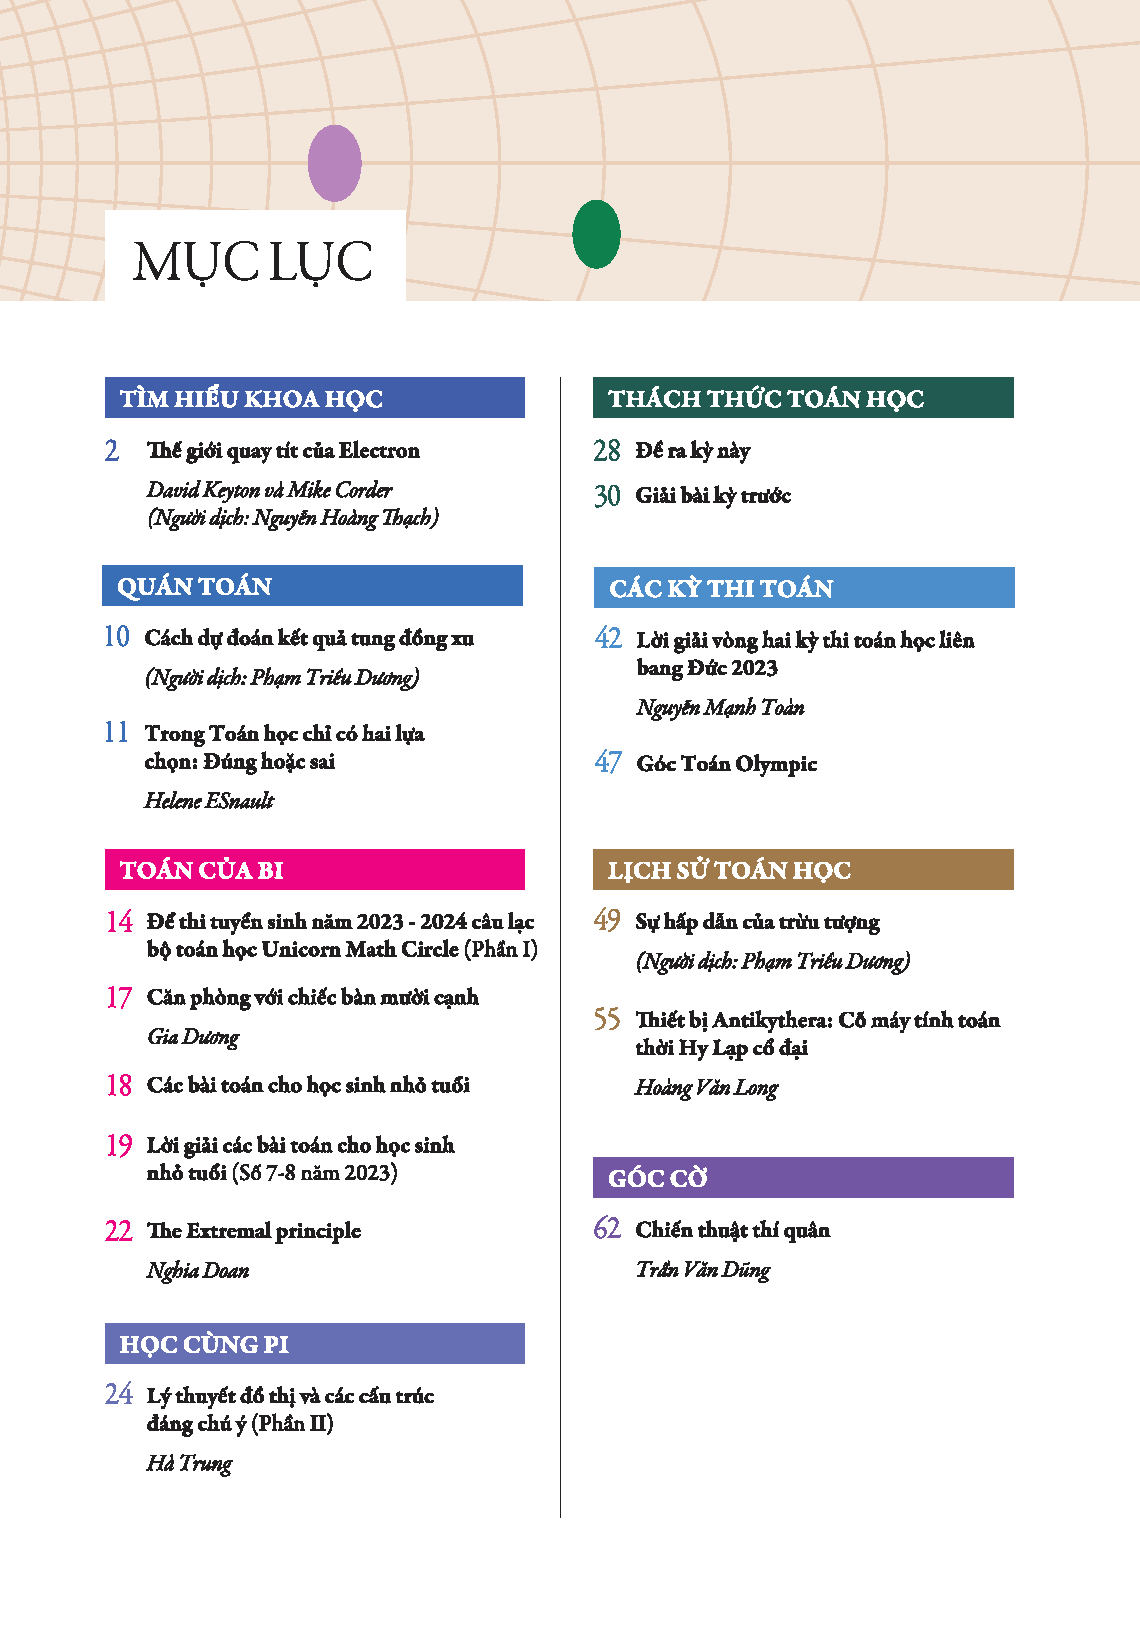
\includegraphics[scale=1]{ML.pdf}}}
%	 \centering
%	 \vspace*{0cm}
%	 \endgroup
%	 \newpage	  
%	 \pagestyle{empty}
%
%	\setcounter{page}{2}
%
%	\setcounter{figure}{0}
%	\thispagestyle{duongvaotoanhocnone}
\pagestyle{duongvaotoanhoc}
\everymath{\color{duongvaotoanhoc}}
\graphicspath{{../duongvaotoanhoc/pic/}}
\blfootnote{$^*$\color{duongvaotoanhoc}Xuất bản lần đầu trong: The Mathematical Intelligencer $10$, Springer, Berlin Heidelberg New York ($1975$) và được trích lại trong [$1$]}
\begingroup
\AddToShipoutPicture*{\put(0,616){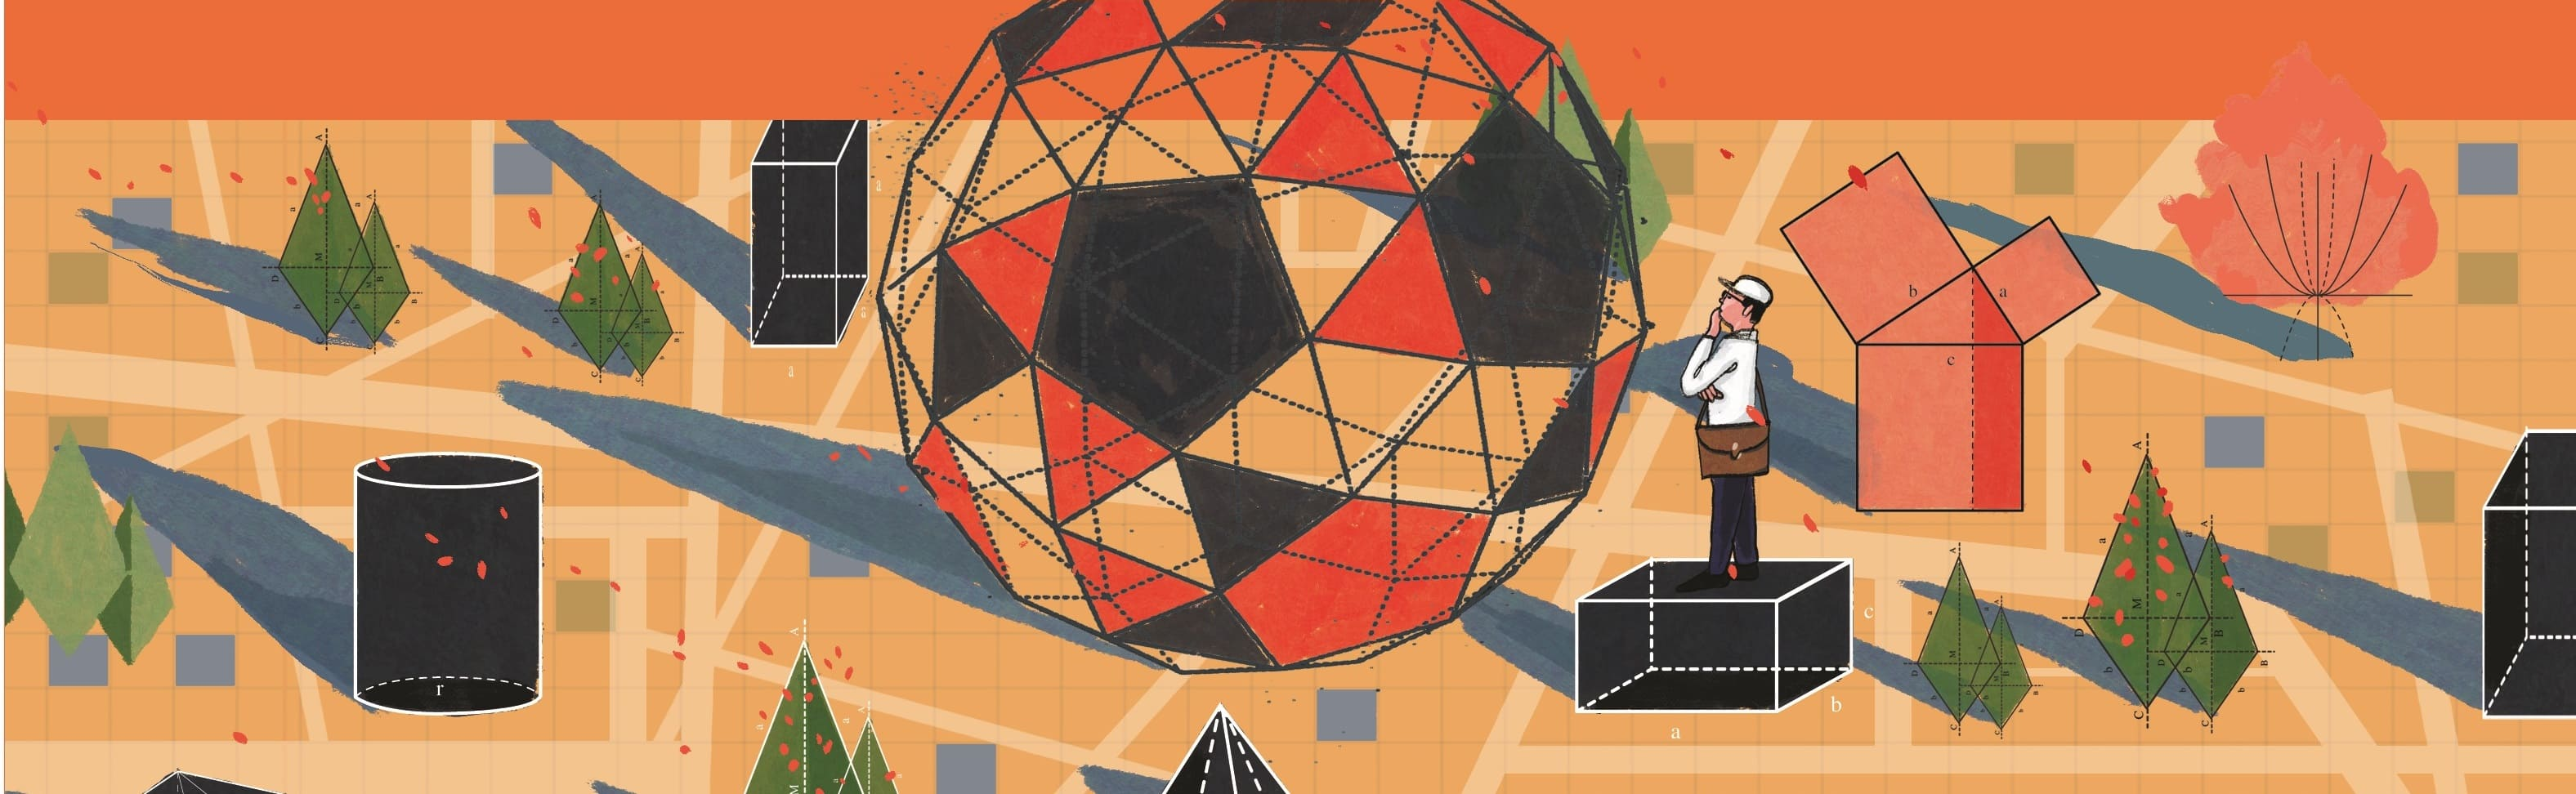
\includegraphics[width=19.3cm]{../bannerduongvao}}}
\AddToShipoutPicture*{\put(80,528){
\includegraphics[scale=1]{../tieude.pdf}}}
\centering
\endgroup

\vspace*{180pt}

\begin{multicols}{2}	
	Câu chuyện của ``các giả thuyết Weil" là một ví dụ kỳ diệu của trí tưởng tượng toán học, và là một trong những thí dụ đáng ngạc nhiên nhất biểu lộ sự thống nhất cơ bản của toán học. Những ý tưởng cốt lõi dẫn tới chứng minh của chúng tới từ sáu người: E. Artin, F. K. Schmidt, H. Hasse, A. Weil, A. Grothendieck, và P. Deligne, trong khoảng năm mươi năm ($1923-1973$).
	\vskip 0.1cm
	$\pmb{1.}$ \textbf{\color{duongvaotoanhoc}Số nghiệm của phương trình đồng dư}
	\vskip 0.1cm
	Một cách đủ thích hợp, câu chuyện, như mọi vấn đề trong lý thuyết số, bắt đầu từ Gauss. Trong công trình về luật thuận nghịch bình phương của mình, ông đưa ra cái ngày nay được gọi là tổng Gauss (phổ biến nhất là tổng $\sum_{x=0}^{p-1} \mathrm{exp}(2\pi i x^2/p)$ với $p$ nguyên tố); để tính các tổng này, bằng một số lập luận sơ cấp, ông suy ra cần tính số nghiệm của các phương trình đồng dư có các dạng 
	\begin{align*}
			&ax^3 - by^3 \equiv 1 \ (\mathrm{mod} \ p),\\ 
			& ax^4 - by^4 \equiv 1 \ (\mathrm{mod} \ p), \tag{$1$}\\ 
			&y^2 \equiv ax^4 - 1 \ (\mathrm{mod} \ p)  
	\end{align*}
	trong đó $a,b$ là các số nguyên cố định không chia hết cho $p$, nghiệm $(x,y)$ được xét theo đồng dư modulo $p$ (như vậy các phương trình đồng dư $(1)$ được xem như các phương trình trong trường $\mathbb{F}_p$); và $p$ \textit{chạy} trong một tập vô hạn các số nguyên tố; chúng ta đi tìm những biểu diễn \textit{tiệm cận} (dưới dạng những hàm đơn giản của $p$) của số lượng các nghiệm. Một thời gian ngắn sau, Jacobi nhận xét rằng, ngược lại, bằng cách sử dụng các tính chất cơ bản của tổng Gauss, ta có thể thu được một đánh giá tốt về số nghiệm trong các trường hợp tổng quát hơn, ở đó các phương pháp sơ cấp trở nên cồng kềnh. Sau Jacobi, gần như không có nhiều tiến triển trong chủ đề này cho tới khi Hardy và Littlewood, trong khi nghiên cứu bài toán Waring để đưa ra các tính chất của ``chuỗi kỳ dị", thấy rằng cần phải đưa ra một đánh giá tiệm cận cho số nghiệm của phương trình đồng dư
	\begin{align*}
		x_1^k + ... + x_r^k \equiv 0 \ (\mathrm{mod} \ p), \tag{$2$}
	\end{align*}
	trong đó $p$ là một số nguyên tố chạy tới $+\infty$. Hai ông đã sử dụng phương pháp của Jacobi cho mục đích này; tổng quát hơn, năm $1949$, cả Hua-Vandier và A. Weil đã độc lập chứng minh rằng phương pháp này có thể đánh giá số nghiệm $N$ của những phương trình
	\begin{align*} 
		a_0x_0^{k_0} \!+\! ... \!+\! a_r x_r^{k_r} \!=\! 0 \ (a_0,...,a_r \neq 0)\tag{$3$}
	\end{align*}
	trong mọi \textit{trường hữu hạn} $\mathbb{F}_{q}$ với $q = p^m$ phần tử; kết quả được đưa ra
	\begin{align*}
		N = q^r + O(q^{(r+1)/2}). \tag{$4$}
	\end{align*}
	Kết quả tương tự được đưa ra bởi Davenport $(1931)$ và Mordell $(1933)$ cho các phương trình dạng $y^m = P_n(x)$ trên $\mathbb{F}_p$, trong đó $P_n$ là một đa thức bậc $n$; với một số giá trị $m,n$ nhỏ, họ thu được các đánh giá có dạng $N  = p + O(p^{\phi(m,n)})$ trong đó $1/2 < \phi(m,n) < 1$.
	\vskip 0.1cm
	$\pmb{2.}$ \textbf{\color{duongvaotoanhoc}Về hàm Zêta}
	\vskip 0.1cm
	Hãy để chúng tôi nhắc lại các tính chất cổ điển của hàm zêta Riemann: nó xác định với $\mathscr{R}(s) > 1$ bởi chuỗi $\zeta(s) = \sum_{n=1}^{\infty} n^{-s}$, và thỏa mãn phương trình Euler
	\begin{align*}
		\zeta(s) = \prod_p (1 - p^{-s})^{-1} \tag{$5$}
	\end{align*}
	trong đó tích chạy trên tập tất cả các số nguyên tố. Riemann chứng minh rằng $\zeta$ có thể thác triển thành một hàm phân hình trên mặt phẳng phức với một cực duy nhất tại $s=1$, và nếu đặt
	\begin{align*} 
		\xi = \frac{1}{2}s(s-1)\pi^{-s/2}\Gamma(s/2)\zeta(s),
	\end{align*}
	thì $\xi$ là một hàm chỉnh hình trên toàn bộ mặt phẳng phức và thỏa mãn phương trình hàm $\xi(s) = \xi(1-s)$. Hơn nữa ông đề xuất \textit{giả thuyết Riemann} (vẫn chưa được chứng minh) rằng mọi nghiệm của $\xi$ nằm trên đường thẳng $\mathscr{R}(s)=1/2$. 
	\vskip 0.1cm
	Một thời gian ngắn sau, Dedekind mở rộng lý thuyết của Riemann lên một trường số $K$ (mở rộng hữu hạn của $\mathbb{Q}$), bằng cách định nghĩa $\zeta_K(s) = \sum_{\mathfrak{a}}(N\mathfrak{a})^{-s}$, trong đó $\mathfrak{a}$ chạy trên tất cả các ideal của vành $\mathfrak{o}$ các số đại số nguyên trong $K$, \textit{chuẩn} $N\mathfrak{a}$ là số phần tử của vành $\mathfrak{o}/\mathfrak{a}$. Ông mở rộng công thức Euler thành
	\begin{align*}
		\zeta_K(s) = \prod_{\mathfrak{p}} (1-  (N\mathfrak{p})^{-s})^{-1}, \tag{$6$}
	\end{align*}
	trong đó tích chạy trên tất cả các ideal nguyên tố $\mathfrak{p}$ của $\mathfrak{o}$; rất nhiều năm sau Hecke chứng minh rằng $\zeta_K$ có thể thác triển thành một hàm phân hình và thỏa mãn một phương trình hàm tương tự như phương trình hàm Riemann cho $\xi$. 
	\vskip 0.1cm
	Một cách hình thức, ta thấy rằng phương trình ($6$) chỉ dùng hai tính chất của vành $\mathfrak{o}$: $1)$ $\mathfrak{o}$ là một vành Dedekind: $2)$ trường $\mathfrak{o}/\mathfrak{p}$ là hữu hạn với mọi ideal nguyên tố $\mathfrak{p}$: thật vậy, nếu $\mathfrak{a} = \mathfrak{p}_1^{v_1}...\mathfrak{p}_r^{v_r}$ là một phân tích thành các ideal nguyên tố của ideal $\mathfrak{a}$ thì $\mathfrak{o}/\mathfrak{a}$ đẳng cấu với tích trực tiếp của các $\mathfrak{o}/\mathfrak{p}_i^{v_i}$, và với mọi ideal nguyên tố $\mathfrak{p}$, mỗi $(\mathfrak{o}/\mathfrak{p})$--module $\mathfrak{p}^h/\mathfrak{p}^{h+1}$ đẳng cấu với $\mathfrak{o}/\mathfrak{p}$; điều đó chứng tỏ rằng chuẩn là nhân tính, từ đó suy ra ($6$) một cách hình thức (chứng minh tính hội tụ của tích vô hạn cần một số ước lượng đơn giản về số các ideal nguyên tố với chuẩn cho trước). Năm $1923$, E. Artin nhận xét rằng các tính chất này đúng cho các vành định nghĩa theo cách sau: bắt đầu với một trường hữu hạn $\mathbb{F}_q$, xét trường $K_0 = \mathbb{F}_q(T)$ các phân thức hữu tỷ, và một mở rộng toàn phương $K = K_0(v)$ với $v^2=P(T)$, trong đó $P$ là một đa thức không có nghiệm bội. Khi đó bao đóng nguyên $\mathfrak{o}$ của $\mathbb{F}_q[T]$ trong $K$ thỏa mãn các tính chất $1)$ và $2)$, $\mathfrak{o}/\mathfrak{p}$ là một \textit{mở rộng hữu hạn} của $\mathbb{F}_q$ với mỗi ideal nguyên tố $\mathfrak{p}$; rất dễ để chứng minh chuỗi và tích vô hạn trong định nghĩa của $\zeta_K$ hội tụ với $\mathscr{R}(s)>1$. Hơn nữa Artin còn thấy rằng lý thuyết này đơn giản hơn của Dedekind rất nhiều, lý do là các hàm của ông có thể viết dưới dạng $Z(q^{-s})$ trong đó $Z(u)$ là một \textit{hàm hữu tỷ} với hệ số trong $\mathbb{Q}$; phương trình hàm biểu diễn thương $Z(1/qu)/Z(u)$ bởi một hàm hữu tỷ với không điểm và cực cho trước; ông ấy sau đó giả thuyết rằng không điểm của $Z(u)$ tất cả đều nằm trên đường tròn $\left| u \right| = q^{1/2}$ và tự kiểm chứng giả thuyết này với rất nhiều đa thức $P$ bậc nhỏ. 
	\vskip 0.1cm
	Bây giờ các ideal nguyên tố $\mathfrak{p}$ sao cho $\mathfrak{o}/\mathfrak{p} \cong \mathbb{F}_q$ ($N\mathfrak{p}=q$) tương ứng một-một với các đồng cấu $\mathfrak{o} \to \mathbb{F}_q$; mọi đồng cấu như vậy gửi $(T,v)$ tới $(a,b) \in \mathbb{F}_q^2$ thỏa mãn $b^2=P(a)$. Nói cách khác số nghiệm của phương trình $y^2 = P(x)$ trong $\mathbb{F}_q^2$ chính là số lượng $N_1$ các ideal nguyên tố kiểu này; tuy nhiên từ phương trình Euler ($6$) suy ra luôn rằng 
	\begin{align*} 
		\log Z(u) = N_1 u + \cdots 
	\end{align*}
	gần $u=0$, như vậy nghiên cứu $Z(u)$ giúp ta hiểu về $N_1$. ``Giả thuyết Riemann" của Artin sinh ra đánh giá
	\begin{align*}  
		\left|N_1 -q \right| \leq  c \cdot q^{1/2}, \tag{$7$}
	\end{align*}
	và như vậy làm chặt hơn những kết quả trước đó của ông về bài toán đồng dư của Gauss. 
	\vskip 0.1cm
	$\pmb{3.}$ \textbf{\color{duongvaotoanhoc}Bước vào hình học đại số}
	\vskip 0.1cm
	Cho $k$ là một trường giao hoán bất kỳ, người ta cố gắng hình dung tập nghiệm $(x_1,...,x_r) \in k^r$ của một phương trình $P(x_1,...,x_r)=0$, với $P$ là một đa thức bất khả quy trong $k[T_1,...,T_r]$ xem như một ``siêu mặt đại số affine" (``đường cong" với $r=2$, ``mặt" với $r=3$) trong ``không gian affine" $k^r$, Hơn nữa, với mọi mở rộng trường $K \supset k$, ta có thể xét các nghiệm của $P(y_1,...,y_r)$ với giá trị $y_i$ trong trường $K$ \textit{lớn hơn}, như vậy ta có một ``siêu mặt đại số" $V$ trong ``không gian affine" $K^r$; việc các hệ số của $P$ nằm trong $k$ giờ được thay bởi việc nói $V$ \textit{xác định} trên $k$. Kinh nghiệm cho thấy việc chuyển đổi giữa ngôn ngữ hình học và trực giác sang những đa tạp ``trừu tượng"chỉ có ích khi $K$ là \textit{đóng đại số} (hãy thử nghĩ về $x_1^2+x_2^2+1=0$ khi $k=\mathbb{R}$). Ta sẽ hạn chế sự quan tâm xuống trường hợp $K=\overline{k}$, bao đóng đại số của $k$; hơn nữa, ta chỉ xét các siêu mặt $V$ không kỳ dị trong $\overline{k}^r$, i.e. tại các điểm mà ``siêu phẳng tiếp xúc" được định nghĩa duy nhất theo nghĩa thông thường (có nghĩa là tất cả các đạo hàm riêng không đồng thời triệt tiêu trong $V$). Với mọi điểm $x=(x_1,...,x_r) \in V$, toạ độ $x_i$ nằm trong $\overline{k}$, do đó có một mở rộng hữu hạn nhỏ nhất $k(x)$ của $k$ chứa tất cả $x_j$ và $[k(x):k]=\mathrm{deg}(x)$ được gọi là \textit{bậc} của điểm $x$. Nếu $\mathfrak{m}$ là hạt nhân của đồng cấu $k[T_1,...,T_r] \to \overline{k}$ gửi mỗi $T_i$ tới $x_i$ thì $\mathfrak{m}$ là một ideal cực đại của $k[T_1,....,T_r]$ và $k[T_1,...,T_r]/\mathfrak{m}$ đẳng cấu với $k(x)$; ta viết $k(\mathfrak{m})=k(x)$ và $\mathrm{deg}(\mathfrak{m}) =\mathrm{deg}(x)$; có thể chứng minh rằng mọi ideal cực đại $\mathfrak{m}$ của $k[T_1,...,T_r]$ chứa $P(T_1,...,T_r)$ ứng với một điểm $x$ của $V$ với bậc $\mathrm{deg}(\mathfrak{m})$. 
	\vskip 0.1cm
	Khi $k=\mathbb{F}_q$, đặt
	\begin{align*}
		Z_V(u) = \prod_{P \in \mathfrak{m}}(1 - u^{\mathrm{deg}(\mathfrak{m})})^{-1}; \tag{$8$}
	\end{align*}
	hàm $Z(u)$ định nghĩa bởi E. Artin bằng với hàm $Z_C(u)$, trong đó $C$ là ``đường cong affine" $x_2^2 - P(x_1) = 0$ xác định trên $\mathbb{F}_q$. Một cách tổng quát ta gọi $Z_V$ là \textit{hàm zêta} của $V$. Các điểm của $V$ trong $(\mathbb{F}_q)^r$ là các điểm mà $\mathrm{deg}(x)$ là ước của $n$; hiển nhiên số lượng các điểm như vậy $\leq q^{nr}$, như vậy số lượng các ideal cực đại $\mathfrak{m}$ mà $P \in \mathfrak{m}$, tương ứng với các điểm này, có ước lượng \textit{tiên nghiệm} $\leq q^{nr}$, điều này chứng tỏ rằng ($8$) hội tụ với $u$ nhỏ; hơn nữa, với $u$ nhỏ ta có thể viết
	\begin{align*}
			uZ'_V(u)/Z_V(u) & = \sum_{P \in \mathfrak{m}} \frac{\mathrm{deg}(\mathfrak{m}) u^{\mathrm{deg}(\mathfrak{m})}}{1 - u^{\mathrm{deg}(\mathfrak{m})}} \\ 
			& = \sum_{v=1}^{\infty} \sum_{P \in \mathfrak{m}} \mathrm{deg}(\mathfrak{m}) u^{v\mathrm{deg}(\mathfrak{m})} \\
			&= \sum_{v=1}^{\infty} N_v u^v\tag{$9$}
	\end{align*}
	trong đó $N_v$ là số điểm của $V$ trong $(\mathbb{F}_{q^v})^r$.  
	\vskip 0.1cm
	Cách định nghĩa này có thể mở rộng cho các dạng đa tạp không kỳ dị khác, không nhất thiết phải bị nhúng trong ``không gian affine" $\overline{k}^r$. Nói một cách theo lịch sử, ngôn ngữ của hình học đại số trong lý thuyết của các hàm zêta được giới thiệu vào năm $1931$ bởi F. K. Schmidt, người nghiên cứu các \textit{đường cong xạ ảnh} không kỳ dị trên trường hữu hạn $\mathbb{F}_q$. Ông chứng minh rằng lý thuyết Dedekind--Weber của đường cong đại số trên $\mathbb{C}$ (bao gồm định nghĩa về giống và định lý Riemann--Roch) có thể mở rộng cho đường cong xạ ảnh trên một trường đóng đại số $\overline{k}$ bất kỳ; điều này cho phép ông chứng minh rằng với mọi đường cong xạ ảnh không kỳ dị $C$ với giống $g$ định nghĩa trên $\mathbb{F}_q$, hàm zêta có thể biểu diễn dưới dạng
	\begin{align*} 
		Z_C(u) = P_{2g}(u)/(1-u)(1-qu) \tag{$10$}
	\end{align*}
	trong đó tử số là một đa thức bậc $2g$ với hệ số nguyên và ta có một phương trình hàm
	\begin{align*} 
		Z_C(1/qu) = (qu^2)^{1-g}Z_C(u). \tag{$11$}
	\end{align*}
	``Giả thuyết Riemann" cho $C$ do đó nói rằng các không điểm của $P_{2g}$ nằm trên đường tròn $\left|u \right|=q^{1/2}$; dễ thấy điều này tương đương với bất đẳng thức
	\begin{align*} 
		\left|N_v \!-\! q^v\!-\! 1\right| \!\leq\! 2g \!\cdot\! q^{1/2} \ \text{với mọi} \ v \geq 1. \tag{$12$}
	\end{align*}
	$\pmb{4.}$ \textbf{\color{duongvaotoanhoc}Mơ mộng về Tôpô đại số}
	\vskip 0.1cm
	Quay lại trường hợp siêu mặt $V$ trong $(\overline{\mathbb{F}}_q)^r$, nhận xét rằng các phần tử của $\overline{\mathbb{F}}_q$ thuộc $\mathbb{F}_{q^n}$ chính là những phần tử mà $t^{q^n}=t$. Xét ánh xạ
	\begin{align*}
		\Phi: (x_1,...,x_r) \mapsto (x_1^{q},...,x_r^q)
	\end{align*}
	từ $(\overline{\mathbb{F}}_q)^r$ vào chính nó. Do hệ số của $P$ nằm trong $\mathbb{F}_q$, do đó thỏa mãn $t^q = t$, ta có
	\begin{align*}
		P(\Phi(x)) = (P(x))^q,
	\end{align*}
	do đó $\Phi$ ánh xạ $V$ lên chính nó; hạn chế của $\Phi$ lên $V$ được gọi là cấu xạ Frobenius của $V$. Năm $1936$, Hasse nhận thấy rằng với một đường cong $C$, số $N_v$ chính là số điểm $x \in C$ thỏa mãn $\Phi^v(x) = x$; i.e. $x$ là một \textit{điểm bất động} của $\Phi^v$. Bây giờ, chúng ta hãy bỏ qua chuỗi các sự kiện mang tính niên đại mà giả vờ rằng ta đang làm việc với các đa tạp đại số không kỳ dị ``cổ điển" $X$ trong một không gian xạ ảnh phức. Từ thời của Picard và  Poincaré người ta đã nhận thấy rằng hầu hết các tính chất của các đa tạp đại số được liên hệ chặt chẽ với các tính chất \textit{đồng điều}. Trong phiên bản hiện thời (chủ yếu từ các công trình của Lefschetz và Hodge), với một đa tạp xạ ảnh không kỳ dị bất khả quy $X$ chiều $d$ trên $\mathbb{C}$ (do đó là một đa tạp khả vi chiều $2d$), các tính chất này xoay quanh \textit{đại số đối đồng điều} $H^{\bullet}(X) = \bigoplus_i H^i(X)$ của $X$ trên trường $K$ với \textit{đặc số} $0$; nó là một đại số phân bậc trên $K$, thỏa mãn các tính chất sau:
	\vskip 0.1cm
	($A$) $1.$ Mỗi $H^i(X)$ là một $K$--không gian vector hữu hạn chiều, bằng $0$ ngoại trừ $0 \leq i \leq 2d$;
	\vskip 0.1cm
	$2.$ Tồn tại một đẳng cấu tự nhiên $H^{2d}(X) \overset{\sim}{\longrightarrow} K$, và với mỗi $i$, phép nhân trên $H^{\bullet}(X)$ cho ta một phép ghép cặp không kỳ dị $H^{i}(X) \times H^{2d-i}(X) \to H^{2d}(X) \overset{\sim}{\longrightarrow} K$ (đối ngẫu Poincaré) cho phép ta đồng nhất $H^{2d-i}(X)$ với 
	\begin{align*} 
		H_i(X) = \mathrm{Hom}_K(H^i(X),K),
	\end{align*} 
	\textit{đồng điều} của $K$ tại chiều $i$.
	\vskip 0.1cm
	$3.$ Với các đa tạp không kỳ dị $X, Y$, tồn tại một đẳng cấu tự nhiên của các đại số phân bậc 
	\begin{align*} 
		&H^{\bullet}(X) \otimes H^{\bullet}(Y) \cong H^{\bullet}(X \times Y) \\
		&\text{(công thức Kunneth)}.
	\end{align*}
	($B$) Mọi cấu xạ $f: X \to X$ định nghĩa tự nhiên, với mỗi $i$, một đồng cấu tuyến tính $f^{(i)}:H^i(X) \to H^i(X)$, sao cho các $f^{(i)}$ với $0 \leq i \leq 2d$ cảm sinh một đồng cấu $f^{\bullet}:H^{\bullet}(X) \to H^{\bullet}(X)$ của các đại số phân bậc. Các \textit{điểm bất động} của $f$ là phép chiếu lên $X$ của giao của đồ thị $\Gamma$ của $f$ và đường chéo $\Delta$ của $X \times X$; nếu $\Gamma$ giao \textit{hoành} với $\Delta$ tại mỗi điểm (nghĩa là các không gian tiếp xúc của chúng có giao chỉ là một điểm), số lượng điểm bất động của $f$ được tính bởi \textit{công thức vết Lefschetz}
		\begin{align*} \label{eq:13}
			N  = \sum_{i=0}^{2d} (-1)^i \mathrm{Tr}(f^{(i)}). \tag{$13$}
		\end{align*}
	($C$) Nếu $Y$ là một đa tạp con không kỳ dị của $X$ với chiều $d-1$, các ánh xạ tuyến tính tự nhiên $H^i(X) \to H^i(Y)$ là song ánh với $i \leq d-2$ và đơn ánh với $i = d-1$. 
	\vskip 0.1cm
	($D$) Lấy $h \in H^2(X)$ từ đối ngẫu Poincaré ứng với lớp đồng điều trong $H_{2d-2}(X)$ của một lát cắt siêu phẳng của $X$, và xét $L: a \to ha$ là phép nhân trái bởi $h$ trong $H^{\bullet}(X)$; khi đó $L^{d-i}: H^i(X) \to H^{2d-i}(X)$ là một đẳng cấu với $i \leq d$.
	\vskip 0.1cm
	Một lập luận đại số đơn giản cho thấy nếu một cấu xạ $f: X \to X$ thỏa mãn $f^{(2)}(h) = q \cdot h$ với $q > 0$ là một số hữu tỷ, và nếu $g_i = q^{-i/2}f^{(i)}$ (xem như một tự đồng cấu của $H^{i}(X) \otimes_K \overline{K}$), $g_i$ là song ánh, và $g_i^{-1}$ được đồng nhất với $\text{}^tg_{2d-i}$ bởi đối ngẫu Poincaré. Điều này suy ra rằng nếu $\alpha_{ij}$ là các giá trị riêng của $f^{(i)}$ trong $\overline{K}$, tập các phần tử $q^{i/2}\alpha_{ij}$ trùng với tập các phần tử $\alpha_{2d-i,j}/q^{d-(i/2)}$.
	\vskip 0.1cm
	($E$) Trong mỗi $H^i(X)$ với $i \leq d$ có một không gian con $A^i(X)$ ổn định dưới tác động của $f^{(i)}$ với mọi cấu xạ $f: X \to X$, và trên mỗi $A^i(X)$, ta có thể trang bị một cấu trúc không gian vector trên trường các số hữu tỷ cùng một \textit{tích vô hướng} không kỳ dị, sao cho: với mỗi $f$ thỏa mãn ($D$) thì mỗi $g_i$ là ánh xạ \textit{unita} với tích vô hướng này; điều này suy ra tất cả các giá trị riêng của $f^{(i)}$ (là các phần tử của $\overline{\mathbb{Q}}$) có giá trị tuyệt đối là $q^{1/2}$.
	\vskip 0.1cm
	Quay lại với siêu mặt $V$ xác định trên $\mathbb{F}_q$, \textit{giả sử} ta có thể gán với nó một đại số phân bậc $H^{\bullet}(V)$ có tất cả các tính chất vừa nêu, hơn nữa $\Phi^{(2)}(h) = q \cdot h$ trong đó $\Phi$ là đồng cấu Frobenius. Dễ thấy đồ thị của $\Phi^v$ giao hoành với $\Delta$; do đó, nếu $\alpha_{ij}$ là các giá trị riêng của $(\Phi^v)^{(i)}$, số $N_v$ có thể cho bởi công thức
	\begin{align*} 
		N_v = \sum_i (-1)^i \sum_j \alpha_{ij}^v;\tag{$14$}
	\end{align*}
	và do đó ta có (với $d= r-1=\mathrm{dim}(V)$)
	\begin{align*} \label{eq:15}
		Z_V(u) = \frac{P_1(u)P_3(u)...P_{2d-1}(u)}{P_0(u)P_2(u)...P_{2d}(u)} \tag{$15$}
	\end{align*}
	trong đó $P_i(u) = \mathrm{deg}(1 - u \cdot \Phi^{(i)})$ là một đa thức với hệ số nguyên. Nói riêng, $Z_V(u)$ là một hàm \textit{hữu tỷ}; hơn nữa $Z_V(1/q^d u)$ nên có không điểm và cực giống với $Z_V(u)$ ngoại trừ khi $u=0$, và ta nên có $\left|\alpha_{ij}\right|=q^{1/2}$. Cuối cùng, nếu tất cả hệ số của $V$ là các lớp đồng dư mod $p$ của các số nguyên, hệ số của một phương trình của một đa tạp không kỳ dị $V_0$ trong $\overline{\mathbb{Q}}^r$, bậc của mỗi $P_i$ sẽ bằng số Betti thứ $i$ của $V_0$. 
	\vskip 0.1cm
	Các phát biểu trên là \textit{các giả thuyết Weil} cho $Z_V$.
	\vskip 0.1cm
	$\pmb{5.}$ \textbf{\color{duongvaotoanhoc}Những ``phương án thay thế" cho đối đồng điều của Hasse và Weil} 
	\vskip 0.1cm
	Để hiểu tại sao Weil đã có thể đi tới những khái niệm táo bạo như vậy, ta phải quay lại những ý tưởng đầu tiên của Hasse trong việc chứng minh ``giả thuyết Riemann" cho các đường cong \textit{giống} $1$ trên $\mathbb{F}_q$. Trong lý thuyết cổ điển của các đường cong không kỳ dị trên trường số phức, mỗi đường cong $C$ được gán với \textit{jacobian} $J = J(C)$, có thể xem như đối ngẫu Pontrjagin của nhóm đồng điều $H_1(C,\mathbb{Z})$; đối ngẫu này được dẫn ra từ dạng song tuyến tính $(\gamma,\omega) \mapsto \int_{\gamma}\omega$ định nghĩa trên các chu trình $\gamma$ và các dạng vi phân abel chỉnh hình $\omega$ trên diện Riemann $C$ (``chu kỳ" của $\omega$ trên $\gamma$). Nếu $C$ có giống $g$ thì $J(C)$ là một xuyến phức $\mathbb{C}^g/\Delta$ trong đó $\Delta$ là một nhóm con rời rạc với hạng $2g$, thỏa mãn các điều kiện song tuyến tính Riemann cổ điển. Ta có thể định nghĩa $J$ một cách đại số, bằng cách xét các nhóm cộng $G/G_i$ của các lớp của các ước bậc $0$ trên $C$, modulo quan hệ tương đương tuyến tính: ta gắn mỗi ước $D$ bậc $0$, vốn có thể viết dưới dạng $\partial \gamma$ với $1$-xích $\gamma$ trên diện Riemann, một lớp $\phi(D)$ trong $\mathbb{C}^g/\Delta$ của vector $\left(\int_{\gamma}\omega_1,...\int_{\gamma}\omega_g\right)$, trong đó các $\omega_j$ lập thành một cơ sở của không gian các dạng vi phân chỉnh hình; định lý Abel-Jacobi nói rằng phép tương ứng này là toàn ánh và có hạt nhân $G_i$. Từ đó có thể trang bị cho $J$ một cấu trúc \textit{nhóm đại số} (một trường hợp cụ thể của nhóm đại số trên $\mathbb{C}$ được biết đến như \textit{các đa tạp abel}) với sự giúp đỡ của các điều kiện (siêu việt) song tuyến tính Riemann. Cuối cùng, nếu $x_0$ là một điểm trên $C$,
	\begin{align*}
		x \mapsto \phi((x) - (x_0))
	\end{align*}
	là một cấu xạ từ $C$ vào $J$ và là đẳng cấu nếu $g=1$.
	\vskip 0.1cm
	Phương pháp đầu tiên của Hasse để làm việc với các đường cong $C$ giống $1$ xác định trên $\mathbb{F}_q$ là ``nâng" $C$ thành một đường cong $C_0$ ``cổ điển" giống $1$ xác định trên trường các số hữu tỷ $\mathbb{Q}$: nếu $E$ là trường các hàm hữu tỷ trên $C$, ông chứng minh rằng ta có thể xác định $C_0$ sao cho, nếu $\omega_1,\omega_2$ là các hàm chu kỳ của các hàm elliptic ứng với $C_0$ (nên trường $E_0$ của các hàm này là trường các hàm hữu tỷ trên $C_0$), $\omega_1/\omega_2$ phải sinh ra một trường toàn phương ảo $K$ trên $\mathbb{Q}$, và $E$ sẽ là trường thặng dư của vành các số nguyên của $K$ modulo một ideal nguyên tố khéo chọn nào đó. Hasse từ đó đã có thể dùng các kết quả cổ điển về ``các phép nhân phức" của $C_0$ (i.e. tự đồng cấu của jacobian $J(C_0)$) để xác định số điểm của $C$ với bậc $1$, và chứng minh ``giả thuyết Riemann" cho $C$.
	\vskip 0.1cm
	Một thời gian ngắn sau, Hasse từ bỏ phương pháp trên và thay thế bằng một phương pháp có tính nội tại hơn: như đã nói ở trên, $J(C)$ có thể định nghĩa một cách đại số như một nhóm ``trừu tượng", và cấu xạ Frobenius định nghĩa tự nhiên một tự đồng cấu của nhóm đó; Hasse chứng minh rằng tử số của hàm zêta $Z_C$ trong ($10$) (trong trường hợp này là một đa thức bậc $2$) được đồng nhất với đa thức đặc trưng của tự đồng cấu đó. Công cụ mà ông giới thiệu cho mục đích này là một số nguyên $v(\lambda)$ gắn với mỗi tự toàn cấu $\lambda$ của $J(C)$: nếu $E$ là trường các hàm hữu tỷ của $C$, $\lambda$ định nghĩa một ``đối cấu xạ" (comorphism) $R(\lambda)$, một tự đẳng cấu của $E$ và $v(\lambda)$ là bậc $[E:R(\lambda)(E)]$, hữu hạn khi $\lambda$ là toàn cấu. Hasse chứng minh rằng với mọi số nguyên $a,b$ thì
	\begin{align*} v(a.1 + b.\lambda) = a^2 + \sigma(\lambda)ab + v(\lambda)b^2
	\end{align*} 
	với mọi tự toàn cấu $\lambda$ của $J(C)$, tính xác định dương của dạng toàn phương này cho ông chứng minh của ``giả thuyết Riemann". 
	\vskip 0.1cm
	Việc mở rộng những ý tưởng này cho các đường cong $C$ giống $g$ bất kỳ trên $\mathbb{F}_q$ là không hề hiển nhiên: lý thuyết cổ điển chứng minh rằng $J(C)$ nên là một nhóm đại số $g$ chiều (thay vì đẳng cấu với $C$ như một đa tạp đại số trong trường hợp của Hasse), và cho tới tận năm $1940$ không ai mở rộng lý thuyết của các nhóm đại số trên trường đặc số $p>0$ sang hình học đại số, và nói riêng lý thuyết của các đa tạp abel. Điều này đã được thực hiện một mình bởi A. Weil, người đầu tiên phải phát triển, trong cuốn sách nổi tiếng \textit{Foundations of algebraic geometry}, các tính chất cơ bản của các số giao một cách độc lập mà không viện tới tôpô đại số. Sau đó ông đã có thể nghiên cứu cấu trúc vành của các tự đồng cấu của một đa tạp abel $A$; với mọi tự toàn cấu $\lambda$ của $A$, Weil định nghĩa số nguyên $v(\lambda)$ như Hasse, (bây giờ $E$ là trường các hàm hữu tỷ trên $A$) và lần này chứng minh
	\begin{align*}
		&v(a \cdot 1 + b \cdot \lambda) \\
		= \,&a^{2g} + \sigma(\lambda)a^{2g-1}b +...+ v(\lambda)b^{2g}.
	\end{align*}
	Bất biến $\sigma(\lambda)$ được xem như một ``thay thế" đóng vai trò của $\mathrm{Tr}(f^{(1)})$ khi $\lambda$ là tự đồng cấu của $J(C)$ ứng với một cấu xạ $f$ của $C$. Một ``thay thế" cho đối ngẫu Poincaré được phát hiện trong một đối ngẫu tổng quát cho các đa tạp abel mà có thể định nghĩa nghĩa hoàn toàn đại số (trong trường hợp cổ điển người ta định nghĩa nó bởi đối ngẫu Pontrjagin); cuối cùng, nếu $\lambda'$ là ``chuyển vị" của một tự đồng cấu $\lambda$ trong đối ngẫu này thì ta có thể chứng minh $\sigma(\lambda \lambda') > 0$ với $\lambda \neq 0$, tính chất này (xem như một ``thay thế" cho tính xác định dương của tích vô hướng Hodge) cho phép Weil đưa ra chứng minh của ``giả thuyết Riemann" cho đường cong có giống bất kỳ.
	\vskip 0.1cm
	Trong tất cả các công trình này, Weil đã không ngừng giữ trong trí óc ông lý thuyết cổ điển của các ``tương ứng" phát triển bởi Hurwicz: một tương ứng trên $C$ có thể xem như một cấu xạ ``đa trị", mà cụ thể hơn như một đường cong $\Gamma$ trên diện $C \times C$; tốt hơn nữa, nó được định nghĩa như một ước (tổ hợp tuyến tính của các đường cong) trên $C \times C$. Một tương ứng $\Gamma$ gắn một cách tự nhiên (bắt chước phiên bản lý thuyết tập hợp) mỗi ước $D$ trên $C$ (tổ hợp tuyến tính của các điểm) một ước khác $\Gamma(D)$, một lần nữa điều này định nghĩa một tự đồng cấu của $J(C)$; ngược lại có thể chỉ ra rằng mọi tự đồng cấu của $J(C)$ đều thu được từ cách định nghĩa này. Trong trường hợp cổ điển, công thức Lefschetz ($13$) có thể được mở rộng để cho số giao của một tương ứng $\Gamma$ với ``tương ứng đồng nhất", i.e. đường chéo $\Delta$ của $C \times C$, và thực tế điều này đã được chứng minh bởi Hurwicz vào năm $1866$, sử dụng lý thuyết tích phân abel; sự thật là Weil đã có thể chứng minh một công thức tương tự bằng các công cụ thuần túy đại số, điều đã dẫn ông đến chỗ đề xuất các giả thuyết mang tên mình.
	\vskip 0.1cm
	$\pmb{6.}$ \textbf{\color{duongvaotoanhoc}Đối đồng điều \'etale và định lý của Deligne}
	\vskip 0.1cm
	Sử dụng kết quả của mình cho các đường cong, Weil đã chứng minh được các giả thuyết của chính ông với các siêu mặt dạng ($3$), cũng như cho những đa tạp khác như các đa tạp Grassman. Nhưng tại thời điểm đó không có một lý thuyết đối đồng điều nào đủ ``tốt" đã được định nghĩa. Khoảng năm $1953$, Cartan và Serre đã dùng đối đồng điều Leray với hệ số là các bó như một công cụ cực kỳ hữu hiệu để nghiên cứu các đa tạp phức, và Serre đã chỉ ra làm cách nào để chuyển các kỹ thuật này sang các đa tạp đại số trên một trường đóng đại số với đặc số $p$. Nhưng khi $p>0$, những nhóm đối đồng điều mới đó được định nghĩa hiển nhiên không thể được sử dụng bởi công thức Lefschetz ($13$), trong đó vế trái bắt buộc phải là một số nguyên, mà không phải một phần tử của một trường có đặc số $p$. Chỉ sau khi Grothendieck xây dựng lý thuyết lược đồ mà, từ một lưu ý của Serre, thì cậu ấy đã có thể mở rộng ý tưởng ban đầu theo cả hai hướng ``tôpô" và ``bó", gắn mỗi đa tạp (hoặc lược đồ) $X$ một đại số đối đồng điều $H^{\bullet}(X_{et},\mathbb{Q}_l)$ trên trường $l$--adic $\mathbb{Q}_l$, trong đó $l$ là một số nguyên tố khác với đặc số của trường ban đầu (sự can thiệp của các trường $l$--adic trong những câu hỏi này đã được nhận ra bởi Weil và Deuring).
	\vskip 0.1cm
	Độ sâu sắc và phức tạp của các kỹ thuật liên quan trong định nghĩa của ``đối đồng điều \'etale" $H^{\bullet}(X_{et})$ như thể để loại trừ mọi khả năng trong việc đưa ra bất kỳ một chi tiết nào nữa trong định nghĩa của nó. Hãy để chúng tôi chỉ ra Grothendieck (với sự giúp đỡ của M. Artin (con trai của E. Artin) và J. L. Verdier) đã có thể chứng minh các tính chất ($A$), ($B$), ($C$) \footnote[1]{\color{duongvaotoanhoc}Trước khi đối đồng điều $l$--adic được định nghĩa, Dwork đã chứng minh, bằng cách khéo léo sử dụng các hàm giải tích $p$--adic, rằng hàm zêta $Z_V(u)$ là \textit{hữu tỷ}.} ở trên và gần đây Deligne đã chứng minh ($D$) cũng đúng với mọi đa tạp trên một trường hữu hạn $\mathbb{F}_q$; tuy nhiên không một tính chất nào tương tự như ($E$) đã được chứng minh cho đối đồng điều \'etale (hoặc bất kỳ một lý thuyết đối đồng điều nào được đưa ra gần đây). Các tính chất ($A$), ($B$), ($C$) là đủ để chứng minh ($15$), cũng như phương trình hàm
	\begin{align*}
		Z_V(1/q^d u) = \pm q^{n\chi/2} u^{\chi}Z_V(u)
	\end{align*}
	trong đó
	\begin{align*}
		\chi = \sum_{i=0}^{2d} (-1)^i \mathrm{dim} \ H^i(X_{et},\mathbb{Q}_l).
	\end{align*}
	Tuy nhiên, chỉ đến gần đây người ta mới biết rằng các hệ số của $P_j$ trong ($15$) là độc lập với số nguyên tố $l$. Điều này cuối cùng cũng được chứng minh bởi Deligne năm $1973$, cùng với phần cuối và khó nhất của các giả thuyết Weil là $\left|\alpha_{ij}\right|=q^{1/2}$.
	\vskip 0.1cm
	Ở đây lần nữa, cần nhớ rằng không thể mô tả một cách chi tiết các chứng minh cực kỳ khéo léo, điều này hơi khác với chứng minh của Hasse và Weil, do nó không thể dựa trên một lập luận ``tính dương". Ta hạn chế bài toán xuống trường hợp $i=d$ (i.e. đối đồng điều ``trung tâm" $H^d(X)$); việc chứng minh rằng $\left|\alpha_{dj}\right|=q^{d/2}$ thì tương đương với
	\begin{align*} \label{eq:18}
		q^{(d-1)/2} \leq \left|\alpha_{dj}\right| \leq q^{(d+1)/2} \tag{$18$}
	\end{align*}
	bởi vì nếu ta áp dụng kết quả này với tích $X^k$, và sử dụng công thức Kunneth, ta có
	\begin{align*} 
		q^{(kd-1)/2} \leq \left|\alpha_{dj}^k \right| \leq q^{(kd+1)/2}
	\end{align*}
	sau đó cho $k$ tiến tới $+\infty$ và thu được kết quả. Thậm chí trong ($18$) ta có thể giả sử là $d$ chẵn và sau đó có thể chứng minh bằng quy nạp theo số chẵn $d$; đây là một bước sâu sắc và khó trong chứng minh, dựa trên kỹ thuật ``đơn đạo" cũ từ Picard và Lefschetz: kỹ thuật này hoàn toàn mang tính tôpô trong trường hợp cổ điển, nhưng nó cũng đã được chuyển sang đối đồng điều \'etale bởi Grothendieck và những người cùng trường phái của cậu ấy.
	\vskip 0.1cm
	Như thường thấy trong toán học, sự đột phá này mở ra một con đường trong việc khai phá các vấn đề mới; nhưng chừng nào bài toán ban đầu của Gauss còn được quan tâm, nó là điểm cuối của vấn đề, vì định lý của Deligne suy ra rằng, số các điểm bậc $1$ của một siêu mặt xạ ảnh không kỳ dị $d$ chiều thỏa mãn đánh giá
	\begin{align*} 
		\left| N - (1 + q+...+q^d )\right| \leq bq^{d/2}
	\end{align*}
	trong đó thậm chí hằng số $b$ có thể tính cụ thể: nó là số Betti thứ $d$ của các siêu mặt trên $\mathbb{C}$ có cùng bậc với $V$.
	\vskip 0.1cm
	\textbf{\color{duongvaotoanhoc}Tài liệu tham khảo}
	\vskip 0.1cm
	[$1$] Eberhard Freitag and Reinhardt Kiehl. \textit{Étale cohomology and the Weil conjecture}, volume $13$ of \textit{Ergebnisse der Mathematik und ihrer Grenzgebiete ($3$) [Results in Mathematics and Related
	Areas ($3$)]}. Springer--Verlag, Berlin, $1988$. Translated from the German by Betty S. Waterhouse and William C. Waterhouse, With an historical introduction by J. A. Dieudonné.
\end{multicols}
\vspace*{-10pt}
{\rule{1\linewidth}{0.1pt}}
\vskip 0.25cm
\centerline{\LARGE\textbf{\color{duongvaotoanhoc}LỜI GIẢI, ĐÁP ÁN}}
\begin{multicols}{2}
		\textbf{\color{duongvaotoanhoc}Đố vui}
		\vskip 0.1cm
		Hãy hình dung khối lập phương bao gồm tám khối lập phương đơn vị.
		\begin{figure}[H]
				\vspace*{-10pt}
				\centering
				\captionsetup{labelformat= empty, justification=centering}
				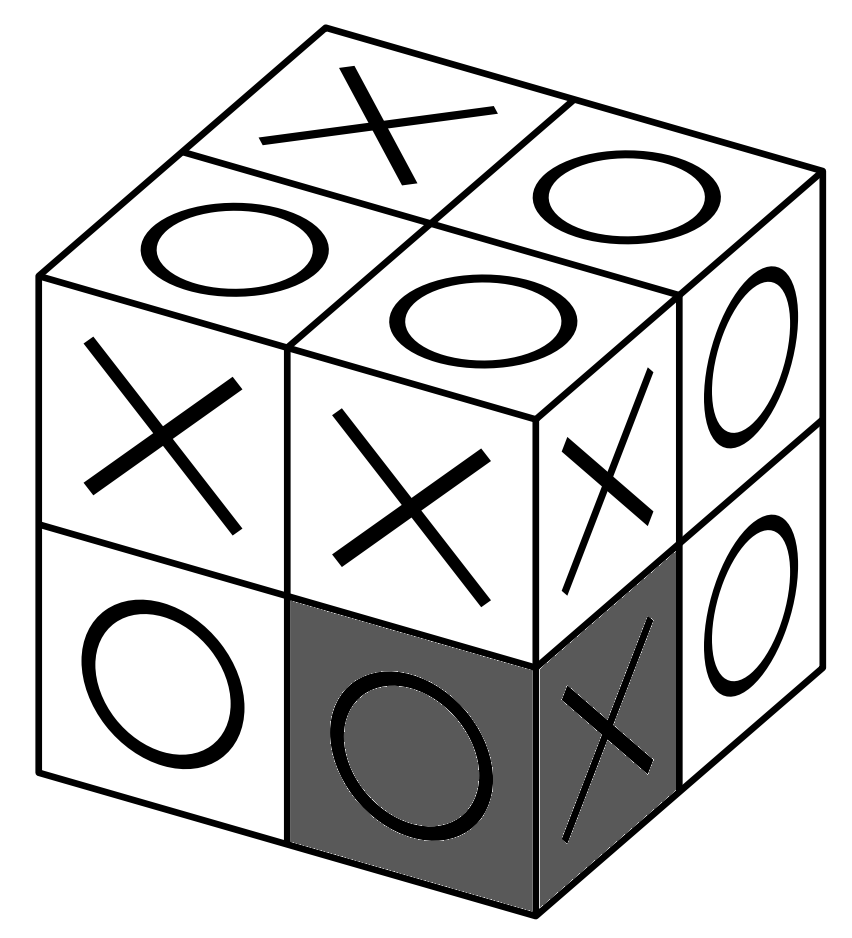
\includegraphics[width= 0.65\linewidth]{lgdovui}
		%		\caption{\small\textit{\color{}}}
				\vspace*{-5pt}
			\end{figure}
		Hãy quan sát khối lập phương đơn vị được tô màu xám như trong hình. Cho dù Bi có điền dấu gì ở mặt bên dưới của khối lập phương này thì cũng không thỏa mãn yêu cầu của thầy giáo: nếu bạn điền dấu $X$ thì mặt chứa dấu $O$ sẽ được bao quanh bởi $3$ ô có dấu $X$ và $1$ ô có dấu $O$, còn nếu bạn điền dấu $O$ thì mặt chứa dấu $X$ sẽ được bao quanh bởi $3$ ô có dấu $O$ và $1$ ô có dấu $X$!
\end{multicols}
%	\newpage
%
%	\setcounter{figure}{0}
%	\thispagestyle{quantoannone}
\pagestyle{quantoan}
\everymath{\color{quantoan}}
\graphicspath{{../quantoan/pic2/}}
\blfootnote{\color{quantoan}$^1$Viện Vật lý.}
\begingroup
\AddToShipoutPicture*{\put(0,616){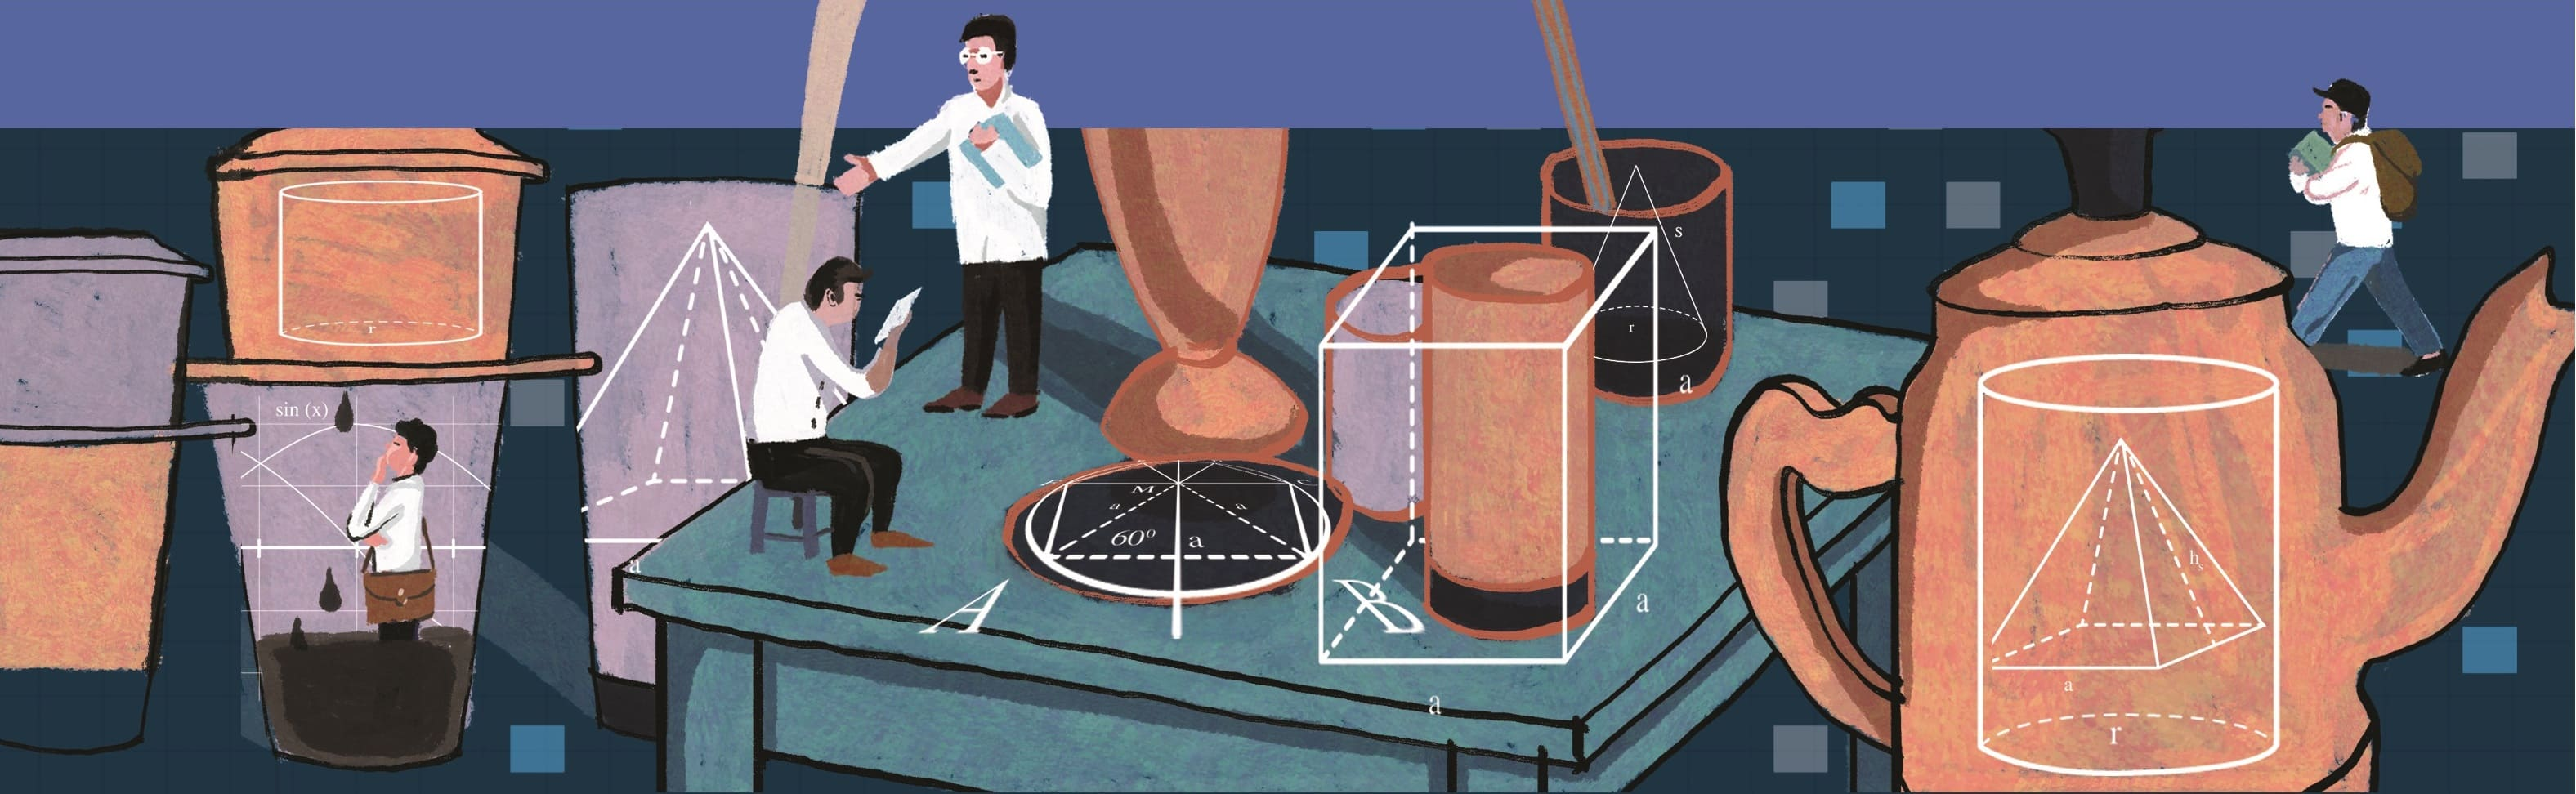
\includegraphics[width=19.3cm]{../bannerquantoan}}}
\AddToShipoutPicture*{\put(132,550){
\includegraphics[scale=1]{../tieude2.pdf}}}
\centering
\endgroup
\vspace*{160pt}

\begin{multicols}{2}
	Richard Feynman ($1918-1988$, Mỹ) nổi tiếng là người trung thực không khoan nhượng và đam mê đến tận cùng. Về tính trung thực, người ta hay nhắc đến vụ ông trình diễn trực tiếp trên TV một ``thí nghiệm nhỏ", bỏ vòng cao su vào cốc nước đá, minh chứng rằng cao su mất tính đàn hồi ở nhiệt độ thấp, qua đó chỉ ra nguyên nhân dẫn đến thảm họa tàu vũ trụ con thoi ``Challenger", vạch trần chiến dịch tung hỏa mù của NASA về nguyên nhân của thảm họa này. Để công bố với người dân Mỹ sự thật ấy, Feynman đã phải vượt qua sức ép khủng khiếp từ các cơ quan công quyền Mỹ, trong đó có CIA và NASA. 
	\vskip 0.1cm
	Feynman lắm đam mê. Đam mê vật lý, Feynman nhận giải Nobel Vật lý năm $1965$. Đam mê chơi trống, vở ba--lê do ông đệm trống nhận giải nhất trong cuộc thi ba--lê toàn nước Mỹ và giải nhì trong cuộc thi quốc tế tại Paris. Đam mê vẽ, ông đã có triển lãm tranh riêng. Không rõ ông biết những ngôn ngữ nào, chỉ biết thăm Brazil ông dạy bằng tiếng Bồ, thăm Nhật ông giao du bằng tiếng Nhật. Rồi có lần bạn bè định ``cho ông một vố", họ nhờ một cô Hoa kiều đón tiếp ông bằng tiếng Trung, Feynman đáp lại và cô ấy kêu trời, vì ông nói tiếng Quảng Đông, còn cô chỉ nói tiếng Bắc Kinh. Rất nhiều ``đam mê" kiểu như vậy được kể trong cuốn ``Feynman, chuyện thật như đùa" (NXB Trẻ) và hầu như tất cả đều có kết cục mỹ mãn, kiểu như giải Nobel. Có thể bạn nghĩ chắc ông này ``con nhà nòi", học ``trường quốc tế" từ nhỏ! Xin thưa, bố của Feynman là người bán rong bán quần áo, còn mẹ thì nội trợ. 
	\begin{figure}[H]
		\vspace*{-5pt}
		\centering
		\captionsetup{labelformat= empty, justification=centering}
		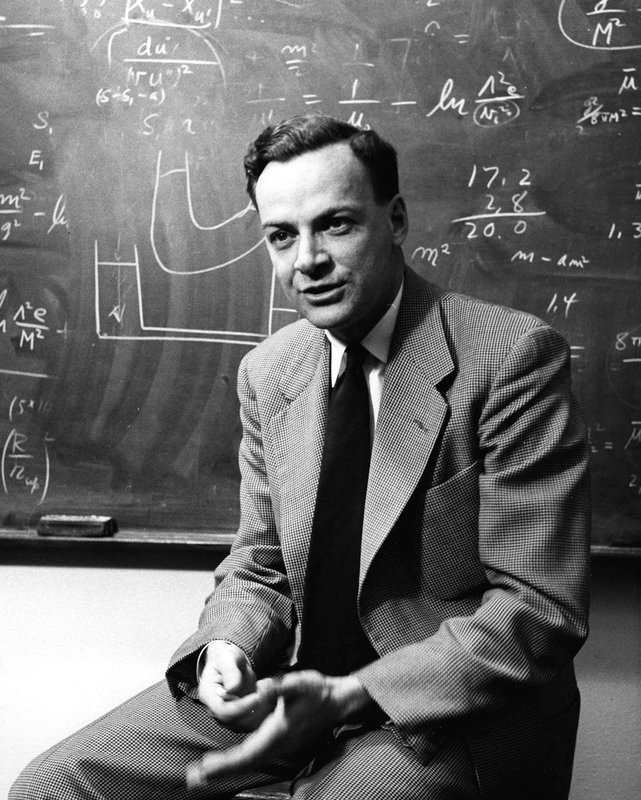
\includegraphics[width= 1\linewidth]{1a}
		\caption{\small\textit{\color{quantoan}Richard Feynman (ảnh từ bộ sưu tập của Viện Công nghệ California -- CalTech).}}
		\vspace*{-10pt}
	\end{figure}
	Ông chơi trống bongo cực giỏi, nhưng chưa bao giờ học nhạc lý. Ông vốn vẽ rất kém, tự nhận chẳng thể vẽ nổi cái gì ngoại trừ cái kim tự tháp chỉ gồm mấy đường thẳng. Để học vẽ, Feynman ``đổi công" với một họa sỹ: ông dạy vật lý cho họa sỹ còn họa sỹ dạy vẽ cho ông. Hãy tưởng tượng một giáo sư nổi tiếng thế giới ngồi trong lớp vẽ cùng các cháu $8-9$ tuổi học cách gọt bút chì. Đam mê như thế chỉ có ở Feynman. Và, với ông đam mê chính là nguồn cội của thành công, chứ chẳng phải ``con nhà nòi" hay ``trường quốc tế" nào cả. Tiền bạc và chứng chỉ đầy người, mà không đam mê gì, thì làm sao có thành quả! 
	\begin{figure}[H]
		\vspace*{-5pt}
		\centering
		\captionsetup{labelformat= empty, justification=centering}
		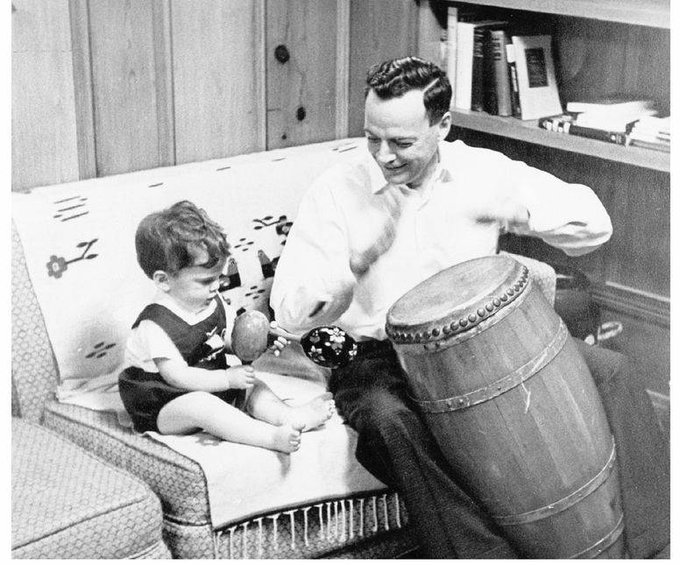
\includegraphics[width= 1\linewidth]{2a}
		\caption{\small\textit{\color{quantoan}Feynman chơi trống bên con trai (ảnh từ Internet).}}
		\vspace*{-10pt}
	\end{figure}
	Duy có đam mê cuối cùng, Feynman đã không kịp nhìn thấy những gì mình muốn, trước khi về cõi vĩnh hằng. Đó là ``Cuộc phiêu lưu cuối cùng của Feynman"\footnote[2]{\color{quantoan}Xem thêm: Cuộc phiêu lưu cuối cùng của Feynman, in lần $2$, NXB Trẻ, $2023$.}. Cuộc phiêu lưu khởi đầu bằng một con tem có xuất xứ từ một nơi gọi là Tannu Tuva, mà Feynman có được từ khi còn nhỏ. Cái tên ``Tuva" xa lạ nằm yên trong đầu Feynman, cho đến một ngày hè $1977$ nó trở thành mục tiêu cho ``cuộc phiêu lưu" kéo dài hơn $10$ năm cuối của cuộc đời ông. Tôi cược là nhiều bạn chưa biết Tuva là địa danh nào và ở đâu. Để đỡ tra cứu, xin ``bật mí" ngay: đó là tên một quốc gia nhỏ nằm giáp phía Tây Bắc của Mông Cổ, vốn độc lập, nhưng đã sáp nhập vào Liên Xô cũ (và Nga ngày nay). Thủ đô của Tuva là Kyzyl. Tuva có gì đặc biệt mà khiến Feynman mê mệt đến vậy?
	\vskip 0.1cm
	Bạn có biết đâu là trọng tâm của châu Á (lục địa thôi chứ không tính các đảo)? Lấy tấm bìa cứng phẳng, vẽ lên đó bản đồ châu Á, cắt theo đường biên để được miếng bìa hình châu Á lục địa. Dùng một chiếc bút đầu nhọn chống phía dưới tấm bìa, di di đầu bút, để tìm vị trí mà tấm bìa nằm cân bằng trên chiếc bút thẳng đứng. Vị trí đó rơi vào Kyzyl, trọng tâm của châu Á. Tất nhiên, các nhà khoa học xác định điểm này bằng các phương pháp chính xác hơn, và ngày nay ở Kyzyl có tấm bia lớn khẳng định vị trí đặc biệt của thành phố này. Nhưng, chỉ chừng ấy thì không đủ để Feynman mất tới cả chục năm tìm cách tới thăm Tuva.
	\begin{figure}[H]
		\vspace*{-5pt}
		\centering
		\captionsetup{labelformat= empty, justification=centering}
		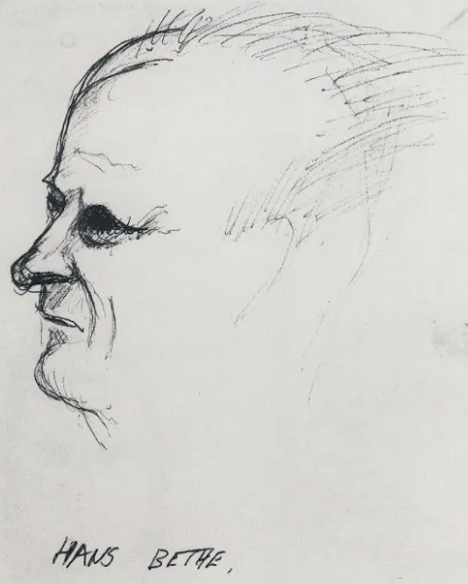
\includegraphics[width= 1\linewidth]{3a}
		\caption{\small\textit{\color{quantoan}Feyman vẽ Hans Bethe (giải Nobel Vật lý $1967$).}}
		\vspace*{-10pt}
	\end{figure}
	Cái chính là ở quốc gia tí xíu bao bọc bởi những dãy núi cao ấy, thời gian gần như ngừng trôi: tất cả vẫn nguyên sơ như $500$ hay $1000$ năm trước. Thảo nguyên hoang dại. Những đàn tuần lộc hay bò Tây Tạng cũng dường như hoang dại. Cuộc sống du mục không thể tự nhiên hơn. Một nền văn hóa xa xưa và kỳ thú với kiểu hát hai giọng chỉ có ở Tuva, với thứ văn tự không thể tìm thấy trong bất cứ tự điển nào, với các tập tục rất lạ điều hành bởi các tù trưởng uy nghi và bí ẩn v.v. Tiếc là ít người biết Tuva, chứ không, người ta đã gọi quốc gia này là ``Thảo nguyên Xanh" cuối cùng của hành tinh Trái Đất (như Congo là Hành tinh Xanh cuối cùng). Đam mê Tuva, Feynman tìm đọc mọi tài liệu về Tuva, tìm hiểu văn tự Tuva, học cách hát của dân du mục Tuva, ăn mặc và trang trí như tù trưởng Tuva \ldots Và, nhất là, ông tìm mọi cách để có thể đến thăm Tuva.
	\vskip 0.1cm
	Đó là thời Chiến tranh Lạnh, lại nghe nói, gần Tuva có một cơ sở nghiên cứu bom nguyên tử, nên nơi đây là ``vùng cấm" với khách du lịch, nhất là khách nước ngoài. Thực ra, Viện Hàn lâm Khoa học Liên Xô sẵn sàng mời Feynman sang Moscow  đọc bài giảng rồi đi ``tham quan Kyzyl" theo kiểu mặc com--lê ở khách sạn có người bảo vệ v.v. Nhưng Feynman không thích như vậy, mà muốn tự mình mang ba--lô đến thảo nguyên, ngủ lều, uống sữa tuần lộc và hát hai giọng cùng dân bản xứ. Ấy thế cho nên ông mất cả chục năm tìm kiếm một giấy mời như mình muốn. Và, đầu tháng Ba $1988$, một giấy mời như thế đã gửi đến địa chỉ của Feynman, chỉ tiếc là hai tuần trước đó, vào ngày $15$ tháng Hai, ông đã ra đi mãi mãi, nên chỉ có thể trải nghiệm ``Cuộc phiêu lưu cuối cùng" của mình trong tâm trí và trái tim của những người ở lại. Không rõ, ở Thế giới bên kia Feynman đang đam mê gì?
	\begin{figure}[H]
		\vspace*{-5pt}
		\centering
		\captionsetup{labelformat= empty, justification=centering}
		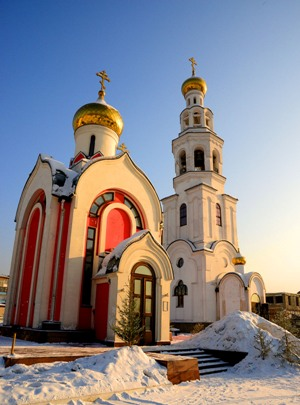
\includegraphics[width= 1\linewidth]{4a}
		\caption{\small\textit{\color{quantoan}Nhà thờ Phục sinh ở Kyzyl, Tuva (ảnh từ Internet).}}
%		\vspace*{-10pt}
	\end{figure}
\end{multicols}
\vspace*{-10pt}
{\rule{1\linewidth}{0.1pt}}
\vskip 0.25cm
\centerline{\LARGE\textbf{\color{quantoan}LỜI GIẢI, ĐÁP ÁN}}
\begin{multicols}{2}
	\textbf{\color{quantoan}Tìm ra người đặc biệt}
	\vskip 0.1cm
	$a)$ Ta sẽ chỉ ra chiến thuật dẫn tới mục đích phát hiện ra nhân viên $Z$ sau đúng $(n-1)$ câu hỏi. Đầu tiên, Xuân Phong chọn hai người tuỳ ý là $A$ và $B$. Xuân Phong hỏi nhân viên $A$ câu hỏi: ``Anh có biết $B$  không?" Nếu câu trả lời là ``Có" thì $B$ không phải là $Z$. Còn nếu câu trả lời là ``Không" thì $A$ không phải là $Z$. Như vậy, với một câu hỏi được đưa ra thì một người sẽ loại ra, tiếp theo không cần phải hỏi anh ta và cũng không cần hỏi về anh ta nữa. Cứ tiếp tục kiểu như vậy, ta loại đi $(n-1)$ người sau khi hỏi $(n-1)$ câu hỏi. Còn lại đúng một người. Anh ta chính là nhân viên $Z$.
	\vskip 0.1cm
	$b)$ Ta sẽ chỉ ra Xuân Phong phải hỏi không ít hơn $(n-1)$ câu hỏi. 
	\vskip 0.1cm
	Giả sử tại một bước nào đó của cuộc điều tra, Xuân Phong hỏi một nhân viên $A$, anh ta có biết nhân viên $B$ hay không. Trong trường hợp câu trả lời ``có", ta sẽ coi $B$ là được đánh dấu, còn trong trường hợp câu trả lời là ``không", ta sẽ coi $A$ là được đánh~dấu.
	\vskip 0.1cm
	\hfill (\textit{Xem tiếp trang} $64$)
\end{multicols}
%	\newpage
%
%	\thispagestyle{empty}
%	\begingroup 
%	\AddToShipoutPicture*{\put(0,0){\includegraphics[width=19.45cm]{Trian}}}
%	\centering
%	\vspace*{0cm}
%	\endgroup
%	\newpage	 
%	\pagestyle{empty}
%
	\setcounter{figure}{0}
	\thispagestyle{toancuabinone}
\pagestyle{toancuabi}
\everymath{\color{toancuabi}}
\blfootnote{$^*$\color{toancuabi}Nguồn: Câu lạc bộ Toán học Unicorn (UMC)}
\graphicspath{{../toancuabi/pic/}}
\begingroup
\AddToShipoutPicture*{\put(0,616){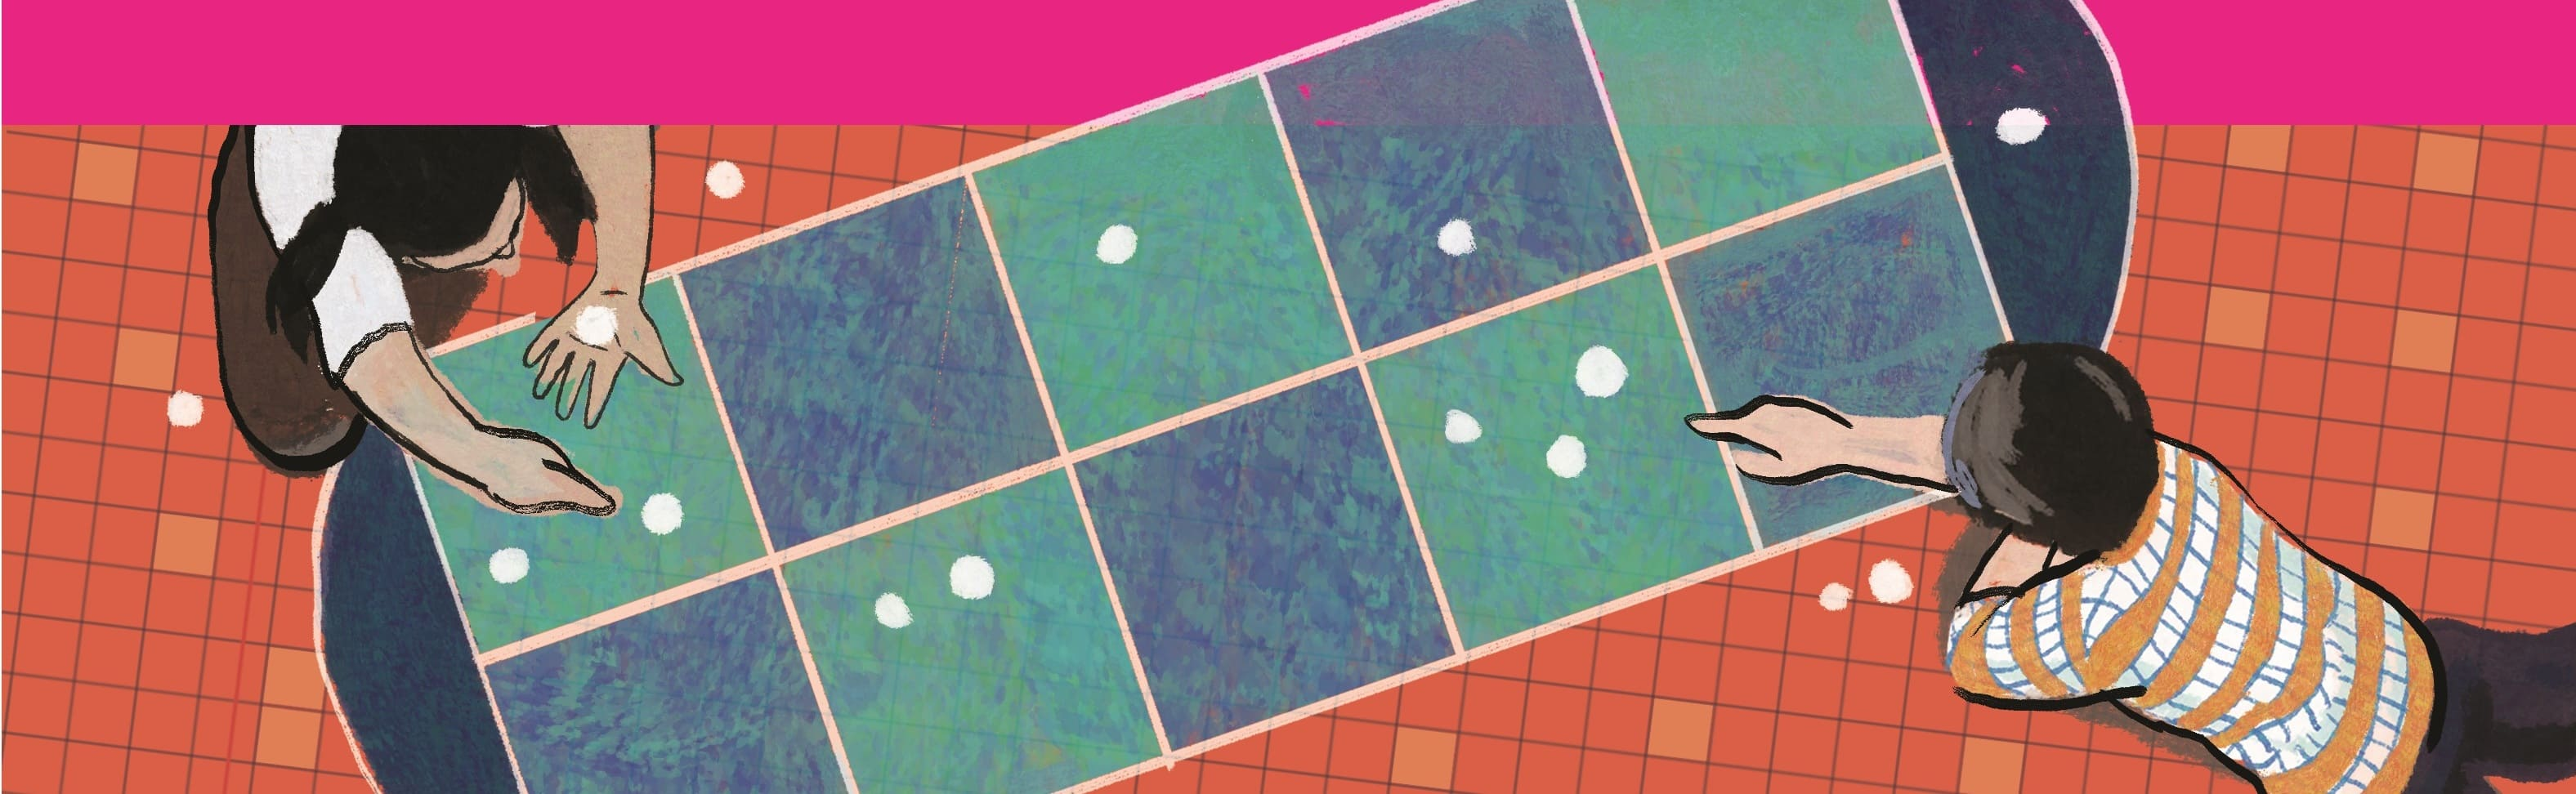
\includegraphics[width=19.3cm]{../bannertoancuabi}}}  
\AddToShipoutPicture*{\put(62,512){
\includegraphics[scale=1]{../tieude1.pdf}}}  
\centering
\endgroup
\vspace*{195pt} 

\definecolor{bulgarianrose}{rgb}{0.28, 0.02, 0.03}
\begin{multicols}{2}
	Trong số này, tạp chí Pi tiếp tục giới thiệu đến với bạn đọc đề thi tuyển sinh năm $2023-2024$ dành cho các bạn học sinh lớp $5$. Các bạn có thể thử sức làm của mình trong khoảng thời gian $90$ phút.
	\vskip 0.1cm
	\textbf{\color{toancuabi}Bài $\pmb1$.} 
	Dựa vào quy luật, hãy cho biết có bao nhiêu dấu thăng trong hình thứ tám của dãy hình sau.
	\begin{figure}[H]
		\vspace*{-5pt}
		\centering
		\captionsetup{labelformat= empty, justification=centering}
		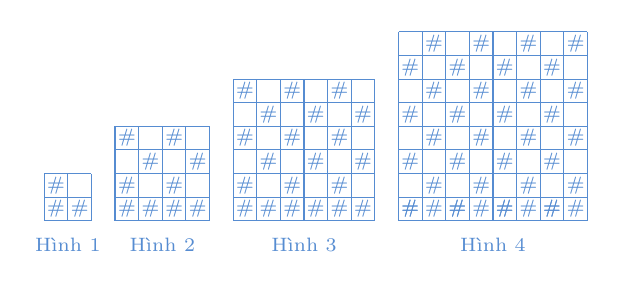
\begin{tikzpicture}[cackithi,scale=0.3,node font=\scriptsize]
			\draw (0,0) grid (2,2);	
			\draw (3,0) grid (7,4);
			\draw (8,0) grid (14,6);
			\draw (15,0) grid (23,8);
			\draw (0.5,0.5) node {$\#$};
			\draw (1.5,0.5) node {$\#$};
			\draw (0.5,1.5) node {$\#$};
			\draw (3.5,0.5) node {$\#$};
			\draw (4.5,0.5) node {$\#$};
			\draw (5.5,0.5) node {$\#$};
			\draw (6.5,0.5) node {$\#$};
			\draw (3.5,1.5) node {$\#$};
			\draw (5.5,1.5) node {$\#$};
			\draw (4.5,2.5) node {$\#$};
			\draw (6.5,2.5) node {$\#$};
			\draw (3.5,3.5) node {$\#$};
			\draw (5.5,3.5) node {$\#$};
			\draw (8.5,0.5) node {$\#$};
			\draw (9.5,0.5) node {$\#$};
			\draw (10.5,0.5) node {$\#$};
			\draw (11.5,0.5) node {$\#$};
			\draw (12.5,0.5) node {$\#$};
			\draw (13.5,0.5) node {$\#$};
			\draw (8.5,1.5) node {$\#$};
			\draw (10.5,1.5) node {$\#$};
			\draw (12.5,1.5) node {$\#$};
			\draw (9.5,2.5) node {$\#$};
			\draw (11.5,2.5) node {$\#$};
			\draw (13.5,2.5) node {$\#$};
			\draw (8.5,3.5) node {$\#$};
			\draw (10.5,3.5) node {$\#$};
			\draw (12.5,3.5) node {$\#$};
			\draw (9.5,4.5) node {$\#$};
			\draw (11.5,4.5) node {$\#$};
			\draw (13.5,4.5) node {$\#$};
			\draw (8.5,5.5) node {$\#$};
			\draw (10.5,5.5) node {$\#$};
			\draw (12.5,5.5) node {$\#$};
			\draw (15.5,0.5) node {$\#$};
			\draw (16.5,0.5) node {$\#$};
			\draw (17.5,0.5) node {$\#$};
			\draw (18.5,0.5) node {$\#$};
			\draw (19.5,0.5) node {$\#$};
			\draw (20.5,0.5) node {$\#$};
			\draw (21.5,0.5) node {$\#$};
			\draw (22.5,0.5) node {$\#$};
			\draw (15.5,0.5) node {$\#$};
			\draw (17.5,0.5) node {$\#$};
			\draw (19.5,0.5) node {$\#$};
			\draw (21.5,0.5) node {$\#$};
			\draw (16.5,1.5) node {$\#$};
			\draw (18.5,1.5) node {$\#$};
			\draw (20.5,1.5) node {$\#$};
			\draw (22.5,1.5) node {$\#$};
			\draw (15.5,2.5) node {$\#$};
			\draw (17.5,2.5) node {$\#$};
			\draw (19.5,2.5) node {$\#$};
			\draw (21.5,2.5) node {$\#$};
			\draw (16.5,3.5) node {$\#$};
			\draw (18.5,3.5) node {$\#$};
			\draw (20.5,3.5) node {$\#$};
			\draw (22.5,3.5) node {$\#$};
			\draw (15.5,4.5) node {$\#$};
			\draw (17.5,4.5) node {$\#$};
			\draw (19.5,4.5) node {$\#$};
			\draw (21.5,4.5) node {$\#$};
			\draw (16.5,5.5) node {$\#$};
			\draw (18.5,5.5) node {$\#$};
			\draw (20.5,5.5) node {$\#$};
			\draw (22.5,5.5) node {$\#$};
			\draw (15.5,6.5) node {$\#$};
			\draw (17.5,6.5) node {$\#$};
			\draw (19.5,6.5) node {$\#$};
			\draw (21.5,6.5) node {$\#$};
			\draw (16.5,7.5) node {$\#$};
			\draw (18.5,7.5) node {$\#$};
			\draw (20.5,7.5) node {$\#$};
			\draw (22.5,7.5) node {$\#$};
			\draw (1,-1) node {Hình $1$};
			\draw (5,-1) node {Hình $2$};
			\draw (11,-1) node {Hình $3$};
			\draw (19,-1) node {Hình $4$};
		\end{tikzpicture}
		\vspace*{-15pt}
	\end{figure}
	\textbf{\color{toancuabi}Bài $\pmb2$.} Bạn Tâm xếp các số $0, 0, 1, 1, 2, 2, 2, 3$ vào các ô vuông trong hình dưới đây (mỗi ô một số) để tạo thành phép trừ của hai số có $4$ chữ số. Hỏi hiệu nhận được lớn nhất có thể là bao nhiêu? 
	\vskip 0.1cm
	Chú ý: \textit{một số có bốn chữ số không được bắt đầu bằng số $0$.}
	\begin{figure}[H]
		\vspace*{-5pt}
		\centering
		\captionsetup{labelformat= empty, justification=centering}
		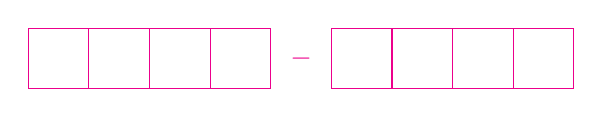
\begin{tikzpicture}[toancuabi,scale=0.77]
			\draw (0,0) grid (4,1);
			\draw (4.5,0.5) node {$-$};
			\draw (5,0) grid (9,1);
		\end{tikzpicture}
		\vspace*{-10pt}
	\end{figure}
	\textbf{\color{toancuabi}Bài $\pmb3$.} Diện tích của hình được tô đậm bên dưới bằng bao nhiêu?
	\begin{figure}[H]
		\vspace*{5pt}
		\centering
		\captionsetup{labelformat= empty, justification=centering}
		\definecolor{zzttqq}{rgb}{0.6,0.2,0.}
		\begin{tikzpicture}[toancuabi, scale=0.9]
			\fill[color=cackithi,fill=cackithi!40] (1.,0.) -- (2.,5.) -- (3.,0.) -- cycle;
			\fill[color=zzttqq,fill=cackithi!40] (1.,0.) -- (4.,5.) -- (3.,0.) -- (0.,5.) -- cycle;
			\draw  (1.,0.)-- (2.,5.);
			\draw  (2.,5.)-- (3.,0.);
			\draw  (3.,0.)-- (1.,0.);
			\draw  (1.,0.)-- (4.,5.);
			\draw  (4.,5.)-- (3.,0.);
			\draw  (3.,0.)-- (0.,5.);
			\draw  (0.,5.)-- (1.,0.);
			\draw[dashed]  (-1.,5.)-- (5.,5.);
			\draw[dashed]  (-1.,2.5)-- (5.,2.5);
			\draw[dashed]  (-1.,0.)-- (5.,0.);
			\draw[-stealth]  (4.5,5.)-- (4.5,2.5);
			\draw[-stealth]  (4.5,2.5)-- (4.5,0.);
			\draw[-stealth]  (1,-0.4)-- (3.,-0.4);
			
			\draw[-stealth]  (4.5,2.5) -- (4.5,5.);
			\draw[-stealth]  (4.5,0.) -- (4.5,2.5);
			\draw[-stealth]  (3.,-0.4) -- (1,-0.4);
			\draw[color=black] (4.21498164902576,3.87946061896495) node {$5$};
			\draw[color=black] (4.143071467449243,1.3626042637868525) node {$5$};
			\draw[color=black] (2.039698656336115,-0.709930933849792) node {$4$};
		\end{tikzpicture}
		\vspace*{-10pt}
	\end{figure}
	\textbf{\color{toancuabi}Bài $\pmb4$.} Trong bảng ô vuông cỡ $4\times 4$ có điền các số khác $0$ sao cho tích của $4$ số trong mỗi hàng, mỗi cột đều bằng nhau. Cho biết các số trong $9$ ô như hình vẽ, hỏi số ở ô có dấu $*$ bằng bao nhiêu?
	\begin{figure}[H]
		\vspace*{-5pt}
		\centering
		\captionsetup{labelformat= empty, justification=centering}
		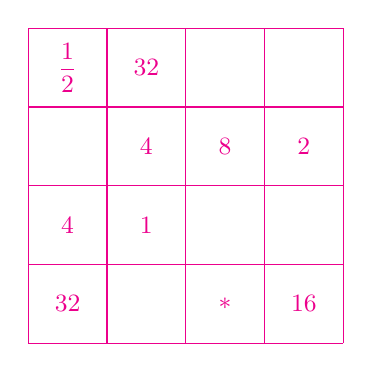
\begin{tikzpicture}[toancuabi, node font=\small]
			\draw (0,0) grid (4,4);
			\draw (0.5,0.5) node {$32$};
			\draw (0.5,1.5) node {$4$};
			\draw (0.5,3.5) node {$\dfrac{1}{2}$};
			\draw (1.5,1.5) node {$1$};
			\draw (1.5,2.5) node {$4$};
			\draw (1.5,3.5) node {$32$};
			\draw (2.5,0.5) node {$*$};
			\draw (3.5,0.5) node {$16$};
			\draw (2.5,2.5) node {$8$};
			\draw (3.5,2.5) node {$2$};
		\end{tikzpicture}
		\vspace*{-5pt}
	\end{figure}
	\textbf{\color{toancuabi}Bài $\pmb5$.} Khu vườn của gia đình Tâm được minh họa bằng hình chữ nhật trong hình dưới đây. Biết rằng khu vườn có diện tích $120 \,m^2$ và được chia thành ba luống hình chữ nhật. Phần trồng hoa rộng $2\,m$, diện tích $20 \,m^2$, phần trồng dâu rộng $3\, m$. Hỏi diện tích phần trồng rau là bao nhiêu?
	\begin{figure}[H]
		\vspace*{-5pt}
		\centering
		\captionsetup{labelformat= empty, justification=centering}
		\begin{tikzpicture}[scale=0.4,toancuabi]
			\draw (0,0) rectangle (12,10);
			\draw (2,0) -- (2,10) (2,3) -- (12,3);
			\draw (1,10) node[below] {$2\,m$};
			\draw (1,5) node {Hoa};
			\draw (7,1.5) node {Dâu};
			\draw (7,6.5) node {Rau};
			\draw (12,1.5) node[right] {$3\,m$};
		\end{tikzpicture}
		\vspace*{-5pt}
	\end{figure}
	\textbf{\color{toancuabi}Bài $\pmb6$.} Ba bạn An, Bình, Chi chia đều nhau $30$ chiếc kẹo. An ăn một số chiếc kẹo; Bình ăn một số kẹo bằng với số kẹo mà An còn; Chi ăn số kẹo bằng với tổng số kẹo mà An và Bình đã ăn. Hỏi còn lại bao nhiêu chiếc kẹo?
	\vskip 0.1cm
	\textbf{\color{toancuabi}Bài $\pmb7$.} Một bác nông dân chở một xe ô tô quất cảnh ra chợ Tết để bán. Sau khi bán hết cây quất cuối cùng với giá $230$ nghìn đồng, bác tính nhẩm lại thấy mình đã bán số cây quất với giá trung bình là $245$ nghìn đồng/cây. Nhưng người mua cây quất cuối quay trở lại và chỉ cho bác thấy cành quất bị rụng quá nhiều lá, nên ông ta chỉ đồng ý mua với giá $158$ nghìn đồng. Bác chấp thuận và bán cây quất đó. Khi nhẩm tính lại, bác nông dân thấy giá trung bình của xe quất bây giờ là $242$ nghìn đồng. Hỏi bác đã bán được bao nhiêu cây quất?
	\vskip 0.1cm
	\columnbreak
	\textbf{\color{toancuabi}Bài $\pmb8$.} Có bao nhiêu cách xếp $5$ viên bi giống hệt nhau vào các ô hình vuông ở hình vẽ sau sao cho mỗi ô có không quá $1$ viên bi và không có $2$ viên bi nào trên cùng $1$ hàng hoặc $1$ cột?
	\begin{figure}[H]
		\vspace*{-10pt}
		\centering
		\captionsetup{labelformat= empty, justification=centering}
		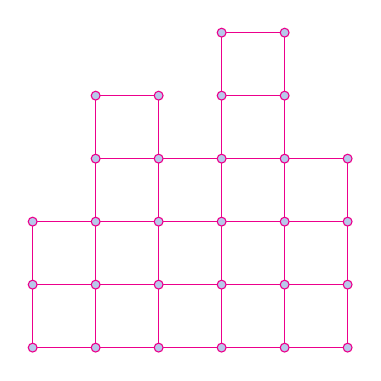
\begin{tikzpicture}[toancuabi,scale=0.8]
			\draw  (0.,1.)-- (5.,1.);
			\draw  (5.,1.)-- (5.,4.);
			\draw  (5.,4.)-- (1.,4.);
			\draw  (1.,4.)-- (1.,3.);
			\draw  (1.,3.)-- (0.,3.);
			\draw  (0.,3.)-- (0.,1.);
			\draw  (1.,1.)-- (1.,3.);
			\draw  (1.,2.)-- (5.,2.);
			\draw  (5.,3.)-- (1.,3.);
			\draw  (1.,4.)-- (1.,5.);
			\draw  (1.,5.)-- (2.,5.);
			\draw  (2.,5.)-- (2.,1.);
			\draw  (3.,1.)-- (3.,6.);
			\draw  (3.,6.)-- (4.,6.);
			\draw  (4.,6.)-- (4.,1.);
			\draw  (0.,2.)-- (1.,2.);
			\draw  (3.,5.)-- (4.,5.);
			
			\draw [fill=cackithi!40] (0.,1.) circle (2.0pt);
			\draw [fill=cackithi!40] (5.,1.) circle (2.0pt);
			\draw [fill=cackithi!40] (5.,4.) circle (2.0pt);
			\draw [fill=cackithi!40] (1.,4.) circle (2.0pt);
			\draw [fill=cackithi!40] (1.,3.) circle (2.0pt);
			\draw [fill=cackithi!40] (0.,3.) circle (2.0pt);
			\draw [fill=cackithi!40] (1.,1.) circle (2.0pt);
			\draw [fill=cackithi!40] (1.,2.) circle (2.0pt);
			\draw [fill=cackithi!40] (5.,2.) circle (2.0pt);
			\draw [fill=cackithi!40] (5.,3.) circle (2.0pt);
			\draw [fill=cackithi!40] (1.,5.) circle (2.0pt);
			\draw [fill=cackithi!40] (2.,5.) circle (2.0pt);
			\draw [fill=cackithi!40] (2.,1.) circle (2.0pt);
			\draw [fill=cackithi!40] (3.,1.) circle (2.0pt);
			\draw [fill=cackithi!40] (3.,6.) circle (2.0pt);
			\draw [fill=cackithi!40] (4.,6.) circle (2.0pt);
			\draw [fill=cackithi!40] (4.,1.) circle (2.0pt);
			\draw [fill=cackithi!40] (2.,4.) circle (2.0pt);
			\draw [fill=cackithi!40] (3.,4.) circle (2.0pt);
			\draw [fill=cackithi!40] (4.,4.) circle (2.0pt);
			\draw [fill=cackithi!40] (4.,5.) circle (2.0pt);
			\draw [fill=cackithi!40] (3.,5.) circle (2.0pt);
			\draw [fill=cackithi!40] (4.,3.) circle (2.0pt);
			\draw [fill=cackithi!40] (3.,3.) circle (2.0pt);
			\draw [fill=cackithi!40] (2.,3.) circle (2.0pt);
			\draw [fill=cackithi!40] (2.,2.) circle (2.0pt);
			\draw [fill=cackithi!40] (3.,2.) circle (2.0pt);
			\draw [fill=cackithi!40] (4.,2.) circle (2.0pt);
			\draw [fill=cackithi!40] (0.,2.) circle (2.0pt);
		\end{tikzpicture}
		\vspace*{-5pt}
	\end{figure}
	\textbf{\color{toancuabi}Bài $\pmb9$.} Mỗi ô trong hình bên được điền một số sao cho: số được ghi trong mỗi ô ở $3$ hàng trên cùng bằng tổng $2$ số ở hai ô ngay bên dưới nó. 
	Cho biết trước $3$ số như trong hình vẽ, hỏi số nào phải được điền vào ô có chữ $x$?
	\begin{figure}[H]
		\vspace*{-5pt}
		\centering
		\captionsetup{labelformat= empty, justification=centering}
		\begin{tikzpicture}[xscale=2,scale=0.8,toancuabi]
			\draw (0,0) grid (4,1);
			\draw (1,2) grid (3,3);
			\draw (0.5,1) rectangle (3.5,2);
			\draw (1.5,3) rectangle (2.5,4);
			\draw (1.5,1) --(1.5,2) (2.5,1) --(2.5,2);
			\draw (0.5,0.5) node {$10$};
			\draw (3.5,0.5) node {$12$};
			\draw (2,1.5) node {$x$};
			\draw (2,3.5) node {$100$};
		\end{tikzpicture}
		\vspace*{-5pt}
	\end{figure}
	\textbf{\color{toancuabi}Bài $\pmb{10}$.} Sau khi sạc điện thoại di động, bạn Kiên nhận ra mình đã quên mã PIN (mã gồm $4$ chữ số). Kiên nhớ là mã PIN bắt đầu bằng số $1$, kết thúc bằng số $3$ và các chữ số trong mã đều khác nhau.
	Có bao nhiêu số khác nhau cho mã PIN của Kiên?
	\vskip 0.1cm
	\hfill\textit{Xem lời giải/đáp án trang $20$} 
\end{multicols}
\newpage
\graphicspath{{../toancuabi/pic/}}
\begingroup
\AddToShipoutPicture*{\put(122,680){
\includegraphics[scale=1]{../tieude.pdf}}}  
\centering
\endgroup
\vspace*{25pt} 
\begin{multicols}{2}
	Thám tử Xuân Phong phải cải trang thành một nhà báo để tìm hiểu về một công ty nước giải khát có uy tín, tuy nhiên mới đây đã bất ngờ bị lộ bí mật về công thức pha chế với đối thủ cạnh tranh. Trong vai trò của một nhà báo, Xuân Phong tham gia một buổi họp đặc biệt gồm $n$ nhân viên chủ chốt của công ty. Xuân Phong được biết rằng, trong số $n$ người này có một người, có bí danh là Z, biết toàn bộ mọi nhân viên còn lại, tuy nhiên không một ai trong số $n-1$ người còn lại lại biết anh ta. Người có bí danh Z này có thể cho Xuân Phong đầu mối vì sao công thức pha chế bị lộ ra ngoài.
	\vskip 0.1cm
	Xuân Phong có thể tới cạnh mỗi một người bất kỳ trong buổi họp, và hỏi anh ta câu hỏi sau: ``Anh có biết <một người nào đó> không?" (trong ngoặc < > là một người cụ thể nào đó trong số những người còn lại). Rất may, khác với mọi lần, lần này  tất cả $n$ người đều nói thật, và Xuân Phong có thể hỏi một người nhiều hơn một lần.
	\vskip 0.1cm
	$a)$ Hỏi Xuân Phong có thể xác định được ai là Z sau khi đưa ra ít hơn $n$ câu hỏi được hay không?
	\vskip 0.1cm
	$b)$ Tìm số câu hỏi ít nhất đủ để Xuân Phong luôn tìm được nhân viên Z. Em hãy chứng minh rằng không thể hỏi ít hơn số câu hỏi như vậy được.
	\begin{figure}[H]
		\centering
		\vspace*{-10pt}
		\captionsetup{labelformat= empty, justification=centering}
		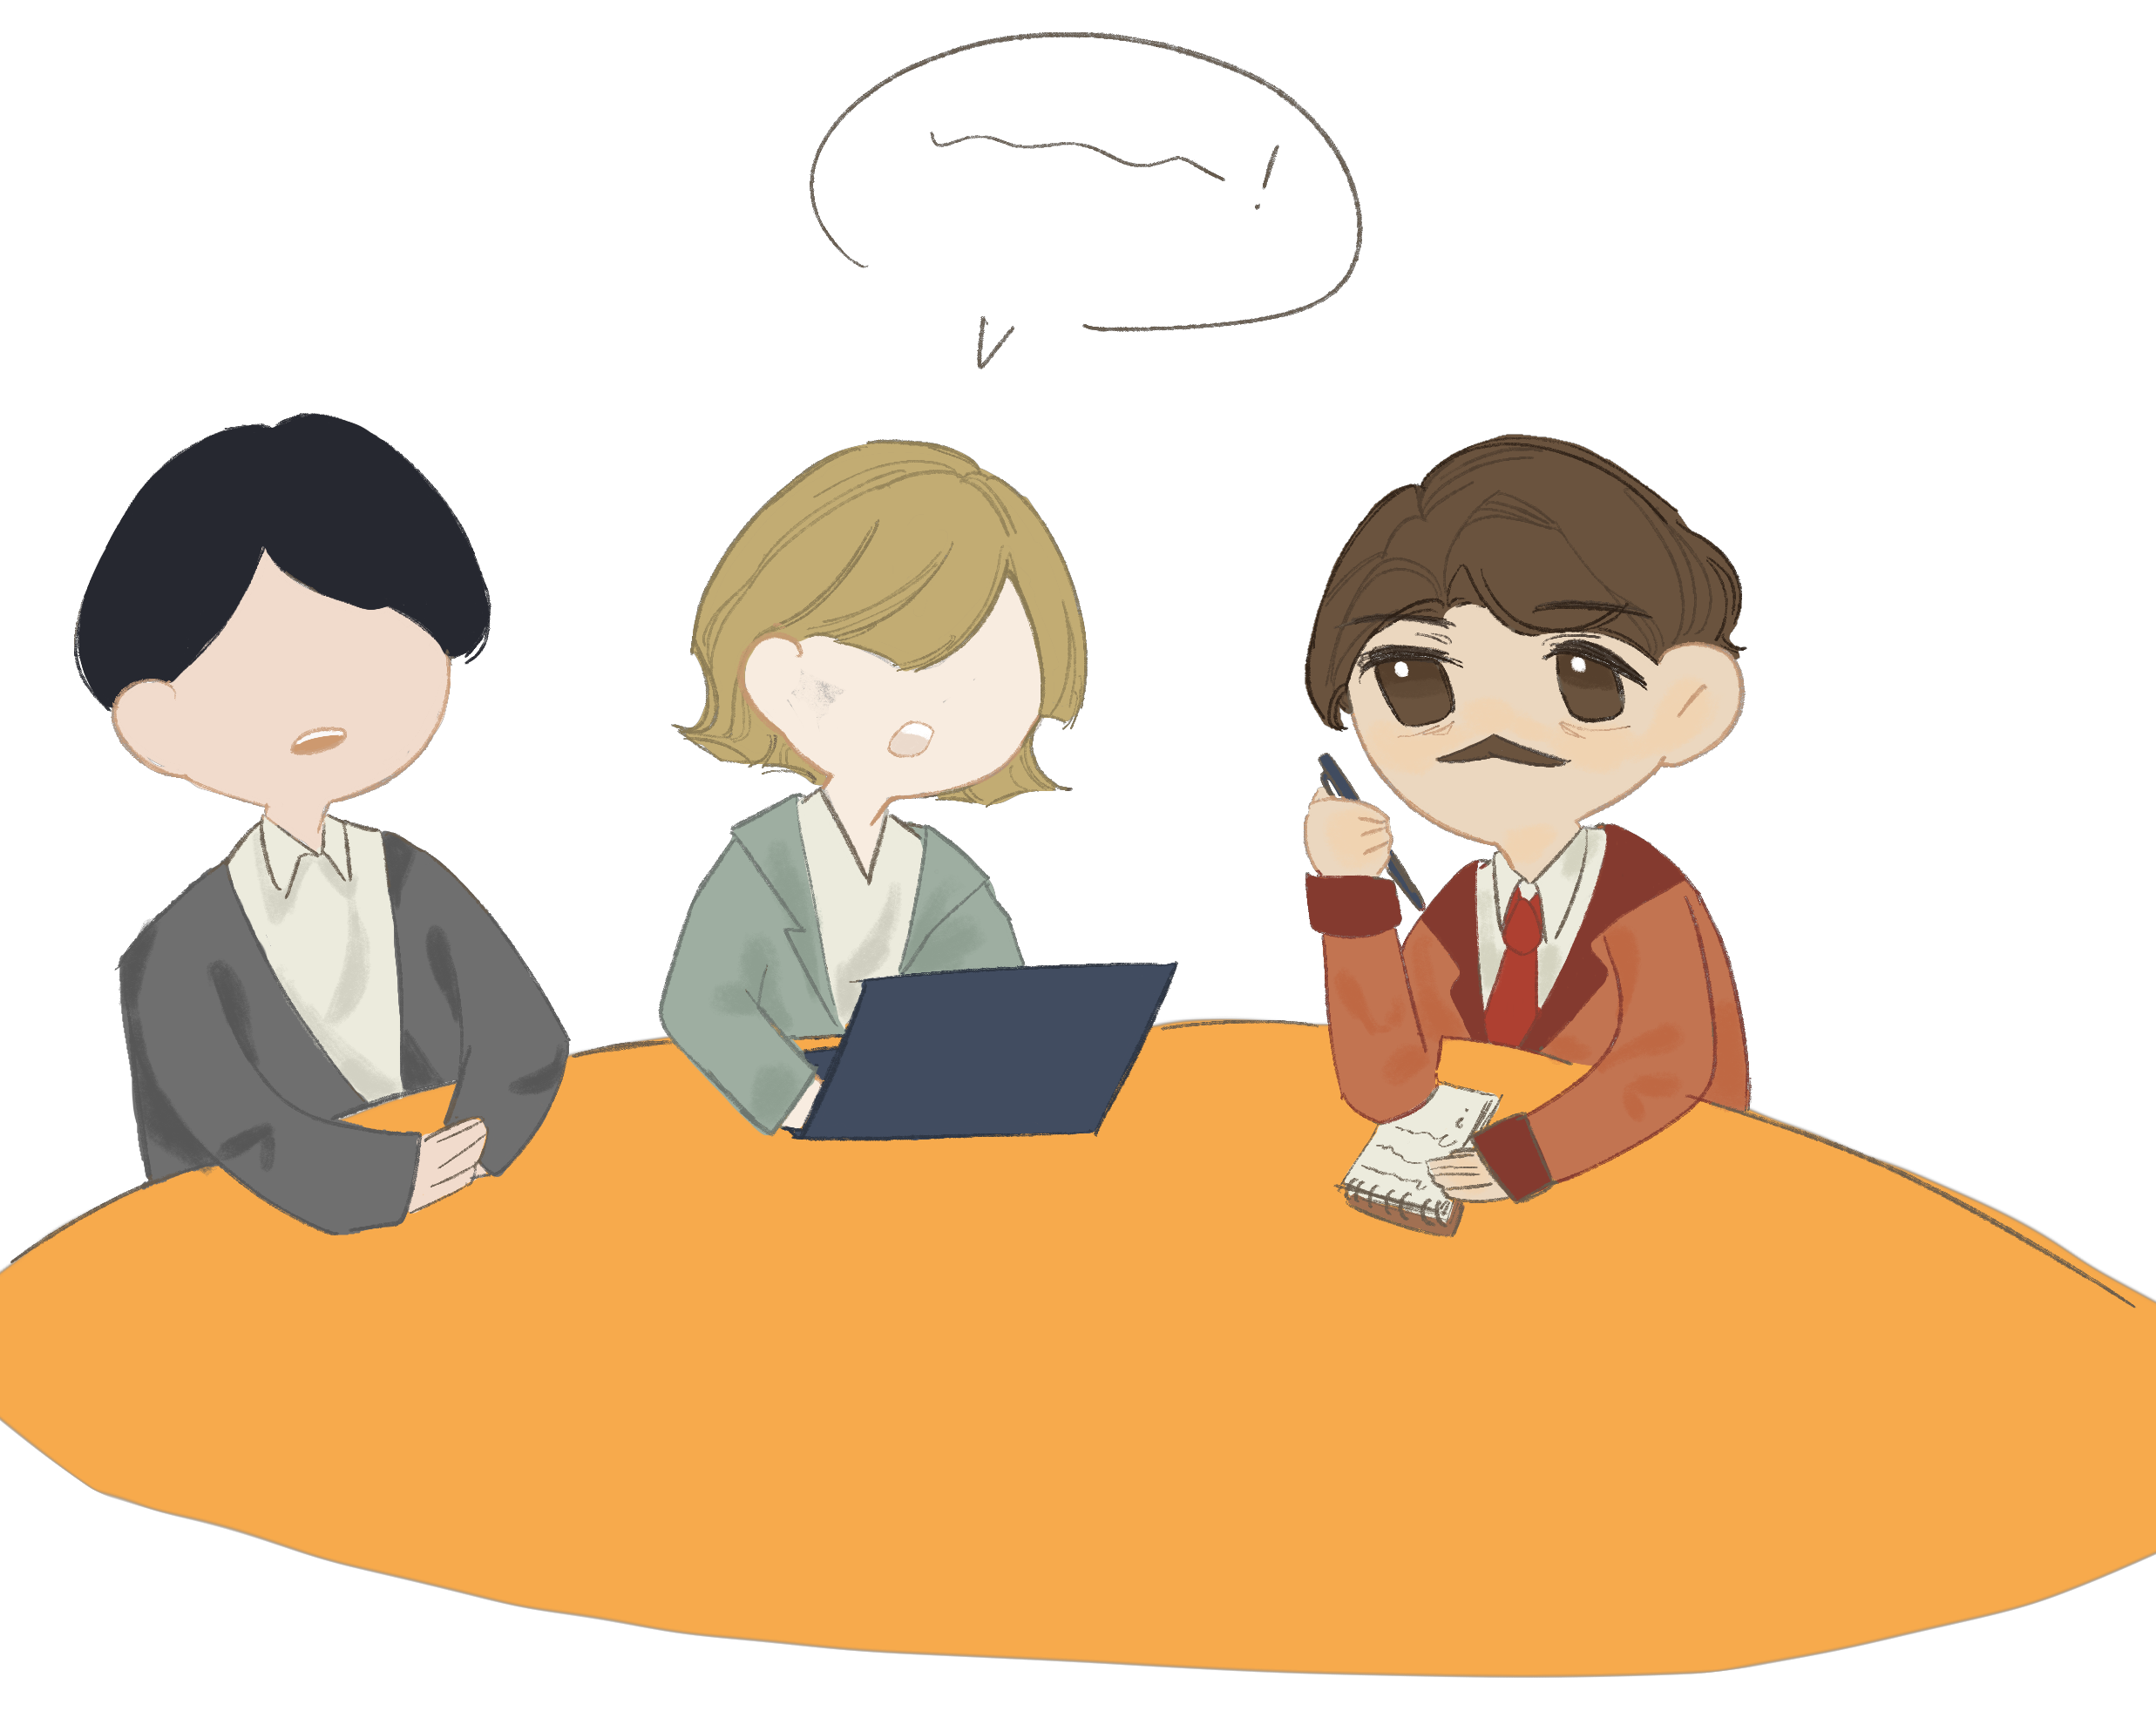
\includegraphics[width=0.95\linewidth]{xp}
		\vspace*{-5pt}
	\end{figure}
\end{multicols}
\vspace*{-10pt}
{\color{toancuabi}\rule{1\linewidth}{0.1pt}}

\begingroup
\AddToShipoutPicture*{\put(120,295){
\includegraphics[scale=1]{../tieude11.pdf}}} 
\centering
\endgroup
\vspace*{60pt}

\begin{multicols}{2}
	$\pmb{1.}$ Nàng Lọ Lem đi lạc vào trong rừng. Theo lời khuyên của bà tiên, nàng tìm thấy ba chiếc rương đựng những hạt dẻ có thể đem lại điều ước. Chiếc rương thứ nhất có ít hơn $6$ hạt dẻ
	\begin{figure}[H]
		\centering
		\vspace*{-5pt}
		\captionsetup{labelformat= empty, justification=centering}
		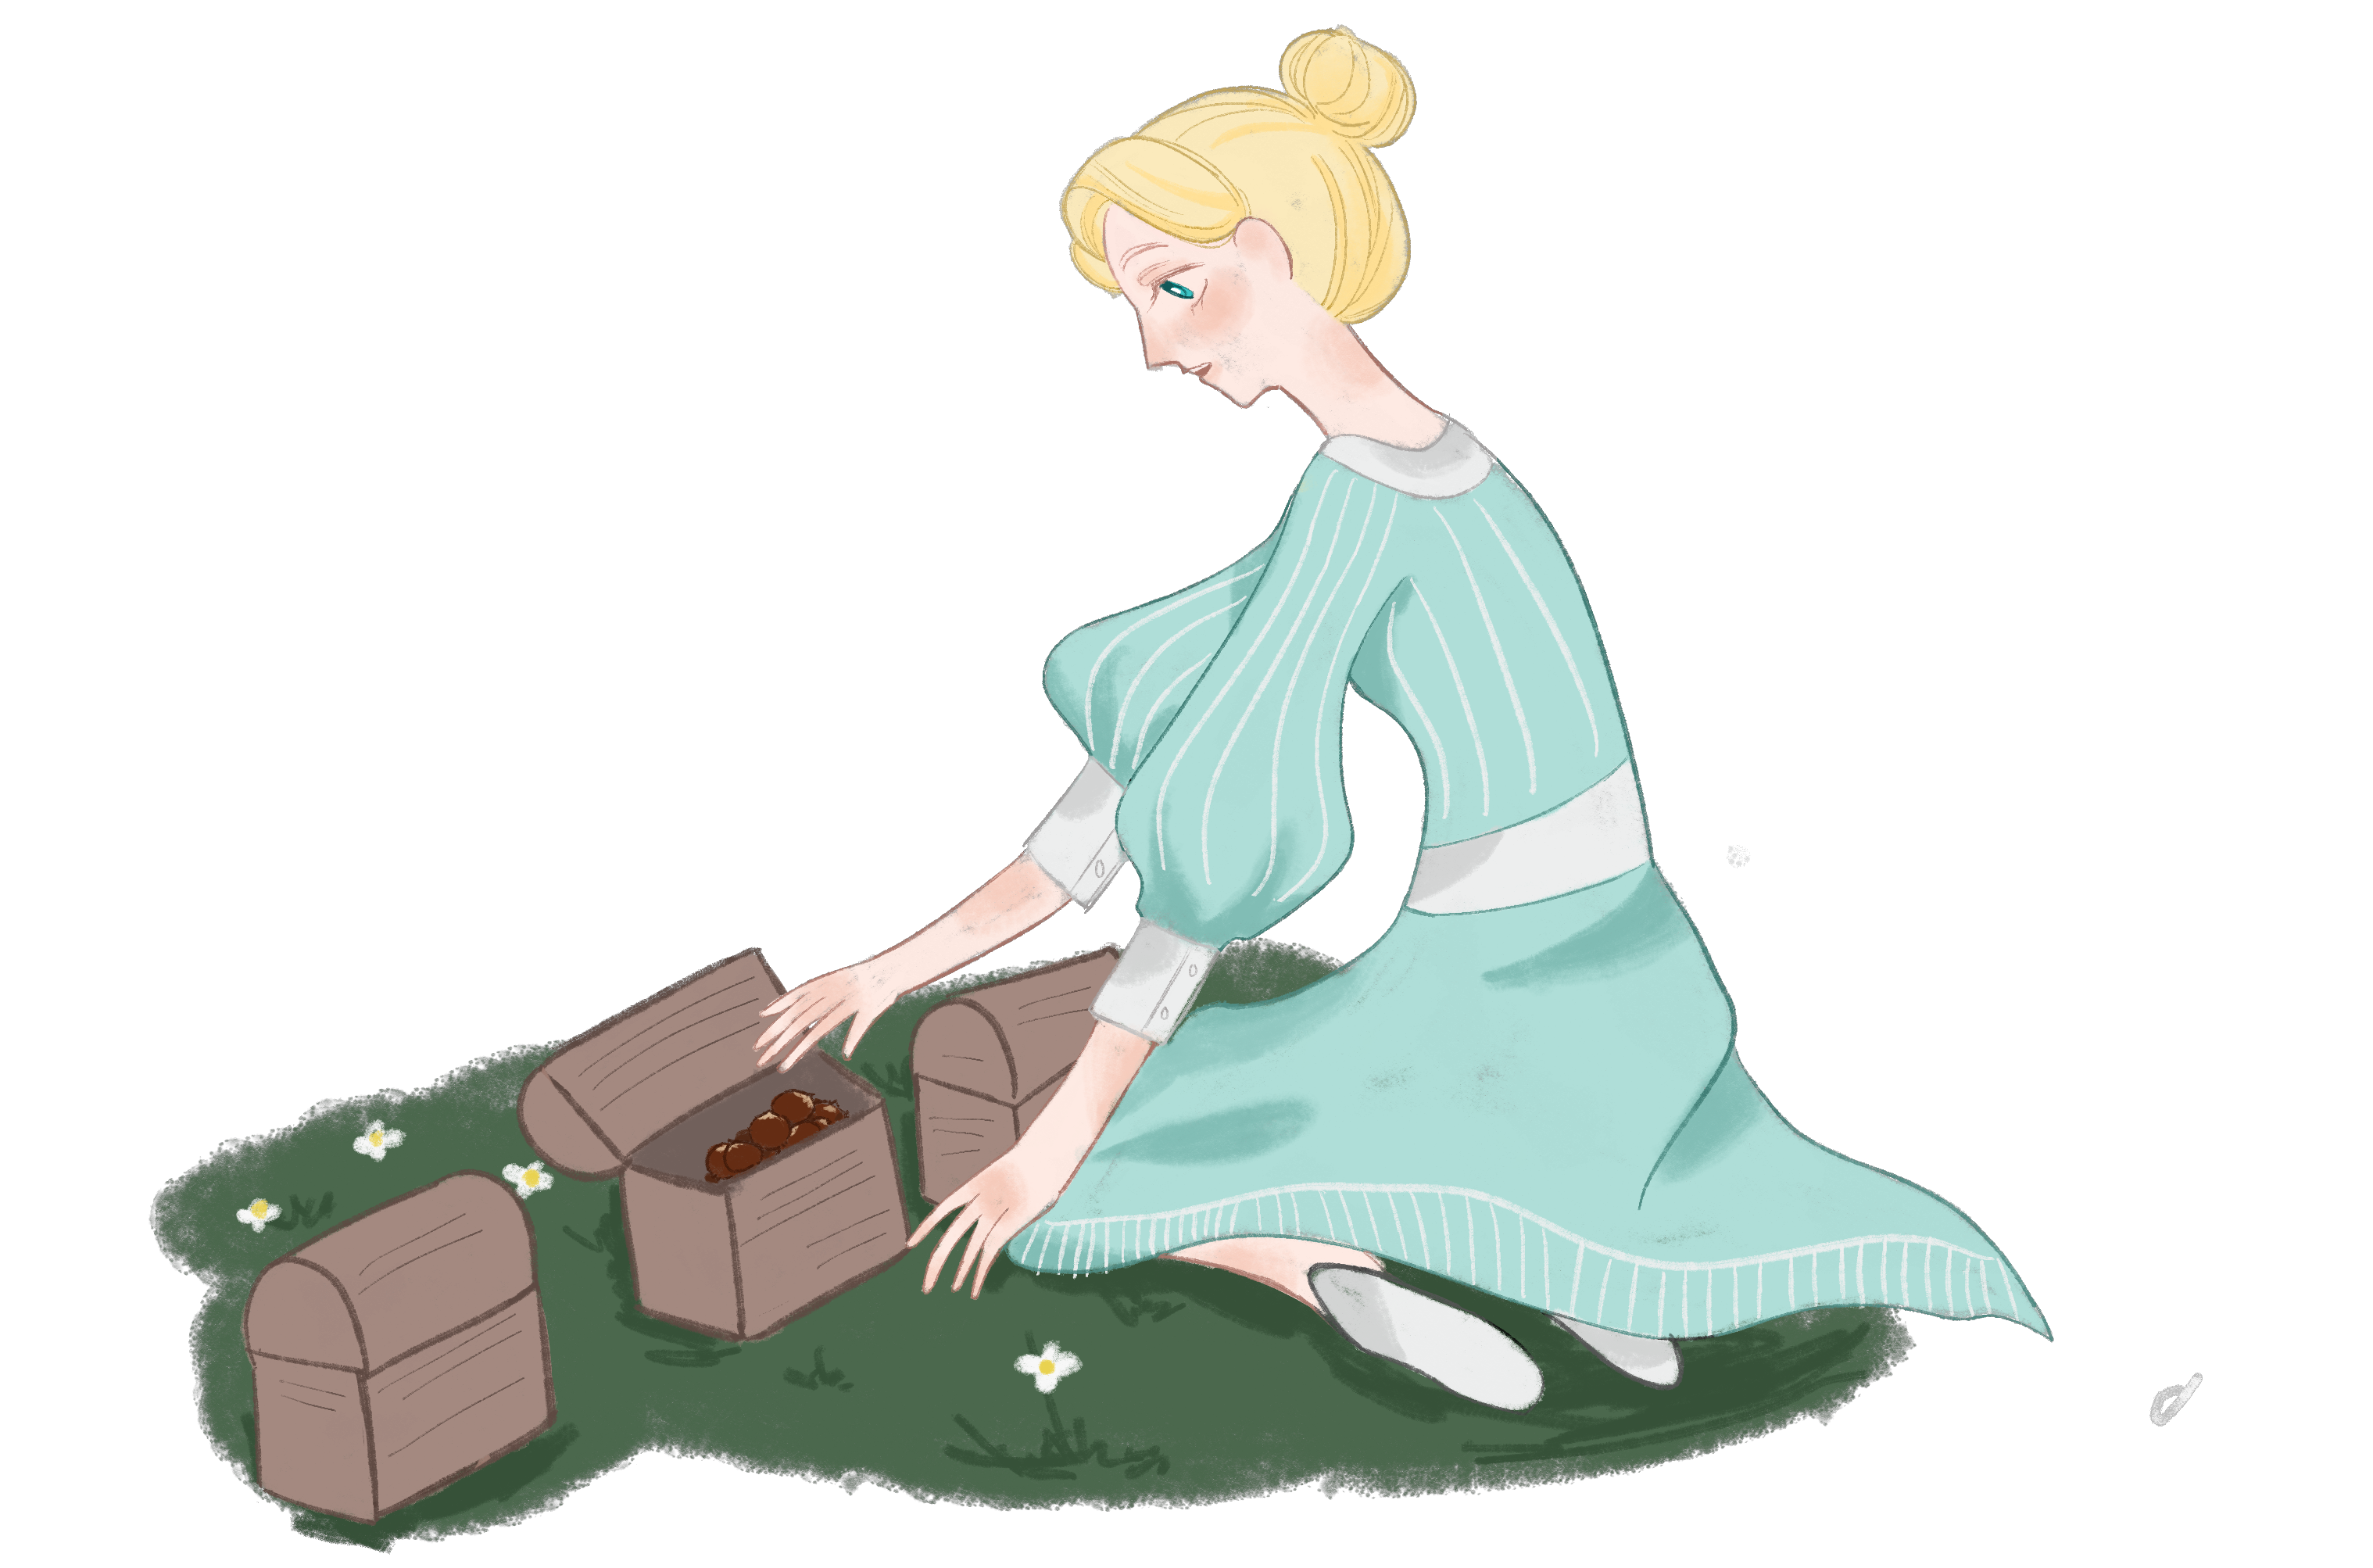
\includegraphics[width=1\linewidth]{Hinh1}
		\vspace*{-5pt}
	\end{figure}
	so với  tổng số hạt dẻ ở hai chiếc rương còn lại. Chiếc rương thứ hai có ít hơn $10$ hạt dẻ so với tổng số hạt dẻ ở chiếc rương thứ nhất và thứ ba. Hỏi trong chiếc rương thứ ba có bao nhiêu hạt dẻ?
	\vskip 0.1cm
	$\pmb{2.}$ Bạn Vân viết $150$ chữ số xung quanh một vòng tròn. Nếu đọc $150$ chữ số này theo chiều kim đồng hồ bắt đầu từ một chỗ nào đó bất kì, thì Vân thấy số nhận được chia hết cho $27$. Em hãy chứng minh rằng, nếu Vân bắt đầu từ bất kỳ một chỗ khác và đọc ngược chiều kim đồng hồ toàn bộ $150$ chữ số đã viết, thì bạn cũng nhận được một số chia hết cho $27$.
	\begin{figure}[H]
		\centering
%		\vspace*{-5pt}
		\captionsetup{labelformat= empty, justification=centering}
		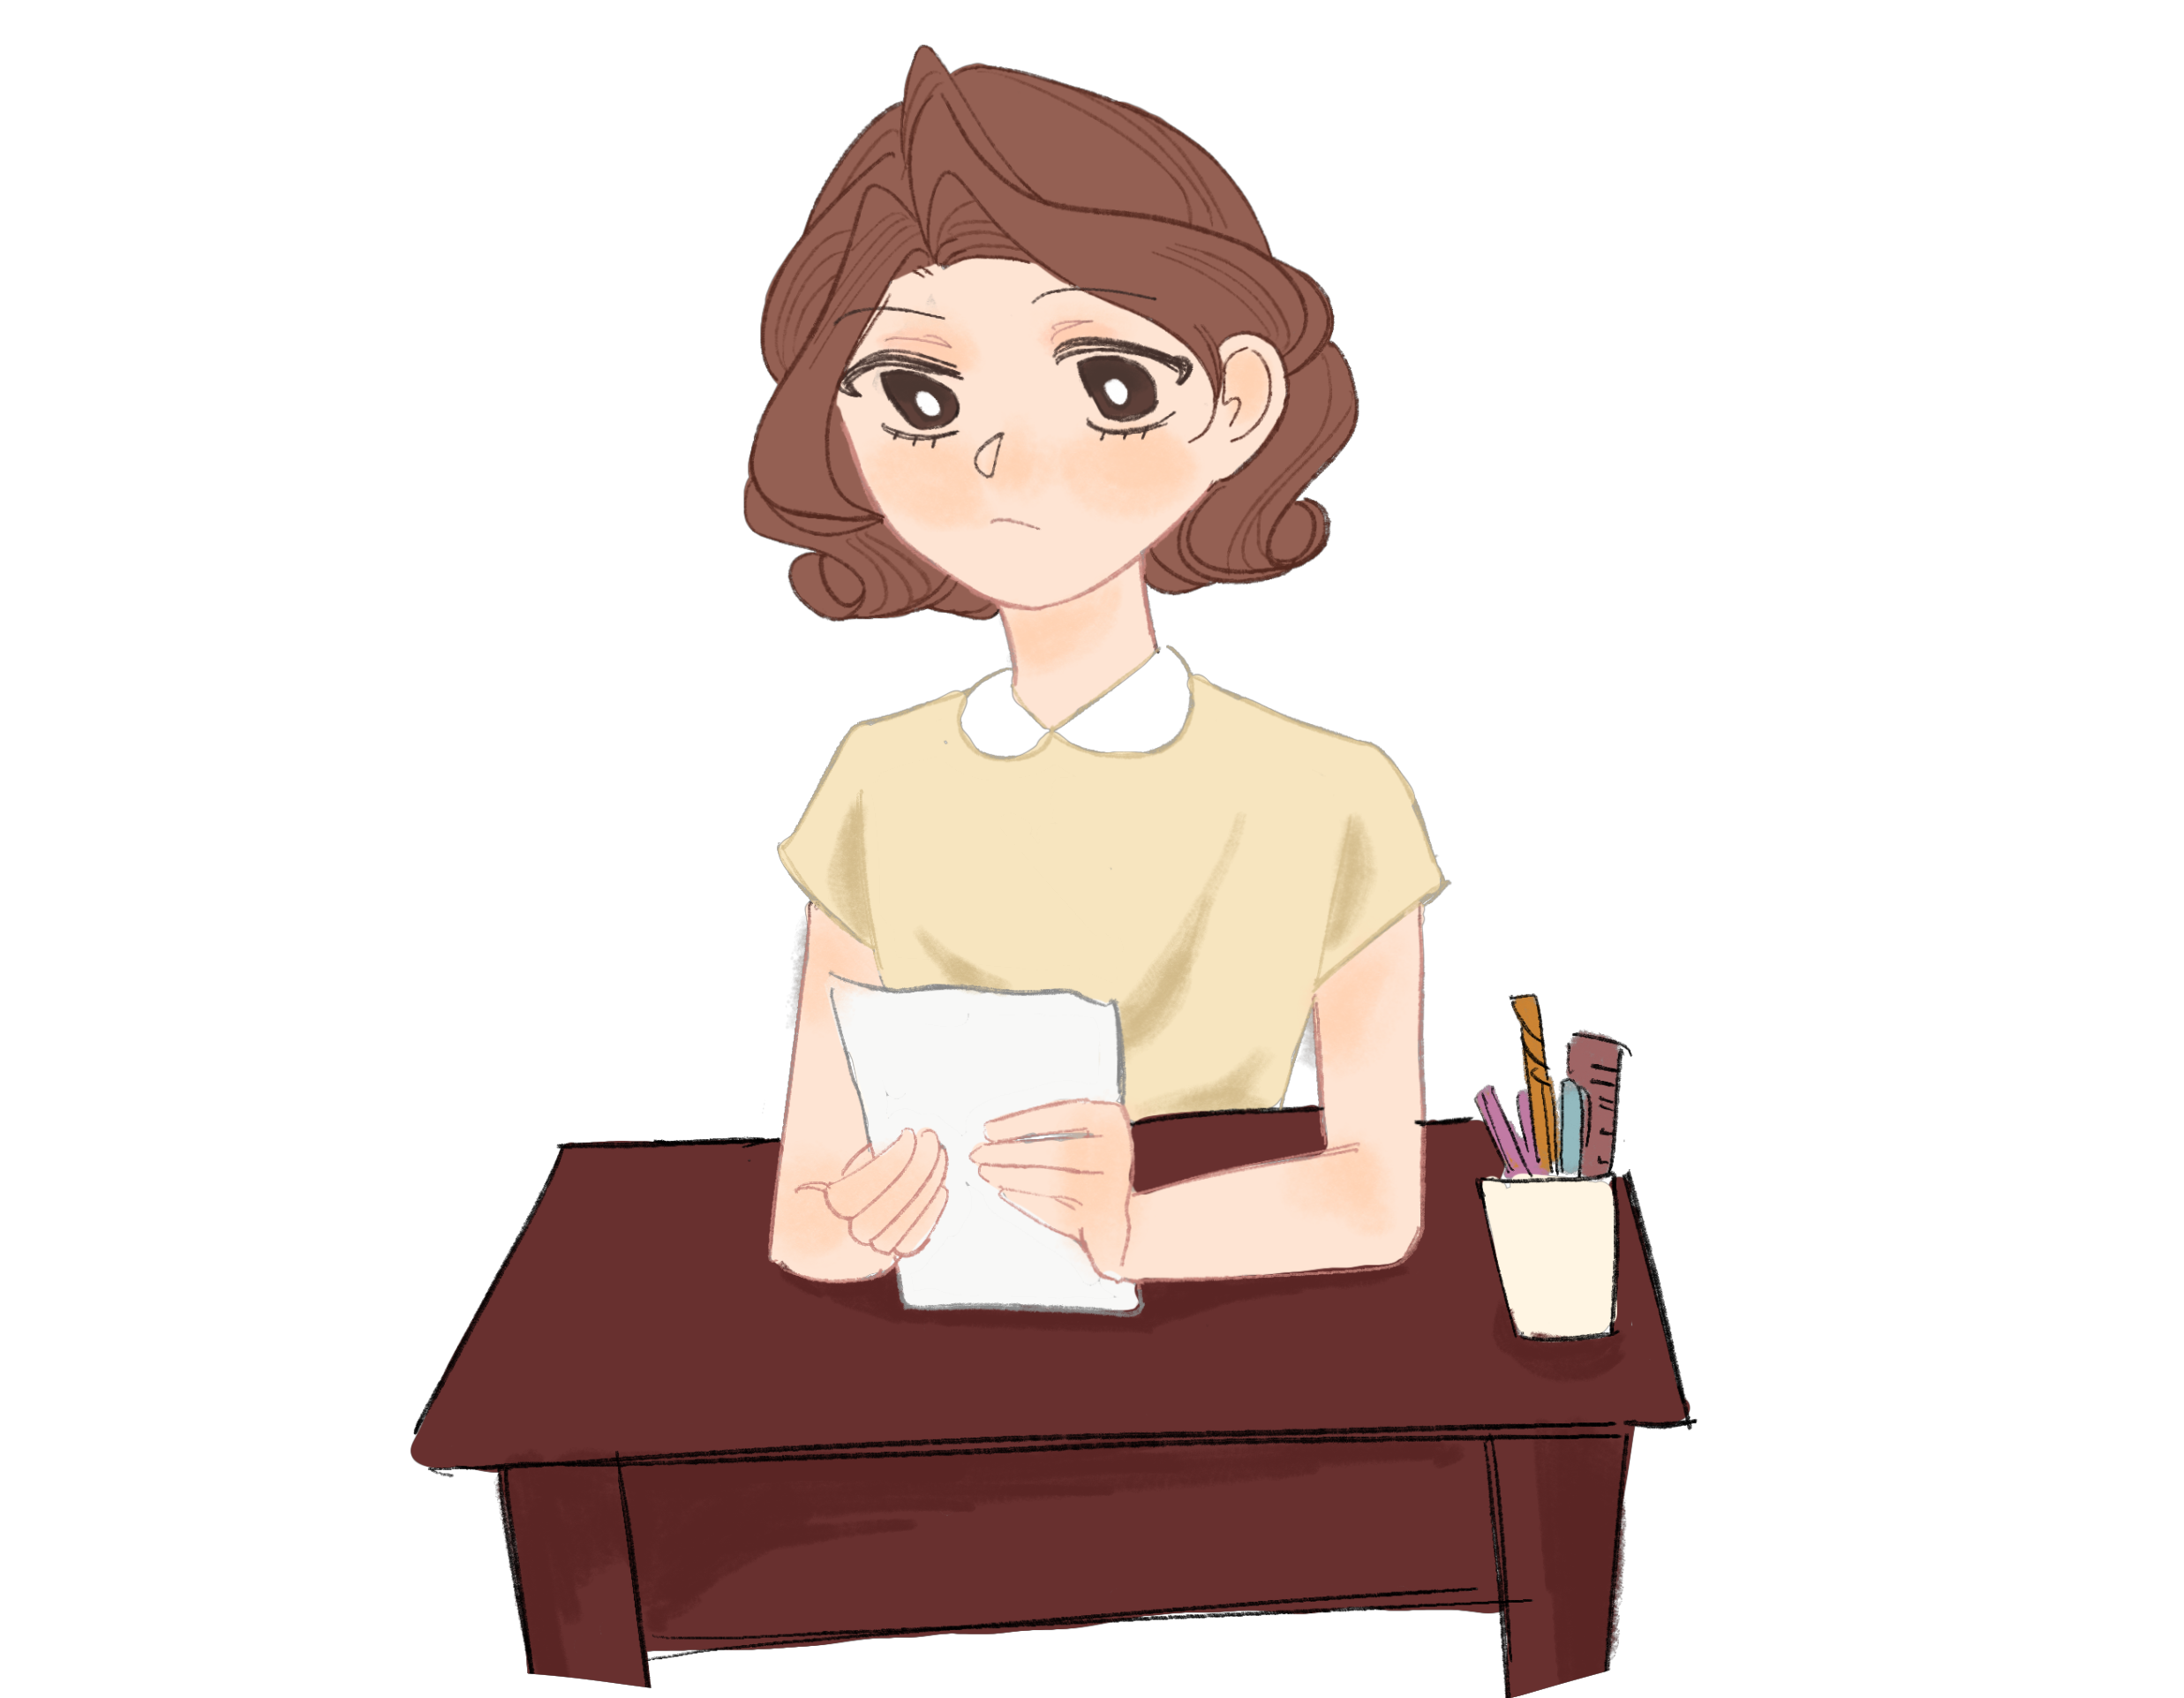
\includegraphics[width=0.85\linewidth]{Hinh2}
		\vspace*{-5pt}
	\end{figure}
	$\pmb{3.}$ Có ba tên cướp ăn trộm được $10$ viên kim cương trong một két sắt với tổng giá trị là $4 000 000$ dollar. Chúng dự định sẽ phân chia những viên kim cương này cho nhau để mỗi tên có được ít nhất $1 000 000$ dollar. Khi bị cảnh sát truy đuổi, một viên kim cương trị giá $600 000$ dollar bị rơi mất, và vì thế chúng không thể chia được những viên kim cương như dự định ban đầu. Hỏi ba tên cướp này có bị nhầm lẫn ở đâu không, hay là trước khi bị rơi viên kim cương, việc chia đồ ăn trộm của chúng đã không thể thực hiện được theo như dự định?
	\begin{figure}[H]
		\centering
		\vspace*{-5pt}
		\captionsetup{labelformat= empty, justification=centering}
		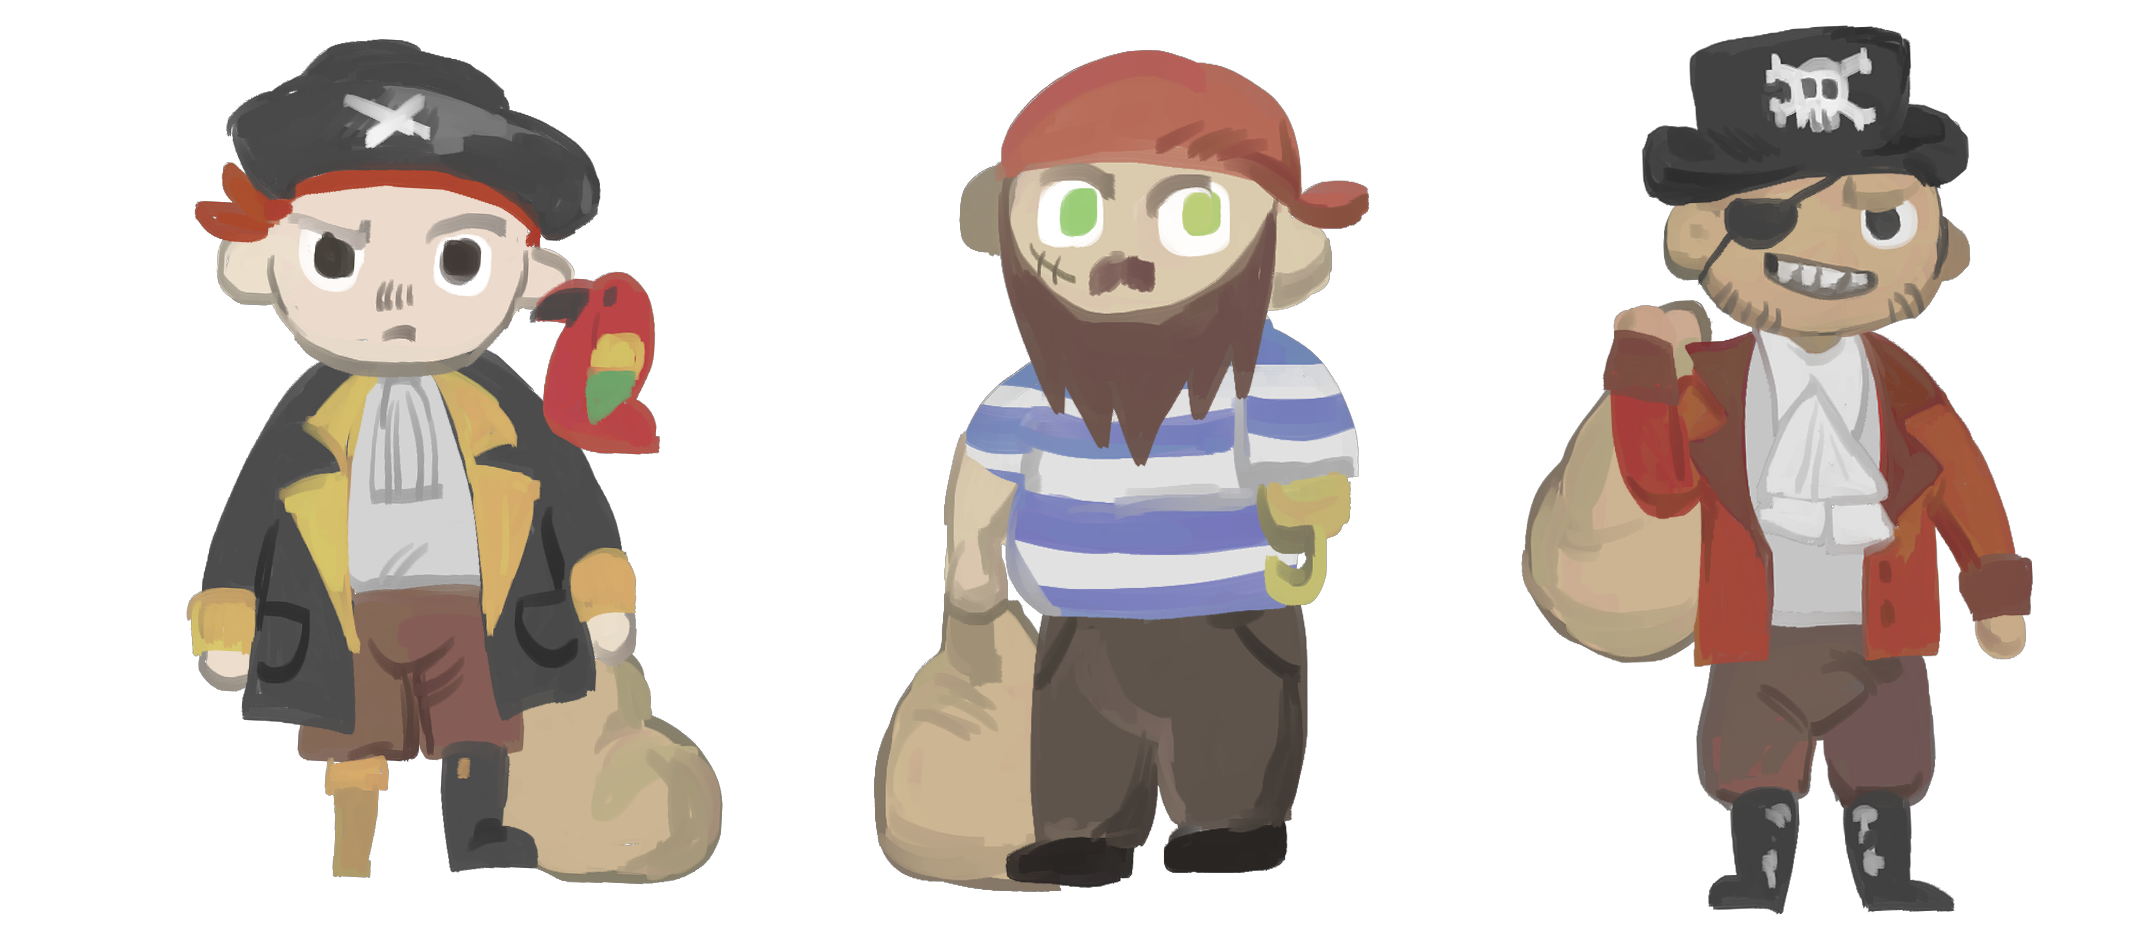
\includegraphics[width=1\linewidth]{Hinh3}
		\vspace*{-15pt}
	\end{figure}
	$\pmb{4.}$ 	Bác Tâm mua một bao tải gạo nặng $9$ kg. Bác muốn chia ra thành hai túi nhỏ hơn, một túi nặng $2$ kg, còn túi kia nặng $7$ kg. Bác chỉ có một bàn cân đĩa thăng bằng với hai quả cân, một quả nặng $50$ g, còn quả kia nặng $200$ g. Em hãy giúp bác Tâm thực hiện phép san gạo ra hai túi nhỏ như trên chỉ tối đa sau ba lần cân.
	\begin{figure}[H]
		\centering
		%		\vspace*{-5pt}
		\captionsetup{labelformat= empty, justification=centering}
		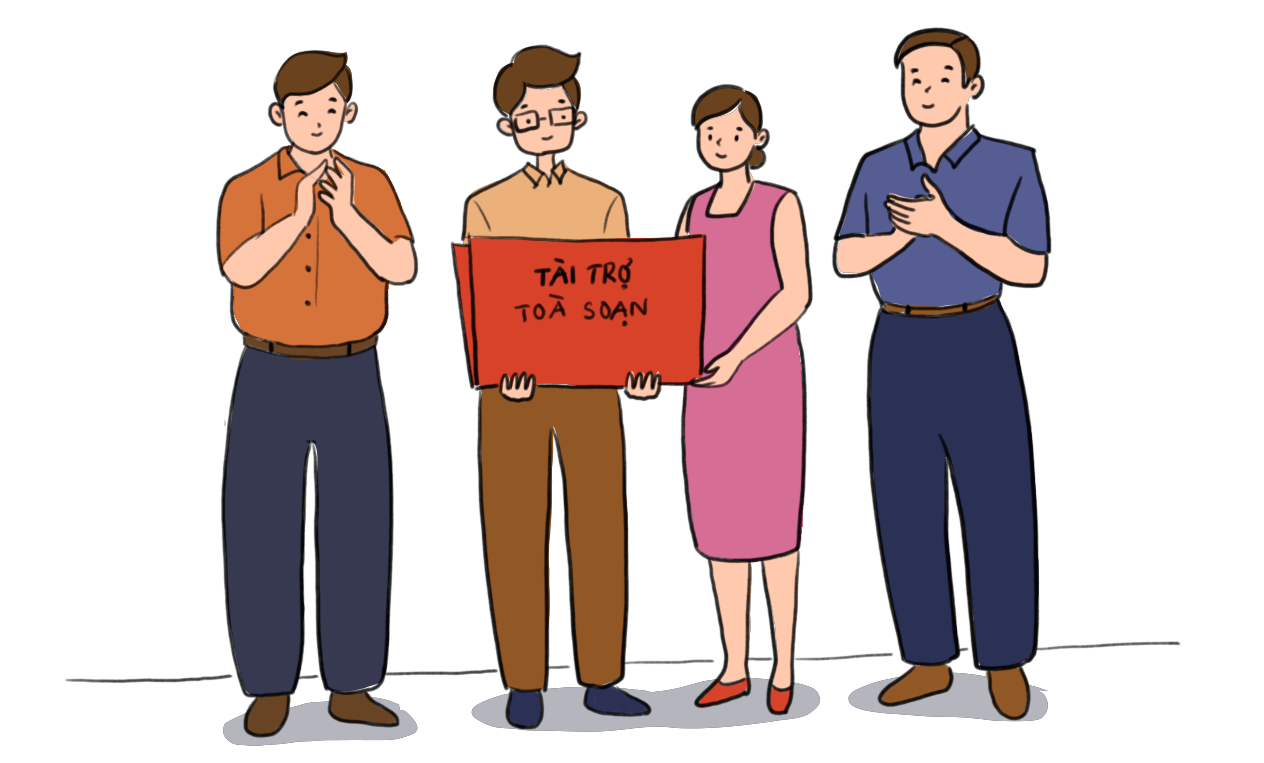
\includegraphics[width=1\linewidth]{Hinh4}
		\vspace*{-10pt}
	\end{figure}
	\vskip 0.1cm
	$\pmb{5.}$ 	Có $6$ đồng xu hình thức bên ngoài giống hệt nhau. Bốn đồng xu trong số đó là thật, mỗi đồng có khối lượng đúng $4$ g, còn hai đồng xu là giả có tổng khối lượng là $8$ g nhưng có một đồng nặng hơn một chút, còn một đồng nhẹ hơn một chút. Hỏi có thể sử dụng một bàn cân thăng bằng (không có quả cân) để sau tối đa bốn lần cân phát hiện được hai đồng xu giả được hay không?
	\begin{figure}[H]
		\centering
		\vspace*{-5pt}
		\captionsetup{labelformat= empty, justification=centering}
		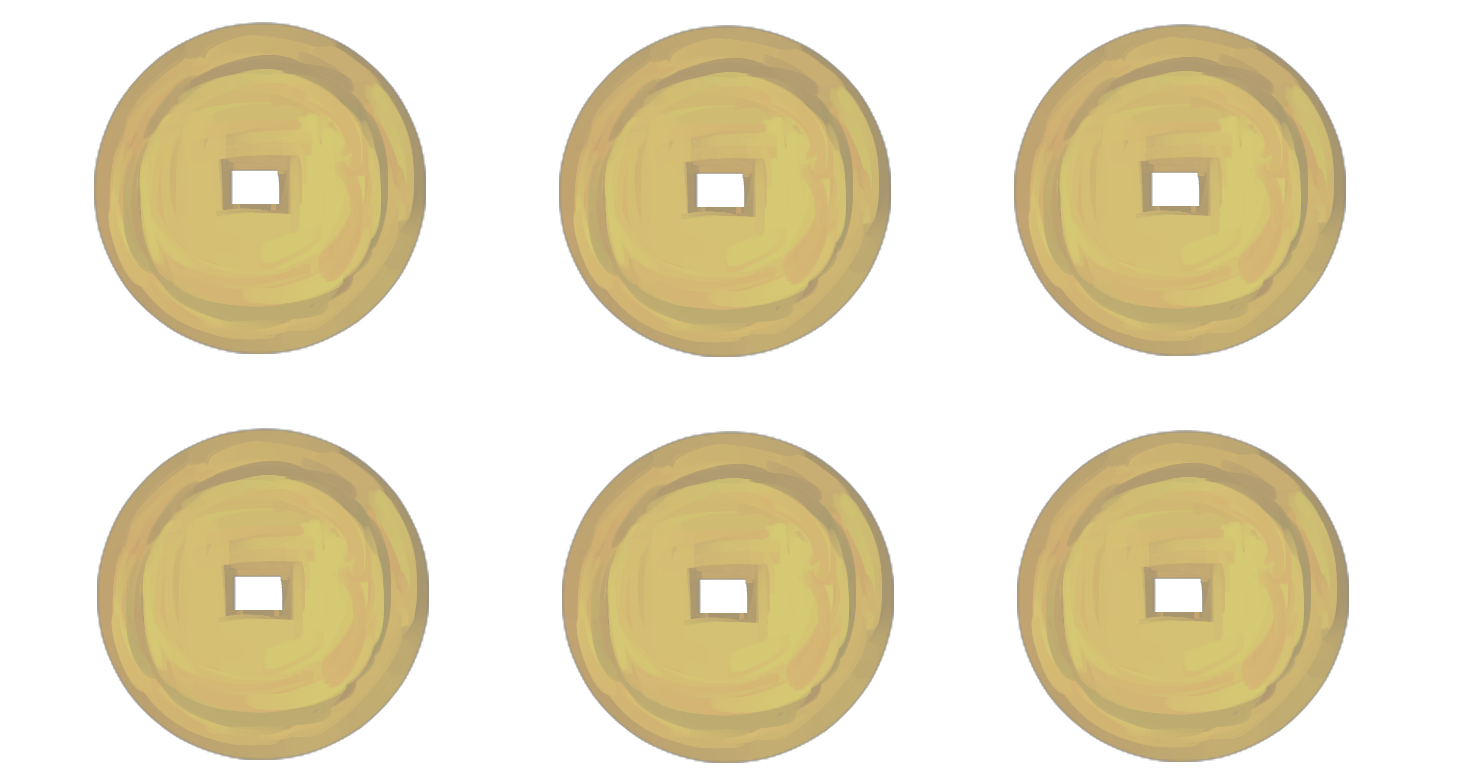
\includegraphics[width=1\linewidth]{Hinh5}
		\vspace*{-20pt}
	\end{figure}
	$\pmb{6.}$ 	Trong một giải vô địch đá bóng của trường, đội dành huy chương vàng có được tổng số điểm là $7$, đội dành huy chương bạc có tổng số điểm là $5$, còn đội dành huy chương đồng có tổng số điểm là $3$. Biết rằng trong giải đấu này các đội thi đấu theo hình thức vòng tròn $1$ lượt, mỗi đội thi đấu với một đội khác đúng một trận, và trong mỗi trận mỗi đội sẽ nhận được $2$ điểm nếu thắng, $1$ điểm nếu hoà, $0$ điểm nếu thua. Nếu hai đội có cùng tổng số điểm thì vị trí thứ tự sẽ được xác định bằng hiệu số bàn thắng và bàn thua. Hỏi 
	\vskip 0.1cm
	$a)$ Đội đứng ở vị trí thấp nhất có được tổng số điểm là bao nhiêu?
	\vskip 0.1cm
	$b)$	Có bao nhiêu đội tham gia giải vô địch.
	\begin{figure}[H]
		\centering
		\vspace*{-10pt}
		\captionsetup{labelformat= empty, justification=centering}
		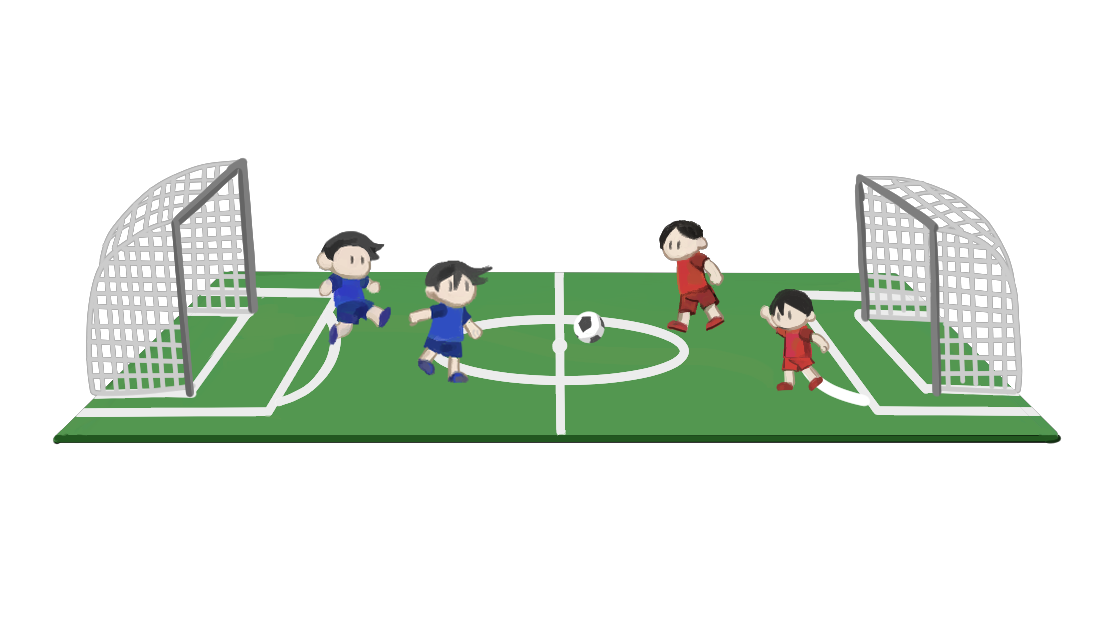
\includegraphics[width=1\linewidth]{Hinh6}
		\vspace*{-10pt}
	\end{figure}
\end{multicols}
\newpage
\begingroup
\AddToShipoutPicture*{\put(116,640){
\includegraphics[scale=1]{../tieude2.pdf}}} 
\centering
\endgroup
\vspace*{65pt}

\begin{multicols}{2}
	$\pmb{1.}$ 	Tại thành phố Hoa Hướng Dương, trong số các cậu bé tí hon có $5$ cậu ngày nào cũng ăn bánh rán ngọt, có $7$ cậu bé cứ cách một ngày lại ăn bánh rán ngọt, còn tất cả các cậu bé tí hon còn lại không bao giờ ăn bánh rán ngọt. Ngày hôm qua có $9$ cậu bé tí hon đã ăn bánh rán ngọt. Hỏi trong ngày hôm nay sẽ có bao nhiêu cậu bé tí hon ăn bánh rán ngọt?
	\begin{figure}[H]
		\centering
		\vspace*{-10pt}
		\captionsetup{labelformat= empty, justification=centering}
		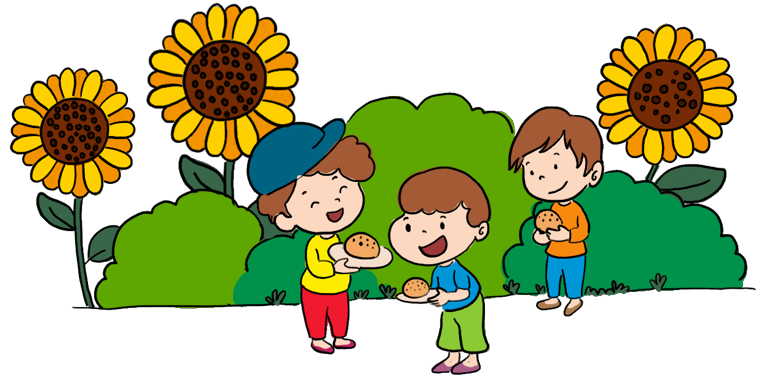
\includegraphics[width=0.9\linewidth]{Pi9_bai1}
		\vspace*{-15pt}
	\end{figure}
	\textit{Lời giải.} 	Trong số $9$ cậu bé tí hon ăn bánh rán ngọt ngày hôm qua có $5$ cậu ăn bánh rán mỗi ngày, như vậy $4$ cậu còn lại ăn bánh rán cách $1$ ngày. Do đó trong ngày hôm nay $4$ cậu này sẽ không ăn bánh rán, còn những cậu bé còn lại (có $3$ cậu) trong số các cậu ăn bánh cách $1$ ngày lại sẽ ăn bánh. Vì thế $3$ cậu này sẽ ăn bánh trong ngày hôm nay, cùng với cả $5$ cậu ăn bánh rán mỗi ngày. Ta có đáp số là: $3+5 = 8$ (cậu bé tí hon).
	\vskip 0.1cm
	$\pmb{2.}$ Một cửa hàng bán hoa tươi có ba loại hoa hồng: hồng tím, hồng vàng và hồng đỏ. Số hoa hồng tím bằng một nửa tổng số hoa hồng vàng và hồng đỏ. Số hoa hồng đỏ lại bằng một phần ba tổng số hoa hồng vàng và số hoa hồng tím. Biết rằng số hoa hồng vàng là $45$ bông. Hỏi cửa hàng có bao nhiêu hoa hồng tím và hoa hồng đỏ?
	\vskip 0.1cm
	\textit{Lời giải.} 	Số hoa hồng tím bằng một nửa tổng số hoa hồng vàng và hồng đỏ, có nghĩa là số hoa hồng tím bằng $1/3$ tổng số hoa hồng. Tương tự, số hoa hồng đỏ chiếm $1/4$ tổng số hoa hồng. Ta có thể vẽ sơ đồ đoạn thẳng, có độ dài bằng $12$ đoạn nhỏ (cho thuận tiện việc biểu diễn $1/3$ và $1/4$ tổng số). Số hoa hồng tím tương ứng $4$ đoạn nhỏ, còn số hoa hồng đỏ tương ứng $3$ đoạn. Suy ra số hoa hồng vàng tương ứng với $12 - 3 - 4 = 5$ (đoạn). Như vậy mỗi đoạn nhỏ tương ứng với $45/5 = 9$ (bông hoa). Do đó, số hoa hồng tím là $4\times 9=36$ (bông) và số hoa hồng đỏ là $3\times 9=27$ (bông).
	\begin{figure}[H]
		\centering
		\vspace*{-10pt}
		\captionsetup{labelformat= empty, justification=centering}
		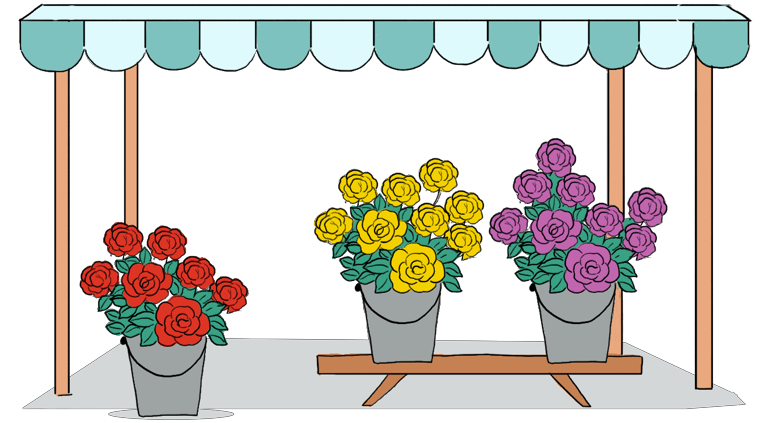
\includegraphics[width=0.8\linewidth]{Pi9_bai2}
		\vspace*{-10pt}
	\end{figure}
	$\pmb{3.}$ Thỏ Hồng đi đón $3$ cậu bạn của mình là Ngựa Đốm, Ngựa Bạch và Gấu Nâu lặn lội đến thăm nhà mình. Vừa ra tới bìa rừng, Thỏ Hồng đã thấy lờ mờ ba bạn đứng hàng ngang ở xa xa ngoài bãi cỏ, nhưng vì sương mù dày đặc, Thỏ Hồng không thể nhận ra ai với ai. Thỏ Hồng bèn kêu các bạn tự giới thiệu để biết được từng vị khách. Cậu bạn đứng ở ngoài cùng bên trái từ vị trí quan sát của Thỏ Hồng nói rằng: ``Có Gấu Nâu đứng cạnh tôi đấy". Cậu bạn đứng ở ngoài cùng bên tay phải, lại tuyên bố rằng: ``Đó là Ngựa Bạch vừa nói với cậu đấy". Cuối cùng, cậu bạn đứng ở giữa, thông báo rằng: ``Bên tay trái của tôi là Ngựa Đốm đấy". Các em hãy tìm ra bạn nào đứng ở đâu trong số $3$ người bạn của Thỏ Hồng, biết rằng Ngựa Đốm thì chuyên nói dối, Ngựa Bạch thì thỉnh thoảng nói dối, còn Gấu Nâu thì không bao giờ nói dối Thỏ Hồng.
	\vskip 0.1cm
	\textit{Lời giải.} Nếu như Gấu Nâu đứng ở ngoài cùng bên trái (từ vị trí quan sát của Thỏ Hồng), thì cậu bạn đứng giữa cũng phải là Gấu Nâu -- điều này là mâu thuẫn. Nếu như Gấu Nâu đứng ở giữa, thì bên tay phải (theo Thỏ Hồng quan sát) sẽ là Ngựa Đốm, còn bên ngoài cùng tay trái sẽ là Ngựa Bạch. Nhưng như vậy, Ngựa Đốm sẽ nói thật, ta lại suy ra mâu thuẫn.
	\begin{figure}[H]
		\centering
		\vspace*{-10pt}
		\captionsetup{labelformat= empty, justification=centering}
		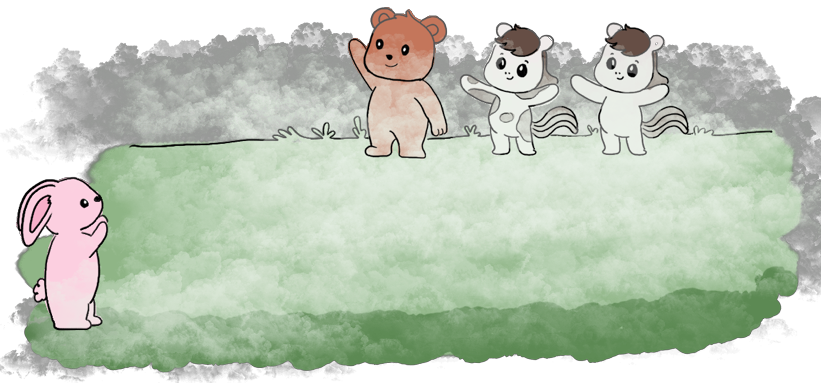
\includegraphics[width=0.85\linewidth]{Pi9_bai3}
		\vspace*{-10pt}
	\end{figure}
	Cuối cùng, chỉ khi Gấu Nâu đứng ngoài cùng bên phải ta mới không gặp mâu thuẫn. Khi đó ngoài cùng tay trái là Ngựa Bạch, ở giữa là là Ngựa Đốm -- hai cậu bạn này đều nói dối.
	\vskip 0.1cm
	\textit{Đáp số}: Từ chỗ quan sát của Thỏ Hồng, ngoài cùng tay trái là Ngựa Bạch, ở giữa là Ngựa Đốm, còn đứng ngoài cùng bên phải là Gấu Nâu.
	\vskip 0.1cm
	$\pmb{4.}$ Có $7$ quả táo, khối lượng mỗi quả có thể khác nhau để ở trên bàn. Bạn Thanh nhận thấy rằng có thể đặt $3$ quả trên một đĩa cân và $4$ quả còn lại trên đĩa cân bên kia sao cho hai bên cân thăng bằng. Bạn Thịnh lại thấy rằng có thể đặt $2$ quả táo trên một đĩa cân, và $5$ quả còn lại trên đĩa cân bên kia và hai bên cân cũng thăng bằng. Em hãy chỉ ra rằng có thể đặt trên một đĩa cân bên này $1$ quả táo và đặt trên đĩa cân bên kia $3$ quả táo trong số $7$ quả đã cho, sao cho hai bên cân cũng vẫn thăng bằng.
	\begin{figure}[H]
		\centering
		\vspace*{-10pt}
		\captionsetup{labelformat= empty, justification=centering}
		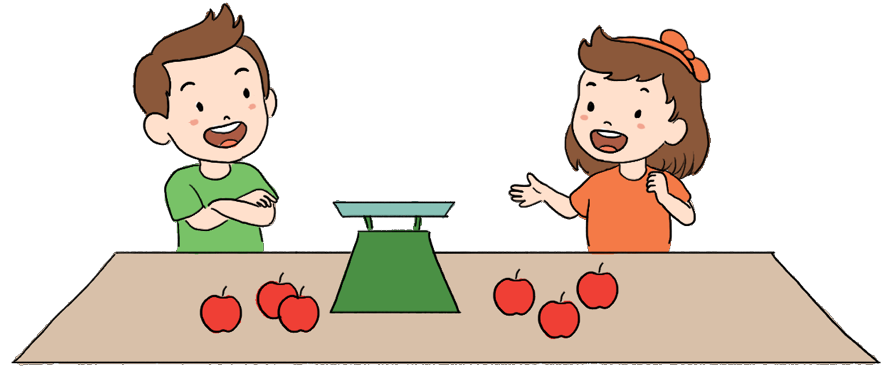
\includegraphics[width=0.85\linewidth]{Pi9_bai4}
		\vspace*{-10pt}
	\end{figure}
	\textit{Lời giải.} 	Để dễ dàng hình dung, ta có thể giả sử rằng Thanh đặt được $3$ quả táo đỏ ở đĩa cân bên trái và $4$ quả táo xanh ở đĩa cân bên phải để cân thăng bằng. Vì vậy nếu Thịnh đặt bất kỳ hai quả táo cùng màu ở một bên và $5$ quả còn lại ở đĩa bên kia thì $5$ quả này sẽ luôn nặng hơn (điều này cũng tương đương với việc có những quả táo nào đó sau lần cân thăng bằng của Thanh đã bị chuyển sang đĩa cân bên kia).
	\vskip 0.1cm
	Vì vậy để cho cân thăng bằng, Thịnh chỉ có thể đặt hai quả táo khác màu trên một đĩa cân, và $5$ quả còn lại sang đĩa bên kia. Nhưng điều này cũng tương đương với việc sau khi Thanh đã cân được thăng bằng, Thịnh đã đổi chỗ $2$ quả táo đỏ với $1$ quả táo xanh. Nếu như bỏ $3$ quả này đi, thì trên một đĩa cân có $1$ quả táo đỏ và trên đĩa bên kia có $3$ quả táo xanh, và hơn nữa cân hai bên vẫn thăng bằng.
	\vskip 0.1cm
	Các em có thể làm bài này bằng lập luận theo dạng của biểu thức đại số, lập ra hai phương trình và tìm hiệu của chúng.
	\vskip 0.1cm
	$\pmb{5.}$ Có $20$ chiếc túi nilon, mỗi túi đựng $26$ quả mận. Biết rằng tổng khối lượng của mỗi túi không vượt quá $1$ kg. Em hãy chỉ ra rằng có thể xếp số mận trên vào $26$ chiếc túi nilon, mỗi túi có đúng $20$ quả mận, sao cho tổng khối lượng của mỗi túi nhỏ hơn $1$ kg.
	\begin{figure}[H]
		\centering
		\vspace*{-10pt}
		\captionsetup{labelformat= empty, justification=centering}
		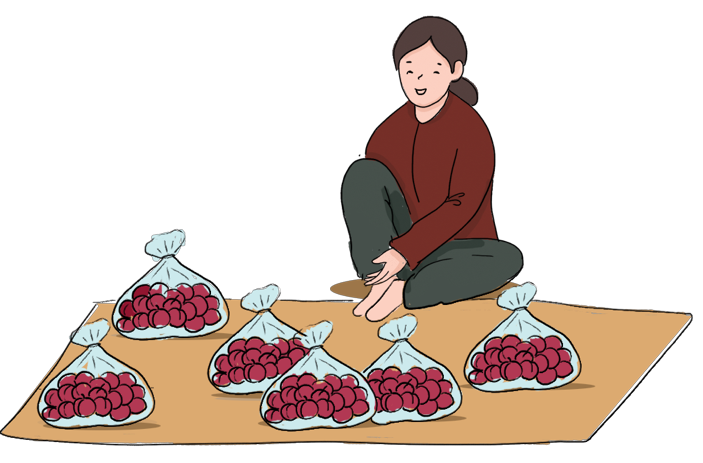
\includegraphics[width=0.85\linewidth]{Pi9_bai5}
		\vspace*{-10pt}
	\end{figure}
	\textit{Lời giải.} 	Ta nhặt ra từ mỗi túi ban đầu quả mận nhẹ nhất và xếp chúng vào chiếc túi thứ $21$. Do mỗi quả nhẹ nhất này có khối lượng không quá $\dfrac{1}{26}$ kg, nên tổng khối lượng của $20$ quả được nhặt ra này không quá $\dfrac{20}{26} <1$ (kg). Hơn nữa khối lượng của mỗi túi ban đầu giờ đều nhẹ hơn $1$ kg, và trong mỗi túi có đúng $25$ quả. Ta lại lặp lại quá trình trên: nhặt ra trong mỗi túi trong số $20$ túi ban đầu quả mận nhẹ nhất (tức là quả mận nhẹ thứ nhì, sau khi đã nhặt ra lần đầu tiên), và đưa $20$ quả này vào chiếc túi thứ $22$, khi đó tổng khối lượng mận ở chiếc túi thứ $22$ này sẽ nhỏ hơn $\dfrac{20}{25}$ (kg). Ta cứ làm như vậy, cho đến khi đạt đến chiếc túi thứ $26$ (sau $6$ lần nhặt ra).
	\vskip 0.1cm
	$\pmb{6.}$ 	Có $100$ số $1, 2, 3, \ldots, 100$ được viết ra thành hàng ngang từ trái qua phải theo thứ tự tăng dần. Bạn Long và bạn Lâm chơi một trò chơi như sau. Hai bạn lần lượt đến lượt chơi của mình sẽ đặt duy nhất một trong các dấu $+$, $-$ hoặc $\times$ vào vị trí bất kỳ xen kẽ giữa hai số trong $100$ số nói trên. Bạn đi lượt cuối cùng sẽ thắng nếu số nhận được bằng cách 
	\begin{figure}[H]
		\centering
		\vspace*{-5pt}
		\captionsetup{labelformat= empty, justification=centering}
		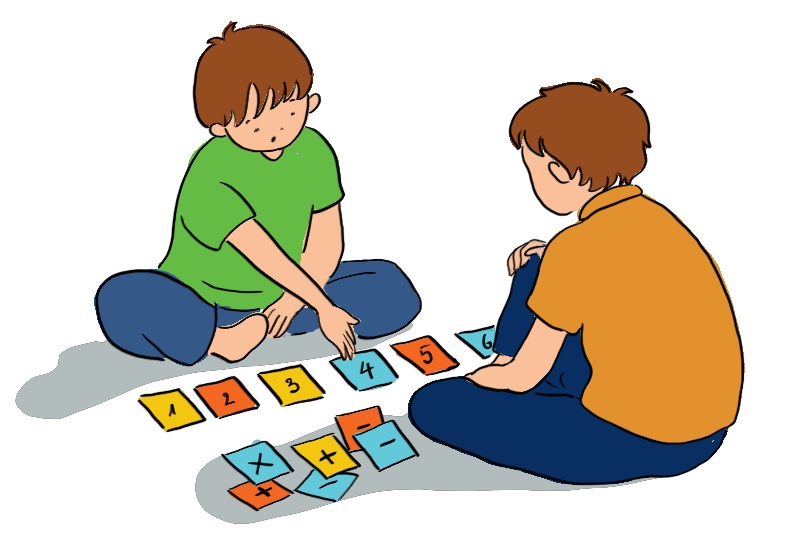
\includegraphics[width=0.7\linewidth]{Pi9_bai6}
		\vspace*{-5pt}
	\end{figure}
	 thực hiện phép tính bởi $100$ số và các phép tính đã điền giữa chúng là một số lẻ. Em hãy chỉ ra rằng nếu Long là người đi đầu tiên (và cũng sẽ là người đi cuối cùng) thì Long luôn có cách chơi để thắng.
	\vskip 0.1cm
	\textit{Lời giải.} 	Trước tiên, trong lượt đi đầu tiên, Long sẽ đặt dấu $+$ vào bên tay phải số $1$. Sau đó cứ mỗi lượt chơi của mình, Long sẽ đặt dấu $\times$ (vào bên trái hoặc bên phải) bên cạnh mỗi số lẻ trong số các số lẻ từ $3$ đến $99$. Để ý rằng Long sẽ luôn làm được như vậy, do mỗi số lẻ có hai vị trí bên cạnh có thể điền dấu. Bằng cách đặt dấu $\times$ giữa một số lẻ và một số chẵn đứng cạnh nó, Long làm cho biểu thức đứng bên phải số $1$ là một biểu thức chỉ chứa phép cộng, trừ, hoặc nhân các số chẵn với nhau, tức là biểu thức đó là một số chẵn. Vì thế kết quả nhận được ở lượt đi cuối cùng của Long sẽ luôn là một số lẻ sau khi cộng thêm $1$. 
\end{multicols}
\vspace*{-10pt}
{\color{toancuabi}\rule{1\linewidth}{0.1pt}}
\begin{multicols}{2}
	\textbf{\color{toancuabi}Đáp án}
	\vskip 0.1cm
	\textbf{\color{toancuabi}Bài $\pmb1$.} Nhận thấy Hình thứ $n$ trong dãy là một hình vuông có các đặc điểm sau:
	\vskip 0.1cm
	-- Cạnh hình vuông có kích thước là: $2\times n$;
	\vskip 0.1cm
	-- Hàng cuối có $2\times n$ dấu $\#$ và các hàng còn lại có $n$ dấu $\#$.
	\vskip 0.1cm
	Như vậy số dấu $\#$ trong Hình thứ $8$ là:
	\begin{align*}
		15\times 8 + 16 = 136. 
	\end{align*}
	\textbf{\color{toancuabi}Bài $\pmb2$.} Để hiệu nhận được là lớn nhất thì số bị trừ là số lớn nhất có $4$ chữ số và số trừ sẽ nhỏ nhất có $4$ chữ số tạo từ các số đã cho.
	\vskip 0.1cm
	Do đó số bị trừ là $3222$ và số trừ là $1001$ và ta có hiệu lớn nhất có thể là:
	\begin{align*}
		3222 - 1001 = 2221.
	\end{align*}
	\textbf{\color{toancuabi}Bài $\pmb3$.} Ta viết tên các điểm như trong hình vẽ dưới đây.
	\vskip 0.1cm
	Nhận thấy phần tô đậm có diện tích bằng tổng diện tích của các tam giác sau.
	$BKH,$ $ADE,$ $DEK,$ $CFG$ và $FGH.$
	\vskip 0.1cm
	\begin{figure}[H]
		\vspace*{5pt}
		\centering
		\captionsetup{labelformat= empty, justification=centering}
		\definecolor{zzttqq}{rgb}{0.6,0.2,0.}
		\begin{tikzpicture}[toancuabi, scale=0.9]
			\fill[color=cackithi,fill=cackithi!40] (1.,0.) -- (2.,5.) -- (3.,0.) -- cycle;
			\fill[color=zzttqq,fill=cackithi!40] (1.,0.) -- (4.,5.) -- (3.,0.) -- (0.,5.) -- cycle;
			\draw  (1.,0.)-- (2.,5.);
			\draw  (2.,5.)-- (3.,0.);
			\draw  (3.,0.)-- (1.,0.);
			\draw  (1.,0.)-- (4.,5.);
			\draw  (4.,5.)-- (3.,0.);
			\draw  (3.,0.)-- (0.,5.);
			\draw  (0.,5.)-- (1.,0.);
			
			\draw [fill=cackithi!40] (0.5,2.5) circle (2.0pt) node[anchor=north east] {$D$};
			\draw [fill=cackithi!40] (1.5,2.5) circle (2.0pt) node[above] {$E$};
			\draw [fill=cackithi!40] (2.5,2.5) circle (2.0pt) node[above] {$F$};
			\draw [fill=cackithi!40] (3.5,2.5) circle (2.0pt) node[anchor = north west] {$G$};
			\draw [fill=cackithi!40] (4.,5.) circle (2.0pt) node[above] {$C$};
			\draw [fill=cackithi!40] (0.,5.) circle (2.0pt) node[above] {$A$};
			\draw [fill=cackithi!40] (2.,5.) circle (2.0pt) node[above] {$B$};
			\draw [fill=cackithi!40] (1.,0.) circle (2.0pt) node[anchor=north east] {$K$};
			\draw [fill=cackithi!40] (3.,0.) circle (2.0pt) node[anchor = north west] {$H$};
			
			\draw[dashed]  (-1.,5.)-- (5.,5.);
			\draw[dashed]  (-1.,2.5)-- (5.,2.5);
			\draw[dashed]  (-1.,0.)-- (5.,0.);
			\draw[-stealth]  (4.5,5.)-- (4.5,2.5);
			\draw[-stealth]  (4.5,2.5)-- (4.5,0.);
			\draw[-stealth]  (1,-0.4)-- (3.,-0.4);
			
			\draw[-stealth]  (4.5,2.5) -- (4.5,5.);
			\draw[-stealth]  (4.5,0.) -- (4.5,2.5);
			\draw[-stealth]  (3.,-0.4) -- (1,-0.4);
			\draw[color=black] (4.21498164902576,3.87946061896495) node {$5$};
			\draw[color=black] (4.143071467449243,1.3626042637868525) node {$5$};
			\draw[color=black] (2.039698656336115,-0.709930933849792) node {$4$};
		\end{tikzpicture}
		\vspace*{-10pt}
	\end{figure}
	Tam giác $BKH$ có đáy $KH = 4$ và chiều cao bằng $10$, do đó có diện tích là: \begin{align*}
		\dfrac{1}{2} \times 4 \times 10 = 20.
	\end{align*}
	Các tam giác $ADE$, $DEK$, $CFG$ và $FGH$ có các đáy $DE=EF=FG = 2$ và chiều cao bằng $5$, do đó có cùng diện tích là: 
	\begin{align*}
		\dfrac{1}{2} \times 2\times 5 = 5.
	\end{align*}
	Vậy diện tích của phần tô đậm là:
	\begin{align*}
		20 + 4\times 5 = 40 \text{ (đơn vị diện tích)}
	\end{align*}
	\textbf{\color{toancuabi}Bài $\pmb4$.} Do tích của mỗi hàng và mỗi cột đều bằng nhau nên tích các số của cột thứ $2$ và hàng thứ $4$ bằng nhau. Vì cột $2$ và hàng $4$ chung nhau một ô nên tích của $3$ số còn lại bằng nhau. Từ đó, ta có
	\begin{align*}
		32\times 4\times 1 = 32\times * \times 16.
	\end{align*}
	Giải ra ta được số ở ô có dấu $*$ là $\dfrac{1}{4}$.
	\vskip 0.1cm
	\textbf{\color{toancuabi}Bài $\pmb5$.} Điền tên các đỉnh trong hình như sau.
	\begin{figure}[H]
		\vspace*{-5pt}
		\centering
		\captionsetup{labelformat= empty, justification=centering}
		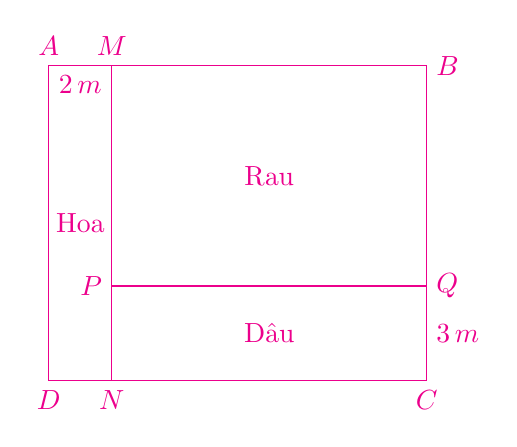
\begin{tikzpicture}[scale=0.4,toancuabi]
			\draw (0,0) rectangle (12,10);
			\draw (2,0) -- (2,10) (2,3) -- (12,3);
			\draw (0,0) node[below] {$D$};
			\draw (2,0) node[below] {$N$};
			\draw (12,0) node[below] {$C$};
			\draw (2,3) node[left] {$P$};
			\draw (12,3) node[right] {$Q$};
			\draw (12,10) node[right] {$B$};
			\draw (2,10) node[above] {$M$};
			\draw (0,10) node[above] {$A$};
			\draw (1,10) node[below] {$2\,m$};
			\draw (1,5) node {Hoa};
			\draw (7,1.5) node {Dâu};
			\draw (7,6.5) node {Rau};
			\draw (12,1.5) node[right] {$3\,m$};
		\end{tikzpicture}
		\vspace*{-10pt}
	\end{figure}
	Phần trồng hoa là hình chữ nhật $AMND$ có diện tích là $20\,m^2$. Hình chữ nhật AMND có cạnh $AM=2\,m$ nên cạnh còn lại $AD=10\,m$.
	\vskip 0.1cm
	Khu vườn là hình chữ nhật $ABCD$ có diện tích $120\, m^2$. Hình chữ nhật $ABCD$ có cạnh $AD=10\,m$ nên cạnh $DC = 12\,m$.
	\vskip 0.1cm
	Ta có
	$DC = 12 = DN + NC = 2 + NC$. Do đó $NC=10$.
	\vskip 0.1cm
	Từ đó, phần trồng dâu là hình chữ nhật $PQCN$ có hai cạnh $NC=10$ và $QC=3$. Do đó diện tích của phần trồng dâu là: $30\,m^2$.
	\vskip 0.1cm
	Vậy diện tích của phần trồng rau là: $120 - 20 - 30 = 70\,m^2$. 
	\vskip 0.1cm
	\textbf{\color{toancuabi}Bài $\pmb6$.}
	Mỗi bạn được chia $30: 3=10$ chiếc kẹo.
	\vskip 0.1cm
	Do Bình ăn một số kẹo bằng với số kẹo mà An còn nên tổng số kẹo mà An và Bình ăn là $10$ chiếc. Vì thế tổng số kẹo mà An, Bình và Chi ăn là $10+10=20$ chiếc. Do vậy, còn lại $30-20=10$ chiếc kẹo.
	\vskip 0.1cm
	\textbf{\color{toancuabi}Bài $\pmb7$.} Gọi số cây quất là $n$. Khi đó tổng tiền bán được của lần bán đầu khi cây cuối có giá $230$ nghìn là $245\times n$ và tổng tiền thu được khi bán cây cuối với giá $158$ nghìn là $242\times n$. Ta thấy chênh lệch giữa giá bán cây cuối ở $2$ lần bằng $3\times n$. Do số tiền chênh lệch giữa hai lần bán là: 
	\begin{align*}
		230-158=72 \text{ nghìn}
	\end{align*}
	nên bác nông dân đã bán được 
	\begin{align*}
		72:3 = 24 \text{ cây quất.}
	\end{align*}
	\textbf{\color{toancuabi}Bài $\pmb8$.} Ta thấy
	Cột $1$ có $2$ cách xếp bi;
	\vskip 0.1cm
	Cột $3$ có $2$ cách xếp bi;
	\vskip 0.1cm
	Cột $5$ có $1$ cách xếp  bi;
	\vskip 0.1cm
	Cột $2$ có $1$ cách xếp  bi;
	\vskip 0.1cm
	Cột $4$ có $1$ cách xếp  bi.
	\vskip 0.1cm
	Do đó, số cách xếp bi là: $2\times 2\times 1\times 1\times 1 = 4$ (cách)
	\vskip 0.1cm
	\textbf{\color{toancuabi}Bài $\pmb9$.} Gọi hai số còn khuyết ở hàng cuối là $a$ và $b$. Do mỗi ô ở hàng trên bằng tổng hai ô ngay bên dưới nên ta điền được các số như sau.
	\begin{figure}[H]
		\vspace*{-5pt}
		\centering
		\captionsetup{labelformat= empty, justification=centering}
		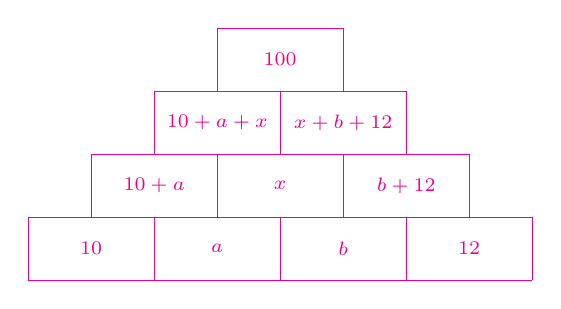
\begin{tikzpicture}[xscale=2, toancuabi,scale=0.8, node font=\scriptsize]
			\draw (0,0) grid (4,1);
			\draw (1,2) grid (3,3);
			\draw (0.5,1) rectangle (3.5,2);
			\draw (1.5,3) rectangle (2.5,4);
			\draw (1.5,1) --(1.5,2) (2.5,1) --(2.5,2);
			\draw (0.5,0.5) node {$10$};
			\draw (1.5,0.5) node {$a$};
			\draw (2.5,0.5) node {$b$};
			\draw (3.5,0.5) node {$12$};
			\draw (1,1.5) node {$10 + a $};
			\draw (2,1.5) node {$x$};
			\draw (3,1.5) node {$b+ 12$};
			\draw (1.5,2.5) node {$10 + a + x$};
			\draw (2.5,2.5) node {$x + b + 12$};
			\draw (2,3.5) node {$100$};
		\end{tikzpicture}
		\vspace*{-10pt}
	\end{figure}
	Vậy $100 = a + 10 + x + b + 12 + x = a + b + 2×x + 22$.
	\vskip 0.1cm
	Do $x = a + b$ nên $100 = 3\times x + 22$.
	\vskip 0.1cm
	Giải ra ta được $x = 26$.
	\vskip 0.1cm
	\textbf{\color{toancuabi}Bài $\pmb{10}$.} Mã PIN của bạn Kiên có dạng: $1ab3$, với $a$, $b$ là hai chữ số khác nhau và khác hai chữ số $1$, $3$.
	\vskip 0.1cm
	Ta thấy có $8$ cách chọn chữ số $a$ và $7$ cách chọn chữ số $b$.
	\vskip 0.1cm
	Do đó có $8\times 7 = 56$ cách chọn $2$ chữ số $a$ và $b$ hay có $56$ số khác nhau cho mã PIN của bạn Kiên.
\end{multicols}
\newpage
\graphicspath{{../toancuabi/toantienganh/}}
\begingroup
\thispagestyle{toancuabinone}
\blfootnote{$^1$\color{toancuabi}Ottawa, Canada.}
\AddToShipoutPicture*{\put(60,733){
\includegraphics[width=17.2cm]{../mathc.pdf}}}
%\AddToShipoutPicture*{\put(-2,733){
\includegraphics[width=17.2cm]{../mathl.pdf}}} 
\AddToShipoutPicture*{\put(106,650){
\includegraphics[scale=1]{../tieudeb.pdf}}} 
\centering
\endgroup
\vspace*{60pt}

\begin{multicols}{2}
	\setlength{\abovedisplayskip}{6pt}
	\setlength{\belowdisplayskip}{6pt}
	In this article, we will investigate a number of ways to \textit{prove area equality without writing lengthy proofs.}
	While it sounds simple, easy, and exciting, it is important that you need to improve your creative thinking in order to 
	first understand the examples, and then use them as tools, guidelines, or ideas to solve the problems.
	\vskip 0.2cm
	\PIbox{
		\textbf{\color{toancuabi}Example $\pmb1$.}
		Let $E$ be a point inside the parallelogram $ABCD$. Prove that
		\begin{align*}
			[AEB] + [CED] = \half [ABCD].
		\end{align*}
		Here, we denote the area of a region $[\pazocal{R}]$ by $\pazocal{R}$.}
	\begin{figure}[H]
		\vspace*{-10pt}
		\centering
		\captionsetup{labelformat= empty, justification=centering}
		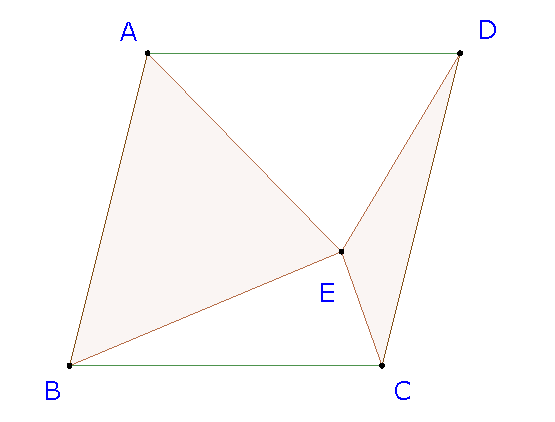
\includegraphics[width= 1\linewidth]{23-24-s3-i-p1.pdf}
		%		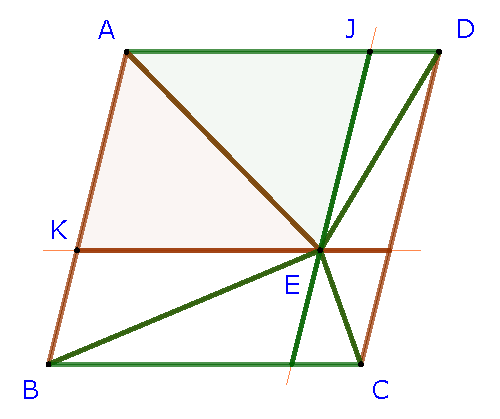
\includegraphics[width= 1\linewidth]{23-24-s3-i-p1-s.pdf}
		\vspace*{-25pt} 
	\end{figure}
	\textit{Solution.}
	Draw lines through $E,$ parallel with sides of $ABCD,$ dividing the parallelogram into four smaller parallelograms.
	Any of the smaller parallelogram, say $AKEJ$, consists of a brown triangle from the shaded triangle and a green triangle with the same area.
	Thus, the area of the shaded triangles is the sum of the area of all smaller brown triangles, which is half of the sum of the area of all smaller parallelograms,
	or half of the $ABCD$ parallelogram.
	\begin{figure}[H]
		%		\vspace*{-10pt}
		\centering
		\captionsetup{labelformat= empty, justification=centering}
		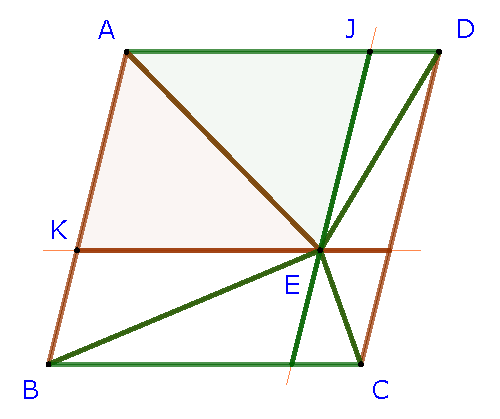
\includegraphics[width= 0.95\linewidth]{23-24-s3-i-p1-s.pdf}
		\vspace*{-10pt} 
	\end{figure}
	\textbf{\color{toancuabi}Remark.} Here's how we use the techniques:
	\vskip 0.1cm
	$1.$ First, divide the given figure into smaller figures.
	\vskip 0.1cm
	$2$. Deal with each of them, if they have the same shape, then work in the same way.
	\vskip 0.1cm
	$3.$ Use all partial results to arrive at the overall result.
	\vskip 0.2cm
	\PIbox{\textbf{\color{toancuabi}Example $\pmb2$.}
		Let $E$ and $F$ be the midpoints of $BC$ and $DA$ in the convex quadrilateral $ABCD$. Prove that
		\begin{align*}
			[AECF] = \half [ABCD].
	\end{align*}}
	\begin{figure}[H]
		\vspace*{-10pt}
		\centering
		\captionsetup{labelformat= empty, justification=centering}
		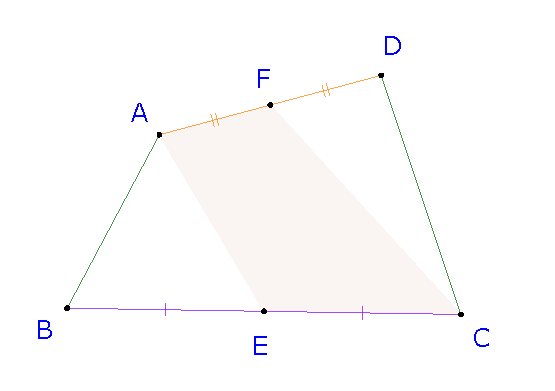
\includegraphics[width= 1\linewidth]{23-24-s3-i-p2.pdf}
		%		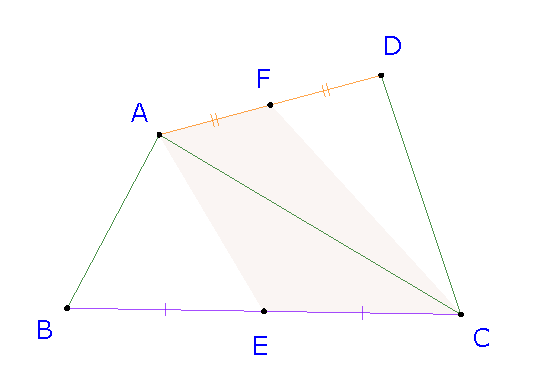
\includegraphics[width= 0.9\linewidth]{23-24-s3-i-p2-s.pdf}
		\vspace*{-20pt}
	\end{figure}
	\textit{Solution.}
	Connect $AC.$ Since $E$ is the midpoint of $BC$, the triangles $ABE$ and $AEC$ have the same area. The triangles $ABE$ and $AEC$ have the same area.
	Similarly triangles $CDF$ and $CFA$ have the same area. Thus the area of $AECF$ is half of $ABCD.$
	\begin{figure}[H]
		\vspace*{-5pt}
		\centering
		\captionsetup{labelformat= empty, justification=centering}
		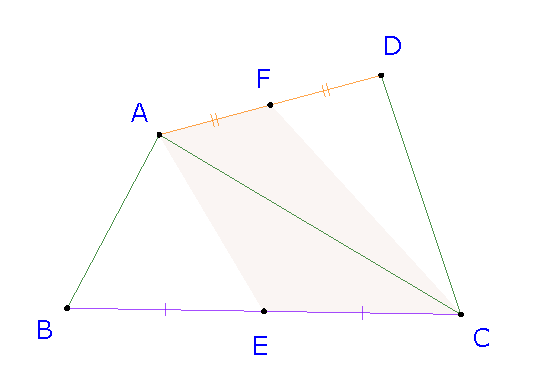
\includegraphics[width= 1\linewidth]{23-24-s3-i-p2-s.pdf}
		\vspace*{-10pt}
	\end{figure}
	\PIbox{\textbf{\color{toancuabi}Example $\pmb3$.}
		Let $I$ be an arbitrary point on the diagonal $BD$ in the parallelogram $ABCD$. Lines through $I$ parallel with the sides of $ABCD$ intersect $AB,$ $BC,$ $CD,$ and $DA$ at $E, F, G,$ and $H,$ respectively. Prove that
		\begin{align*}
			[AEIH] = [FCGI].
	\end{align*}}
	\begin{figure}[H]
		\vspace*{-5pt}
		\centering
		\captionsetup{labelformat= empty, justification=centering}
		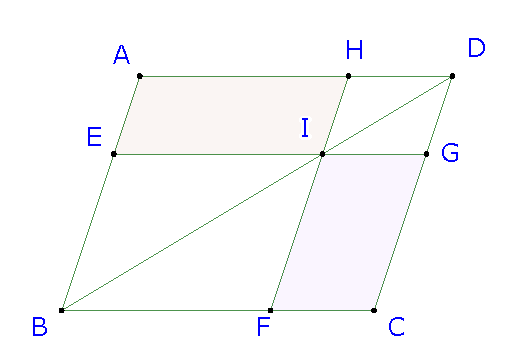
\includegraphics[width= 1\linewidth]{23-24-s3-i-p3.pdf}
		\vspace*{-10pt}
	\end{figure}
	\textit{Solution.}
	First, since $BD$ is the diagonal in parallelogram $ABCD,$ $[ABD] = [BCD].$
	Now, $BEIF$ is also a parallelogram, thus $[BEI] = [BFI],$ similarly $[HID] = [IGD].$
	Therefore 
	\begin{align*}
		[AEIH] &= [ABD] - [BEI] - [HID] \\
		&= [BCD] - [BFI] - [IGD] \\
		&= [FCGI].
	\end{align*}
	\begin{figure}[H]
		\vspace*{-5pt}
		\centering
		\captionsetup{labelformat= empty, justification=centering}
		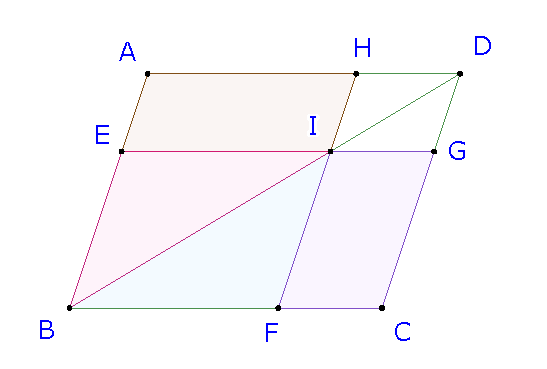
\includegraphics[width= 1\linewidth]{23-24-s3-i-p3-s.pdf}
		\vspace*{-10pt}
	\end{figure}
	\PIbox{\textbf{\color{toancuabi}Example $\pmb4$.} 
		Let $G$ and $H$ be the midpoints of $BC$ and $CD$ in the regular hexagon $ABCDEF$. The lines $EG$ and $FG$ intersect at $I$.  Prove that
		\begin{align*}
			[GCHI] = [EFI].
	\end{align*}}
	\begin{figure}[H]
		\vspace*{-5pt}
		\centering
		\captionsetup{labelformat= empty, justification=centering}
		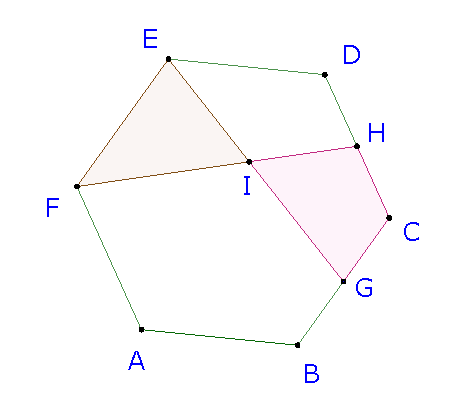
\includegraphics[width= 1\linewidth]{23-24-s3-i-p4.pdf}
		\vspace*{-10pt}
	\end{figure}
	\textit{Solution.}
	It is easy to see that the quadrilaterals $GCDE$ and $HDEF$ are congruent, thus have the same area, or $[GCDE] = [HDEF].$
	Taking $HDEI$ away, we have $[GCHI] = [EFI].$ 
	\vskip 0.2cm
	\PIbox{\textbf{\color{toancuabi}Example $\pmb5$.}
		Let $E, F, G$ and $H$ are the midpoints of the sides $AB, BC, CD$ and $DA$ in the convex quadrilateral $ABCD$.
		Prove that
		\begin{align*}
			[EFGH] = \half [ABCD].
	\end{align*}}
	\begin{figure}[H]
		\vspace*{-5pt}
		\centering
		\captionsetup{labelformat= empty, justification=centering}
		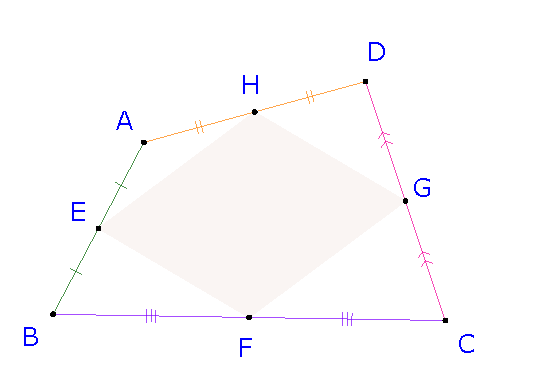
\includegraphics[width= 1\linewidth]{23-24-s3-i-p5.pdf}
		\vspace*{-10pt}
	\end{figure}
	\textit{Solution.}
	Note that $EH$ is the midsegment (the segment joining two midpoints) in the triangle $ABD$, therefore $[AEH] = \frac{1}{4}[ABD].$
	Similarly $[BEF] = \frac{1}{4}[ABC],$ $[CFG] = \frac{1}{4}[BCD],$ and $[GDH] = \frac{1}{4}[CDA],$ therefore:
	\begin{align*}
		&[AEH] + [BEF] + [CFG] + [GDH] \\
		&= \half [ABCD]\\
		\Rightarrow  &[EFGH] = \half [ABCD].
	\end{align*} 
\end{multicols}
\vskip 0.1cm
\PIbox{
	\centerline{\textbf{\color{toancuabi}Vocabulary}}
	\vskip 0.2cm
	\begin{multicols}{2}
		{\color{toancuabi}Arbitrary:} (tt) bất kỳ, tùy ý.
		\vskip 0.1cm	
		{\color{toancuabi}Area:} (dt) diện tích.
		\vskip 0.1cm
		{\color{toancuabi}Congruent:} (tt) bằng nhau.
		\vskip 0.1cm
		{\color{toancuabi}Connect:} (đt) nối.
		\vskip 0.1cm
		{\color{toancuabi}Convex:} (tt) lồi.
		\vskip 0.1cm
		{\color{toancuabi}Diagonal:} (dt) đường chéo
		\vskip 0.1cm
		{\color{toancuabi}Divide:} (đt) chia.
		\vskip 0.1cm
		{\color{toancuabi}Draw:} (đt) kẻ, vẽ.
		\vskip 0.1cm
		{\color{toancuabi}Figure:} (dt) hình.
		\vskip 0.1cm
		{\color{toancuabi}Hexagon:} (dt) lục giác,
		\vskip 0.1cm
		{\color{toancuabi}regular hexagon:} lục giác đều.
		\vskip 0.1cm
		{\color{toancuabi}Intersect:} (đt) cắt nhau, giao nhau.
		\vskip 0.1cm
		{\color{toancuabi}Line:} (dt) đường thẳng.
		\vskip 0.1cm
		{\color{toancuabi}Midpoint:} (dt) trung điểm. 
		\vskip 0.1cm
		{\color{toancuabi}Midsegment:} (dt) đường trung bình.
		\vskip 0.1cm
		{\color{toancuabi}Point:} (dt)  điểm.
		\vskip 0.1cm
		{\color{toancuabi}Parallelogram:} (dt) hình bình hành.
		\vskip 0.1cm
		{\color{toancuabi}Quadrilateral:} (dt)  tứ giác.
		\vskip 0.1cm
		{\color{toancuabi}Segment:} (dt) đoạn thẳng.
		\vskip 0.1cm
		{\color{toancuabi}Shape:} (dt) hình dáng.
		\vskip 0.1cm
		{\color{toancuabi}Side:} (dt) cạnh.
		\vskip 0.1cm
		{\color{toancuabi}Triangle:} (dt)  tam giác.
		\vskip 0.1cm
		{\color{toancuabi}Technique:} (dt) kỹ thuật.
	\end{multicols}
}

	\newpage 
%
%	\thispagestyle{empty}
%	\begingroup 
%	\AddToShipoutPicture*{\put(0,0){\includegraphics[width=19.5cm]{MV.pdf}}}
%	\centering
%	\vspace*{0cm}
%	\endgroup
%	\newpage	
%	\pagestyle{empty}
%
%	\setcounter{figure}{0}
%	\thispagestyle{hoccungpinone}
\pagestyle{hoccungpi}
\everymath{\color{hoccungpi}}
\graphicspath{{../hoccungpi/pic/}}
\blfootnote{$^{1}$\color{hoccungpi}Lớp $12$ Toán $1$, Trường THPT Amsterdam, Hà Nội.}
\blfootnote{$^{2}$\color{hoccungpi}Khoa Toán -- Tin, Đại học Sư Phạm Hà Nội.}
\begingroup
\AddToShipoutPicture*{\put(0,616){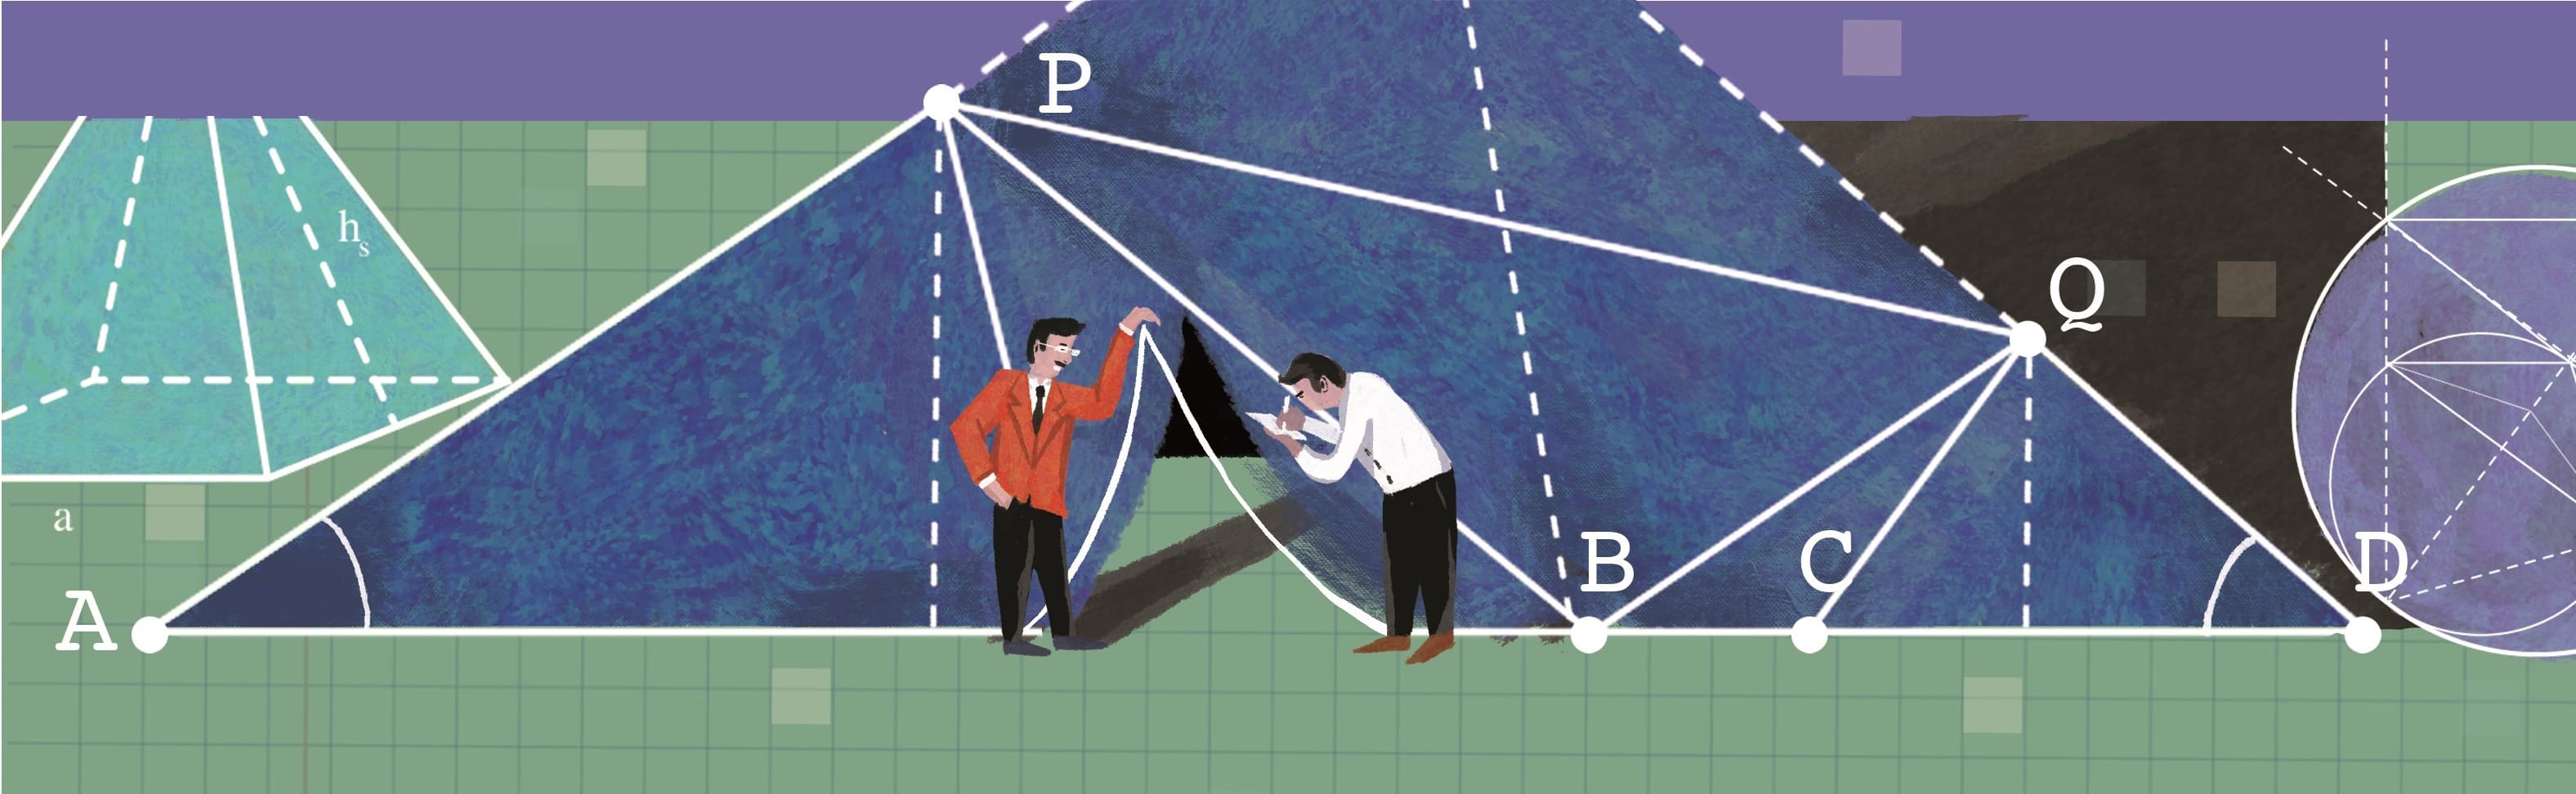
\includegraphics[width=19.3cm]{../bannerhoccungpi}}}
\AddToShipoutPicture*{\put(80,550){
\includegraphics[scale=1]{../tieude1.pdf}}}
\centering
\endgroup

\vspace*{160pt}

\begin{multicols}{2}
$\pmb{1.}$ \textbf{\color{hoccungpi}Giới thiệu}
\vskip 0.1cm
Định lý Fermat lớn nói về sự không tồn tại bộ ba số nguyên $a,b,c$ khác $0$ sao cho $a^n+b^n=c^n$ với $n\ge 3$ là số nguyên dương, đã được Andrew Wiles [$5$] chứng minh vào năm $1995$, nhưng ít ai biết rằng có một định lý ``Fermat" tương tự cho đa thức đã được chứng minh trước đó hàng chục năm trước, tức không tồn tại ba đa thức $f(x),g(x),h(x)$ với hệ số thực, ít nhất một đa thức khác đa thức hằng, đôi một không có nghiệm chung sao cho $f(x)^n+g(x)^n=h(x)^n,$ với $ n\ge 3$ là một số nguyên dương cho trước.
\vskip 0.1cm
Định lý Fermat cho đa thức là hệ quả của Định lý Mason -- Stothers, đầu tiên được Stothers [$4$] chứng minh vào năm $1981$, và Mason [$3$] độc lập phát hiện ra sau đó ít lâu. Các chứng minh đó nhìn chung là phức tạp, không sơ cấp. Năm $2000$, Snyder [$2$] đã đưa ra một chứng minh mới, chỉ với các kiến thức toán phổ thông cho định lý này. Trong bài viết này, chúng tôi giới thiệu chứng minh của Snyder và sau đó áp dụng Định lý Mason--Stothers để chứng minh Định lý Fermat cho đa thức và một số kết quả liên quan khác.
\vskip 0.1cm 
$\pmb{2. }$ \textbf{\color{hoccungpi}Định lý Mason -- Stothers}
\vskip 0.1cm
	\textbf{\color{hoccungpi}Định lý} $\pmb{1}$ (Mason -- Stothers)\textbf{\color{hoccungpi}.} 
\textit{	Cho $a(x),$ $b(x)$ và $c(x)$ là các đa thức khác đa thức hằng, với hệ số thực, đôi một không có nghiệm phức chung và thỏa mãn: $a(x) + b(x) = c(x)$. Khi đó
	\begin{align*}
		\deg(c) \le n_0{(abc)} - 1,
	\end{align*}
	trong đó ta ký hiệu $n_0(f)$ là số nghiệm phức phân biệt của đa thức $f(x)$ và $\deg(f)$ là bậc của đa thức $f(x).$}
	\vskip 0.1cm
	Để chứng minh Định lý này, ta cần Bổ đề sau:
	\vskip 0.1cm
	\textbf{\color{hoccungpi}Bổ đề} $\pmb{1.}$
	\textit{Cho $f(x)$ là một đa thức với hệ số thực, khác đa thức $0$.  Khi đó,
	\begin{align*}
		\deg(f) \le \deg(f,f') + n_0(f),
	\end{align*}
	trong đó ta ký hiệu $(f,f')$ là ước chung lớn nhất của hai đa thức $f(x)$ và $f'(x)$ ($f'(x)$ là đa thức đạo hàm của đa thức $f(x)$).} 
	\vskip 0.1cm
	\textit{Chứng minh.}
	Gọi $\alpha_1, \alpha_2, \ldots,  \alpha_m $ là các nghiệm phức phân biệt của $f(x)$ với các bội $a_1, a_2, \ldots , a_m$ tương ứng. Khi đó, ta có phân tích
	\begin{align*}
		f(x) \!=\! a(x \!-\! \alpha_1)^{a_1}(x \!-\! \alpha_2)^{a_2}\ldots (x \!-\! \alpha_m)^{a_m},
	\end{align*}
	với $a\in \mathbb{R}$ và $a_1+a_2+\cdots+a_m=\deg f(x).$
	Ta có, theo công thức Leibniz, đạo hàm của $f(x)$ được cho bởi:
	\begin{align*}
		&f'(x) \\
		=\,\,& aa_1(x - \alpha_1)^{a_1-1}(x - \alpha_2)^{a_2} \ldots (x - \alpha_m)^{a_m}  \\
		&\!+  a(x - \alpha_1)^{a_1} [(x - \alpha_2)^{a_2}\ldots(x - \alpha_m)^{a_m}]'.
	\end{align*}
	Suy ra, với mỗi $i=1, 2, \ldots, m$, đa thức $(x-\alpha_i)^{a_i-1}$ cùng là ước của $f(x)$ và $f'(x)$.
	Do đó 
	\begin{align*}
		&(x - \alpha_1)^{a_1 - 1}(x - \alpha_2)^{a_2 - 1} \ldots \\
		&(x - \alpha_m)^{a_m - 1} \mid (f,f').
	\end{align*} 
	Vì $f(x)$ là đa thức khác đa thức hằng nên $f'(x)$ khác đa thức $0$ và do đó $(f, f')$ cũng khác đa thức $0$. Suy ra
	\begin{align*}
		&\deg((x - \alpha_1)^{a_1 - 1}(x - \alpha_2)^{a_2 - 1}\ldots \\
		&(x - \alpha_m)^{a_m - 1}) \leq \deg(f,f'),
	\end{align*} 
	hay 
	\begin{align*}
		&(a_1-1)+(a_2-1)+\cdots+(a_m-1)\\
		\leq \,&\deg (f,f').
	\end{align*}
	Suy ra
	\begin{align*}
		\deg(f) - n_0(f) \leq \deg(f,f').
	\end{align*}
	Vậy bổ đề được chứng minh
	\vskip 0.1cm
	\textit{Chứng minh Định lý} $1.$
	Từ giả thiết 
	\begin{align*}
		a + b = c, \tag{$1$} 
	\end{align*}
	bằng cách lấy đạo hàm hai vế, ta được
	\begin{align*}
		a' + b' = c'. \tag{$2$}
	\end{align*}
	Nhân ($1$) với $a'$ và nhân ($2$) với $a$ và trừ vế với vế, ta được
	\begin{align*}
		a'b - ab' = a'c - ac'.
	\end{align*}
	Suy ra $(a,a'), (b,b')$ và $(c,c')$ đều là ước của $a'b - ab'$.
	\vskip 0.1cm
	Do các đa thức $a,b,c$ đôi một không có nghiệm phức chung nên các đa thức $(a,a'), (b,b')$ và $(c,c')$ cũng đôi một không có nghiệm phức chung. Suy ra
	\begin{align*}
		(a,a')(b,b')(c,c') \mid a'b - ab'.
	\end{align*}
	Hơn nữa, ta có $a'b - ab'\ne 0$. Thật vậy, nếu $ a'b - ab'= 0$ thì $\left(\dfrac{a}{b}\right)'=0$ hay $\dfrac{a}{b}$ là hằng số. Do đó $a$ và $b$ có nghiệm chung (mâu thuẫn với giả thiết).
	Vì vậy, 
	\begin{align*}
		\deg ((a,a')(b,b')(c,c'))\leq \deg(a'b - ab').
	\end{align*} 
	Mặt khác, hiển nhiên ta có 
	\begin{align*}
		\deg(a'b-ab')&\leq \max\{\deg(a'b),\deg(ab')\}\\
			&=\deg(a)+\deg(b)-1.
	\end{align*}
	Vì thế,
	\begin{align*}
		&\deg(a,a') + \deg(b,b') + \deg(c,c') \\
		\leq \,&\deg(a) + \deg(b) - 1.
	\end{align*}
	Chuyển vế bất đẳng thức này và cộng với $\deg (c)$ vào hai vế, ta được 
	\begin{align*}
		\deg(c) \leq& \deg(a) - \deg(a,a') + \deg(b) \\
		&\!\!\!-\! \deg(b,b') \!+\! \deg(c) \!-\! \deg(c,c')\!-\!1.
	\end{align*} 
	Cuối cùng, áp dụng Bổ đề $1$, ta có:
	\begin{align*}
		&\deg(a) - \deg(a,a') \leq n_0{(a)},\\
		&\deg(b) - \deg(b,b') \leq n_0{(b),}\\
		&\deg(c) - \deg(c,c') \leq n_0{(c)},
	\end{align*}
	Từ đó suy ra 
	\begin{align*}
		\deg(c) &\le n_0{(a)} + n_0{(b)} + n_0{(c)} - 1 \\
		&= n_0{(abc)} - 1.
	\end{align*}
	$\pmb{3.}$ \textbf{\color{hoccungpi}Định lý Fermat cho đa thức}
	\vskip 0.1cm
	Áp dụng Định lý Mason -- Stothers, chúng ta có một số kết quả đáng lưu ý. Trước hết, ta có kết quả sau đây:
	\vskip 0.1cm
	\textbf{\color{hoccungpi}Định lý} $\pmb{2}$  (Davenport [$1$])\textbf{\color{hoccungpi}.} \textit{Cho $f(x),g(x)$ là các đa thức với hệ số thực, khác đa thức hằng, đôi một không có nghiệm phức chung. Đặt $h(x)=(f(x))^3-(g(x))^2$ và giả sử $h(x)$ khác là đa thức $0$. Khi đó, $\deg (f) \leq 2\deg (h)-2$.}
	\vskip 0.1cm
	\textit{Chứng minh.}
	Do $f(x)$ và $g(x)$ là các đa thức không có nghiệm chung và $h = f^3 - g^2$ nên $h, f^3$ và $g^2$ đôi một không có nghiệm chung.  Áp dụng Định lý Mason -- Stothers cho ba đa thức $ g^2, h$ và $f^3,$ ta có:
	\begin{align*}
		\deg(f^3) \leq n_0{(g^2hf^3)} - 1,
	\end{align*}
	hay 
	\begin{align*}
		3\deg (f)\leq n_0{(ghf)}-1\leq \deg(ghf) - 1.
	\end{align*}
	Mà $\deg(ghf)= \deg(g) + \deg(h) +\deg(f)$, nên 
	\begin{align*}
		&3\deg(f)\\
		\leq \, &\deg(g) + \deg(h) +\deg(f)-1. \tag{$3$}
	\end{align*}
	Chứng minh tương tự, ta có:
	\begin{align*}
		&2\deg(g) \\
		\leq \, &\deg(g) + \deg(h) +\deg(f) - 1.\tag{$4$}
	\end{align*}
	Kết hợp ($3$) và ($4$), ta được
	\begin{align*}
		&3\deg(f) + 2\deg(g) \\
		\leq \,&2(\deg(g) + \deg(h) +\deg(f) - 1)
	\end{align*}
	hay $\deg(f) \leq 2\deg(h) - 2.$ Ta có điều phải chứng minh.
	\vskip 0.1cm
	\textbf{\color{hoccungpi}Hệ quả} $\pmb{1.}$
	\textit{Không tồn tại hai đa thức với hệ số thực $f(x)$ và $g(x)$, khác đa thức hằng sao cho $f^3-g^2$ là đa thức hằng khác đa thức $0$.}
	\vskip 0.1cm
	Như đã đề cập đến trong phần đầu của bài viết, định lý Mason--Stothers có thể được sử dụng để chứng minh phiên bản đa thức của định lý Fermat lớn.
	\vskip 0.1cm
	\textbf{\color{hoccungpi}Định lý} $\pmb{3}$ (Định lý Fermat cho đa thức)\textbf{\color{hoccungpi}.} \textit{Với mọi nguyên $n\ge 3$, không tồn tại ba đa thức $f(x),g(x),h(x)$, với hệ số thực, đôi một không có nghiệm phức chung, trong đó ít nhất một đa thức khác đa thức hằng, sao cho $f^n+g^n=h^n$.}
	\vskip 0.1cm
	\textit{Chứng minh.}
	Giả sử ngược lại, $f^n+g^n=h^n$. Áp dụng định lý Mason--Stothers cho $3$ đa thức $f^n, g^n$ và $h^n$, ta có:
	\begin{align*}
		&\max\{\deg(f^n), \deg(g^n), \deg(h^n)\} \\
		\le\, &n_0{(f^ng^nh^n)} - 1 = n_0{(fgh)} - 1 \\
		\le\, &\deg(f) + \deg(g) + \deg(h) - 1.
	\end{align*}
	Để ý rằng
	\begin{align*}
		&\dfrac{n}{3}(\deg(f) + \deg(g) + \deg(h)) \\
		=    \,&\dfrac{1}{3}(\deg(f^n) + \deg(g^n) + \deg(h^n)) \\
		\le\,& \max\{\deg(f^n), \deg(g^n), \deg (h^n).
	\end{align*}
	Do đó, nếu ta đặt $d=\deg(f) + \deg(g) + \deg(h)$ thì bằng cách kết hợp với bất đẳng thức thu được ở trên, ta có:
	\begin{align*}
		\dfrac{nd}{3} \le d - 1.
	\end{align*}
	Suy ra, $3 < d(3-n).$ Do ít nhất một trong các đa thức $f, g, h$ khác hằng nên $d >0$; điều này, kết hợp với giả thiết $n\ge 3$, dẫn đến $3\le 0$, mâu thuẫn. 
	\vskip 0.1cm
	Với chứng minh tương tự, ta có thể chỉ ra được hệ quả sau đây, mà nội dung của nó là một bài toán trong tuyển tập Các kỳ thi Toán Rumani (RMC) năm $2019$.
	\vskip 0.1cm
	\textbf{\color{hoccungpi}Hệ quả} $\pmb{2.}$ \textit{Cho các số nguyên $m,n\ge 3$ và $f,g$ là các đa thức khác hằng với hệ số thực, trong đó ít nhất một đa thức có bậc lớn hơn hoặc bằng $2$. Giả sử $\deg (f^m-g^n)<\min \{m,n\}$. Khi đó $f^m=g^n$.}
	\vskip 0.1cm
	\textbf{\color{hoccungpi}Nhận xét.}
	Định lý Mason -- Stothers cũng đúng khi ta xét các đa thức với hệ số phức. Từ đó ta suy ra Định lý Davenport và Định lý Fermat cho đa thức cũng đúng với đa thức với hệ số phức.
	\vskip 0.1cm
	Để kết thúc, chúng ta trình bày một mở rộng của Định lý $3$.
	\vskip 0.1cm
	\textbf{\color{hoccungpi}Định lý} $\pmb{4.}$ \textit{Cho các số nguyên dương $m,n,p$ thỏa mãn $m\leq n\leq p$. Khi đó phương trình đa thức $f(x)^m+g(x)^n=h(x)^p$ có nghiệm $f,g,h$ là các đa thức với hệ số phức, đôi một không có nghiệm chung, ít nhất một trong ba đa thức khác đa thức hằng nếu và chỉ nếu $(m,n,p)$ có một trong dạng sau: $(1,a,b), a,b\ge 1$; $(2,2,a), a\ge 2$; $(2,3,3); (2,3,4); (2,3,5)$.}
	\vskip 0.1cm
	\textit{Chứng minh.}
	Trước hết, dễ thấy rằng nếu trong $m, n, p$ có một số bằng $1$ thì phương trình rõ ràng có nghiệm, chẳng hạn nếu $m=1$, với $g(x),h(x)$ là hai đa thức khác đa thức hằng tùy ý, không có nghiệm chung thì bằng cách đặt $f(x)=h(x)^p-g(x)^m$, ta có $f(x), g(x), h(x)$ thỏa mãn phương trình.
	\vskip 0.1cm
	Vì vậy, ta chỉ cần xét trường hợp $ 2 \le m \le n \le p$. Gọi $a, b, c$ lần lượt là bậc của các đa thức $f, g$ và $h$. Khi đó, theo Định lý Mason -- Stothers, ta có
	\begin{align*}
		ma \le a + b + c - 1, \tag{$5$}\\
		nb \le a + b + c - 1, \tag{$6$}\\
		pc \le a + b + c - 1. \tag{$7$}
	\end{align*}
	Cộng vế với vế của ($5$), ($6$) và ($7$) ta được
	\begin{align*}
		m(a+ b + c) &\le ma + nb + pc \\
		&\le 3(a + b + c) - 3.
	\end{align*}
	Suy ra, $m < 3.$ Mặt khác, $2 \le m$ nên $m = 2.$ Khi này, bất đẳng thức ($5$) trở thành:
	\begin{align*}
		a \le b + c - 1. \tag{$8$} 
	\end{align*}
	Cộng các bất phương trình ($6$), ($7$) và  ($8$) theo vế, ta có:
	\begin{align*}
		nb + pc \le 3(b + c) + a - 3. \tag{$9$}
	\end{align*}
	Mặt khác, vì $n \le p$ nên từ bất đẳng thức ($8$) và ($9$), ta có:
	\begin{align*}
		n(b + c) &\le nb + pc \le 3(b + c) + a - 3 \\
		&\le 4(b + c) - 4. \tag{$10$}
	\end{align*}
	Từ đó, $n < 4$. Kết hợp với $n \ge 2$,  ta suy ra $n = 2$ hoặc $n = 3.$
	\vskip 0.1cm
	Với $n = 2$, ta thấy rằng với mọi giá trị của $p\ge 2$ thì tồn tại ba đa thức $f, g, h$ thỏa mãn phương trình của định lý. Chẳng hạn, với
	\begin{align*}
		&f(x) = \dfrac{x^p+1}{2},\\
		& g(x) = -i\left( \dfrac{x^p-1}{2}\right),\\
		&h(x) = x^2,
	\end{align*}
	thì $f^2+g^2=h^p.$
	\vskip 0.1cm
	Với $n = 3$ thì bất đẳng thức ($6$) trở thành
	\begin{align*}
		2b \le a + c - 1. \tag{$11$}
	\end{align*}
	Kết hợp ($8$) và ($11$), ta được 
	$b \le 2c - 2.$ Từ đó,  ($8$) dẫn đến $a\le 3c - 3.$ Từ đó, ($7$) dẫn đến
	\begin{align*}
		pc &\le a + b + c - 1\\
		&\le 3c - 3 + 2c - 2 + c -1=6c-6.
	\end{align*}
	Suy ra $p \le 5.$ Mà $p\ge n$ nên $p\in \{3;4;5\}.$
	\vskip 0.1cm
	Với $p = 3$, ta có thể chọn
	\begin{align*}
		&f(x) = \sqrt[4]{432}e^{\frac{i\pi}{4}}(x^5-x),\\
		&g(x) = x^4  -2i\sqrt{3}x^2 + 1,\\
		&h(x) = x^4 + 2i\sqrt{3} x^2+ 1
	\end{align*}
	để có $f^2+g^3=h^3.$
	\vskip 0.1cm
	Với $p = 4$, ta có thể chọn 
	\begin{align*}
		&f(x) = x^{12} - 33x^8 - 33x^4 + 1,\\
		&g(x) = -(x^8 + 14x^3 + 1),\\
		&h(x) = \sqrt[4]{108} e^{\frac{i\pi}{4}} (x^5 - x)
	\end{align*}
	để có $f^2+g^3=h^4.$
	\vskip 0.1cm
	Với $p = 5$, ta có thể chọn 
	\begin{equation*}
		\begin{array}{l}
			\resizebox{1\linewidth}{!}{$f(x) =\frac{x^{30} +1+ 522(x^{25} - x^5)-10005(x^{20} + x^{10}) }{24\sqrt{3}},$}\\[2ex]
			\resizebox{0.92\linewidth}{!}{$g(x) =\frac{-(x^{20}+1) + 228(x^{15}-x^5)-494x^{10}}{12},$}\\[2ex]
			\resizebox{0.68\linewidth}{!}{$h(x) = x(x^{10} + 11x^5 - 1).$}
		\end{array}
	\end{equation*}
	Khi đó $f^2+g^3=h^5.$
	Vậy định lý đã được chứng minh.
	\vskip 0.1cm
	\textbf{\color{hoccungpi}Tài liệu tham khảo} 
	\vskip 0.1cm
	[$1$] V. V. Prasolov, \emph{Essay on Numbers and Figures}, Mathematical World, American Mathematical Society, $2000$.
	\vskip 0.1cm
	[$2$] N. Snyder, \emph{An alternate proof of Mason's theorem}, Elemente der Mathematik, $55$ ($3$): $93-94$, $2000$.
	\vskip 0.1cm
	[$3$] R. C. Mason, \emph{Diophantine Equations over Function Fields}, London Mathematical Society Lecture Note Series, vol. $96$, Cambridge, England: Cambridge University Press, $1984$.
	\vskip 0.1cm
	[$4$] W.W. Stothers, \emph{Polynomial identities and hauptmoduln}, Quarterly J. Math. Oxford, $2$, $32$: $349-370$, $1981$.
	\vskip 0.1cm
	[$5$] A. Willes, \emph{Modular elliptic curves and Fermat’s Last Theorem}, Ann.
	Math., $141$, pp. $443-551$, $1995$.
\end{multicols}


%	\newpage
%	
%	\setcounter{figure}{0}
%	\thispagestyle{thachthuctoanhocnone}
\pagestyle{thachthuctoanhoc}
\everymath{\color{thachthuctoanhoc}}
\graphicspath{{../thachthuctoanhoc/pic/}}
\begingroup
\AddToShipoutPicture*{\put(0,616){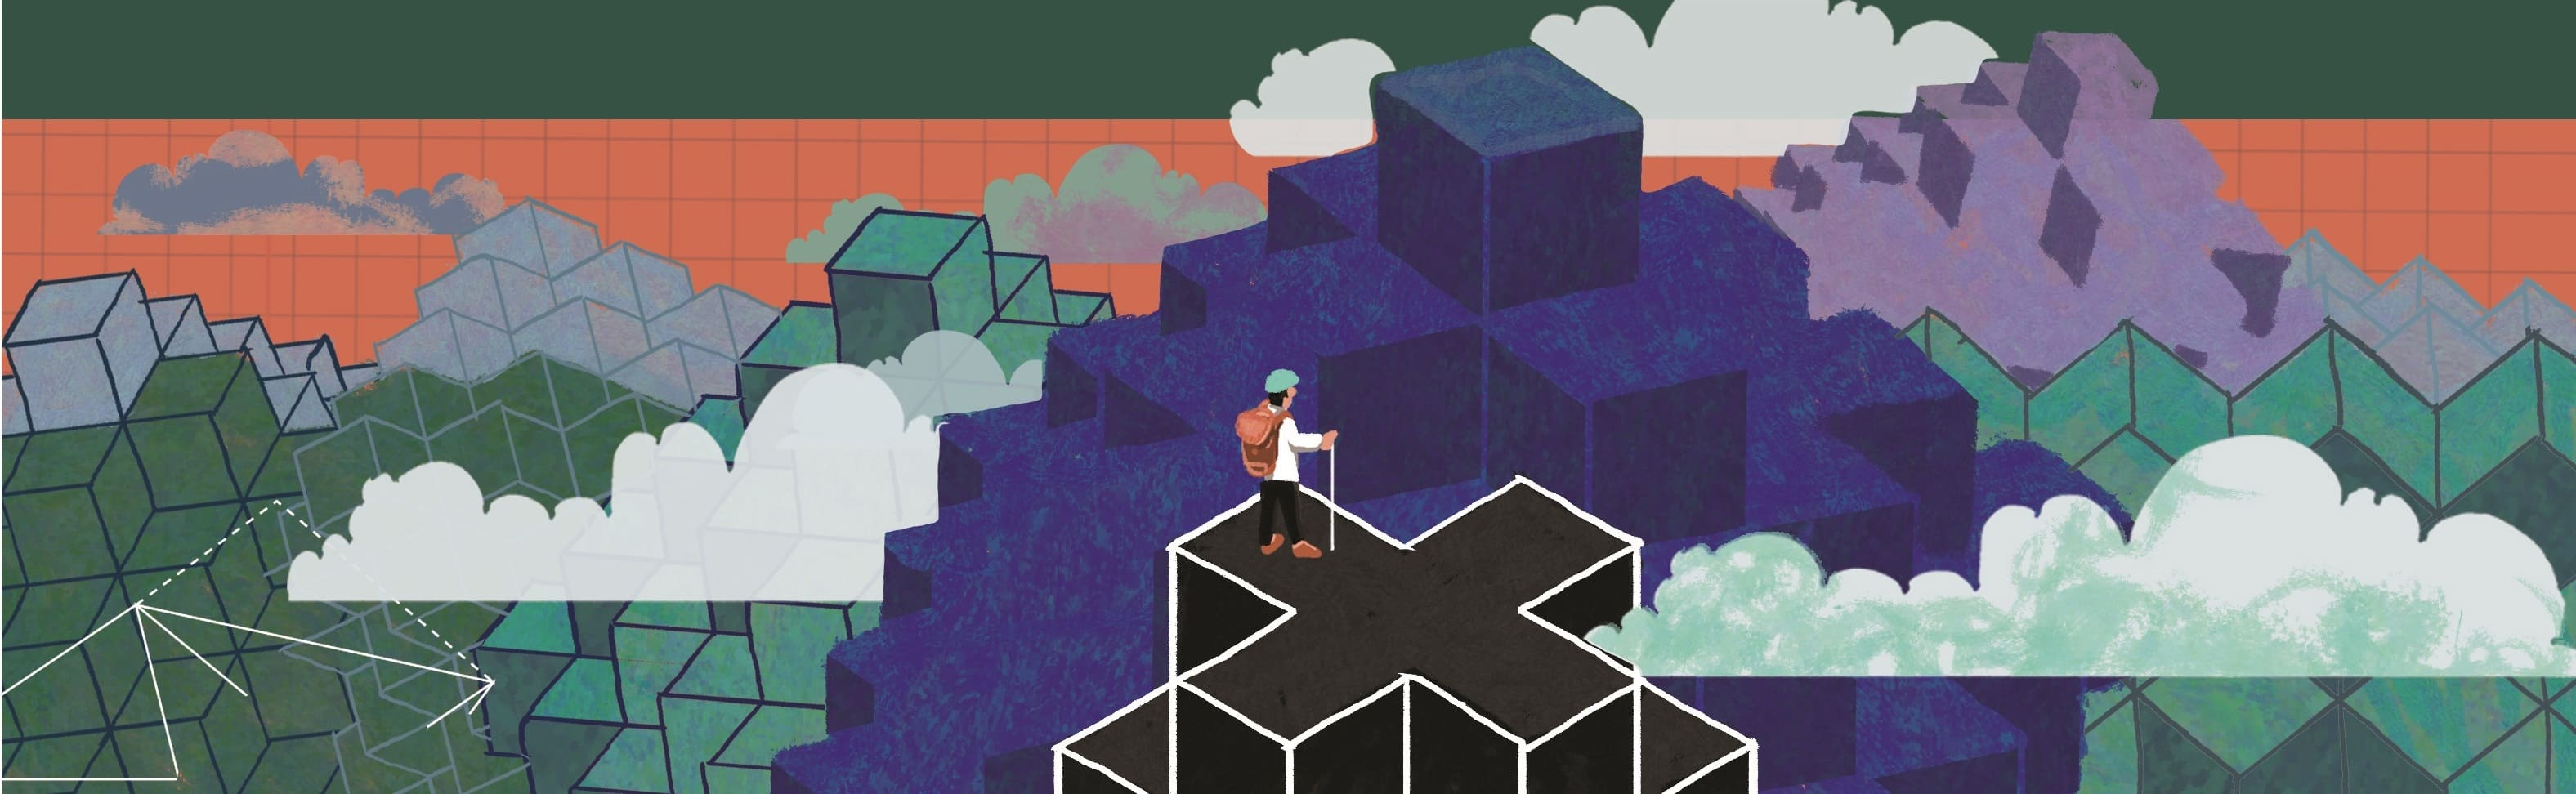
\includegraphics[width=19.3cm]{../thachthuctoanhoc/bannerthachthuc}}}
\centering
\vspace*{4cm}
\endgroup
\vspace*{-8pt}
\begin{tBox}
	\begin{itemize}[leftmargin = 13pt, itemsep = 1.0pt] 
		\item Mỗi bài toán đề xuất (kèm theo lời giải) cần được nêu rõ là bài sáng tác hay bài sưu tầm.
		%		\item Mỗi bài toán đề xuất (kèm theo lời giải) cần được nêu rõ là bài sáng tác hay bài sưu tầm (nếu là bài sưu tầm, cần ghi rõ nguồn).
		\item Bài giải cho mỗi bài toán cần được trình bày trong một file riêng hoặc
		một tờ giấy riêng.
		\item  Người đề xuất bài toán hoặc gửi bài giải cho các bài toán trong mục ``Thách thức kỳ này" cần ghi rõ họ, đệm, tên và nơi làm việc/học tập, số điện thoại liên hệ. Nếu là học sinh (hoặc sinh viên) cần ghi rõ là học sinh lớp mấy (hoặc sinh viên năm thứ mấy).
		\item Các bài toán trong mục Thách thức kỳ này hướng tới các độc giả là học sinh phổ thông; được phân chia thành các mức độ $B$, $A$, và được sắp xếp theo độ khó tăng dần, theo đánh giá chủ quan của Ban biên tập. Các bài toán mức độ $B$ không đòi hỏi các kiến thức vượt quá chương trình môn Toán cấp THCS; các bài toán mức độ $A$ không đòi hỏi các kiến thức vượt quá chương trình môn Toán cấp THPT.
		\item Cách thức gửi bài toán đề xuất hoặc lời giải: gửi file thu được bằng cách scan, ảnh chụp (rõ nét) của bản viết tay, hoặc được soạn thảo bằng các phần mềm Latex, Word tới \url{bbt@pi.edu.vn} hoặc gửi qua đường bưu điện tới Tòa soạn (xem địa chỉ tại bìa $2$).
		\item Hạn gửi lời giải cho các bài toán P$761$--P$770$: trước ngày $15/1/2024$.
	\end{itemize}
\end{tBox}
\begin{center}
	\vspace*{-5pt}
	\textbf{\color{thachthuctoanhoc}\color{thachthuctoanhoc}\color{thachthuctoanhoc}\color{thachthuctoanhoc}\color{thachthuctoanhoc}THÁCH THỨC KỲ NÀY}
	\vspace*{-5pt}
\end{center}
\begin{multicols}{2}
	\setlength{\abovedisplayskip}{4pt}
	\setlength{\belowdisplayskip}{4pt}
	{\color{thachthuctoanhoc}{\usefont{T5}{qag}{b}{n} P761.}}
	(Mức $B$) Mỗi  bạn An, Bình, Huệ, Nga đều có một món tiền tiết kiệm. Biết rằng tổng số tiền tiết kiệm của hai bạn bất kì trong $4$ bạn đó là $1900, 2070, 2110, 2330, 2500$ và $x$ nghìn đồng. Tìm $x$.
	\begin{flushright}
		\textit{Hoàng Việt Vương, Hà Nội}
	\end{flushright}
	{\color{thachthuctoanhoc}{\usefont{T5}{qag}{b}{n} P762.}}
	(Mức $B$) Cho đa giác đều có $2024$ đỉnh, tại mỗi đỉnh ta viết một số nguyên dương không vượt quá $1011$ (mỗi đỉnh viết một số). Chứng minh rằng tồn tại $4$ đỉnh $A,B,C,D$ của đa giác sao cho $ABCD$ là hình chữ nhật, và  $a+b=c+d$, trong đó $a,b,c,d$ tương ứng là các số lần lượt được viết tại các đỉnh $A,B,C,D$. 
	\begin{flushright}
		\textit{Nguyễn Đức Tấn, Tp. Hồ Chí Minh (st)}
	\end{flushright}
	{\color{thachthuctoanhoc}{\usefont{T5}{qag}{b}{n} P762.}}
	(Mức $B$) Cho tam giác $A B C$ có trọng tâm $G$. Dựng ra phía ngoài tam giác đó các tam giác $ABM$ và $ACN$ sao cho $\angle B A M=45^{\circ}$, $A B=3\sqrt2 A M$,  $\angle N A C=90^{\circ}$ và $A C=3 A N$. Chứng minh rằng $\angle G M N=90^{\circ}$.
	\begin{figure}[H]
		\vspace*{-10pt}
		\centering
		\captionsetup{labelformat= empty, justification=centering}
		\definecolor{qqzzcc}{rgb}{0,0.6,0.8}
		\definecolor{qqqqff}{rgb}{0,0,1}
		\definecolor{qqqqffa}{rgb}{1,1,1}
		\definecolor{cqcqcq}{rgb}{0.7529411764705882,0.7529411764705882,0.7529411764705882}
		\begin{tikzpicture}[thachthuctoanhoc,scale=0.58]
			\draw (-1.790333665478168,4.460157886210201) -- (-1.6004915516883682,4.669824220732033) -- (-1.8101578862102001,4.859666334521832) -- (-2,4.65) -- cycle; 
			\draw [shift={(-2,4.65)}] (0,0) -- (-151.55958953937227:0.7) arc (-151.55958953937227:-106.55958953937227:0.7) -- cycle;
			\draw [color=qqzzcc] (-2,4.65)-- (-3.68,-1);
			\draw [color=qqzzcc] (-3.68,-1)-- (4.24,-1);
			\draw [color=qqzzcc] (4.24,-1)-- (-2,4.65);
			\draw  (-3.2216666666666667,3.9883333333333337)-- (-3.68,-1);
			\draw  (-3.2216666666666667,3.9883333333333337)-- (-2,4.65);
			\draw  (-2,4.65)-- (-0.11666666666666714,6.73);
			\draw  (-0.11666666666666714,6.73)-- (4.24,-1);
			\draw  (-3.2216666666666667,3.9883333333333337)-- (-0.48,0.8833333333333334);
			\draw  (-0.48,0.8833333333333334)-- (-0.11666666666666714,6.73);
			\draw  (-0.11666666666666714,6.73)-- (-3.2216666666666667,3.9883333333333337);
			\draw (-2.65,4.55) node[anchor=north west] {\tiny$45^\circ$};
			\draw [fill = white] (-2,4.65) circle (1.5pt);
			\draw[color=qqqqff] (-2.12,5.08) node {$A$};
			\draw [fill = white] (-3.68,-1) circle (1.5pt);
			\draw[color=qqqqff] (-3.92,-1.36) node {$B$};
			\draw [fill = white] (4.24,-1) circle (1.5pt);
			\draw[color=qqqqff] (4.18,-1.36) node {$C$};
			\draw [fill = white] (-3.2216666666666667,3.9883333333333337) circle (1.5pt);
			\draw[color=qqqqff] (-3.54,4.34) node {$M$};
			\draw [fill = white] (-0.11666666666666714,6.73) circle (1.5pt);
			\draw[color=qqqqff] (0.04,7.04) node {$N$};
			\draw [fill = white] (-0.48,0.8833333333333334) circle (1.5pt);
			\draw[color=qqqqff] (-0.52,0.44) node {$G$};
		\end{tikzpicture}
		\vspace*{-15pt}
	\end{figure}
	\begin{flushright}
		\textit{Trần Việt Anh, Nam Định}
	\end{flushright}
	{\color{thachthuctoanhoc}{\usefont{T5}{qag}{b}{n} P764.}}
	(Mức $B$) Tìm tất cả các bộ ba số thực $(x,y,z)$, với $x,y,z\in\left(0,\frac12\right)$ và  thoả mãn 
	\begin{align*}
		\begin{cases}
			\left(3x^2+y^2\right)\sqrt{1-4z^2}\ge z&\\
			\left(3y^2+z^2\right)\sqrt{1-4x^2}\ge x&\\
			\left(3z^2+x^2\right)\sqrt{1-4y^2}\ge y.
		\end{cases}
	\end{align*}
	\begin{flushright}
		\textit{Ngô Văn Trang, Bắc Ninh}
	\end{flushright}
	{\color{thachthuctoanhoc}{\usefont{T5}{qag}{b}{n} P765.}}
	(Mức $B$) Cho số nguyên dương $n$. Gọi $A$ là tích tất cả các số nguyên dương không vượt quá $2n+1$, $B$ là tích tất cả các số nguyên dương lẻ không vượt quá $2n+1$ và $C$ là tích tất cả các số nguyên dương chẵn không vượt quá $2n$. Chứng minh rằng $4A+(B-C-1)^2$ không phải là số chính phương.
	\begin{flushright}
		\textit{Hà Duy Hưng, Hà Nội}
	\end{flushright}
	{\color{thachthuctoanhoc}{\usefont{T5}{qag}{b}{n} P766.}}
	(Mức $B$) Cho $a,b,c$ là các số dương. Chứng minh rằng
	\begin{align*}
		&\dfrac{a^2}{a^2+3ab+2b^2}+\dfrac{b^2}{b^2+3bc+2c^2}\\
		&+\dfrac{c^2}{c^2+3ca+2a^2}\ge \dfrac12.
	\end{align*}
	\begin{flushright}
		\textit{Ngô Văn Thái, Thái Bình}
	\end{flushright}
	{\color{thachthuctoanhoc}{\usefont{T5}{qag}{b}{n} P767.}}
	(Mức $A$) Cho $x,y,z$ là các số thực không âm thoả mãn $x^2+y^2+z^2=3$. Chứng minh rằng
	\begin{align*}
		&3(x+y+x+xyz)\\
		\ge\, &4\sqrt{(x^2+yz)(y^2+zx)(z^2+xy)}.
	\end{align*}
	\begin{flushright}
		\textit{Hoàng Ngọc Minh, Hà Nội}
	\end{flushright}
	{\color{thachthuctoanhoc}{\usefont{T5}{qag}{b}{n} P768.}}
	(Mức $A$) Cho $a$ là một số nguyên dương lẻ và không phải là số chính phương. Chứng minh rằng
	\begin{align*}
		\left[m(a+\sqrt a)\right]\ne \left[n(a-\sqrt a)\right]
	\end{align*}
	với mọi số nguyên dương $m,n$. 
	\begin{flushright}
		\textit{Nguyễn Hoàng Duy, Thái Bình (st)}
	\end{flushright}
	\vskip 0.1cm
	\columnbreak
	{\color{thachthuctoanhoc}{\usefont{T5}{qag}{b}{n} P769.}}
	(Mức $A$) Cho tam giác không cân $ABC$ nội tiếp đường tròn $(O)$. $K$ là một điểm (khác $A$) trên tiếp tuyến tại $A$ của $(O)$. $\Delta$ là một đường thẳng đi qua $K$, cắt $BC, CA, AB$ lần lượt tại $D, E, F$. Chứng minh rằng tâm đẳng phương của các đường tròn: đường tròn đường kính $EF$, đường tròn đường kính $DK$, đường tròn $(O)$ thuộc đường thẳng $\Delta.$
	\begin{center}
		\definecolor{qqqqff}{rgb}{0,0,1}
		\definecolor{qqqqffa}{rgb}{1,1,1}
		\definecolor{cqcqcq}{rgb}{0.7529411764705882,0.7529411764705882,0.7529411764705882}
		\begin{tikzpicture}[thachthuctoanhoc, scale=0.54]
			\draw  (-4.38,5.01)-- (-5.56,-0.3);
			\draw  (-5.56,-0.3)-- (1.58,-0.3);
			\draw  (1.58,-0.3)-- (-4.38,5.01);
			\draw  (-1.99,1.6927777777777777) circle (4.08852825251397cm);
			\draw  (-7.256570958905223,2.93748144947073)-- (5.1899690781026155,-0.3);
			\draw  (1.58,-0.3)-- (5.1899690781026155,-0.3);
			\draw  (-7.256570958905223,2.93748144947073)-- (-4.38,5.01);
			\draw [fill = white] (-4.38,5.01) circle (1.5pt);
			\draw[color=qqqqff] (-4.44,5.5) node {$A$};
			\draw [fill = white] (-5.56,-0.3) circle (1.5pt);
			\draw[color=qqqqff] (-5.94,-0.5) node {$B$};
			\draw [fill = white] (1.58,-0.3) circle (1.5pt);
			\draw[color=qqqqff] (1.7,-0.73) node {$C$};
			\draw [fill = white] (-7.256570958905223,2.93748144947073) circle (1.5pt);
			\draw[color=qqqqff] (-7.72,3.06) node {$K$};
			\draw [fill = white] (5.1899690781026155,-0.3) circle (1.5pt);
			\draw[color=qqqqff] (5.14,-0.73) node {$D$};
			\draw [fill = white] (0.09149352555368925,1.0261693589446155) circle (1.5pt);
			\draw[color=qqqqff] (0.2,1.52) node {$E$};
			\draw [fill = white] (-4.972579921493512,2.343390353279194) circle (1.5pt);
			\draw[color=qqqqff] (-5.22,2.8) node {$F$};
		\end{tikzpicture}
	\end{center}
	\begin{flushright}
		\textit{Lưu Công Đông, Hà Nội}
	\end{flushright}
	{\color{thachthuctoanhoc}{\usefont{T5}{qag}{b}{n} P770.}}
	(Mức $A$) Cho phép thực hiện việc đổi chỗ các số hạng trong một hoán vị, theo qui tắc: Mỗi lần, lấy ra khỏi hoán vị tám số hạng tùy ý của nó, rồi lại xếp tám số hạng đó vào tám vị trí mà chúng đã nằm, nhưng theo thứ tự ngược lại.
	Hỏi, nhờ việc thực hiện liên tiếp một số hữu hạn lần phép đổi chỗ nói trên đối với hoán vị $(1,2,\ldots,2023)$ của $2023$ số nguyên dương đầu tiên, ta có thể nhận được hoán vị $(2023,2022,\ldots,1)$ hay không?
	\begin{flushright}
		\textit{Nguyễn Khắc Minh, Hà Nội}
	\end{flushright}
\end{multicols}
\newpage
\centerline{{\large{\textbf{\color{thachthuctoanhoc}\color{thachthuctoanhoc}\color{thachthuctoanhoc}GIẢI BÀI KỲ TRƯỚC}}}}
\vspace*{-5pt}
\begin{multicols}{2}
	\setlength{\abovedisplayskip}{5pt}
	\setlength{\belowdisplayskip}{5pt}
	{\color{thachthuctoanhoc}{\usefont{T5}{qag}{b}{n} P731.}}
	(Mức $B$) Ghép chín hình vuông thành một hình chữ nhật, như ở hình dưới đây. Biết rằng, hình vuông màu đen có cạnh bằng $1$. Tìm chiều dài và chiều rộng của hình chữ nhật.
	\begin{figure}[H]
		\vspace*{-5pt}
		\centering
		\captionsetup{labelformat= empty, justification=centering}
		\begin{tikzpicture}[thachthuctoanhoc,scale=0.15]
			\draw[fill=black] (0,0) rectangle (1,1);
			\draw  (0.,-9.)-- (9.,-9.);
			\draw  (9.,-9.)-- (9.,0.);
			\draw  (9.,0.)-- (0.,0.);
			\draw  (0.,0.)-- (0.,-9.);
			\draw  (1.,0.)-- (9.,0.);
			\draw  (9.,0.)-- (9.,8.);
			\draw  (9.,8.)-- (1.,8.);
			\draw  (1.,8.)-- (1.,0.);
			\draw  (-10.,-9.)-- (0.,-9.);
			\draw  (0.,-9.)-- (0.,1.);
			\draw  (0.,1.)-- (-10.,1.);
			\draw  (-10.,1.)-- (-10.,-9.);
			\draw  (-6.,1.)-- (1.,1.);
			\draw  (1.,1.)-- (1.,8.);
			\draw  (1.,8.)-- (-6.,8.);
			\draw  (-6.,8.)-- (-6.,1.);
			\draw  (-10.,1.)-- (-6.,1.);
			\draw  (-6.,1.)-- (-6.,5.);
			\draw  (-6.,5.)-- (-10.,5.);
			\draw  (-10.,5.)-- (-10.,1.);
			\draw  (-6.,8.)-- (9.,8.);
			\draw  (9.,8.)-- (9.,23.);
			\draw  (9.,23.)-- (-6.,23.);
			\draw  (-6.,23.)-- (-6.,8.);
			\draw  (-24.,-9.)-- (-10.,-9.);
			\draw  (-10.,-9.)-- (-10.,5.);
			\draw  (-10.,5.)-- (-24.,5.);
			\draw  (-24.,5.)-- (-24.,-9.);
			\draw  (-24.,5.)-- (-6.,5.);
			\draw  (-6.,5.)-- (-6.,23.);
			\draw  (-6.,23.)-- (-24.,23.);
			\draw  (-24.,23.)-- (-24.,5.);	
		\end{tikzpicture}
		\vspace*{-10pt}
	\end{figure} 
	\textbf{\color{thachthuctoanhoc}Lời giải} \textit{(dựa theo tất cả lời giải Tạp chí đã nhận được từ bạn đọc})\textbf{\color{thachthuctoanhoc}.}
	\vskip 0.05cm
	Đặt tên các hình vuông như ở hình vẽ dưới đây:
	\begin{figure}[H]
		\vspace*{-5pt}
		\centering
		\captionsetup{labelformat= empty, justification=centering}
		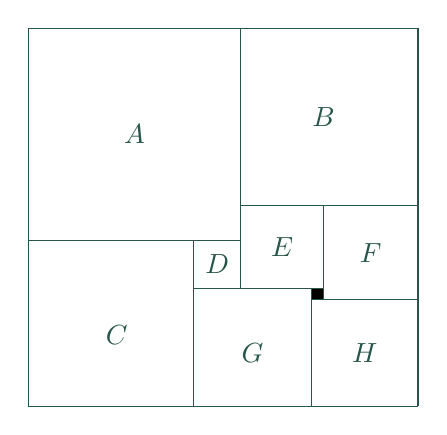
\begin{tikzpicture}[thachthuctoanhoc,scale=0.15]
			\draw[fill=black] (0,0) rectangle (1,1);
			\draw  (0.,-9.)-- (9.,-9.);
			\draw  (9.,-9.)-- (9.,0.);
			\draw (4.5,-4.5) node {$H$};
			\draw (5,4) node {$F$};
			\draw (-2.5,4.5) node {$E$};
			\draw (-5,-4.5) node {$G$};
			\draw (-8,3) node {$D$};
			\draw (1,15.5) node {$B$};
			\draw (-15,14) node {$A$};
			\draw (-16.5,-3) node {$C$};
			\draw  (9.,0.)-- (0.,0.);
			\draw  (0.,0.)-- (0.,-9.);
			\draw  (1.,0.)-- (9.,0.);
			\draw  (9.,0.)-- (9.,8.);
			\draw  (9.,8.)-- (1.,8.);
			\draw  (1.,8.)-- (1.,0.);
			\draw  (-10.,-9.)-- (0.,-9.);
			\draw  (0.,-9.)-- (0.,1.);
			\draw  (0.,1.)-- (-10.,1.);
			\draw  (-10.,1.)-- (-10.,-9.);
			\draw  (-6.,1.)-- (1.,1.);
			\draw  (1.,1.)-- (1.,8.);
			\draw  (1.,8.)-- (-6.,8.);
			\draw  (-6.,8.)-- (-6.,1.);
			\draw  (-10.,1.)-- (-6.,1.);
			\draw  (-6.,1.)-- (-6.,5.);
			\draw  (-6.,5.)-- (-10.,5.);
			\draw  (-10.,5.)-- (-10.,1.);
			\draw  (-6.,8.)-- (9.,8.);
			\draw  (9.,8.)-- (9.,23.);
			\draw  (9.,23.)-- (-6.,23.);
			\draw  (-6.,23.)-- (-6.,8.);
			\draw  (-24.,-9.)-- (-10.,-9.);
			\draw  (-10.,-9.)-- (-10.,5.);
			\draw  (-10.,5.)-- (-24.,5.);
			\draw  (-24.,5.)-- (-24.,-9.);
			\draw  (-24.,5.)-- (-6.,5.);
			\draw  (-6.,5.)-- (-6.,23.);
			\draw  (-6.,23.)-- (-24.,23.);
			\draw  (-24.,23.)-- (-24.,5.);	
		\end{tikzpicture}
		\vspace*{-10pt}
	\end{figure} 
	Gọi $a, b, c, d, e, g, h$ tương ứng là độ dài cạnh của các hình vuông $A, B, C, D, E, G, H$.
	\vskip 0.1cm
	Gọi $x$ là độ dài cạnh của hình vuông $F$.
	\vskip 0.1cm
	Khi đó, do hình vuông màu đen có cạnh bằng $1$, nên
	\begin{align*}
		&e = x - 1; b = e + x = 2x - 1;\\
		&h = x + 1; g = h + 1 = x + 2;\\
		&d = g - (e - 1) = (x + 2) - (x - 2) = 4;\\
		&c = g + d = (x + 2) + 4 = x + 6;\\
		&a = c + d = (x + 6) + 4 = x + 10.
	\end{align*}
	Từ đó, do $a + c = b + x + h$, nên ta có:
	\begin{align*}
		(x + 10) + (x + 6) = (2x - 1) + x + (x + 1).
	\end{align*}
	Suy ra, $2x + 16 = 4x$. Do đó, $x = 8$. Suy ra
	\begin{align*}
		&a = 8 + 10 = 18, b = 2\cdot8 - 1 = 15 \\
		\text{ và } &c = 8 + 6 = 14.
	\end{align*}
	Vì vậy, hình chữ nhật có chiều dài là:
	\begin{align*}
		18 + 15 = 33,
	\end{align*}
	và chiều rộng là: $18 + 14 = 32$.
	\vskip 0.05cm
	\textbf{\color{thachthuctoanhoc}Bình luận và Nhận xét}
	\vskip 0.05cm	
	Tất cả lời giải Tạp chí đã nhận được từ bạn đọc đều là lời giải đúng và hoàn chỉnh.
	\begin{flushright}
		\textbf{\color{thachthuctoanhoc}Hà Thanh}
	\end{flushright}
	{\color{thachthuctoanhoc}{\usefont{T5}{qag}{b}{n} P732.}}
	(Mức $B$) Xét bốn số thực (không nhất thiết đôi một khác nhau), mà mỗi số có trị tuyệt đối không vượt quá $\dfrac{1}{2}$, và tổng của ba số bất kỳ, trong bốn số đó, là một số nguyên. Tìm tất cả các giá trị có thể của tổng bốn số đó.
	\vskip 0.05cm
	\textbf{\color{thachthuctoanhoc}Lời giải} (\textit{phỏng theo cách giải của bạn Ngô Minh Chấn, lớp $9$A$3$, trường TH$\&$THCS Archimedes Đông Anh, Tp. Hà Nội})\textbf{\color{thachthuctoanhoc}.}
	\vskip 0.05cm
	Gọi $a, b, c, d$ là bốn số thực thỏa mãn các điều kiện đã nêu trong đề bài.
	\vskip 0.05cm
	Đặt $x = a \!+\! b \!+\! c$, $y = a \!+\! b \!+\! d$, $z = a \!+\! c \!+\! d$, $t = b + c + d$, và
	$s = a + b + c + d$.
	\vskip 0.05cm
	Khi đó, theo giả thiết của bài ra, ta có:
	\begin{align*}
		|a| \le \frac{1}{2}, |b| \le \frac{1}{2},|c| \le \frac{1}{2},|d| \le \frac{1}{2}; \tag{$1$}
	\end{align*}
	và $x, y, z, t$ là các số nguyên.        \hfill ($2$)
	\vskip 0.05cm
	Xét cặp số $x, y$.
	Do ($2$) nên $x - y$ là một số nguyên; hơn nữa
	\begin{align*}
		\left| {x - y} \right| &= \left| {c - d} \right| \le |c| + \left| {d} \right| \\
		&\le 1 \quad\text{(do ($1$))}. \tag{$3$}
	\end{align*}
	Vì thế, $\left| {x - y} \right| \in \left\{ {0;1} \right\}.$ \hfill ($4$)
	\vskip 0.05cm
	Nếu $|x - y| = 1$  thì theo ($3$), phải có:
	\begin{align*}
		\left| {c - d} \right| = |c| + \left| {d} \right| = 1.
	\end{align*}
	Điều vừa nêu trên tương đương với
	\begin{align*}
	\quad\quad	\begin{cases}
			cd \le 0\\
			|c| = |d| = \dfrac{1}{2} \text{ (do ($1$)).} \quad\quad\quad\quad \text{($5$)} 
		\end{cases}
	\end{align*}
	Suy ra, $c + d = 0$. Do đó, $z = a$ và $t = b$. Vì thế, $a,b \in \mathbb{Z}$  (do ($2$)). Từ đây và ($1$), suy ra $a = b = 0$.
	\vskip 0.05cm
	Vì vậy, $x = c$. Do đó,  $c \in \mathbb{Z}$. Từ đây và ($1$), suy ra $c = 0$, mâu thuẫn với ($5$).
	\vskip 0.05cm
	Mâu thuẫn nhận được ở trên cho thấy
	\begin{align*}
		|x - y| \ne 1.
	\end{align*}
	Do đó, từ ($4$) ta được $x = y$.
	\vskip 0.05cm
	Xét các cặp số $x, z$ và $x, t$, bằng cách hoàn toàn tương tự, ta sẽ được $x = z$ và $x = t$.
	\vskip 0.05cm
	Vì vậy, $x = y = z = t$. Suy ra
	\begin{align*}
		3s = x  + y + z + t = 4x;
	\end{align*}
	do đó, $s = \dfrac{4}{3}x$. \hfill ($6$)
	\vskip 0.05cm
	Tiếp theo, ta có:
	\begin{align*}
		|x| \le |a| + |b| + |c| \le \frac{3}{2} \quad\text{(do ($1$))}; 
	\end{align*}
	mà $|x| \in \mathbb{Z}$  (theo ($2$)), nên  $|x| \in \{0;1\}$. \hfill ($7$)
	\vskip 0.05cm
	Từ ($6$) và ($7$), suy ra $s \in \{-\dfrac{4}{3}; 0; \dfrac{4}{3}\}$.
	\vskip 0.05cm 
	Ngược lại, dễ thấy:
	\vskip 0.05cm
	$\bullet$ $a=b=c=d = -\dfrac{1}{3}$   là bốn số thực thỏa mãn các điều kiện của đề bài, và có tổng bằng $- \dfrac{4}{3}$;
	\vskip 0.05cm  
	$\bullet$  $a=b=c=d = 0$  là bốn số thực thỏa mãn các điều kiện của đề bài, và có tổng bằng $0$;
	\vskip 0.05cm
	$\bullet$ $a=b=c=d = \dfrac{1}{3}$   là bốn số thực thỏa mãn các điều kiện của đề bài, và có tổng bằng $\dfrac{4}{3}$;
	\vskip 0.05cm  
	Vậy, tất cả các giá trị có thể của tổng bốn số thỏa mãn các điều kiện của đề bài là:  $- \dfrac{4}{3}, 0, \dfrac{4}{3}$.
	\vskip 0.05cm  
	\textbf{\color{thachthuctoanhoc}Bình luận và Nhận xét}
	\vskip 0.05cm
	$\pmb{1.}$ Lời giải trên cho thấy, các bộ bốn số thực được liệt kê ở phần cuối của Lời giải là \textit{tất cả} các bộ bốn số thực thỏa mãn các điều kiện của đề bài.
	\vskip 0.05cm
	$\pmb{2.}$ Trong số các lời giải Tạp chí đã nhận được từ bạn đọc, rất tiếc, có hai lời giải sai, do người giải bài hoặc mới chỉ ra điều kiện cần (nhưng không đủ) cho giá trị của tổng bốn số đã vội kết luận đó là các giá trị có thể của tổng đó, hoặc đã chỉ ra sai các bộ bốn số thực thỏa mãn các điều kiện của đề bài. Bên cạnh đó, còn có một lời giải chưa đầy đủ, do người giải bài chưa xét hết các trường hợp có thể xảy~ra.
	\begin{flushright}
		\textbf{\color{thachthuctoanhoc}Hà Thanh}
	\end{flushright}
	{\color{thachthuctoanhoc}{\usefont{T5}{qag}{b}{n} P733.}}
	(Mức $B$)
	Tìm giá trị nhỏ nhất của biểu thức
	\begin{align*}
		S = \left\lfloor {\frac{{b + c}}{a}} \right\rfloor  + \left\lfloor {\frac{{c + a}}{b}} \right\rfloor  + \left\lfloor {\frac{{a + b}}{c}} \right\rfloor ,
	\end{align*}
	trong đó, $a, b, c$ là các biến nguyên dương.
	($\left\lfloor x \right\rfloor $  ký hiệu số nguyên lớn nhất không vượt quá $x$.)
	\vskip 0.05cm
	\textbf{\color{thachthuctoanhoc}Lời giải} (\textit{dựa theo lời giải của các bạn: Ngô Minh Chấn, lớp $9$A$3$, trường TH$\&$THCS Archimedes Đông Anh, Tp. Hà Nội; Lê Nguyễn Hoàng Nhật Đình, lớp $9$C, trường THCS Nguyễn Thái Bình, tỉnh Cà Mau; Trương Anh Dũng, lớp $10$A$1$ chuyên Toán, trường THPT chuyên Vĩnh Phúc, tỉnh Vĩnh Phúc})\textbf{\color{thachthuctoanhoc}.}
	\vskip 0.05cm
	Từ định nghĩa phần nguyên của một số thực dễ thấy, với mọi số thực $x$, ta đều có
	\begin{align*}
		\left\lfloor x \right\rfloor  > x -1.
	\end{align*}
	Vì vậy, với lưu ý $a, b, c$ là các số dương, ta có:
	\begin{align*}
			S &> \frac{{b + c}}{a} + \frac{{c + a}}{b} + \frac{{a + b}}{c} - 3 \\
			&= \left( {\frac{b}{a} + \frac{a}{b}} \right) + \left( {\frac{c}{a} + \frac{a}{c}} \right) + \left( {\frac{c}{b} + \frac{b}{c}} \right) - 3\\
			 &\ge 2\sqrt {\frac{b}{a} \!\cdot\! \frac{a}{b}}  \!+\! 2\sqrt {\frac{c}{a} \!\cdot\! \frac{a}{c}}  \!+\! 2\sqrt {\frac{c}{b} \!\cdot\! \frac{b}{c}}  \!-\! 3 \!=\! 3.
	\end{align*}
	Từ đó, do $S$ là số nguyên, suy ra $S \ge 4$.
	\vskip 0.05cm
	Hơn nữa, dễ thấy, với $a = 3, b = c = 4$, ta có $S = 4$.
	\vskip 0.05cm
	Vì vậy, giá trị nhỏ nhất của $S$ bằng $4$.
	\vskip 0.05cm
	\textbf{\color{thachthuctoanhoc}Bình luận và Nhận xét}
	\vskip 0.05cm
	$\pmb{1.}$ Lời giải trên cho thấy, kết quả của bài ra không thay đổi, khi thay giả thiết ``$a, b, c$ là các biến nguyên dương" bởi giả thiết ``$a, b, c$ là các biến thực dương".
	\vskip 0.05cm
	$\pmb{2.}$ Trong số các lời giải Tạp chí đã nhận được từ bạn đọc, rất tiếc, có một lời giải sai, do người giải bài đã mắc sai sót về kiến thức cơ bản, khi khẳng định ``$\left\lfloor x \right\rfloor  \ge x$  với mọi số thực $x$".
	\begin{flushright}
		\textbf{\color{thachthuctoanhoc}Lưu Thị Thanh Hà}
	\end{flushright}
	{\color{thachthuctoanhoc}{\usefont{T5}{qag}{b}{n} P734.}}
	(Mức $B$) Cho hình vuông $ABCD$. Gọi $E$ là trung điểm của $AD$; $H$ là hình chiếu vuông góc của $B$ trên $CE$. Trên đường chéo $AC$, lấy điểm $M$ sao cho $AM = \dfrac{3}{8}AC$. Chứng minh rằng, $ME$ song song với $DH$.
	\vskip 0.05cm
	\textbf{\color{thachthuctoanhoc}Lời giải} (\textit{dựa theo lời giải của bạn Nguyễn Nguyên Chinh, lớp $9$D, trường THCS Nguyễn Chí Thanh, tỉnh Phú Yên})\textbf{\color{thachthuctoanhoc}.}
	\begin{figure}[H]
		\vspace*{-5pt}
		\centering
		\captionsetup{labelformat= empty, justification=centering}
		\definecolor{qqwuqq}{rgb}{0.,0.39215686274509803,0.}
		\definecolor{uuuuuu}{rgb}{0.26666666666666666,0.26666666666666666,0.26666666666666666}
		\definecolor{qqqqff}{rgb}{0.,0.,1.}
		\begin{tikzpicture}[thachthuctoanhoc,scale=0.45]
			\draw [shift={(10.,5.)},pattern color=qqwuqq,fill=qqwuqq,fill opacity=0.10000000149011612] (0,0) -- (-116.56505117707799:0.8153190950798923) arc (-116.56505117707799:-90.:0.8153190950798923) -- cycle;
			\draw [shift={(10.,-4.)},pattern color=qqwuqq,fill=qqwuqq,fill opacity=0.10000000149011612] (0,0) -- (153.43494882292202:0.8153190950798923) arc (153.43494882292202:180.:0.8153190950798923) -- cycle;
			\draw[pattern color=qqwuqq,fill=qqwuqq,fill opacity=0.10000000149011612] (6.743768714703979,-2.3718843573519894) -- (6.915653072055969,-2.028115642648011) -- (6.57188435735199,-1.8562312852960212) -- (6.4,-2.2) -- cycle; 
			\draw[pattern color=qqwuqq,fill=qqwuqq,fill opacity=0.10000000149011612] (1.3843451073079143,-4.) -- (1.3843451073079143,-3.6156548926920857) -- (1.,-3.6156548926920857) -- (1.,-4.) -- cycle; 
			\draw  (1.,5.)-- (10.,5.);
			\draw  (1.,-4.)-- (10.,-4.);
			\draw  (10.,-4.)-- (10.,5.);
			\draw  (1.,5.)-- (10.,-4.);
			\draw [color=qqqqff] (1.,0.5)-- (4.375,1.625);
			\draw  (1.,0.5)-- (10.,-4.);
			\draw [color=qqqqff] (6.4,-2.2)-- (1.,-4.);
			\draw  (6.4,-2.2)-- (10.,5.);
			\draw  (1.,-7.)-- (1.,-4.);
			\draw [color=qqqqff] (1.,-7.)-- (10.,-4.);
			\draw (-0.44481130622791615,6.007702325581402) node[anchor=north west] {$A$};
			\draw (10.011222021831985,6.134879628750732) node[anchor=north west] {$B$};
			\draw (10.038399325001315,-3.477176480514691) node[anchor=north west] {$C$};
			\draw (-0.2002155777039485,-3.341289964668042) node[anchor=north west] {$D$};
			\draw (-0.2002155777039485,1.1157877551020416) node[anchor=north west] {$E$};
			\draw (5.934626546432524,-2.20639567157095424) node[anchor=north west] {$H$};
			\draw (4.30398835627274,2.55618482307652) node[anchor=north west] {$M$};
			\draw (0.44481130622791615,-6.92807467172924) node[anchor=north west] {$N$};
			\draw  (1.,0.5)-- (1.,5.);
			\draw  (0.8777021357380159,2.7024397194536727) -- (1.1222978642619836,2.7024397194536727);
			\draw  (0.8777021357380159,2.797560280546327) -- (1.1222978642619836,2.797560280546327);
			\draw  (1.,0.5)-- (1.,-4.);
			\draw  (1.1222978642619836,-1.7024397194536725) -- (0.8777021357380159,-1.7024397194536725);
			\draw  (1.1222978642619836,-1.7975602805463267) -- (0.8777021357380159,-1.7975602805463267);
				\draw [fill=qqqqff] (1.,5.) circle (1.5pt);
				\draw [fill=qqqqff] (10.,5.) circle (1.5pt);
				\draw [fill=qqqqff] (10.,-4.) circle (1.5pt);
				\draw [fill=qqqqff] (1.,-4.) circle (1.5pt);
				\draw [fill=uuuuuu] (1.,0.5) circle (1.5pt);
				\draw [fill=qqqqff] (4.375,1.625) circle (1.5pt);
				\draw [fill=uuuuuu] (6.4,-2.2) circle (1.5pt);
				\draw [fill=uuuuuu] (1.,-7.) circle (1.5pt);
		\end{tikzpicture}
		\vspace*{-10pt}
	\end{figure}
	Qua $C$, kẻ đường thẳng song song với $ME$, cắt đường thẳng $AD$ tại $N$.
	\vskip 0.05cm
	Khi đó, theo định lý Thales, ta có:
	\begin{align*}
		\frac{{AN}}{{AE}} = \frac{{AC}}{{AM}} = \frac{8}{3} \quad\text{(theo giả thiết).}
	\end{align*}
	Từ đó, với lưu ý $E$ là trung điểm của $AD$ (giả thiết), suy ra
	\begin{align*}
		\frac{{DN}}{{DE}} = \frac{{DN}}{{AE}} = \frac{{AN}}{{AE}} - \frac{{AD}}{{AE}} = \frac{8}{3} - 2 = \frac{2}{3}.
	\end{align*}
	Do đó
	\begin{align*}
		\frac{{NE}}{{ND}} &= \frac{{ND + DE}}{{ND}} = 1 + \frac{{DE}}{{ND}} \\
		&= 1 + \frac{3}{2} = \frac{5}{2}. \tag{$1$}
	\end{align*}
	Đặt $AD = a$. Từ giả thiết của bài ra, ta có $CD = a$ và
	\begin{align*}
		AE = \frac{{AD}}{2} = \frac{a}{2}.
	\end{align*}
	Vì vậy, áp dụng định lý Pithagoras cho tam giác vuông $CDE$, ta được:
	\begin{align*}
		C{E^2} &= C{D^2} + D{E^2} \\
		&= {a^2} + {\left( {\frac{a}{2}} \right)^2} = \frac{5}{4}{a^2}. \tag{$2$}
	\end{align*}
	Tiếp theo, do
	\begin{align*}
		\angle CBH = {90^{\rm{o}}} - \angle BCH = \angle DCE,
	\end{align*}
	nên tam giác vuông $BHC$ đồng dạng với tam giác vuông $CDE$. Do đó
	\begin{align*}
		\frac{{CH}}{{CB}} = \frac{{ED}}{{EC}};
	\end{align*}
	suy ra
	\begin{align*}
			\frac{{CH}}{{CE}} = \frac{{ED \cdot CB}}{{C{E^2}}} = \frac{{\dfrac{a}{2} \cdot a}}{{\dfrac{5}{4}{a^2}}}\quad\left( {{\rm{theo}}(2)} \right)\\
			 = \frac{2}{5} = \frac{{ND}}{{NE}}\quad\left( {{\rm{theo}}(1)} \right).
	\end{align*}
	Do đó, $DH \parallel NC$ (theo định lý Thales); mà $NC \parallel ME$, nên $DH \parallel ME$.
	\vskip 0.05cm
	Ta có điều phải chứng minh theo yêu cầu đề bài. 
	\vskip 0.05cm
	\textbf{\color{thachthuctoanhoc}Bình luận và Nhận xét}
	\vskip 0.05cm
	Trong số các lời giải Tạp chí đã nhận được từ bạn đọc, có một lời giải bằng phương pháp tọa độ. Rất tiếc, lời giải này được diễn đạt rất sai bằng ngôn ngữ Toán học; và vì thế, không thể coi là lời giải đúng.
	\begin{flushright}
		\textbf{\color{thachthuctoanhoc}Hạ Vũ Anh}
	\end{flushright}
	{\color{thachthuctoanhoc}{\usefont{T5}{qag}{b}{n} P735.}}
	(Mức $B$) Tìm tất cả các số nguyên dương $n$, để $n! + n$ là một lũy thừa với số mũ nguyên dương của một số nguyên tố.
	\vskip 0.05cm
	\textbf{\color{thachthuctoanhoc}Lời giải} (\textit{dựa theo đa số lời giải Tạp chí đã nhận được từ bạn đọc})\textbf{\color{thachthuctoanhoc}.}
	\vskip 0.05cm
	$\bullet$ Giả sử $n$ là số nguyên dương thỏa mãn yêu cầu đề bài.
	\vskip 0.05cm
	Khi đó, tồn tại số nguyên tố $p$ và số nguyên dương $\alpha$, sao cho
	\begin{align*}
		n! + n = {p^\alpha },
	\end{align*}
	hay  
	\begin{align*}
		n\left( {\left( {n - 1} \right)! + 1} \right) = {p^\alpha }. \tag{$1$}
	\end{align*}
	Do $\left( {n - 1} \right)! + 1 > 1$  nên từ ($1$) suy ra, tồn tại số tự nhiên $\beta < \alpha$, sao cho $n = p^{\beta}$  và
	\begin{align*}
		\left( {n - 1} \right)! + 1 = {p^{\alpha  - \beta }}. \tag{$2$}
	\end{align*}
	Vì  $\beta \in  \mathbb{N}, \alpha \in \mathbb{N^*}$   và $\beta < \alpha$, nên  $\alpha - \beta$ là một số nguyên dương. Do đó, từ ($2$) suy ra
	\begin{align*}
		\left( {n - 1} \right)! + 1 \equiv 0\left( {\bmod p} \right). \tag{$3$}
	\end{align*}
	Từ ($2$) và ($3$) suy ra $\beta \in \{0;1\}$, vì nếu ngược lại, $\beta \ge 2$,  thì
	\begin{align*}
		n - 1 \ge {p^2} - 1 > p \text{ (do $n = p^{\beta}$  và $p \ge 2$)};
	\end{align*}
	dẫn tới $\left( {n - 1} \right)! \,\,\vdots\,\, p,$  và do đó,  $1 \,\,\vdots\,\, p$ (theo ($3$)), là điều vô lý.
	\vskip 0.05cm
	Với $\beta= 0$, ta có $n = p^0 = 1$. \hfill ($4$)
	\vskip 0.05cm
	Với $\beta = 1$, ta có $n = p$; do đó
	\begin{align*}
		\left( {p - 1} \right)! + 1 = {p^{\alpha  - 1}}	\quad\text{(theo ($2$))}. \tag{$5$}
	\end{align*}                                                      
	Xét $p > 5$. Khi đó
	\begin{align*}
		\left( {p - 1} \right)! > \left( {p - 1} \right)\left( {p - 2} \right) > p.
	\end{align*}
	Vì thế, từ ($5$) suy ra $\alpha -1\ge 2$, hay $\alpha \ge 3$. Do vậy, từ ($5$) ta có:
	\begin{align*}
		&\left( {p - 1} \right)! = {p^{\alpha  - 1}} - 1 \\
		=\, &\left( {p - 1} \right)\left( {{p^{\alpha  - 2}} + {p^{\alpha  - 3}} +  \cdots  + p + 1} \right).
	\end{align*}
	Suy ra
	\begin{align*}
		\left( {p \!-\! 2} \right)! \!=\! {p^{\alpha  \!-\! 2}} \!+\! {p^{\alpha  \!-\! 3}} \!+\!  \cdots  \!+\! p \!+\! 1. \tag{$6$}
	\end{align*}
	Tiếp theo, do $p$ là số nguyên tố lớn hơn $5$ nên $p - 1$ là một hợp số lớn hơn $4$. Vì thế, tồn tại các số nguyên dương $a, b$, với $1 < a \le b$, sao cho $p - 1 = ab$.
	\vskip 0.05cm
	-- Nếu $a = b$ thì
	\begin{align*}
		4 < p - 1 = {a^2}. \tag{$7$}
	\end{align*}
	Do đó, $a > 2$; suy ra $p - 1 > 2a$. Vì thế, $p - 2 > 2a - 1$; mà $p - 2$ là số nguyên, nên $p - 2 \ge 2a$. Vì vậy
	\begin{align*}
	\left( {p - 2} \right)! &= 1 \cdot 2 \cdot  \cdots  \cdot a \cdot  \cdots  \cdot 2a \cdot  \cdots  \cdot \left( {p - 2} \right) \\
	&\equiv 0\left(\!\! {\bmod p - 1} \right)	\,\,\,\text{(do ($7$))}.
	\end{align*}
	-- Nếu $a < b$ thì do $a, b < p - 2$ nên
	\begin{align*}
		\left( {p - 2} \right)! &= 1 \cdot 2 \cdot  \cdots  \cdot a \cdot  \cdots  \cdot b \cdot  \cdots  \cdot \left( {p - 2} \right) \\
		&\equiv 0\left(\!\! {\bmod p - 1} \right) \,\,\,\text{(do $p - 1 = ab$).}
	\end{align*}
	Vì vậy, ta có
	\begin{align*}
		\left( {p - 2} \right)! \equiv 0\left( {\bmod p - 1} \right). \tag{$8$}
	\end{align*}
	Do $p \equiv 1\left( {\bmod p - 1} \right)$  nên từ ($6$) suy ra
	\begin{align*}
		\left( {p - 2} \right)! \equiv \alpha  - 1\left( {\bmod p - 1} \right). \tag{$9$}
	\end{align*}
	Từ ($8$) và ($9$), ta được:
	\begin{align*}
		\alpha  - 1 \equiv 0\left( {\bmod p - 1} \right);
	\end{align*}
	mà $\alpha - 1$ là số nguyên dương, nên $\alpha - 1 \ge p - 1$, hay $\alpha \ge p$. Vì thế, theo ($5$), ta có
	\begin{align*}
		\left( {p - 1} \right)! + 1 \ge {p^{p - 1}},
	\end{align*}
	là điều vô lý.
	\vskip 0.05cm
	Điều vô lý vừa nhận được ở trên cho thấy, $p \le 5$; mà $p$ là số nguyên tố, nên \linebreak$p \in \{2; 3; 5\}$. \hfill      ($10$)
	\vskip 0.05cm
	Do $n = p$ nên từ ($4$) và ($10$), ta được: \linebreak$n \in \{1; 2; 3; 5\}$. \hfill ($11$)
	\vskip 0.05cm
	$\bullet$ Ngược lại, với $n$ thỏa mãn ($11$), ta có
	\begin{align*}
		n! + n \in S = \{2; 4; 9; 125\}.
	\end{align*}
	Dễ thấy, mỗi số thuộc $S$ đều là một lũy thừa với số mũ nguyên dương của một số nguyên tố.
	\vskip 0.05cm
	$\bullet$ Vậy, tất cả các số nguyên dương cần tìm theo yêu cầu đề bài là: $1, 2, 3$ và $5$.
	\vskip 0.05cm 
	\textbf{\color{thachthuctoanhoc}Bình luận và Nhận xét}
	\vskip 0.05cm
	$\pmb{1.}$ Dễ thấy, trong Lời giải trên ẩn chứa chứng minh của kết quả sau:
	\vskip 0.05cm
	``\textit{Nếu $n$ là một hợp số lớn hơn $4$ thì}  
	\begin{align*}
		\left( {n - 1} \right)! \equiv 0\left( {\bmod n} \right)."
	\end{align*}
	$\pmb{2.}$ Trong số các lời giải Tạp chí nhận được từ bạn đọc, rất tiếc, có một lời giải sai (do người giải bài mắc một số sai sót trong các lập luận) và một lời giải chưa đầy đủ (do người giải bài chưa xét trường hợp $n = 1$).
	\begin{flushright}
		\textbf{\color{thachthuctoanhoc}Lưu Thị Thanh Hà}
	\end{flushright}
	{\color{thachthuctoanhoc}{\usefont{T5}{qag}{b}{n} P736.}}
	(Mức $B$) Bạn An có $8$ quả cân có tổng trọng lượng bằng $16$ kg, và trọng lượng mỗi quả, tính theo đơn vị kg, là một số nguyên dương không vượt quá $8$. Chứng minh rằng, có thể chia $8$ quả cân này thành hai nhóm, sao cho các tổng trọng lượng của các quả cân cùng nhóm bằng nhau.
	\vskip 0.05cm
	\textbf{\color{thachthuctoanhoc}Lời giải} (\textit{dựa theo cách giải của bạn Phạm Đức Minh, lớp $10$ Toán $2$, trường THPT chuyên Lê Hồng Phong, tỉnh Nam Định})\textbf{\color{thachthuctoanhoc}.}
	\vskip 0.05cm
	Dễ thấy, nếu cả $8$ quả cân có trọng lượng như nhau thì điều phải chứng minh theo yêu cầu đề bài là hiển nhiên.
	\vskip 0.05cm
	Xét trường hợp trong $8$ quả cân, tồn tại hai quả cân có trọng lượng khác nhau. Gọi $m_1, m_2$  ($m_1 \ne m_2$) là trọng lượng của hai quả cân này; và gọi $m_3, m_4, m_5,m_6,m_7,m_8$  là trọng lượng của sáu quả cân còn lại.
	\vskip 0.05cm
	Hiển nhiên, kết luận của bài ra tương đương với khẳng định ``tồn tại một nhóm gồm tối đa $7$ quả cân và tổng trọng lượng của các quả cân thuộc nhóm bằng $8$".
	\vskip 0.05cm
	Vì vậy, để chứng minh kết luận của bài ra, ta sẽ chỉ ra một nhóm gồm tối đa $7$ quả cân và tổng trọng lượng của các quả cân thuộc nhóm bằng $8$. Để tránh dài dòng trong diễn đạt, ta gọi nhóm quả cân có tính chất vừa nêu là nhóm ``\textit{tốt}".
	\vskip 0.05cm
	Đặt
	\begin{align*}
		&{S_1} = {m_1},{S_2} = {m_2},{S_3} = {m_1} + {m_2},\\
		&{S_4} = {m_1} \!+\! {m_2} \!+\! {m_3},
		{S_5} = {m_1} \!+\! {m_2} \!+\! {m_3} \!+\! {m_4},\\
		&{S_6} = {m_1} + {m_2} + {m_3} + {m_4} + {m_5},\\
		&{S_7} = {m_1} + {m_2} + {m_3} + {m_4} + {m_5} + {m_6},\\
		&{S_8} = {m_1} + {m_2} + {m_3} + {m_4} + {m_5} + {m_6} + {m_7}.
	\end{align*}
	Từ giả thiết của đề bài suy ra $S_1,S_2$  là các số nguyên dương không vượt quá $8$, và \linebreak$S_i, i = \overline{3,8}$,  là các số nguyên dương không vượt quá $15$.
	\vskip 0.05cm
	Xảy ra hai trường hợp sau:
	\vskip 0.05cm
	$\bullet$ \textit{Trường hợp} $1$: Tồn tại $i \in \{1; 2; \ldots; 8\}$ sao cho ${S_i} \equiv 0\left( {\bmod 8} \right).$
	\vskip 0.05cm 
	Khi đó, do $S_i \in \mathbb{N^*}$  và $1 \le S_i \le 15$,  nên $S_i = 8$.  Vì thế, nhóm gồm các quả cân có trọng lượng là các số hạng của tổng $S_i$  là một nhóm tốt.
	\vskip 0.05cm
	$\bullet$ \textit{Trường hợp} $2$: Với mọi $i \in \{1; 2; \ldots; 8\}$,  ${S_i}\not  \equiv 0\left( {\bmod 8} \right).$
	\vskip 0.05cm
	Trong trường hợp này, do phép chia cho $8$ chỉ có $7$ số dư khác $0$, nên theo nguyên lý Dirichlet, tồn tại các chỉ số $p$, $q$, với $1 \le p < q \le 8$, sao cho
	\begin{align*}
		{S_p} \equiv {S_q}\left( {\bmod 8} \right). \tag{$1$}
	\end{align*}
	Do ${S_1},{S_2} \in \left\{ {1;2; \ldots ;8} \right\}$ (giả thiết) và  ${S_1},{S_2}\not  \equiv 0\left( {\bmod 8} \right),$ nên ${S_1},{S_2} \in \left\{ {1;2; \ldots ;7} \right\}.$  Mà $S_1 \ne S_2$  (do  $m_1 \ne m_2$), nên ${S_1}\not  \equiv {S_2}\left( {\bmod 8} \right).$  Vì thế, không thể có đồng thời $p = 1$ và $q = 2$. \hfill    ($2$)
	\vskip 0.05cm
	Đặt  $T = S_q - S_p$.
	\vskip 0.05cm
	Do ($2$) và do $1 \le {S_p},{S_q} \le 15$  nên \linebreak$T \in \mathbb{N^*}, 1 \le T \le 14$,    và
	\begin{align*}
	\!T\!=\!	\begin{cases}
			m_2 + m_3 + \cdots + m_{q-1} \text{ nếu } p=1 \\
			m_1 + m_3 + \cdots + m_{q-1} \text{ nếu } p=2 \\
			m_p \!+\! m_{p\!+\!1} \!+\! \cdots \!+\! m_{q-1} \text{ nếu } 3 \!\le\! p \!\le\! 7.\\
		\end{cases}
	\end{align*}
	Do ($1$) nên  $T \equiv 0\left( {\bmod 8} \right);$ mà $1 \le T \le 14$ (theo trên), nên $T = 8$. Vì thế, nhóm gồm các quả cân có trọng lượng là các số hạng của tổng $T$ là một nhóm tốt.
	\vskip 0.05cm
	Kết quả xét hai trường hợp trên đây cho ta điều phải chứng minh theo yêu cầu đề bài.
	\vskip 0.05cm
	\textbf{\color{thachthuctoanhoc}Bình luận và Nhận xét}
	\vskip 0.05cm
	$\pmb{1.}$ Bài đã ra có thể được phát biểu dưới dạng tương đương sau:
	\vskip 0.05cm
	``\textit{Cho tám số nguyên dương (không nhất thiết đôi một khác nhau) không vượt quá $8$ và có tổng bằng $16$. Chứng minh rằng, tồn tại một nhóm gồm tối đa bảy số, trong tám số đó, mà tổng các số thuộc nhóm bằng $8$.}"
	\vskip 0.05cm
	Với các bài toán ``kiểu" trên, ý tưởng ``từ các số đã cho, thiết lập các tổng ``con", rồi xét các tổng đó theo một modulo thích hợp", là một ý tưởng tự nhiên và thông dụng.
	\vskip 0.05cm
	$\pmb{2.}$ Tất cả lời giải Tạp chí đã nhận được từ bạn đọc đều có ý tưởng giải là ý tưởng vừa nêu trên.
	\vskip 0.05cm
	\hfill	\textbf{\color{thachthuctoanhoc}Nguyễn Khắc Minh}
	\vskip 0.05cm
	{\color{thachthuctoanhoc}{\usefont{T5}{qag}{b}{n} P737.}}
	(Mức $A$) Xét các số thực dương $a, b, c$, thỏa mãn $a^2 + b^2 + c^2 =1$.  Tìm giá trị nhỏ nhất của biểu thức
	\begin{align*}
		S = 2\left( {{a^3} + {b^3} + {c^3}} \right) - \left( {a + b + c} \right).
	\end{align*}
	\textbf{\color{thachthuctoanhoc}Lời giải} (\textit{của người chấm bài})\textbf{\color{thachthuctoanhoc}.}
	\vskip 0.05cm
	Do $a, b, c > 0$ và $a^2 + b^2 + c^2 = 1$,  nên theo bất đẳng thức Cauchy -- Schwarz, ta có:
	\begin{align*}
		&{\left( {a + b + c} \right)^2} \\
		\le &\left( {1 + 1 + 1} \right)\left( {{a^2} + {b^2} + {c^2}} \right) = 3; \tag{$1$}\\
		&\left( {{a^3} + {b^3} + {c^3}} \right)\left( {a + b + c} \right) \\
		\ge &{\left( {{a^2} + {b^2} + {c^2}} \right)^2} = 1. \tag{$2$}
	\end{align*}
	Do $a, b, c > 0$ nên từ ($1$) suy ra
	\begin{align*}
		a + b + c \le \sqrt 3 . \tag{$3$}
	\end{align*}
	Lại do $a, b, c > 0$ nên từ ($2$) và ($3$), suy ra
	\begin{align*}
		{a^3} + {b^3} + {c^3} \ge \frac{1}{{a + b + c}} \ge \frac{1}{{\sqrt 3 }}. \tag{$4$}
	\end{align*}
	Từ ($3$) và ($4$), ta được:
	\begin{align*}
		S \ge 2 \cdot \frac{1}{{\sqrt 3 }} - \sqrt 3  =  - \frac{1}{{\sqrt 3 }}.
	\end{align*}
	Hơn nữa, dễ thấy, với $a = b = c = \frac{1}{{\sqrt 3 }},$  ta có $a^2 + b^2 + c^2 = 1$  và $S = - \dfrac{1}{\sqrt{3}}$.
	\vskip 0.05cm 
	Vì vậy, giá trị nhỏ nhất của $S$ bằng  $- \dfrac{1}{\sqrt{3}}$.
	\vskip 0.05cm 
	\textbf{\color{thachthuctoanhoc}Bình luận và Nhận xét}
	\vskip 0.05cm
	$\pmb{1.}$ Bài đã ra là một bài toán cơ bản, một ví dụ đơn giản minh họa việc sử dụng bất đẳng thức Cauchy -- Schwarz trong chứng minh bất đẳng thức.
	\vskip 0.05cm
	$\pmb{2.}$ Dù đã được nhắc rất nhiều lần trên Tạp chí, vẫn có quá nửa số lời giải, mà Tạp chí đã nhận được từ bạn đọc, mắc lỗi kiến thức cơ bản. Đó là, khẳng định giá trị nhỏ nhất của $S$ bằng  $-\dfrac{1}{\sqrt{3}}$, \textit{ngay sau khi mới chỉ chứng minh được} $S \ge - \dfrac{1}{\sqrt{3}}$.  
	\vskip 0.05cm
	\hfill	\textbf{\color{thachthuctoanhoc}Võ Quốc Bá Cẩn}
	\vskip 0.1cm
	{\color{thachthuctoanhoc}{\usefont{T5}{qag}{b}{n} P738.}}
	(Mức $A$) Cho tam giác $ABC$ ngoại tiếp đường tròn $(I)$. Gọi $J$ là tâm đường tròn bàng tiếp góc $A$ của tam giác đó. Trên cạnh $BC$, lấy điểm $D$ tùy ý, sao cho ba điểm $A, I, D$ không thẳng hàng. Đường thẳng $AD$ cắt các đường thẳng $IB$, $IC$, tương ứng, tại $E$, $F$. Gọi $H$ là trực tâm của tam giác $IEF$, và gọi $K$ là trung điểm của $AD$. Chứng minh ba điểm $K$, $H$, $J$ thẳng hàng.
	\vskip 0.05cm
	\textbf{\color{thachthuctoanhoc}Lời giải} (\textit{dựa theo Đáp án của BBT Tạp chí})\textbf{\color{thachthuctoanhoc}.}
	\vskip 0.05cm
	Gọi $G$ là giao điểm của $AJ$ và $BC$; và gọi $M$, $N$ tương ứng là giao điểm của $AD$ với các đường thẳng $BJ$, $CJ$.
	\begin{figure}[H]
		\vspace*{-20pt}
		\centering
		\captionsetup{labelformat= empty, justification=centering}
		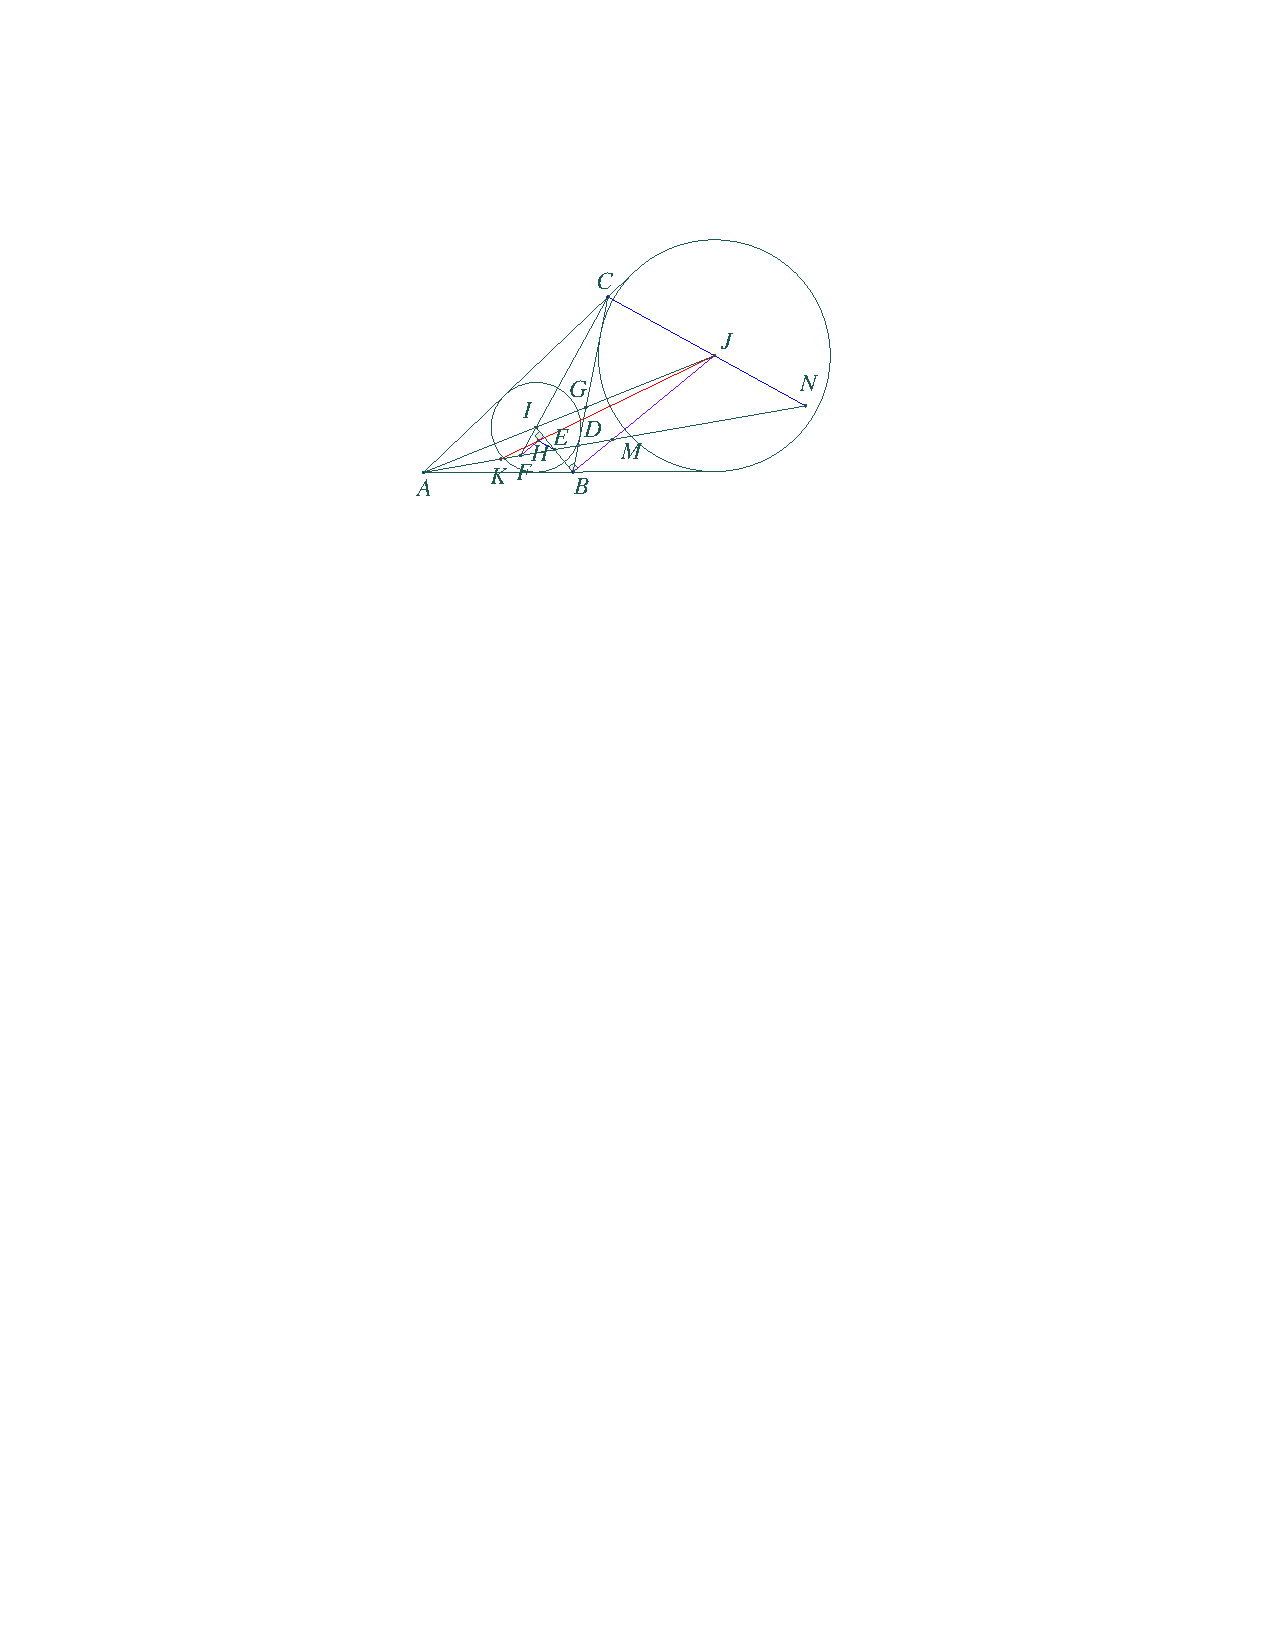
\includegraphics[width= 0.98\linewidth]{P738}
%		\caption{\small\textit{\color{}}}
		\vspace*{-20pt}
	\end{figure}
	Do $I$ là tâm đường tròn nội tiếp và $J$  là tâm đường tròn bàng tiếp góc $A$ của tam giác $ABC$, nên $BI$, $BJ$ tương ứng là phân giác trong, phân giác ngoài của góc $ABG$. Do đó, $IB \bot BJ$, và  $\left( {AGIJ} \right) =  - 1.$ Từ đây, do phép chiếu xuyên tâm bảo toàn tỷ số kép, nên
	\begin{align*}
		(ADEM) = B(ADEM) = B(AGIJ)= -1.
	\end{align*}
	Vì thế, do $K$ là trung điểm của $AD$, nên theo hệ thức Newton, ta có:
	\begin{align*}
		K{D^2} = \overline {KE}  \cdot \overline {KM} . \tag{$1$}
	\end{align*}
	Bằng cách tương tự, ta cũng chứng minh được
	\begin{align*}
		K{D^2} = \overline {KF}  \cdot \overline {KN} . \tag{$2$}
	\end{align*}
	Từ ($1$) và ($2$), suy ra
	\begin{align*}
		\overline {KE}  \cdot \overline {KM}  = \overline {KF}  \cdot \overline {KN} ;
	\end{align*}
	do đó, $\dfrac{{\overline {KE} }}{{\overline {KN} }} = \dfrac{{\overline {KF} }}{{\overline {KM} }}.$ \hfill ($3$)
	\vskip 0.05cm
	Đặt $\dfrac{{\overline {KE} }}{{\overline {KN} }} = k$;  và ký hiệu $f$ là phép vị tự tâm $K$, tỷ số $k$.
	\vskip 0.05cm
	Từ ($3$) suy ra, $f$ biến điểm $N$ thành điểm $E$, và biến điểm $M$ thành điểm $F$. \hfill ($4$)
	\vskip 0.05cm
	Tiếp theo, do $H$ là trực tâm tam giác $IEF$ (giả thiết) nên $FH \bot IE$, hay $FH \bot IB$ (do $I$, $E$, $B$ thẳng hàng). Mà $BJ \bot IB$ (chứng minh trên), hay $MJ \bot IB$ (do $M, B, J$ thẳng hàng), nên $FH \parallel MJ$.   \hfill     ($5$)
	\vskip 0.05cm
	Bằng cách hoàn toàn tương tự, ta cũng chứng minh được $EH \parallel NJ$.  \hfill   ($6$)
	\vskip 0.05cm
	Từ ($4$), ($5$) và ($6$) suy ra, $f$ biến đường thẳng $MJ$ thành đường thẳng $FH$, và biến đường thẳng $NJ$ thành đường thẳng $EH$. Do đó, $f$ biến điểm $J$ thành điểm $H$. Mà $K$ là tâm của $f$, nên $K, J, H$ thẳng hàng. Ta có điều phải chứng minh theo yêu cầu đề bài.
	\vskip 0.05cm
	\textbf{\color{thachthuctoanhoc}Bình luận và Nhận xét}
	\vskip 0.05cm
	$\pmb{1.}$ Lời giải trên cho thấy, kết luận của bài ra vẫn đúng, khi thay giả thiết ``$D$ thuộc cạnh $BC$, sao cho $A$, $I$, $D$ không thẳng hàng" bởi giả thiết ``$D$ thuộc đường thẳng $BC$, sao cho $A$, $I$, $D$ không thẳng hàng".
	\vskip 0.05cm
	$\pmb{2.}$ Tất cả các lời giải Tạp chí nhận được từ bạn đọc là lời giải đúng.
	\begin{flushright}
		\textbf{\color{thachthuctoanhoc}Hạ Vũ Anh}
	\end{flushright}
	{\color{thachthuctoanhoc}{\usefont{T5}{qag}{b}{n} P739.}}
	(Mức $A$) Cho dãy số $\left(a_n\right)$  xác định bởi
	\begin{align*}
		{a_n} = \left\lfloor {\frac{n}{{\sqrt 2 }}} \right\rfloor  + \left\lfloor {\frac{n}{{\sqrt 3 }}} \right\rfloor , \text{ với mọi } n \in \mathbb{N^*}.
	\end{align*}
	Chứng minh rằng, trong dãy $\left(a_n\right)$  có vô hạn số chẵn và vô hạn số lẻ.
	\vskip 0.1cm
	($\left\lfloor x \right\rfloor $  ký hiệu số nguyên lớn nhất không vượt quá $x$.)
	\vskip 0.05cm
	\textbf{\color{thachthuctoanhoc}Lời giải} (\textit{dựa trên ý tưởng của bạn Huỳnh Nguyễn Khánh Duy, lớp $12$ Toán, trường THPT chuyên Tiền Giang, tỉnh Tiền Giang})\textbf{\color{thachthuctoanhoc}.}
	\vskip 0.05cm
	Ta có Nhận xét sau:
	\vskip 0.05cm
	\textit{Nhận xét.} Với mọi  $x,y \in \mathbb{R}$, do 
	\begin{align*}
		x - 1 < \left\lfloor x \right\rfloor  \le x  \text{ và } y - 1 < \left\lfloor y \right\rfloor  \le y,
	\end{align*}
	nên
	\begin{align*}
		x - y - 1 < \left\lfloor x \right\rfloor  - \left\lfloor y \right\rfloor  < x - y + 1.
	\end{align*}
	Với mỗi $n \in \mathbb{N^*}$,  đặt
	\begin{align*}
		&{u_n} = \left\lfloor {\frac{{n + 1}}{{\sqrt 2 }}} \right\rfloor  - \left\lfloor {\frac{n}{{\sqrt 2 }}} \right\rfloor \\
		\text{ và } &{v_n} = \left\lfloor {\frac{{n + 1}}{{\sqrt 3 }}} \right\rfloor  - \left\lfloor {\frac{n}{{\sqrt 3 }}} \right\rfloor .
	\end{align*}  
	Theo Nhận xét, với mọi $n \in \mathbb{N^*}$, ta có:
	\begin{align*}
		&- 1 + \frac{1}{{\sqrt 2 }} = \frac{{n + 1}}{{\sqrt 2 }} - \frac{n}{{\sqrt 2 }} - 1 \\
		<\, &{u_n} < \frac{{n + 1}}{{\sqrt 2 }} - \frac{n}{{\sqrt 2 }} + 1 = 1 + \frac{1}{{\sqrt 2 }};
	\end{align*}
	mà $u_n \in \mathbb{Z}$  nên
	\begin{align*}
		u_n \in \{0;1\}  \text{ với mọi } n \in \mathbb{N^*}. \tag{$1$}
	\end{align*}
	Bằng cách hoàn toàn tương tự, ta cũng chứng minh được: 
	\begin{align*}
		v_n \in \{0;1\},  \text{ với mọi } n \in \mathbb{N^*}. \tag{$2$}
	\end{align*}
	Xét số nguyên dương $k$ tùy ý.
	\vskip 0.05cm
	Theo Nhận xét, ta có:
	\begin{align*}
		\sum\limits_{i = k}^{k + 100} {{u_i}}  &= \sum\limits_{i = k}^{k + 100} {\left( {\left\lfloor {\frac{{i + 1}}{{\sqrt 2 }}} \right\rfloor  - \left\lfloor {\frac{i}{{\sqrt 2 }}} \right\rfloor } \right)}  \\
		&= \left\lfloor {\frac{{k + 101}}{{\sqrt 2 }}} \right\rfloor  - \left\lfloor {\frac{k}{{\sqrt 2 }}} \right\rfloor  \\
		&> \frac{{k + 101}}{{\sqrt 2 }} - \frac{k}{{\sqrt 2 }} - 1 = \frac{{101}}{{\sqrt 2 }} - 1 \\
		&> 70, \tag{$3$}\\
		\sum\limits_{i = k}^{k + 100} {{v_i}}  &= \sum\limits_{i = k}^{k + 100} {\left( {\left\lfloor {\frac{{i + 1}}{{\sqrt 3 }}} \right\rfloor  - \left\lfloor {\frac{i}{{\sqrt 3 }}} \right\rfloor } \right)}  \\
		&= \left\lfloor {\frac{{k + 101}}{{\sqrt 3 }}} \right\rfloor  - \left\lfloor {\frac{k}{{\sqrt 3 }}} \right\rfloor \\
		& < \frac{{k + 101}}{{\sqrt 3 }} - \frac{k}{{\sqrt 3 }} + 1 = \frac{{101}}{{\sqrt 3 }} + 1\\
		& < 60. \tag{$4$}
	\end{align*}
	\vskip 0.1cm
	\columnbreak
	Từ ($1$) và ($3$) suy ra, trong $101$ số ${u_k},{u_{k \!+\! 1}},\! \ldots \!,{u_{k \!+\! 100}}$ có ít nhất $71$ số bằng $1$.
	\vskip 0.05cm
	Từ ($2$) và ($4$) suy ra, trong $101$ số ${v_k},{v_{k + 1}}, \ldots ,{v_{k + 100}}$  có tối đa $59$ số bằng $1$.
	\vskip 0.05cm
	Vì vậy, tồn tại $m \in \{k; k + 1; \ldots; k + 100\}$ sao cho $u_m = 1$  và $v_m = 0$.
	\vskip 0.05cm 
	Ta có:
	\begin{align*}
		&{a_{m + 1}} - {a_m}\\
		= &\left\lfloor {\frac{{m + 1}}{{\sqrt 2 }}} \right\rfloor  + \left\lfloor {\frac{{m + 1}}{{\sqrt 3 }}} \right\rfloor  - \left\lfloor {\frac{m}{{\sqrt 2 }}} \right\rfloor  - \left\lfloor {\frac{m}{{\sqrt 3 }}} \right\rfloor  \\
		= \,\,&{u_m} + {v_m} = 1.
	\end{align*}
	Suy ra, ${a_m}\not  \equiv {a_{m + 1}}\left( {\bmod 2} \right).$  Từ đây, do tính tùy ý của số nguyên dương $k$, suy ra, trong $101$ số hạng liên tiếp tùy ý của dãy $\left(a_n\right)$  luôn có đồng thời cả số chẵn và số lẻ. Mà $\left(a_n\right)$  là dãy vô hạn, nên trong dãy đó có vô hạn số chẵn và vô hạn số lẻ. Ta có điều phải chứng minh theo yêu cầu đề bài.
	\vskip 0.05cm
	\textbf{\color{thachthuctoanhoc}Bình luận và Nhận xét}
	\vskip 0.05cm
	Lời giải của bạn \textit{Huỳnh Nguyễn Khánh Duy} là lời giải duy nhất Tạp chí nhận được từ bạn đọc, và là một lời giải đúng.
	\begin{flushright}
		\textbf{\color{thachthuctoanhoc}Lưu Thị Thanh Hà}
	\end{flushright}
	{\color{thachthuctoanhoc}{\usefont{T5}{qag}{b}{n} P740.}}
	(Mức $A$) Cho bảng ô vuông kích thước $2023 \times 2023$. Tìm số nguyên dương $n$ nhỏ nhất, sao cho có thể đặt $n$ viên bi vào các ô vuông con của bảng, đảm bảo các điều kiện sau được đồng thời thỏa mãn:
	\vskip 0.05cm
	$i/$ Ở mỗi ô vuông con chỉ có tối đa một viên bi;
	\vskip 0.05cm
	$ii/$ Với mỗi ô vuông con không có bi, tổng số viên bi ở hàng và cột chứa ô đó không nhỏ hơn $2023$.
	\vskip 0.05cm
	\textbf{\color{thachthuctoanhoc}Lời giải} (\textit{dựa theo cách giải của bạn Nguyễn Gia Khánh, lớp $12$ Toán $1$, trường THPT chuyên Hưng Yên, tỉnh Hưng Yên})\textbf{\color{thachthuctoanhoc}.}
	\vskip 0.05cm
	Đánh số thứ tự các hàng của bảng đã cho, từ trên xuống dưới, lần lượt bởi $1, 2, \ldots, 2023$; và đánh số thứ tự các cột của bảng đó, từ trái qua phải, lần lượt bởi $1, 2, \ldots, 2023$.
	\vskip 0.05cm
	Với mỗi $i \in  \{1; 2; \ldots; 2023\}$, ta gọi hàng được đánh số thứ tự $i$ là hàng $i$, và gọi cột được đánh số thứ tự $i$ là cột $i$.
	\vskip 0.05cm
	Với $i, j \in \{1; 2; \ldots; 2023\}$, ký hiệu ô vuông con nằm ở giao của hàng thứ $i$ và cột thứ $j$ bởi $(i, j)$.
	\vskip 0.05cm
	Giả sử $n$ là số nguyên dương sao cho có thể đặt $n$ viên bi vào các ô vuông con của bảng, đảm bảo các điều kiện $i/$ và $ii/$ được đồng thời thỏa mãn.
	\vskip 0.05cm
	Xét một cách đặt bi tùy ý, thỏa mãn các yêu cầu của đề bài.
	\vskip 0.05cm
	Với mỗi $i \in \{1; 2; \ldots; 2023\}$, gọi $a_i$  là số viên bi được đặt vào hàng $i$, và  $b_i$ là số viên bi được đặt vào cột $i$.
	\vskip 0.05cm
	Do tổng số viên bi được đặt vào bảng bằng $n$, nên
	\begin{align*}
		\sum\limits_{i = 1}^{2023} {{a_i}}  = \sum\limits_{i = 1}^{2023} {{b_i}}  = n. \tag{$1$}
	\end{align*}
	Đặt $m = 2023^2 -n$. \hfill    ($2$)
	\vskip 0.05cm
	Do số bi ở mỗi ô tối đa là $1$ và trong bảng có $n$ viên bi, nên trong bảng có đúng $n$ ô có bi. Vì thế, trong bảng có đúng $m$ ô không có bi. Giả sử các ô này là $(p_1,q_1), (p_2,q_2), \ldots, (p_m,q_m)$.
	\vskip 0.05cm 
	Theo giả thiết của bài ra, với mọi\linebreak $i \in \{1; 2; \ldots; m\}$, đều có
	\begin{align*}
		{a_{{p_i}}} + {b_{{q_i}}} \ge 2023. \tag{$3$}
	\end{align*}
	Với mỗi $k \in \{1; 2; \ldots; 2023\}$, do trong hàng $k$ có đúng $2023 - a_k$  ô không có bi, và trong cột $k$ có đúng $2023-b_k$  ô không có bi, nên số $k$ xuất hiện đúng $2023- a_k$  lần trong dãy $p_1,p_2,\ldots,p_m$  và xuất hiện đúng $2023-b_k$  lần trong dãy $q_1, q_2,\ldots,q_m$.
	\vskip 0.05cm 
	Vì vậy
	\begin{align*}
		\sum\limits_{i = 1}^m {{a_{{p_i}}}} & = \sum\limits_{k = 1}^{2023} {\left( {2023 - {a_k}} \right){a_k}} \\
		& = 2023 \cdot \sum\limits_{k = 1}^{2023} {{a_k}}  - \sum\limits_{k = 1}^{2023} {a_k^2}  \\
		&= 2023 \cdot n - \sum\limits_{k = 1}^{2023} {a_k^2} \quad\text{(do ($1$))}; \tag{$4$}\\
		\sum\limits_{i = 1}^m {{b_{{q_i}}}}  &= \sum\limits_{k = 1}^{2023} {\left( {2023 - {b_k}} \right){b_k}}  \\
		&= 2023 \cdot \sum\limits_{k = 1}^{2023} {{b_k}}  - \sum\limits_{k = 1}^{2023} {b_k^2}  \\
		&= 2023 \cdot n - \sum\limits_{k = 1}^{2023} {b_k^2} \quad\text{(do ($1$))}. \tag{$5$}
	\end{align*}
	Từ ($3$), ($4$) và ($5$), với lưu ý tới ($2$), suy ra
	\begin{align*}
		&2023\left( {{{2023}^2} - n} \right) \le \sum\limits_{i = 1}^m {\left( {{a_{{p_i}}} + {b_{{q_i}}}} \right)}  \\
		= \,&2 \cdot 2023n - \sum\limits_{k = 1}^{2023} {\left( {a_k^2 + b_k^2} \right)} .
	\end{align*}
	Do đó
	\begin{align*}
			3 \cdot 2023n &\ge {2023^3} + \sum\limits_{k = 1}^{2023} {\left( {a_k^2 + b_k^2} \right)}  \\
			&\ge {2023^3} + \sum\limits_{k = 1}^{2023} {\frac{{{{\left( {{a_k} + {b_k}} \right)}^2}}}{2}} \\
			 &\ge {2023^3} + \frac{{{{\left( {\sum\limits_{k = 1}^{2023} {\left( {{a_k} + {b_k}} \right)} } \right)}^2}}}{{2 \cdot 2023}} \\
			 &= {2023^3} + \frac{{{{\left( {2n} \right)}^2}}}{{2 \cdot 2023}} \quad\left( {{\rm{do}}(1)} \right).
	\end{align*}
	Suy ra
	\begin{align*}
		2{n^2} - 3 \cdot {2023^2} \cdot n + {2023^4} \le 0.
	\end{align*}
	Vì vậy
	\begin{align*}
		n \ge \frac{{{{2023}^2}}}{2} &= \frac{{2\left( {{{1011}^2} + {{1012}^2}} \right) - 1}}{2} \\
		&= {1011^2} + {1012^2} - \frac{1}{2}.
	\end{align*}
	Từ đó, do $n \in \mathbb{N^*}$,  suy ra  $n \ge {1011^2} + {1012^2}$.
	\vskip 0.05cm
	Xét cách đặt $1011^2 + 1012^2$  viên bi vào bảng, như sau:
	\vskip 0.05cm
	Đặt vào mỗi ô vuông con của bảng con $1011 \times 1011$, tạo bởi các hàng $1, 2, \ldots, 1011$ và các cột $1, 2, \ldots, 1011$, một viên bi; và đặt vào mỗi ô vuông con của bảng con $1012 \times 1012$, tạo bởi các hàng $1012, 1013, \ldots, 2023$ và các cột $1012, 1013, \ldots, 2023$, một viên bi.
	\vskip 0.05cm
	Dễ thấy, ở cách đặt trên, với mỗi ô vuông con không có bi, tổng số viên bi ở hàng và cột chứa ô đó đúng bằng $2023$. Vì thế, cách đặt đó thỏa mãn tất cả các điều kiện của đề bài.
	\vskip 0.05cm
	Vì vậy, $n = 1011^2 + 1012^2$ là số nguyên dương nhỏ nhất thỏa mãn yêu cầu đề bài.
	\vskip 0.05cm
	\textbf{\color{thachthuctoanhoc}Bình luận và Nhận xét}
	\vskip 0.05cm
	$\pmb{1.}$ Có thể phát biểu bài đã ra một cách đơn giản hơn, như sau:
	\vskip 0.05cm
	``Cho bảng ô vuông kích thước $2023 \times 2023$. Tìm số nguyên dương $n$ nhỏ nhất, để có thể đánh dấu $n$ ô vuông con của bảng, sao cho với mỗi ô vuông con không được đánh dấu, tổng số ô được đánh dấu ở hàng và cột chứa ô đó không nhỏ hơn $2023$."
	\vskip 0.05cm
	$\pmb{2.}$ Trong số các lời giải Tạp chí nhận được từ bạn đọc, lời giải của bạn \textit{Nguyễn Gia Khánh} là lời giải đúng duy nhất; các lời giải còn lại đều mắc lỗi thiếu kiểm tra cách đặt $1011^2 + 1012^2$ viên bi, đã chỉ ra ở lời giải, có thỏa mãn các điều kiện của đề bài hay không.
	\begin{flushright}
		\textbf{\color{thachthuctoanhoc}Nguyễn Khắc Minh}
	\end{flushright}
\end{multicols}
\newpage
\begin{center}
	\textbf{\color{thachthuctoanhoc}DANH SÁCH HỌC SINH CÓ LỜI GIẢI ĐÚNG}
\end{center}
\textit{Trong các ngoặc đơn ở phần dưới đây, sau tên lớp là mã hiệu của các bài toán mà học sinh có lời giải đúng.}
\begin{multicols}{2}
	\textbf{\color{thachthuctoanhoc}KHỐI THCS}
	\vskip 0.05cm
	$\bullet$ Trường \textbf{\color{thachthuctoanhoc}THCS Nguyễn Thái Bình}, tỉnh Cà Mau: \textit{Lê Nguyễn Hoàng Nhật Đình} (lớp $9$C; P$731$, P$732$, P$733$, P$734$, P$736$, P$737$).
	\vskip 0.05cm
	$\bullet$ Trường \textbf{\color{thachthuctoanhoc}TH\&THCS Archimedes Đông Anh}, Tp. Hà Nội: \textit{Ngô Minh Chấn} (lớp $9$A$3$; P$732$, P$733$, P$735$).
	\vskip 0.05cm
	$\bullet$ Trường \textbf{\color{thachthuctoanhoc}THCS Thanh Xuân}, Quận Thanh Xuân, Tp. Hà Nội: \textit{Doãn Hải Dương} (lớp $7$A$6$; P$735$).
	\vskip 0.05cm
	$\bullet$ Trường \textbf{\color{thachthuctoanhoc}THCS Nguyễn Tri Phương}, Tp. Huế, tỉnh Thừa Thiên -- Huế: \textit{Lê Trung Tấn Huy} (lớp $9/6$; P$733$, P$734$, P$735$, P$737$).
	\vskip 0.05cm
	$\bullet$ Trường \textbf{\color{thachthuctoanhoc}THCS Nguyễn Chí Thanh}, tỉnh Phú Yên: \textit{Nguyễn Nguyên Chinh} (lớp $9$D; P$734$).
	\vskip 0.05cm
	\textbf{\color{thachthuctoanhoc}KHỐI THPT}
	\vskip 0.05cm
	$\bullet$ Trường \textbf{\color{thachthuctoanhoc}THPT chuyên Lê Quý Đôn}, tỉnh Điện Biên: \textit{Nguyễn Ngọc Diệp} (lớp $10$A$1$; P$731$).
	\vskip 0.05cm
	$\bullet$ Trường \textbf{\color{thachthuctoanhoc}THPT chuyên Nguyễn Quang Diêu}, tỉnh Đồng Tháp: \textit{Đỗ Duy Quang} (lớp $12$T$1$; P$731$, P$734$, P$737$), \textit{Lâm Nhật Tiến} (lớp $12$T$1$; P$734$).
	\vskip 0.05cm
	$\bullet$ Trường \textbf{\color{thachthuctoanhoc}THPT Hà Đông}, tỉnh Hải Dương: \textit{Phạm Văn Đăng} (lớp $11$A; P$735$).
	\vskip 0.05cm
	$\bullet$ Trường \textbf{\color{thachthuctoanhoc}THPT chuyên Hưng Yên}, tỉnh Hưng Yên: \textit{Phạm Thị Minh Ánh} (lớp $12$ Toán $1$; P$737$), \textit{Nguyễn Gia Khánh} (lớp $12$ Toán $1$; P$738$, P$740$).
	\vskip 0.05cm
	$\bullet$ Trường \textbf{\color{thachthuctoanhoc}THPT chuyên Lê Hồng Phong}, tỉnh Nam Định: \textit{Phạm Đức Minh} (lớp $10$ Toán $2$; P$731$, P$736$, P$737$).
	\vskip 0.05cm
	$\bullet$ Trường \textbf{\color{thachthuctoanhoc}THPT chuyên Lương Văn Chánh}, tỉnh Phú Yên: \textit{Đặng Kỳ Nam} (lớp $10$ Toán $1$; P$731$, P$734$).
	\vskip 0.05cm
	$\bullet$ Trường \textbf{\color{thachthuctoanhoc}THPT chuyên Võ Nguyên Giáp}, tỉnh Quảng Bình: \textit{Trần Đức Phát} (lớp $10$T$1$; P$735$).
	\vskip 0.05cm
	$\bullet$ Trường \textbf{\color{thachthuctoanhoc}THPT chuyên Tiền Giang}, tỉnh Tiền Giang: \textit{Huỳnh Nguyễn Khánh Duy} (lớp $12$ Toán; P$739$), \textit{Nguyễn Huy Hoàng} (lớp $11$ chuyên Toán; P$731$), \textit{Trương Phúc Vinh} (lớp $12$ Lý; P$731$).
	\vskip 0.05cm
	$\bullet$ Trường \textbf{\color{thachthuctoanhoc}THPT chuyên Thái Nguyên}, tỉnh Thái Nguyên: \textit{Nguyễn Tiến Dũng} (lớp $11$ Toán; P$735$).
	\vskip 0.05cm
	$\bullet$ Trường \textbf{\color{thachthuctoanhoc}THPT chuyên Vĩnh Phúc}, tỉnh Vĩnh Phúc: \textit{Trương Anh Dũng} (lớp $10$A$1$; P$731$, P$733$, P$737$).
\end{multicols}

%	\newpage 
%	
%	\setcounter{figure}{0}
%	\thispagestyle{cackithitoannone}
\pagestyle{cackithitoan}
\everymath{\color{cackithi}}
\graphicspath{{../cackithi/pic/}}
\blfootnote{\color{cackithi}$^1$Khoa Toán Đại học Osnabrueck, CHLB Đức.}
\begingroup
\AddToShipoutPicture*{\put(0,616){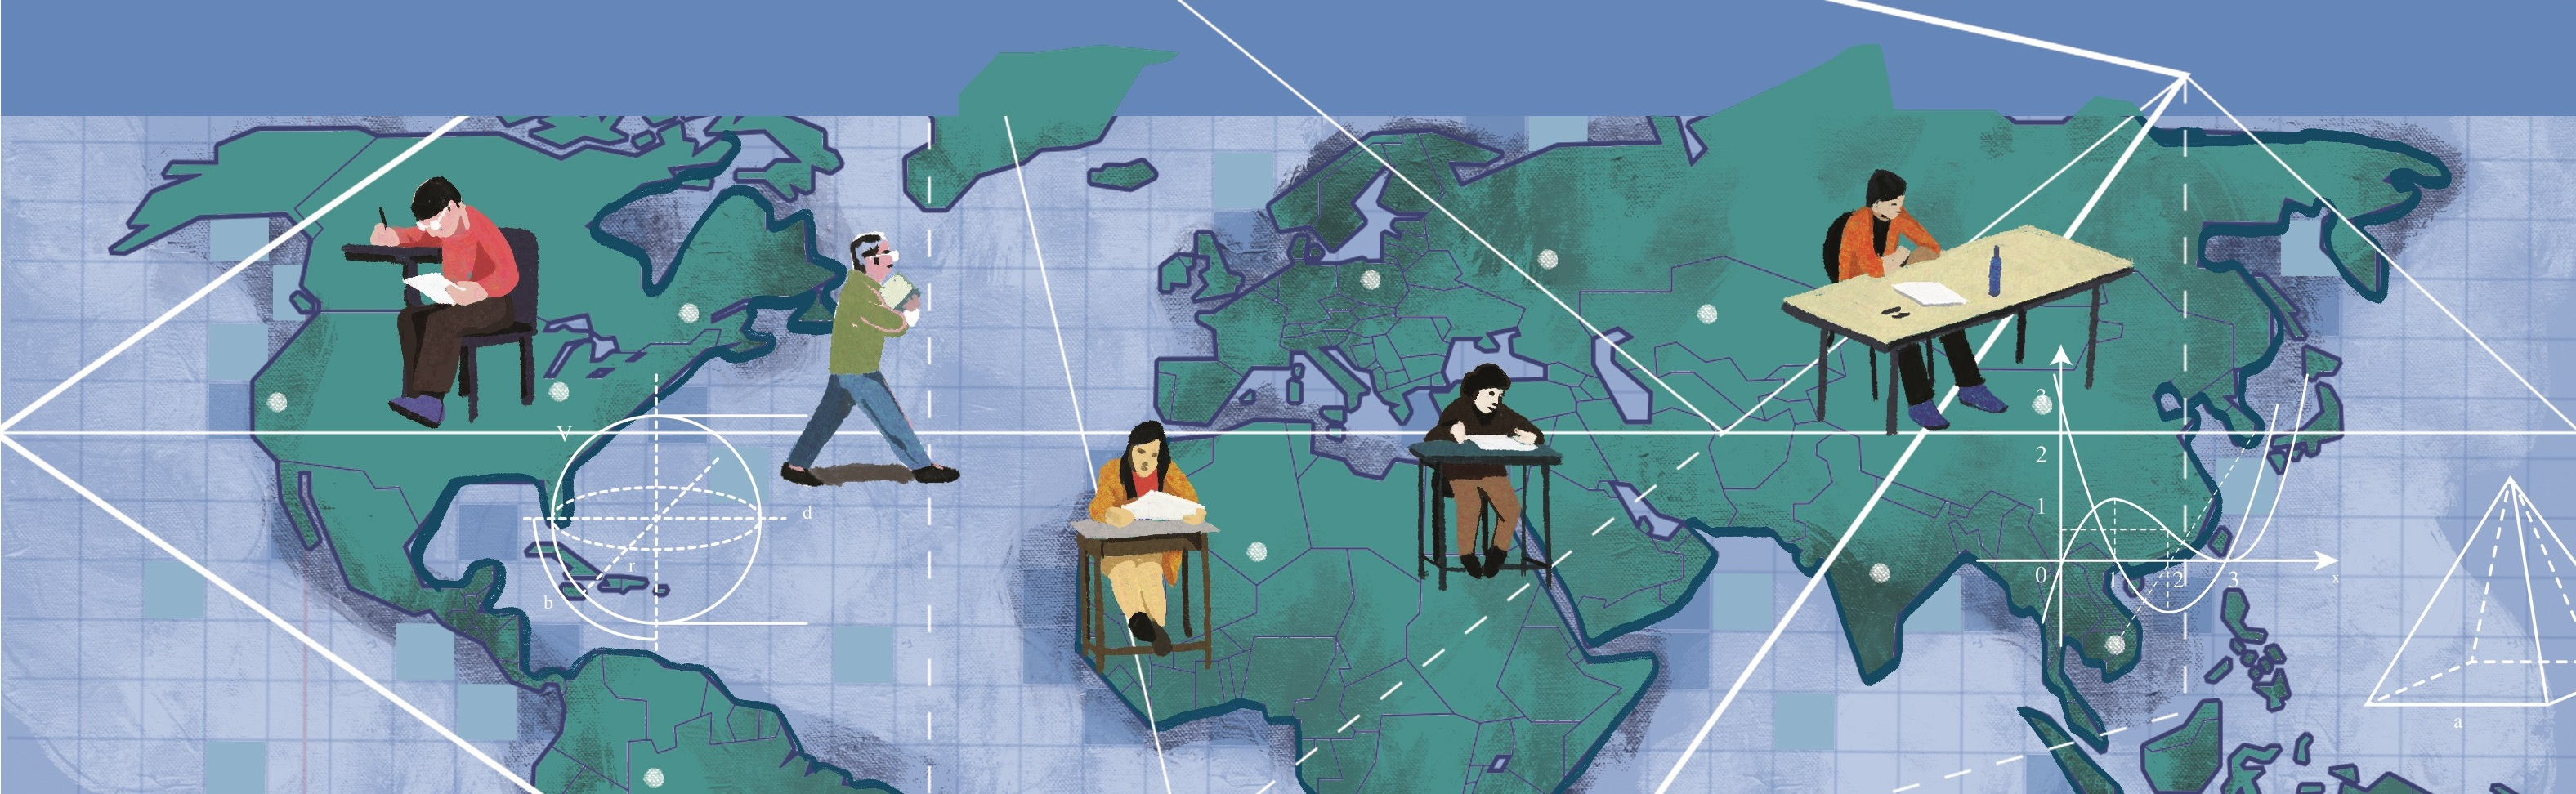
\includegraphics[width=19.3cm]{../bannercackithi}}}
\AddToShipoutPicture*{\put(82,527){
\includegraphics[scale=1]{../tieude2.pdf}}}
\centering
\endgroup
\vspace*{182pt}

\begin{multicols}{2}
	Trong chuyên mục này, chúng tôi sẽ trình bày Lời giải của các bài toán trong vòng hai kỳ thi toán học liên bang Đức năm $2023$, đăng trong số báo $9/2023$. 
	\vskip 0.1cm
	\textbf{\color{cackithi}Câu $\pmb{1}$:} Tìm ước chung lớn nhất của tất cả các số có dạng $p^6 - 7p^2 +6$ với $p$ chạy trên tập tất cả các số nguyên tố và $p \ge 11$.
	\vskip 0.1cm
	\textit{Lời giải.}
	Đặt $f(p) \colon =p^6 - 7p^2 +6$. Gọi $a$ là ước chung lớn nhất (ƯCLN) của tất cả các $f(p)$ với $p$ nguyên tố và $p \ge 11$. Ta sẽ chứng minh rằng $a = 2^5\times 3 \times 7$.
	\vskip 0.1cm	
	Thật vậy, theo định lý Fermat nhỏ thì $7|p^6 - 1$ với mọi số nguyên $7 \not | p$. Do đó, $7 |p^6 - 1  - 7p^2 + 7 = f(p)$ với mọi $p$ như trên và ta có $7 | a$.
	\vskip 0.1cm	
	Mặt khác, 
	$f(p) = (p^2-1)(p^2-2)(p^2+3) \equiv (p^2-1)(p^2-2)p^2 \mod 3 \equiv 0 \mod 3$ do $p^2, p^2-1, p^2-2$ là ba số nguyên liên tiếp. Như vậy, $3 | f(p)$ với mọi $p$ và ta thu được $3|a$.
	\vskip 0.1cm	
	Hơn nữa, do $p$ nguyên tố và $p \ge 11$ nên $p$ là số lẻ. Đặt $p= 2k+1$, ta có
	\begin{align*}
			f(p) = & (p^2-1)(p^2-2)(p^2+3) \\
			= & (4k^2 \!+\! 4k) \!(4k^2 \!+\! 4k\!-\!1)(4k^2\!+\!4k\!+\!4) \\
			= & 16k(k\!+\!1)(4k^2 \!+\! 4k\!-\!1)(k^2 \!+\! k \!+\! 1).
	\end{align*}
	Vì $2 |k(k+1)$ với mọi $k \in \mathbb{Z}$ nên $2\times 16 = 32 = 2^5 |f(p)$. Bởi vậy $2^5 |a$.
	\vskip 0.1cm
	Do $2^5, 3$ và $7$ đôi một nguyên tố cùng nhau nên
	\begin{align*}
		2^5 \times 3 \times 7 |a. \tag{$1$}
	\end{align*}
		Mặt khác, vì
		$
		f(11) = 1770720 = 2^5 \times 3 \times 5 \times 7 \times 17 \times 31
		$
		và
		$
		f(13) = 4825632 = 2^5 \times 3 \times 7 \times 43 \times 167
		$
		nên 
		\begin{align*}
			a |\text{ƯCLN}(f(11), f(13)) \!=\! 2^5\!\times\! 3 \!\times\! 7. \tag{$2$}
		\end{align*}
		Từ ($1$) và ($2$) ta thu được $a = 2^5\times 3 \times 7$.
	\vskip 0.1cm
	\textbf{\color{cackithi}Câu $\pmb{2}$:} Trên một hòn đảo địa hình đồi núi có $2023$ điểm quan sát. Từ mỗi điểm quan sát có thể nhìn thấy ít nhất $42$ điểm quan sát khác. Với hai điểm quan sát bất kỳ $X$ và $Y$, luôn tồn tại một số nguyên dương $n$ và các điểm quan sát $A_1,  A_2, \ldots, A_{n+1}$ sao cho $A_1 = X$, $A_{n+1} = Y$ và mỗi cặp điểm liền kề $A_i$ với $A_{i+1}$ có thể quan sát được lẫn nhau với $i = 1, 2, \ldots, n$. Số $n$ nhỏ nhất như vậy được gọi là khoảng cách quan sát (Sichtabstand). 
	\vskip 0.1cm
	Xác định khoảng cách quan sát lớn nhất có thể có giữa hai cặp điểm quan sát thỏa mãn những điều kiện ở trên.
	\vskip 0.1cm
	\textit{Lời giải.}
	Ta sẽ chứng minh rằng khoảng cách quan sát lớn nhất có thể là $140$.
	\vskip 0.1cm	
	Với hai điểm quan sát $X,Y$ trong bài, ta nói $A_1, \ldots, A_{n+1}$ là các điểm thuộc \textit{chuỗi quan sát} độ dài $n$ nối $X$ và $Y$. Để tìm một chuỗi quan sát có độ dài nhỏ nhất, ta chỉ cần xét trường hợp mỗi điểm quan sát trong chuỗi xuất hiện đúng một lần. Vì chỉ có hữu hạn điểm quan sát nên độ dài các chuỗi quan sát là hữu hạn (bị chặn trên bởi $2022$). Như vậy giữa tất cả các chuỗi quan sát nối $X$ và $Y$ luôn tồn tại chuỗi quan sát có độ dài ngắn nhất, và độ dài này chính là khoảng cách quan sát được định nghĩa ở trên. Do chỉ có hữu hạn các cặp điểm quan sát, tồn tại một cặp điểm có khoảng cách quan sát lớn nhất.
	\vskip 0.1cm	
	Cho trước một hệ thống tùy ý $M$ gồm $2023$ điểm quan sát thỏa mãn yêu cầu của bài toán. Chọn $X \in M$ bất kỳ và gọi $M_i$ tập các điểm quan sát có khoảng cách quan sát $i$ tới $X$. Ta cũng sẽ đặt $M_0 = \{X\}$. Do với bất kỳ $Y \in M$ luôn tồn tại một chuỗi quan sát nối $X$ và $Y$ nên các tập $M_i$ lập nên một phân hoạch của $M$. Nói cách khác, $M = \cup_{i}M_i$ và $M_i \cap M_j = \emptyset$ nếu $i\neq j$.
	\vskip 0.1cm
	Gọi $n(X)$ là chỉ số sao cho $M_{n(X)} \neq \emptyset$ và $M_i = \emptyset$ với mọi $i \ge n(X)$. Bằng định nghĩa, với mỗi $Y \in M_{n(X)}$ luôn tồn tại chuỗi quan sát ngắn nhất $A_1, \ldots A_{n(X) + 1}$ với $A_1 = X$ và $A_{n(X)+1} = Y$. Rõ ràng $A_i, A_{i+1}, \ldots, A_{j}$ cũng là chuỗi quan sát ngắn nhất giữa $A_i$ và $A_j$ với mọi $1 \le i <j \le n(X) + 1$. Nói riêng, $A_i \in M_{i-1}$ và ta có $M_i \neq \emptyset$ với mọi $i \le n(X)$.
	\vskip 0.1cm	
	Hơn nữa, từ mỗi điểm trong $M_i$ chỉ có thể quan sát được các điểm trong $M_{i-1}, M_i$ và $M_{i+1}$. Thật vậy, nếu từ $V \in M_i$ quan sát được $W \in M_j$ với $j \le i-2$ thì $V \in M_{j+1}$. Do đó, $V \in M_i \cap M_{j+1}$. Điều này vô lý vì $M_i \cap M_{j+1} = \emptyset$ do $j+1 \neq i$. Tương tự, từ $V \in M_i$ quan sát được $W \in M_j$ với $j \ge i+2$ cũng dẫn đến mâu thuẫn. Vì từ mỗi $V \in M_i$ có thể quan sát được ít nhất $42$ điểm khác và các điểm này nằm trong $M_{i-1}, M_i, M_{i+1}$ nên
	\begin{align*}
		|M_{i-1} \cup M_i \cup M_{i+1}| \ge 43.
	\end{align*}
	Từ $X \in M_0$ chỉ quan sát được các điểm trong $M_1$ và từ $Y \in M_{n(X)}$ chỉ quan sát được các điểm từ $M_{n(X)}$ và $M_{n(X)-1}$ nên
	\begin{align*}
		|M_0 \cup M_1| \ge 43 \text{ và } |M_{n(X)-1} \cup M_{n(X)}| \ge 43.
	\end{align*}
	\textbf{\color{cackithi}Khẳng định $\pmb{1}$:} \textit{Khoảng cách quan sát lớn nhất không thể lớn hơn $140$.} 
	\vskip 0.1cm
	Thật vậy, nếu $M_{141} \neq \emptyset$ thì 
	\begin{align*}
		& |M_0 \cup M_1| + |M_2 \cup M_3 \cup M_4| \\
		&+ |M_5 \cup M_6 \cup M7| + \ldots \\
		&+ |M_{137} \cup M_{138} \cup M_{139}| + |M_{140} \cup M_{141}| \\
		\ge \,&43 + 46.43 + 43 = 2064 > 2023
	\end{align*}
	dẫn đến mâu thuẫn.
	\vskip 0.1cm
		\textbf{\color{cackithi}Khẳng định $\pmb{2}$:} \textit{Tồn tại một hệ thống điểm quan sát sao cho khoảng cách quan sát lớn nhất là $140$.} 
		\vskip 0.1cm
		Thật vậy, xây dựng $141$ tập không rỗng $M_i$ với $i = 0, \ldots, 140$ như trong Hình $1$, trong đó:
		\vskip 0.1cm
		\begin{figure}[H]
				\vspace*{-5pt}
				\centering
				\captionsetup{labelformat= empty, justification=centering}
			\resizebox{\columnwidth}{!}{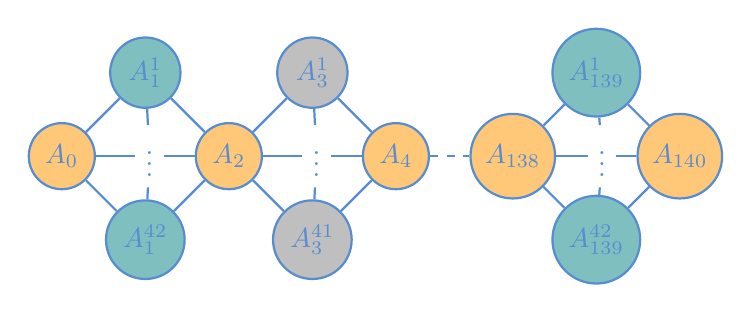
\begin{tikzpicture}[node distance={15mm}, thick, main/.style = {draw, circle}, cackithi] 
				\node[main, fill={rgb:orange,1;yellow,2;pink,5}] (1) {$A_0$}; 
				\node[main, fill= teal!50] (2) [above right of=1] {$A_1^1$}; 
				\node (3) [right = 5mm of 1] {$\vdots$};
				
				\node[main, fill= teal!50] (4) [below right of=1] {$A_1^{42}$}; 
				\node[main, fill={rgb:orange,1;yellow,2;pink,5}] (5) [below right of=2] {$A_2$}; 
				\node[main,fill=gray!50] (6) [above right of=5] {$A_3^1$}; 
				\node (7) [right = 5mm of 5] {$\vdots$};
				\node[main, fill=gray!50] (8) [below right of=5] {$A_3^{41}$}; 
				\draw (1) -- (2); 
				\draw (1) -- (3); 
				\draw (1) -- (4); 
				\draw (2) -- (3);
				\draw (3) -- (4);
				\draw (2) -- (5); 
				\draw (3) -- (5); 
				\draw (4) -- (5); 
				\draw (5) -- (6);
				\draw (5) -- (7);
				\draw (5) -- (8);   
				\draw (6) -- (7);
				\draw (7) -- (8);
				\node[main, fill={rgb:orange,1;yellow,2;pink,5}] (9) [below right of=6] {$A_4$};
				\draw (6) -- (9);
				\draw (7) -- (9); 
				\draw (8) -- (9);  
				\node[main, fill={rgb:orange,1;yellow,2;pink,5}] (10) [right = 5mm of 9] {$A_{138}$};
				\draw[dashed] (9) -- (10);  
				\node[main, fill= teal!50] (11) [above right of=10] {$A_{139}^1$}; 
				\node (12) [right = 4mm of 10] {$\vdots$}; 
				\node[main, fill= teal!50] (13) [below right of=10] {$A_{139}^{42}$}; 
				\draw (10) -- (11);
				\draw (10) -- (12);
				\draw (10) -- (13);
				\draw (11) -- (12);
				\draw (12) -- (13);
				\node[main, fill={rgb:orange,1;yellow,2;pink,5}] (14) [below right of=11] {$A_{140}$};
				\draw (11) -- (14);
				\draw (12) -- (14);
				\draw (13) -- (14);
			\end{tikzpicture}}
			\caption{\small\textit{\color{cackithi}Hình $1$. Hệ thống điểm quan sát với khoảng cách quan sát lớn nhất $140$. Mỗi điểm $A_i^{\bullet}$ thuộc tập $M_i$ có thể quan sát được tất cả điểm trong $M_{i-1}, M_{i+1}$ cũng như các điểm còn lại trong $M_i$.}}
			\vspace*{-10pt}
		\end{figure}
		\vskip 0.1cm		
		$\bullet$ Mỗi tập $M_{3k}$ và $M_{3k+2}$ với $k = 0, \ldots, 46$ chỉ chứa một điểm quan sát.
		\vskip 0.1cm
		$\bullet$ Mỗi tập $M_{1}$ và $M_{139}$ có $42$ điểm quan sát.
		\vskip 0.1cm
		$\bullet$ Mỗi tập $M_{3k+1}$ với $k = 1, \ldots, 45$ có $41$ điểm quan sát.
		\vskip 0.1cm
		Độc giả có thể kiểm tra rằng hệ thống này có $2023$ điểm quan sát và thỏa mãn điều kiện của bài toán. Ở đó, điểm quan sát duy nhất trong $M_{140}$ có khoảng cách quan sát $140$ tới điểm quan sát duy nhất trong $M_0$.
		\vskip 0.1cm
	\textbf{\color{cackithi}Câu $\pmb{3}$:} Cho tam giác $ABC$ với tâm đường tròn nội tiếp $I$. Gọi trung điểm của các cạnh $AC$ và $BC$ lần lượt là $M_b$ và $M_a$. Gọi giao điểm của đường thẳng $M_bI$ với đường thẳng $BC$ là $B'$ và giao điểm của đường thẳng $M_aI$ với đường thẳng $AC$ là $A'$. Biết rằng hai tam giác $ABC$ và $A'B'C$ có cùng diện tích. 
	\vskip 0.1cm
	Tìm giá trị có thể của góc $ACB$.\footnote{\color{cackithi}Trong số $09/2023$ chúng tôi đã sai sót khi yêu cầu tìm giá trị \textbf{\color{cackithi}lớn nhất} có thể của góc $ACB$. Thành thật xin lỗi các độc giả của Pi.}	
		\begin{figure}[H]
			\vspace*{-10pt}
			\centering
			\captionsetup{labelformat= empty, justification=centering}
			\resizebox{\columnwidth}{!}{\begin{tikzpicture}
				\tkzSetUpPoint[size=4,circle, fill= teal!50]
				\tkzDefPoints{0/0/A,6/0/B,0.8/4/C}
				
				\tkzDefTriangleCenter[centroid](A,B,C)
				\tkzGetPoint{G}
				\tkzDefSpcTriangle[medial](A,B,C){Ma,Mb,Mc}
				%\tkzLabelPoints(A,B,C)
				\tkzDefTriangleCenter[in](A,B,C)
				\tkzGetPoint{I}
				
				\tkzDefCircle[in](A,B,C) 
				\tkzGetPoints{I}{i}
				
				\tkzInterLL(Mb,I)(B,C)
				\tkzGetPoint{B1}
				\tkzInterLL(Ma,I)(A,C)
				\tkzGetPoint{A1}
				\tkzDrawSegments(A,B B,C C,A)
				\tkzDrawPoints(A1,B1)
				\tkzLabelPoint[above left](A1){$A'$}
				\tkzLabelPoint(B1){$B'$}
				\tkzDrawLines[dashed](B1,Mb A1,Ma)
				\tkzDrawSegments(B1,B A1,B1)
				\tkzDrawCircle(I,i)
				\tkzDrawPoints(I, Mb, Ma)
				
				\tkzDrawPoints(A,B,C)
				
				\tkzLabelPoint(I){$I$}
				
				\tkzLabelPoints[below left](A,Mb)
				\tkzLabelPoints[above right](B,Ma)
				\tkzLabelPoint[above](C){$C$}
			\end{tikzpicture}}
		\vspace*{-10pt}
		\end{figure}
		\textit{Lời giải.} Gọi độ dài các cạnh $AB$, $BC$ và $CA$ lần lượt là $c$, $a$, $b$. Đặt $\gamma \colon = \angle ACB$. Ta sẽ chứng minh rằng $\gamma = 60^{\circ}$.
		\vskip 0.1cm
		Thật vậy, từ $M_a$ vẽ đường thẳng song song với $AC$ và cắt $CI$ tại $P$. Vì $\angle CPM_a = \angle A'CI = \gamma/2$ nên tam giác $CM_aP$ cân tại $M_a$ và ta có $M_aP = M_aC = a/2 = M_aB$. Như vậy $P$ nằm trên đường tròn tâm $M_a$ bán kính $a/2$. Từ đó suy ra tam giác $BPC$ vuông tại $P$ và ta thu được 
		\begin{align*}
			CP = CB \cos (\gamma /2) = a \cos(\gamma/2).
		\end{align*}
		\begin{figure}[H]
			\vspace*{-5pt}
			\centering
			\resizebox{\columnwidth}{!}{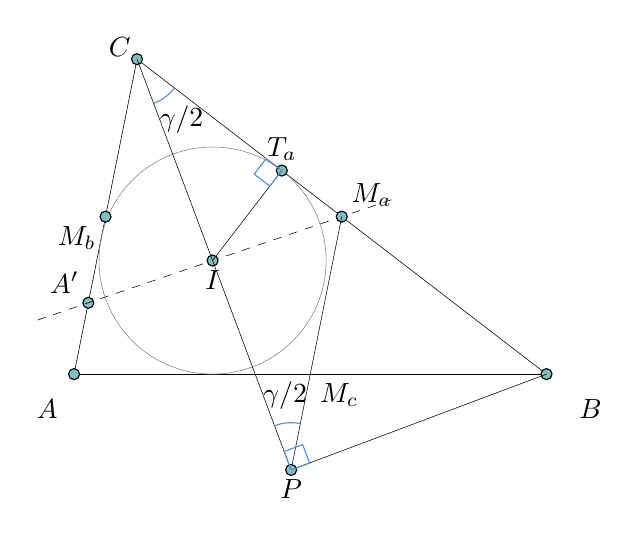
\begin{tikzpicture}[color= cackithi]
				\tkzSetUpPoint[size=4, fill= teal!50]
				
				\tkzDefPoints{0/0/A,6/0/B,0.8/4/C}
				
				\tkzDefTriangleCenter[centroid](A,B,C)
				\tkzGetPoint{G}
				\tkzDefSpcTriangle[medial](A,B,C){Ma,Mb,Mc}
				%\tkzLabelPoints(A,B,C)
				\tkzDefTriangleCenter[in](A,B,C)
				\tkzGetPoint{I}
				
				\tkzDefCircle[in](A,B,C) 
				\tkzGetPoints{I}{i}
				
				\tkzInterLL(Mb,I)(B,C)
				\tkzGetPoint{B1}
				\tkzInterLL(Ma,I)(A,C)
				\tkzGetPoint{A1}
				\tkzDrawSegments(A,B B,C C,A)
				\tkzDrawPoint(A1)
				\tkzLabelPoint[above left](A1){$A'$}
				\tkzDrawLine[dashed](A1,Ma)
				\tkzDrawCircle(I,i)
				\tkzDrawPoints(I, Mb, Ma)
				
				\tkzDrawPoints(A,B,C)
				
				\tkzLabelPoint(I){$I$}
				
				\tkzAutoLabelPoints[center = G](A,B,C)
				\tkzLabelPoint[below left](Mb){$M_b$}
				\tkzLabelPoint[above right](Ma){$M_a$}
				\tkzLabelPoint[below right](Mc){$M_c$}
				\tkzInterLL(C,I)(Ma,Mc)
				\tkzGetPoint{P}
				\tkzDrawSegments(C,P P,B Ma,P)
				\tkzDrawPoint(P)
				\tkzLabelPoint(P){$P$}
				\tkzDefPointBy[projection = onto C--B](I)
				\tkzGetPoint{Ta}
				\tkzDrawPoint(Ta)
				\tkzLabelPoint[above](Ta){$T_a$}
				\tkzDrawSegment(Ta,I)
				\tkzMarkRightAngles(C,Ta,I C,P,B)
				\tkzMarkAngle[size = 0.6, arc=l](P,C,B)
				\tkzLabelAngle[pos=0.95](P,C,B){$\gamma/2$}
				\tkzMarkAngle[size = 0.6, arc=l](Ma,P,C)
				\tkzLabelAngle[pos=0.95](Ma,P,C){$\gamma/2$}
			\end{tikzpicture}}
			\vspace*{-10pt}
		\end{figure}
		Gọi $T_a$ là điểm tiếp xúc của đường tròn nội tiếp tam giác $ABC$ với cạnh $BC$ thì $CT_a = (a+b-c)/2$. Do đó 
		\begin{align*}
			CI = \frac{CT_a}{\cos(\gamma/2)} = \frac{a+b-c}{2 \cos(\gamma/2)}
		\end{align*}
		và ta có
		\begin{align*}
		IP = CP - CI & =  a \cos(\gamma/2) - \frac{a+b-c}{2 \cos(\gamma/2)} \\
		& = \frac{2a \cos^2(\gamma/2) -a-b+c}{2 \cos(\gamma/2)} \\
		& = \frac{a[2\cos^2(\gamma /2)-1] - b +c}{2 \cos(\gamma/2)} \\
		& = \frac{a \cos (\gamma)-b+c}{2 \cos(\gamma/2)}.
		\end{align*}
		Vì $A'C \parallel M_aP$ nên theo định lý Thales 
		\begin{align*}
			\frac{CA'}{M_aP} = \frac{CI}{IP} & =  \frac{a+b-c}{a \cos(\gamma) - b +c} \\
			& = \frac{a+b-c}{a\frac{a^2 + b^2 -c^2}{2ab} -b +c} \\
			& = \frac{2b(a+b-c)}{a^2 + b^2 - c^2 - 2b^2 + 2bc} \\
			& = \frac{2b(a+b-c)}{a^2 - b^2 -c^2 + 2bc} \\
			& = \frac{2b(a+b-c)}{(a+c-b)(a+b-c)} \\
			& = \frac{2b}{a+c-b}
		\end{align*}
		và do đó
		\begin{align*} 
			\frac{CA'}{CB} = \frac{CA'}{2M_aP} = \frac{b}{a+c-b}. \tag{$3$}
		\end{align*}
		Hoán đổi vai trò của $A$ với $B$ (do đó $M_a$ với $M_b$, $a$ với $b$, $A'$ với $B'$) ta thu được
		\begin{align*} 
			\frac{CB'}{CA} = \frac{a}{b+c-a}. \tag{$4$}
		\end{align*}
		Từ giả thiết hai tam giác $ABC$ và $A'B'C$ có cùng diện tích ta có
		\begin{align*}
			\frac{CA'}{CB} = \frac{CA}{CB'}.
		\end{align*}
		Kết hợp với ($3$) và ($4$) ta nhận được
		\begin{align*}
			&\frac{b}{a+c-b}  = \frac{b+c-a}{a} \\
			\Leftrightarrow \,&ab  = (a+c-b)(b+c-a) \\
			\Leftrightarrow \,&ab  = c^2 - (a-b)^2 \\
			\Leftrightarrow \,&c^2 = a^2 + b^2 - ab.
		\end{align*}
		Từ hệ thức $c^2 = a^2 + b^2 - 2 ab \cos(\gamma)$ suy ra $\cos(\gamma) = \frac{1}{2}$. Do đó $\gamma = 60^{\circ}$.
	\vskip 0.1cm
	\textbf{\color{cackithi}Câu $\pmb{4}$}: Cho một đa giác đều $2n$ cạnh. Trong các đoạn thẳng nối các đỉnh của đa giác (cạnh biên hoặc đường chéo) ta tô $n$ đoạn màu đỏ sao cho:
	\vskip 0.1cm
	$1.$ Các điểm cuối của các đoạn màu đỏ chính là $2n$ đỉnh của đa giác.
	\vskip 0.1cm
	$2.$ Không có $2$ đoạn màu đỏ nào có độ dài bằng nhau.
	\vskip 0.1cm
	Tìm tất cả các số tự nhiên $n \ge 2$ sao cho tồn tại một phép tô màu thỏa mãn yêu cầu bên trên.
	\vskip 0.1cm	
	\textit{Lời giải.}
	Ta sẽ chứng minh rằng một cách tô màu như vậy tồn tại khi và chỉ khi $n \equiv 0 \mod 4$ hoặc $n \equiv 1 \mod 4$.
	\vskip 0.1cm
	$``\Rightarrow":$ Giả sử tồn tại cách tô màu như vậy. Gọi $2n$ đỉnh của đa giác là $A_1, A_2, \ldots, A_{2n}$, được sắp xếp theo chiều kim đồng hồ. Ta định nghĩa \textit{khoảng cách $d(i,j)$ giữa hai đỉnh $A_i, A_j$} là số cạnh nằm trên đường đi ngắn nhất dọc theo các cạnh biên của đa giác nối hai đỉnh này. Khoảng cách này sẽ lấy một trong các giá trị trong tập $\{1,2\ldots,n\}$. Chẳng hạn, với $n=4$ như trong Hình $2$ thì $d(1,4) = 3$ và $d(1,7) = 2$. 
	\vskip 0.1cm
	Dễ thấy
	\begin{align*}
		A_iA_j = 2r \sin\frac{d(i,j)\pi}{2n}
	\end{align*}
	với $r$ là khoảng cách từ đỉnh đến tâm của đa giác. Do đó, $A_iA_j > A_rA_s \iff d(i,j) > d(r,s)$. Bởi vậy ta có thể thay yêu cầu rằng không có hai đoạn màu đỏ nào có cùng độ dài bằng yêu cầu không có hai cặp đỉnh nào có cùng khoảng cách.
	\vskip 0.1cm	
	Biểu diễn mỗi cặp đỉnh $(A_i, A_j)$ bởi cặp chỉ số $(i,j)$. Ta có thể giả sử $i <j$. Bài toán đã cho tương đương với việc phân hoạch tập $2n$ số tự nhiên $\{1,2,\ldots, 2n\}$ thành $n$ cặp $\{(i_k,j_k)\}_{k = 1}^n$ với $i_k<j_k$ sao cho tập các khoảng cách $\{d(i_k,j_k)\}_{k=1}^n$ là $\{1, \ldots, n\}$. Ta có
	\begin{align*}
		\hspace*{-10pt}d(i_k,j_k) \!\!=\!\! 
		\begin{cases}
			\!\!j_k\!-\!i_k, \text{ nếu } j_k\!-\!i_k \!\le\! n \\
			\!\!2n\!-\! j_k \!+\! i_k, \text{ nếu } j_k\!-\!i_k \!>\! n.
		\end{cases}\hspace*{-10pt} \tag{$5$}
	\end{align*}
	Bằng cách hoán đổi $i_k$ với $j_k$ trong trường hợp $j_k-i_k > n$ ta có 
	\begin{align*} 
			\sum_{k=1}^{n}j_k - \sum_{k=1}^n i_k = &\sum_{k=1}^nd(i_k,j_k) + 2ns\\
			 = &\sum_{k=1}^ni + 2ns \\
			 = &n(n+1)/2 + 2ns.\tag{$6$}
		\end{align*}
		với $s$ là số trường hợp $j_k-i_k > n$. Mặt khác,
		\begin{align*}
			\sum_{k=1}^nj_k + \sum_{k=1}^ni_k &= \sum_{k=1}^{2n}i \\
			&= 2n(2n+1)/2. \tag{$7$}
		\end{align*}
		Từ các phương trình ($6$) và ($7$) ta thu được 
		\begin{align*}
			\sum_{k=1}^{n}j_k = \frac{n(5n+3)}{4} + ns.
		\end{align*}
		Vì $\sum_{k=1}^{n}j_k \in \mathbb{N}$ nên $\frac{n(5n+3)}{4} \in \mathbb{Z}$. Từ đó suy ra $n \equiv 0 \mod 4$ hoặc $n \equiv 1 \mod 4$.
		\vskip 0.1cm
		$``\Leftarrow":$
		\vskip 0.1cm
		\underline{\textit{Trường hợp $n \equiv 0 \mod 4$.}} Đặt $n = 4k$.
		\vskip 0.1cm
		$\bullet$ Với $k=1$ ta có thể tô màu như Hình $2$.
			\begin{figure}[H]
%				\vspace*{-10pt}
				\centering
				\captionsetup{labelformat= empty, justification=centering}
				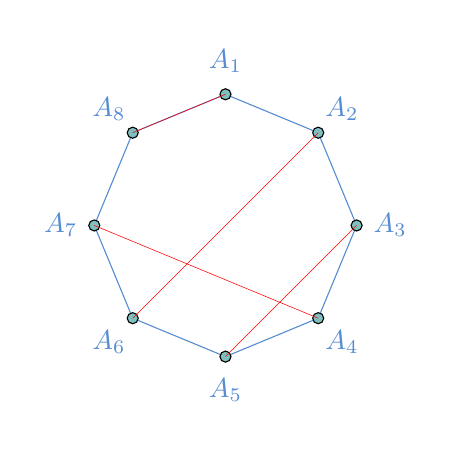
\begin{tikzpicture}[cackithi,scale = 0.75]
					\tkzSetUpPoint[size=4, fill= teal!50]
					\def\laenge{1.7}
					\def\n{8}
					\pgfmathtruncatemacro\w{360/\n}
					\draw
					(0:0) coordinate (A1)
					foreach \i in {2,...,\n}
					{--++(360+\w/2-\i*\w +\w:\laenge) coordinate (A\i)}
					--cycle;
					\tkzDrawPoints(A1,A...,A8)
					\foreach \i in {1,...,\n}\node[anchor={270-\i*\w +\w}, circle] at (A\i){$A_{\i}$};
					\tkzDrawSegment[red](A1,A8)
					\tkzDrawSegment[red](A2,A6)
					\tkzDrawSegment[red](A3,A5)
					\tkzDrawSegment[red](A4,A7)
				\end{tikzpicture}
				\caption{\small\textit{\color{cackithi}Hình $2$. Đa giác đều $8$ cạnh.}}
				\vspace*{-10pt}
			\end{figure}
			$\bullet$ Với $k \ge 2$ thì danh sách các đoạn màu đỏ cùng với khoảng cách giữa các đỉnh (phương trình ($5$) với $2n = 8k$) được cho trong bảng dưới đây:
		\begin{center}
			\resizebox{\linewidth}{!}{%
				\begin{tabular}{ |c|c|c| } 
					\hline
					Chỉ số & Cạnh & Khoảng cách \\ 
					\hline
					$1 \le i \le k$ & $(i, 8k+1-i)$ & $1,3, \ldots, 2k-1$ \\ 
					\hline
					$i = k+1$ & $(k+1, 5k+1)$ & $4k$ \\
					\hline
					$k+2 \le i \le 2k$ & $(i, 8k+2-i)$ & $2k+2, 2k+4, \ldots, 4k-2$ \\ 
					\hline
					$i = 2k+1$ & $(2k+1,4k+1)$ & $2k$ \\
					\hline
					$2k+2 \le i \le 3k+1$ & $(i, 8k+3-i)$ & $4k-1, 4k-3,\ldots, 2k+1$ \\
					\hline
					$3k+2 \le i \le 4k$ & $(i, 8k+2-i)$ & $2k-2, \ldots, 2$ \\
					\hline
			\end{tabular}}
		\end{center}
		\begin{figure}[H]
%			\vspace*{-5pt}
			\centering
			\captionsetup{labelformat= empty, justification=centering}
			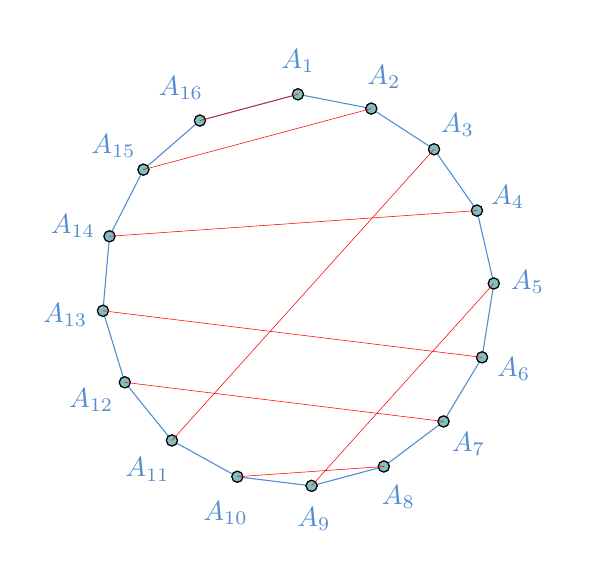
\begin{tikzpicture}[cackithi,scale = 0.95]
				\tkzSetUpPoint[size=4, fill= teal!50]
				\def\laenge{1}
				\def\n{16}
				\pgfmathtruncatemacro\w{360/\n}
				\draw
				(0:0) coordinate (A1)
				foreach \i in {2,...,\n}
				{--++(360+\w/2-\i*\w +\w:\laenge) coordinate (A\i)}
				--cycle;
				\tkzDrawPoints(A1,A...,A16)
				\foreach \i in {1,...,\n}\node[anchor={270-\i*\w +\w}, circle] at (A\i){$A_{\i}$};
				\tkzDrawPoints(A1,A...,A16)
				\tkzDrawSegment[red](A1,A16)
				\tkzDrawSegment[red](A2,A15)
				\tkzDrawSegment[red](A3,A11)
				\tkzDrawSegment[red](A4,A14)
				\tkzDrawSegment[red](A5,A9)
				\tkzDrawSegment[red](A6,A13)
				\tkzDrawSegment[red](A7,A12)
				\tkzDrawSegment[red](A8,A10)
			\end{tikzpicture}
			\caption{\small\textit{\color{cackithi}Hình $3$. Đa giác đều $16$ cạnh.}}
			\vspace*{-15pt}
		\end{figure}
		\underline{\textit{Trường hợp $n \equiv 1 \mod 4$.}} Đặt $n = 4k+1$. 
		\vskip 0.1cm
		$\bullet$ Với $k=1$ ta có thể tô màu như Hình $4$.
		\begin{figure}[H]
			\vspace*{-10pt}
			\centering
			\captionsetup{labelformat= empty, justification=centering}
			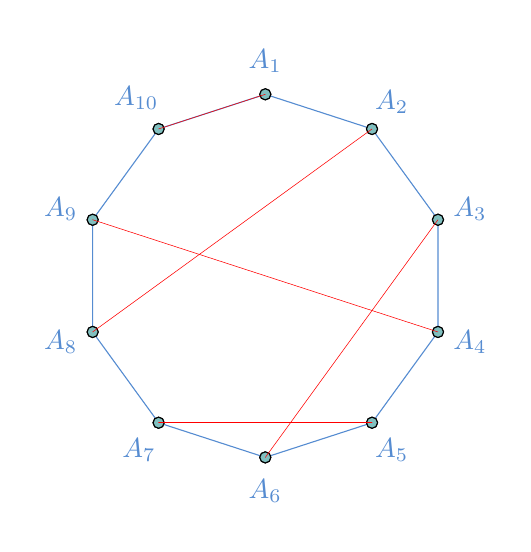
\begin{tikzpicture}[cackithi,scale = 0.95]
				\tkzSetUpPoint[size=4, fill= teal!50]
				\def\laenge{1.5}
				\def\n{10}
				\pgfmathtruncatemacro\w{360/\n}
				\draw
				(0:0) coordinate (A1)
				foreach \i in {2,...,\n}
				{--++(360+\w/2-\i*\w +\w:\laenge) coordinate (A\i)}
				--cycle;
				\tkzDrawPoints(A1,A...,A10)
				\foreach \i in {1,...,\n}\node[anchor={270-\i*\w +\w}, circle] at (A\i){$A_{\i}$};
				\tkzDrawPoints(A1,A...,A10)
				\tkzDrawSegment[red](A1,A10)
				\tkzDrawSegment[red](A2,A8)
				\tkzDrawSegment[red](A3,A6)
				\tkzDrawSegment[red](A4,A9)
				\tkzDrawSegment[red](A5,A7)
			\end{tikzpicture}
			\caption{\small\textit{\color{cackithi}Hình $4$. Đa giác đều $10$ cạnh.}}
			\vspace*{-15pt}
		\end{figure}
		$\bullet$  Với $k \ge 2$ thì danh sách các đoạn màu đỏ cùng với khoảng cách giữa các đỉnh (phương trình ($5$) với $2n = 8k+2$) được cho trong bảng dưới đây:
		\begin{center}
			\resizebox{\linewidth}{!}{%
				\begin{tabular}{ |c|c|c| } 
					\hline
					Chỉ số & Cạnh & Khoảng cách \\ 
					\hline
					$1 \le i \le k$ & $(i, 8k+3-i)$ & $1,3, \ldots, 2k-1$ \\ 
					\hline
					$i = k+1$ & $(k+1, 5k+3)$ & $4k$ \\
					\hline
					$k+2 \le i \le 2k$ & $(i, 8k+4-i)$ & $2k+2, 2k+4, \ldots, 4k-2$ \\ 
					\hline
					$i = 2k+1$ & $(2k+1, 4k+2)$ & $2k+1$ \\
					\hline
					$2k+2 \le i \le 3k+1$ & $(i, 8k+5-i)$ & $4k+1, 4k-1,\ldots, 2k+3$ \\
					\hline
					$3k+2 \le i \le 4k+1$ & $(i,8k+4-i)$ & $2k, \ldots, 2$ \\
					\hline
			\end{tabular}}
		\end{center}
\end{multicols}
\newpage
\begingroup
\AddToShipoutPicture*{\put(150,700){\includegraphics[scale=1]{../tieude1.pdf}}}
\centering
\endgroup
\vspace*{3pt}

\begin{multicols}{2}
	Trong phần đầu chuyên mục, chúng tôi sẽ trình bày với các bạn lời giải các bài toán trong kỳ thi Olympic toán Tuymaada năm $2022$ của nước cộng hòa Sakha (Yakutia), thuộc Liên bang Nga đăng trong số tháng $5/2023$. 
	\begin{figure}[H]
		\vspace*{-5pt}
		\centering
		\captionsetup{labelformat= empty, justification=centering}
		\includegraphics[width= 1\linewidth]{gocolympic}
%		\caption{\small\textit{\color{}.}}
		\vspace*{-15pt}
	\end{figure}
	{\bf\color{cackithi} OC$\pmb{46.}$} Arnim và Brentano có một chiếc bình nhỏ đựng $1500$ viên kẹo trên bàn và một túi lớn đựng kẹo dự phòng dưới gầm bàn. Họ thay phiên nhau chơi một trò chơi với Arnim bắt đầu trước. Ở mỗi lượt đi, người chơi có thể ăn $7$ viên kẹo trong bình hoặc lấy 6 viên kẹo từ túi bên dưới và thêm chúng vào bình. Người chơi không được lấy kẹo trong túi dưới gầm bàn hai lần liên tiếp. Người chơi được tuyên bố là người chiến thắng nếu làm cho chiếc bình rỗng sau lượt chơi của mình. Trong mọi trường hợp khác, nếu
	một người chơi không thể thực hiện được nước đi trong lượt của mình, trò chơi được tuyên bố là hòa. Liệu người nào có chiến lược để luôn chiến thắng?
	\vskip 0.1cm
	\textit{Lời giải.} Ban đầu trong bình có $1500$ viên kẹo. Brentano có chiến lược để luôn thắng bằng cánh đảm bảo rằng nếu trước lượt đi của Arnim trong bình có $15k$ viên kẹo, thì sau khi mỗi người đi $2$ lượt, trong bình sẽ còn lại $15(k-1)$ viên kẹo. 
	\vskip 0.1cm
	Cụ thể là nếu trong lượt đi thứ nhất của mình Arnim thêm $6$ viên kẹo vào bình thì ở lượt đi sau anh ta phải ăn $7$ viên. Do đó Brentano sẽ ăn $7$ viên kẹo trong cả $2$ lượt đi của mình và số kẹo trong bình sau đó là $15k+6-7-7-7=15(k-1).$ Nếu trong lượt đi thứ nhất của mình Arnim  ăn $7$ viên thì Brentano cũng ăn $7$ viên trong lượt thứ nhất. 
	Đến lượt đi thứ $2$ nếu Arnim ăn $7$ viên thì sau đó Brentano thêm vào $6$ viên và số kẹo trong bình còn lại là $15k-7-7-7+6=15(k-1).$    Còn nếu đến lượt thứ $2$ Arnim thêm vào 6 viên thì sau đó Brentano sẽ ăn $7$ viên và số kẹo trong bình còn lại là $15k-7-7+6-7=15(k-1).$ Như vậy sau khi mỗi người đi $200$ lượt thì Brentano là người chiến thắng.
	\vskip 0.1cm
	{\bf\color{cackithi}OC$\pmb{47.}$}  Cho $M$ là trung điểm của cạnh $A$B trong tam giác đều $ABC.$ Điểm $D$ thuộc cạnh $BC$ sao cho $BD : DC = 3 : 1.$ Giả sử $T$ là điểm trên đường thẳng đi qua $C$ và song song với $MD$ sao cho $\angle CTA = 150^\circ.$ Tìm số đo $\angle MTD.$
	\begin{figure}[H]
		\vspace*{-5pt}
		\centering
		\captionsetup{labelformat= empty, justification=centering}
		\definecolor{qqwuqq}{rgb}{0.,0.39215686274509803,0.}
		\definecolor{uuuuuu}{rgb}{0.26666666666666666,0.26666666666666666,0.26666666666666666}
		\definecolor{ududff}{rgb}{0.30196078431372547,0.30196078431372547,1.}
		\begin{tikzpicture}[cackithi,scale=1.2,node font=\small]
			\draw[color=uuuuuu] (1.8771681255350392,1.9481399025612232) -- (1.90851486019539,2.1110223138105475) -- (1.7456324489460657,2.1423690484708984) -- (1.7142857142857149,1.979486637221574) -- cycle; 
			\draw [shift={(1.7142857142857149,1.979486637221574)},color=qqwuqq,fill=qqwuqq,fill opacity=0.10000000149011612] (0,0) -- (-130.8933946491309:0.23457748258628952) arc (-130.8933946491309:-10.893394649130876:0.23457748258628952) -- cycle;
			\draw  (2.,0.) circle (2.cm);
			\draw  (2.,3.4641016151377553)-- (2.5,2.5980762113533165);
			\draw  (2.3109450177226596,3.0662755356334794) -- (2.1890549822773426,2.9959022908575927);
			\draw  (3.,1.7320508075688776)-- (2.5,2.5980762113533165);
			\draw  (2.689054982277343,2.129876887073154) -- (2.8109450177226605,2.2002501318490406);
			\draw  (3.,1.7320508075688776)-- (3.5,0.8660254037844388);
			\draw  (3.3109450177226583,1.3342247280646016) -- (3.1890549822773413,1.263851483288715);
			\draw  (3.5,0.8660254037844388)-- (4.,0.);
			\draw  (3.8109450177226587,0.4681993242801627) -- (3.6890549822773417,0.3978260795042762);
			\draw  (0.,0.)-- (2.,0.);
			\draw  (0.9706778146767137,0.07037324477588658) -- (0.9706778146767137,-0.07037324477588658);
			\draw  (1.029322185323286,0.07037324477588658) -- (1.029322185323286,-0.07037324477588658);
			\draw  (2.,0.)-- (4.,0.);
			\draw  (2.9706778146767134,0.07037324477588658) -- (2.9706778146767134,-0.07037324477588658);
			\draw  (3.0293221853232857,0.07037324477588658) -- (3.0293221853232857,-0.07037324477588658);
			\draw  (2.5,2.5980762113533165)-- (2.,0.);
			\draw  (3.,1.7320508075688776)-- (2.,0.);
			\draw  (2.5756061103843018,0.8562325387809366) -- (2.453716074938985,0.9266057835568232);
			\draw  (2.5462839250610156,0.8054450240120545) -- (2.4243938896156987,0.8758182687879411);
			\draw  (1.7142857142857149,1.979486637221574)-- (3.,1.7320508075688776);
			\draw  (2.,3.4641016151377553)-- (1.7142857142857149,1.979486637221574);
			\draw  (1.7142857142857149,1.979486637221574)-- (0.,0.);
			\draw  (2.,0.)-- (1.7142857142857149,1.979486637221574);
			\draw  (1.7916802919345747,0.9506685609177279) -- (1.9309831895863658,0.9707752022822663);
			\draw  (1.7833025246993495,1.0087114349393076) -- (1.9226054223511404,1.0288180763038461);
			\draw  (1.7142857142857149,1.979486637221574)-- (2.5,2.5980762113533165);
			\draw  (2.0636107016266734,2.3440746880399277) -- (2.1506750126590424,2.233488160534963);
%			\begin{scriptsize}
				\draw [fill=white] (0.,0.) circle (1.5pt);
				\draw[color=ududff] (-0.17754689709133267,-0.15347137061022087) node {$A$};
				\draw [fill=white] (4.,0.) circle (1.5pt);
				\draw[color=ududff] (4.23250977553091,-0.16520024473953532) node {$B$};
				\draw [fill=white] (2.,3.4641016151377553) circle (1.5pt);
				\draw[color=uuuuuu] (2.086125809866361,3.6818704696755975) node {$C$};
				\draw [fill=white] (2.,0.) circle (1.5pt);
				\draw[color=uuuuuu] (2.0157525650904744,-0.21211574125679306) node {$M$};
				\draw [fill=white] (3.,1.7320508075688776) circle (1.5pt);
				\draw[color=uuuuuu] (3.1769111038926074,1.922539350278433) node {$R$};
				\draw [fill=white] (2.5,2.5980762113533165) circle (1.5pt);
				\draw[color=uuuuuu] (2.649111768073456,2.8022049099770157) node {$D$};
				\draw [fill=white] (3.5,0.8660254037844388) circle (1.5pt);
				\draw[color=uuuuuu] (3.3763019640909535,0.6558209443124747) node {$F$};
				\draw [fill=white] (1.7142857142857149,1.979486637221574) circle (1.5pt);
				\draw[color=uuuuuu] (1.5935130964351534,2.1688457069940363) node {$R'$};
				\draw (2.2386011735474494,1.7700639865973455) node[below] {$120^{\circ}$};
%			\end{small}
		\end{tikzpicture}
		\vspace*{-5pt}
	\end{figure}
	\textit{Lời giải.} Gọi $\ell$ là đường thẳng đi qua $C$ song song với $MD.$ Giả sử đường tròn đường kính $AB$ cắt $BC$ tại $R$ và cắt $\ell$ tại $R'.$  Ta sẽ chứng minh  $R'$ trùng với  $T.$ 
	\vskip 0.1cm
	Dễ thấy tam giác cân $MBR$ có góc $\angle MBR=60^\circ$ nên nó là tam giác đều. Do đó $R$ là trung điểm $BC$ và $D$ là trung điểm $RC.$ Trong tam giác $CRR',$ $MD$ đi qua trung điểm của $CR$ và song song $CR'$ nên nó phải đi qua trung điểm của $RR'.$ Do $MD$ là đường kính, ta suy ra $MD\perp RR'.$ Do $CR'$ song song với $MD,$ ta suy ra $\angle CR'R=90^\circ.$ 
	\vskip 0.1cm
	Mặt khác, do $\angle AR'R=180^\circ - \angle ABR= 180^\circ-60^\circ=120^\circ,$ ta có 
	\begin{align*}
		\angle AR'C&=360^\circ-\angle AR'R - \angle CR'R \\
		&= 360^\circ -120^\circ - 90^\circ=150^\circ.
	\end{align*}
	Như vậy $R'$ trùng với $T.$ Do $R$ và $R'$ đối xứng nhau qua $MD$ ta có $\angle MR'D=\angle MRD= 120^\circ.$  Như vậy $\angle MTD=120^\circ.$  
	\vskip 0.1cm
	{\bf\color{cackithi} OC$\pmb{48.}$} Cho các số nguyên $a, b, c$ và số nguyên tố lẻ $p.$ Chứng minh rằng tồn tại các số nguyên $x$ và $y$ sao cho $p$ là ước của $x^2 + y^2 + ax + by + c.$      
	\vskip 0.1cm
	\textit{Lời giải.}
	Khi tính giá trị  $f(x)=x^2+ax+c$ modulo $p,$ với $x \in \{0, 1, \cdots, p - 1\}$ ta được ít nhất $\frac{p+1}{2}$  số phân biệt. Thật vậy, nếu $x_1$ và $x_2$ là hai số nguyên phân biệt nằm giữa $0$ và $p-1$, và $p$ là ước của  $f(x_1)-f(x_2) = x_1^2 +ax_1+c-(x_2^2 +ax_2+c) = (x_1-x_2)(x_1+x_2+a)$,
	thì $p$ cũng là ước của $x_1 + x_2 + a$, nghĩa là với mỗi $x_1\in \{0, 1, \cdots, p - 1\}$ có nhiều nhất
	một $x_2\in \{0, 1, \cdots, p - 1\}$  sao cho $f(x_2)\equiv f(x_1) \mod p.$ 
	\vskip 0.1cm
	Lập luận tương tự cho thấy các giá trị của đa thức $g(y) = -y^2 - by$ với  $y \in \{0, 1, \cdots, p - 1\}$ ta cũng nhận được ít nhất $\frac{p+1}{2}$ số phân biệt modulo $p.$ Như vậy, ta có hai tập các số dư modulo $p,$  mỗi tập có nhiều hơn $\frac{p}{2}$ số dư, do đó hai tập này phải có ít nhất một phần tử chung. Ta suy ra $p$ là ước của $f(x) - g(y)$ với các số nguyên $x$ và $y$ nào đó. Ta được điều cần chứng minh.  
	\vskip 0.1cm
	Trong phần cuối của chuyên mục kỳ này, chúng tôi sẽ giới thiệu với bạn đọc ba bài toán chọn lọc trong kỳ thi Olympic toán vùng Trung Mỹ và Caribê năm $2023$. Các bài toán này phù hợp với trình độ học sinh lớp $8-10$.
	\vskip 0.1cm
	{\bf\color{cackithi} OC$\pmb{55.}$} Tìm tất cả các cách tô màu các số nguyên dương sao cho điều kiện sau thỏa mãn:  
	\vskip 0.1cm
	$\bullet$ Mỗi số có màu xanh hoặc đỏ;
	\vskip 0.1cm
	$\bullet$ Tổng của hai số (không nhất thiết phân biệt) cùng màu bất kỳ  có màu xanh.
	\vskip 0.1cm
	{\bf\color{cackithi} OC$\pmb{56.}$} Octavio viết một số nguyên dương $n$ lên bảng  và sau đó anh bắt đầu một quá trình trong đó, ở mỗi bước, anh xóa số nguyên $k$ được viết trên bảng  và thay thế nó bằng một trong các số sau:
	\begin{align*}
		3k-1, \quad 2k+1, \quad \frac{k}{2},
	\end{align*}
	với điều kiện số mới viết là số nguyên.
	\vskip 0.1cm
	Chứng minh rằng với mọi số nguyên dương $n$, Octavio có thể viết lên bảng  số $3^{2023}$ sau hữu hạn bước.
	\vskip 0.1cm
	{\bf\color{cackithi} OC$\pmb{57.}$} Trong một cái ao có $n (n \geq 3)$  hòn đá  xếp thành vòng tròn. Một công chúa muốn đánh số những hòn đá với các số $1, 2, \dots, n$ theo thứ tự nào đó rồi đặt một số con cóc lên những hòn đá. Sau khi đặt tất cả các con cóc vào vị trí, chúng bắt đầu nhảy theo quy tắc sau: khi một con cóc đến hòn đá có đánh số $k$, nó đợi $k$ phút rồi nhảy sang hòn đá liền kề theo chiều kim đồng hồ.
	\vskip 0.1cm
	Hỏi số lượng cóc nhiều nhất là bao nhiêu để công chúa có thể đánh số các hòn đá và đặt các con cóc sao cho không bao giờ có hai con cóc ở trên cùng một hòn đá trong thời gian từ một phút trở lên?
\end{multicols}
%	\newpage

%	\setcounter{figure}{0}
%	\thispagestyle{diendandayvahoctoannone}
\pagestyle{diendandayvahoctoan}
\everymath{\color{diendantoanhoc}}
\graphicspath{{../diendantoanhoc/pic/}}
\blfootnote{$^1$\color{diendantoanhoc}Trường PT Hermann Gmeiner Vinh, Nghệ An.}
\begingroup
\AddToShipoutPicture*{\put(0,616){\includegraphics[width=19.3cm]{../bannerdiendan}}}
\AddToShipoutPicture*{\put(110,555){\includegraphics[scale=1]{../tieude1111.pdf}}}  
\centering
\endgroup
\vspace*{160pt} 

\textit{\textbf{\color{diendantoanhoc}LTS.} Trong số này, tạp chí Pi giới thiệu đến bạn đọc một bài viết đạt giải trong kỳ thi Bài giảng và bài viết Toán học, mang tên Hoàng Tuỵ, năm $2022$. Bài viết về chủ đề giảng dạy Toán theo chương trình Toán học $2018$ -- Chương trình Giáo dục Phổ thông mới.}
\begin{multicols}{2}
	\textbf{\color{diendantoanhoc}I.	Đặt vấn đề}
	\vskip 0.1cm
	Trong quá trình tìm các Bài toán thực tế, và xem trò chơi dân gian ``Ô ăn quan" chúng tôi phát hiện ra có sự tương đồng rất lớn giữa bài toán tập hợp hữu hạn với tập hợp các viên sỏi trong trò chơi ``Ô ăn quan". Từ đó chúng tôi nghĩ đến câu hỏi có thể sử dụng phương pháp ô ăn quan để giải các bài Toán tập hợp đếm được, hữu hạn hay không? Áp dụng cho một số Bài toán ban đầu chúng tôi thấy cách giải là rất đẹp và dễ hiểu. Chúng tôi đặt tên cho cách giải đó là ``phương pháp ô ăn quan"
	\vskip 0.1cm
	Với ý muốn là sẽ tạo một cách giải hết sức trực quan chúng tôi quyết định nghiên cứu sâu hơn về các Bài toán tập hợp được phát biểu dưới dạng các bài Toán cổ, ngoài ra chúng ta có thể giải quyết được một số bài ở mức độ phức tạp hơn, khi chứa nhiều biến trong một bài toán.
	\vskip 0.1cm
	Môn toán trong chương trình phổ thông ở cấp Tiểu học giúp học sinh có những kiến thức cơ bản và sơ giản ban đầu về số học, hình học, các yếu tố đại lượng và hình thành các kĩ năng toán học góp phần xây dựng phương pháp học tập, làm việc có kế hoạch, chủ động, sáng tạo giúp các em học tập tốt các môn học khác trong nhà trường và chuẩn bị cho các bậc học tiếp theo. Trong bài viết này, chúng tôi sẽ giải một lớp các Bài toán đó bằng phương pháp ``Ô ăn quan",các ví dụ đưa ra là những bài toán rất quen thuộc ở Tiểu học và cả một số bài tập đề cập ở trên chương trình Toán THPT.
	\vskip 0.1cm
	Với ý tưởng như trên, bài viết sẽ trình bày những kết quả đạt được đạt được trong quá trình chuyển tải phương pháp ``Ô ăn quan" vào giải các bài Toán tập hợp của chương trình Toán Phổ thông mới.
	\vskip 0.1cm
	\textbf{\color{diendantoanhoc}II.	Giải các Bài toán tập hợp bằng phương pháp ``Ô ăn quan"}
	\vskip 0.1cm
	Các bài toán cổ dưới đây thường có nhiều phương pháp giải mà mỗi bậc học có thể được trang bị một cách khác nhau. Tuy nhiên đây là các bài toán có tính logic cao nên học sinh phải có năng lực Toán học khá mới dùng được các phương pháp như vẽ biểu đồ, đặt ẩn giải hệ phương trình, hoặc dùng biểu đồ Venn. Trong phương pháp ô ăn quan, chúng tôi sử dụng những mô tả rất thực tế qua việc dùng những viên sỏi; ô trống và rải sỏi dẫn đến học sinh không cần đòi hỏi quá nhiều kiến thức về Toán vẫn có thể lĩnh hội được.
	\vskip 0.1cm
	\textbf{\color{diendantoanhoc}Bài toán $\pmb{1}$: Gà và chó}
	\begin{center}
		``Vừa gà vừa chó,\\
		Bó lại cho tròn,\\
		$36$ con, $100$ chân chẵn."
	\end{center}
	Hỏi có bao nhiêu con gà, bao nhiêu con chó?
	\vskip 0.1cm
	\textit{Lời giải.}
	Theo bài ta có: tổng số con gà và con chó có tất cả $36$ con và $100$ chân.
	\vskip 0.1cm
	Bây giờ ta vẽ $36$ ô và dùng $100$ viên sỏi. Trong $36$ ô, mỗi ô ta rải vào $2$ viên sỏi hết $72$ viên sỏi, còn lại $28$ viên sỏi. Rải tiếp $28$ viên sỏi còn lại vào các ô, mỗi ô thêm $2$ viên sỏi. Khi đó, có $14$ ô chứa $4$ viên sỏi và $22$ ô chứa $2$ viên sỏi. Vậy ta có $14$ con chó và $22$ con gà.
	\begin{figure}[H]
		\vspace*{-5pt}
		\centering
		\captionsetup{labelformat= empty, justification=centering}
		\includegraphics[width= 1\linewidth]{1}
		\vspace*{-15pt}
	\end{figure}
	\textbf{\color{diendantoanhoc}Bài toán $\pmb2$: Thuyền to -- Thuyền nhỏ}
	\begin{center}
		``Thuyền to chở được $6$ người,\\
		Thuyền nhỏ chở được $4$ người là đông.\\
		Một đoàn trai gái sang sông,\\
		$10$ thuyền to nhỏ giữa dòng đang trôi.\\
		Toàn đoàn có cả $100$ người, Trên bờ còn $48$ người đợi sang"
	\end{center}
	Hỏi có bao nhiêu thuyền to, bao nhiêu thuyền nhỏ
	\vskip 0.1cm
	\textit{Lời giải}.
	Toàn đoàn có $100$ người, trên bờ còn $48$ người đợi sang, như vậy có $52$ người đang ngồi trên $10$ thuyền.
	\vskip 0.1cm
	Theo bài ta có: Tổng số thuyền nhỏ và to là $10$ thuyền, $52$ người.
	\vskip 0.1cm
	Bây giờ ta vẽ $10$ ô và dùng $52$ viên sỏi. Trong $10$ ô mỗi ô ta rải vào $4$ viên sỏi hết $40$ viên sỏi, còn lại $12$ viên sỏi. Bỏ tiếp $12$ viên sỏi còn lại vào các ô, mỗi ô thêm $2$ viên. Khi đó, có $6$ ô chứa $6$ viên sỏi và $4$ ô chứa $4$ viên sỏi. Hay có $6$ thuyền to và $4$ thuyền nhỏ.
	\begin{figure}[H]
		\vspace*{5pt}
		\centering
		\captionsetup{labelformat= empty, justification=centering}
		\includegraphics[width= 1\linewidth]{2}
		\vspace*{-15pt}
	\end{figure}
	\textit{Nhận xét.}
	Thông qua những ví dụ trên ta thấy phương pháp ô ăn quan sử dụng những trực quan cụ thể, giúp học sinh dễ dàng thực hiện và ghi nhớ cách làm đồng thời tìm ra kết quả chính xác.
	\vskip 0.1cm
	Ví dụ trên đã yêu cầu học sinh vận dụng được sự mềm dẻo, linh hoạt trong suy nghĩ để giải quyết bài toán. Đó là một yếu tố rất cần thiết, tránh sự cứng nhắc rập khuôn theo những phương pháp đã dẫn đến những cách giải cồng kềnh hoặc bế tắc.
	\vskip 0.1cm
	\textbf{\color{diendantoanhoc}Bài toán $\pmb3$: Bài toán lợn và gà}
	\begin{center}
		Tối qua đếm đàn lợn gà\\
		Thấy được trăm mắt còn đầu năm mươi\\
		Một trăm hai chục chân tròn\\
		Đố bạn biết có bao nhiêu gà và lợn?
	\end{center}
	\textit{Lời giải.}
	Có $50$ cái đầu nên tổng số lợn và gà là $50$ con và tổng số là $120$ chân. Bây giờ ta vẽ $50$ ô tượng trưng cho $50$ con, và lấy $120$ viên sỏi tượng trưng cho $120$ cái chân.
	\vskip 0.1cm
	Bây giờ ta sẽ rải đầy kín tất cả các ô, với mỗi ô hoặc hai viên sỏi, hoặc $4$ viên sỏi. Khi đó số ô có $4$ viên tức là có $4$ chân chính là lợn, số ô có $2$ viên tức là có $2$ chân chính là gà.
	\vskip 0.1cm
	Rõ ràng khi rải đầy các ô có hai viên mỗi ô, thì hết $100$ viên, nên thừa $20$ viên, $20$ viên còn lại rải đủ cho $10$ ô, và do đó để thêm mỗi ô $2$ viên. Vậy số ô có $4$ viên là $10$ nên số lợn là $10$ con, còn lại số ô có $2$ viên là $40$ ô vậy có $40$ gà.
	\begin{figure}[H]
		\vspace*{-5pt}
		\centering
		\captionsetup{labelformat= empty, justification=centering}
		\includegraphics[width= 1\linewidth]{3}
		\vspace*{-15pt}
	\end{figure}
	\textbf{\color{diendantoanhoc}Bài toán $\pmb4$: Bài toán ``Thương nhau cau sáu bổ ba"}
	\begin{center}
		`Thương nhau cau sáu bổ ba\\
		Ghét nhau cau sáu bổ ra làm mười.\\
		Mỗi người một miếng trăm người,\\
		Có mười bảy quả hỏi người ghét yêu"?
	\end{center}
	Hỏi có bao nhiêu quả cau ghét và bao nhiêu quả cau yêu.
	\vskip 0.1cm
	\textit{Lời giải.}
	Ta coi $17$ quả cau là $17$ ô vuông và $100$ miếng cau chia cho $100$ người là $100$ viên sỏi. Trong $17$ ô vuông, mỗi ô vuông rải $3$ viên sỏi hết $51$ viên sỏi, còn lại $49$ viên sỏi. Rải tiếp $49$ viên còn lại vào các ô, mỗi ô thêm $7$ viên. Khi đó, có $7$ ô chứa $10$ viên sỏi và $10$ ô chứa $3$ viên sỏi. Hay có $30$ người tương ứng với $10$ quả cau bổ $3$ và $70$ người ghét ứng với $7$ quả cau bổ $10$.
	\begin{figure}[H]
		\vspace*{-5pt}
		\centering
		\captionsetup{labelformat= empty, justification=centering}
		\includegraphics[width= 1\linewidth]{4}
		\vspace*{-15pt}
	\end{figure}
	\textbf{\color{diendantoanhoc}Bài toán $\pmb6$: (Buôn cà phê)}
	\vskip 0.1cm
	Người nọ mua một số cafe tốt và một số cafe xấu trộn lại cân nặng $50$ kg, trả tất cả $7.800\$$. Biết rằng giá $1$ kg cafe tốt $180\$$, giá $1$ kg cafe xấu $120\$$. Hỏi người ấy mua mỗi hạng cafe mấy kg?
	\vskip 0.1cm
	\textit{Lời giải}.
	Ta coi mỗi ô là $1$ kg cà phê, có $50$ kg cà phê nên sẽ có $50$ ô, bây giờ ta sẽ xem mỗi viên sỏi là $60\$$, tổng cộng là $7800\$$ nên sẽ ứng với $130$ viên sỏi. Sau đó ta sẽ rải sỏi vào các ô, mà mỗi ô chỉ nhận $2$ viên $=120\$$ hoặc $3 $viên $=180\$$, số ô có $3$ viên chính là cà phê tốt, số ô chỉ có $2$ viên chính là cà phê xấu. Đầu tiên ta rải đủ $50$ ô, mỗi ô $2$ viên thì còn lại $30$ viên, ta tiểp tục rải $30$ viên còn lại mỗi ô thêm $1$ viên cho đến khi hết sỏi. Ta có hình vẽ sau.
	\begin{figure}[H]
		\vspace*{5pt}
		\centering
		\captionsetup{labelformat= empty, justification=centering}
		\includegraphics[width= 1\linewidth]{5}
		\vspace*{-15pt}
	\end{figure}
	Nhìn vào bảng ta thấy có $30$ ô chứa $3$ viên sỏi, vậy có $30$ kg cà phê tốt, có $20$ ô chứa hai viên sỏi nên có $20$ kg cà phê xấu.
	\vskip 0.1cm
	Bây giờ ta sẽ giải các bài Toán tập hợp có độ phức tạp cao hơn, đó là những bài toán và có từ $3$ biến trở lên. Những bài toán này nếu giải bằng các cách thông thường sẽ hết sức phức tạp và đòi hỏi rất nhiều kỹ thuật. Nhưng với phương pháp ``Ô ăn quan" ta sẽ có một lời giải rất dễ hiểu, đẹp đẽ và học sinh Tiểu học cũng có thể hiểu được.
	\vskip 0.1cm
	\textbf{\color{diendantoanhoc}Bài toán $\pmb7$:}
	\vskip 0.1cm
	Lớp $5A$ có $35$ học sinh (HS) làm bài kiểm tra toán cuối Kỳ II. Đề bài gồm có $3$ bài toán. Giáo viên chủ nhiệm lớp báo cáo với Nhà trường rằng: Cả lớp mỗi em đều làm được ít nhất một bài, trong đó $20$ em giải được bài toán thứ nhất, $14$ HS giải được bài toán thứ hai, $10$ HS giải được bài toán thứ ba, $5$ HS giải được bài toán thứ hai và thứ ba, $2$ HS giải được bài toán thứ nhất và thứ hai, chỉ có một HS được $10$ điểm vì đã giải được cả ba bài. Học sinh nào giải được bài $3$ thì làm ít nhất thêm được một bài khác.
	Hỏi lớp học đó có bao nhiêu HS không dự kiểm tra?
	\vskip 0.1cm
	\textit{Lời giải}.
	Trước hết ta vẽ bảng gồm có $35$ ô ứng với $35$ em học sinh lớp $5A$. Ta lấy $20$ tấm thẻ ký hiệu là số $B1$ ứng với số lần giải được bài toán $1$, lấy $14$ thẻ ký hiệu là $B2$ ứng với $14$ lần giải được bài toán $2$, $10$ tấm thẻ đánh dấu là $B3$ ứng với $10$ lượt giải được bài toán $3$. Bây giờ ta sẽ rải thẻ vào các ô theo quy tắc đã cho. Đầu tiên ta rải $20$ tấm thẻ $B1$ vào $20$ ô, sau đó ta rải đến tấm thẻ $B2$ vào $2$ ô có thẻ $B1$ và thêm $12$ ô trống, hết thẻ $B2$ bây giờ ta rải thẻ $B3$, $1$ tấm thẻ vào ô đã có $2$ thẻ $B1$ và $B2$, tiếp tục rải $5$ thẻ vào các ô chỉ có thẻ $B2$, do làm được bài $3$ thì sẽ làm được hơn một bài do đó sẽ rải $4$ thẻ còn lại vào các ô chỉ có $B1$. Sau khi rải hết thẻ mà ô nào còn trống có nghĩa là học sinh đó không đi thi.
	\begin{figure}[H]
		\vspace*{-5pt}
		\centering
		\captionsetup{labelformat= empty, justification=centering}
		\includegraphics[width= 1\linewidth]{6}
		\vspace*{-15pt}
	\end{figure}	
	Nhìn vào bảng sau khi rải hết các thẻ theo quy tắc trên ta thấy còn lại chỉ có $3$ ô trống nên có $3$ em học sinh không tham gia thi cuối kỳ II.
	\begin{figure}[H]
		\vspace*{-5pt}
		\centering
		\captionsetup{labelformat= empty, justification=centering}
		\includegraphics[width= 1\linewidth]{7}
		\vspace*{-15pt}
	\end{figure}
	\textbf{\color{diendantoanhoc}Bài toán $\pmb8$:} 
	\vskip 0.1cm
	Trong một hội nghị có $100$ đại biểu tham dự, mỗi đại biểu nói được một hoặc hai trong ba thứ tiếng: Nga, Anh hoặc Pháp. Có $39$ đại biểu chỉ nói được tiếng Anh, $35$ đại biểu nói được tiếng Pháp, có $12$ đại biểu biết $2$ thứ tiếng trong đó $8$ đại biểu nói được cả tiếng Anh và tiếng Nga. Hỏi có bao nhiêu đại biểu chỉ nói được tiếng Nga, bao nhiêu đại biểu chỉ nói được tiếng Pháp?
	\vskip 0.1cm
	\textit{Lời giải}.
	\begin{figure}[H]
		\vspace*{-5pt}
		\centering
		\captionsetup{labelformat= empty, justification=centering}
		\includegraphics[width= 1\linewidth]{8}
		\vspace*{-15pt}
	\end{figure}
	Ta vẽ $100$ ô tương ứng với $100$ đại biểu. Ta sẽ làm $39$ thẻ chữ $A$ ứng với $35$ người nói được tiếng Anh, $35$ thẻ chữ $P$ ứng với $35$ người biết nói tiếng Pháp và $8$ thẻ chữ $NA$ ứng với số lượng biết nói tiếng Nga, gọi thẻ chữ $N$ là ký hiệu biết nói tiếng Nga.
	\vskip 0.1cm
	Đầu tiên, ta sẽ rải $39$ thẻ $A$ vào $39$ ô. Ta rải tiếp $35$ thẻ chữ $P$ vào các ô trống tiếp theo, tiếp tục rải tiếp $8$ thẻ $NA$ vào các ô trống còn lại. Bây giờ ta sẽ rải thẻ chữ $N$, vì mỗi đại biểu nói được ít nhất một thứ tiếng, nên những ô trống còn lại ta sẽ rải chữ $N$ vào. Do có $12$ đại biểu biết nói hai thứ tiếng mà lại có $8$ người nói Anh và Nga do đó chắc chắn có $4$ người nói tiếng Pháp thì nói được tiếng Nga (vì không thể cùng biết cả Anh và Pháp) do đó ta sẽ rải $4$ thẻ chữ $N$ vào $4$ ô có chữ $P$. Khi đó ô nào mà chỉ có một mình chữ N là chỉ nói được tiếng Nga, những ô chỉ có chữ $P$ là chỉ nói được tiếng Pháp. Nhìn vào bảng ta thấy: có $18$ ô chữ $N$ vậy có $18$ đại biểu chỉ nói được tiếng Nga. Có $31$ ô chỉ có chữ $P$ nên có $31$ đại biểu chỉ nói được tiếng Pháp
	\vskip 0.1cm
	\textbf{\color{diendantoanhoc}Bài toán $\pmb9$.}
	\vskip 0.1cm
	$50$ bạn học sinh lớp $12A$ đều đội $1$ trong hai loại mũ: Mũ cứng hoặc mũ mềm, đi $1$ trong $2$ loại giày đen hoặc nâu, mặc $1$ trong $2$ loại áo: trắng hoặc xanh. Có $18$ bạn đội mũ mềm, $19$ bạn đi giầy đen, $11$ bạn có áo trắng. Hỏi có thể chắc chắn có ít nhất bao nhiêu bạn vừa đi giày nâu, vừa đội mũ cứng và mặc áo xanh?
	\vskip 0.1cm
	\textit{Lời giải}.
	Ta sẽ vẽ bảng gồm $50$ ô, ta kí hiệu thẻ chữ $M$, $C$ lần lượt ứng với đội mũ mềm và mũ cứng, thẻ $Đ$, $N$ lần lượt cho giày đen và giày nâu, thẻ $T$, $X$ cho mặc áo trắng và áo xanh.
	\begin{figure}[H]
		\vspace*{-5pt}
		\centering
		\captionsetup{labelformat= empty, justification=centering}
		\includegraphics[width= 1\linewidth]{9}
		\vspace*{-15pt}
	\end{figure}
	Vì có $18$ bạn đội mũ mềm ta rải $18$ thẻ $M$ vào $18$ ô, các ô trống còn lại ta rải chữ $C$ cho các bạn đội mũ cứng, ta rải tiếp $19$ thẻ $D$ vào hết các bạn có thẻ chữ $C$, hết chữ $C$ ta sẽ rải sang chữ $M$, nhiều ô chữ $C$ nhất có thể. Sau đó ta rải $11$ thẻ chữ $T$ vào ô chữ $CN$, hết các ô đó ta sẽ rải sang các ô còn lại, khi hết $11$ thẻ chữ $T$ ta tiếp tục rải chữ $X$ vào tất cả các ô không chứa chữ $T$. Khi đó ô nào mà chữa $3$ chữ $CNX$ thì đó chính là học sinh đi giày Nâu, đội mũ Cứng và mặc áo Xanh.
	\vskip 0.1cm
	Nhìn vào bảng ta thấy chỉ có hai ô có $3$ chữ $CNX$ nên có ít nhất $2$ học sinh đội mũ cứng, đi giày nâu và mặc áo xanh.
	\vskip 0.1cm
	\textit{Nhận xét:} Đây là bài Toán logic khá hóc búa vì nó chứa đến $6$ yếu tố để tác động lên một học sinh, nếu dùng phương pháp suy luận thông thường chúng ta sẽ vấp phải các lý luận khá phức tạp và dễ bị nhầm lẫn. Phương pháp ``Ô ăn quan" cho ta một lời giải rất đẹp đẽ và khá ngắn gọn.
	\vskip 0.1cm
	\textbf{\color{diendantoanhoc}IV. Bài tập đề xuất}
	\vskip 0.1cm
	\textbf{\color{diendantoanhoc}Bài $\pmb1$:} Trong một Hội nghị có $100$ người tham dự, trong đó có $10$ người không biết tiếng Nga và tiếng Anh, có $75$ người biết tiếng Nga và $83$ người biết Tiếng Anh. Hỏi trong hội nghị có bao nhiêu người biết cả $2$ thứ tiếng Nga và Anh?
	\vskip 0.1cm
	\textbf{\color{diendantoanhoc}Bài $\pmb2$:} Một lớp học có $16$ học sinh học giỏi môn Toán; $12$ học sinh học giỏi môn Văn; $8$ học sinh vừa học giỏi môn Toán và Văn; $19$ học sinh không học giỏi cả hai môn Toán và Văn. Hỏi lớp học có bao nhiêu học sinh?
	\vskip 0.1cm
	\textbf{\color{diendantoanhoc}Bài $\pmb3$:} Một lớp có $45$ học sinh. Mỗi em đều đăng ký chơi ít nhất một trong hai môn: bóng đá và bóng chuyền. Có $35$ em đăng ký môn bóng đá, $15$ em đăng ký môn bóng chuyền. Hỏi có bao nhiêu em đăng ký chơi cả $2$ môn?
	\vskip 0.1cm
	\textbf{\color{diendantoanhoc}Bài $\pmb4$:} Lớp $12A$ có $20$ học sinh thích bóng đá, $17$ học sinh thích bơi, $36$ học sinh thích bóng chuyền, $14$ học sinh thích bơi và bóng đá, $13$ học sinh thích bơi và bóng chuyền, $15$ học sinh thích bóng đá và bóng chuyền, $10$ học sinh thích cả $3$, $12$ học sinh không thích môn nào cả . Tính số học sinh của lớp $12A$?
	\vskip 0.1cm
	\textbf{\color{diendantoanhoc}Bài $\pmb5$:} Lớp $10A$ có $40$ học sinh trong đó có $10$ bạn học sinh giỏi Toán, $15$ bạn học sinh giỏi Lý, và $22$ bạn không giỏi môn học nào trong hai môn Toán, Lý. Hỏi lớp 10A có bao nhiêu bạn học sinh vừa giỏi Toán vừa giỏi Lý?
	\vskip 0.1cm
	\textbf{\color{diendantoanhoc}Bài $\pmb6$:} (Thi giữa kỳ $1$ -- Trường PTTH Lý Nhân Tông, Hà Nội) Lớp $10A$ có $45$ học sinh trong đó có $15$ học sinh thích chơi đá bóng, $12$ học sinh thích chơi bóng rổ, $6$ học sinh thích chơi cả $2$ môn. Số học sinh không thích chơi cả $2$ môn thể thao trên là:
	\vskip 0.1cm
	\textbf{\color{diendantoanhoc}Bài $\pmb7$:} Lớp $10A$ có $7$ học sinh giỏi Toán, $5$ học sinh giỏi Lý, $6$ học sinh giỏi Hóa, $3$ học sinh giỏi cả Toán và Lý, $4$ học sinh giỏi cả Toán và Hóa, $2$ học sinh giỏi cả Lý và Hóa, $1$ học sinh giỏi cả $3$ môn Toán, Lý, Hóa. Số học sinh giỏi đúng hai môn học của lớp 10A là bao nhiêu.
	\vskip 0.1cm
	\textbf{\color{diendantoanhoc}Tài liệu tham khảo}
	\vskip 0.1cm
	[$1$]	L. V. An, N. T. Sơn, N. T. Thiêm, N. T. H. Anh, N. Q. Chung ($2023$), Nhìn bài toán cổ theo quan điểm Tổ hợp, Kỷ yếu HTKH cấp Trường: ``Nâng cao chất lượng đào tạo ngành Sư phạm trong bối cảnh hiện nay", Trường Đại học Hà Tĩnh, (Hà Tĩnh, ngày $24/3/2023$), $179 - 186$.
	\vskip 0.1cm
	[$2$] Naum Yakolevich Vilenkin -- Dịch giả: Nguyễn Tiến Dũng, Trần Thanh Nam, Nguyễn Chí Thức, Hồ Thị Thảo Trang, \textit{Toán học qua các câu chuyện về Tập hợp}, Tủ sách SPUTNIK, NXB Thế giới, năm $2017$.
	\vskip 0.1cm
	[$3$] Trịnh Hồng Long, \textit{$670$ bài toán đố}, NXB Sống Mới, năm $1970$.
	\vskip 0.1cm
	[$4$] Người dịch: Trần Lưu Cường, Trần Lưu Thịnh, \textit{Những bài toán cổ}, NXB giáo dục, năm $1995$.
	\vskip 0.1cm
	[$4$] Trần Nam Dũng (Tổng chủ biên), Trần Đức Huyên (Chủ biên), Nguyễn Thành Anh -- Vũ Như Thư Hương -- Ngô Hoàng Long -- Phạm Hoàng Quân -- Phạm Thị Thu Thủy, \textit{Sách chân trời sáng tạo -- Toán $10$ -- Tập $1$}, NXB giáo dục Việt Nam, năm $2022$.
	\vskip 0.1cm
	[$5$]	Đỗ Đức Thái (Tổng chủ biên), Phạm Xuân Chung, Nguyễn Sơn Hà, Nguyễn Thị Phương Loan, Phạm Sỹ Nam, Phạm Minh Phương, Phạm Hoàng Quân, \textit{Sách Cánh diều -- Toán $10$ -- Tập $1$}, NXB Giáo dục, năm $2021$	
\end{multicols}
%	\newpage
	
%	\thispagestyle{empty}
%	\begingroup 
%	\AddToShipoutPicture*{\put(0,0){\includegraphics[width=19.5cm]{thumoi.pdf}}}
%	\centering
%	\vspace*{0cm}
%	\endgroup
%	\newpage	
%	\pagestyle{empty}
%
%	\setcounter{figure}{0}
%	\thispagestyle{timhieukhoahocnone}
\pagestyle{timhieukhoahoc}
\everymath{\color{timhieukhoahoc}}
\blfootnote{$^1$\text{\color{timhieukhoahoc}https://phys.org/news/2023-10-scientists-nobel-prize-physics-electrons.html}}
\blfootnote{$^2$\text{\color{timhieukhoahoc}Viện Toán học.}}

\graphicspath{{../timhieukhoahoc/pic/}}
\begingroup
\AddToShipoutPicture*{\put(0,616){\includegraphics[width=19.3cm]{../bannertimhieu}}}
\AddToShipoutPicture*{\put(60,533){\includegraphics[scale=1]{../tieude.pdf}}}
\centering
\endgroup
\vspace*{170pt}

\begin{multicols}{2}
	Hôm thứ ba ngày $3$ tháng $10$ vừa qua, ba nhà khoa học đã giành được Giải Nobel Vật lý $2023$ nhờ mang đến cho chúng ta cái nhìn đầu tiên về thế giới siêu tốc độ của các electron quay tít, một lĩnh vực có thể sẽ giúp cải tiến các thiết bị điện tử hoặc chẩn đoán bệnh.
	\begin{figure}[H]
		\vspace*{-5pt}
		\centering
		\captionsetup{labelformat= empty, justification=centering}
		\includegraphics[width= 1\linewidth]{1}
		\caption{\small\textit{\color{timhieukhoahoc}Ảnh: Viện Hàn lâm Khoa học Hoàng gia Thụy~Điển.}}
		\vspace*{-10pt}
	\end{figure}
	Giải thưởng được trao cho nhà vật lý Pháp -- Thụy Điển Anne L'Huillier, nhà vật lý người Pháp Pierre Agostini và nhà vật lý gốc Hungary Ferenc Krausz, vì công trình của họ về thành phần tí hon chạy quanh hạt nhân của nguyên tử và là cái cơ bản của hầu như mọi thứ: hóa học, vật lý, cơ thể và vật dụng của chúng ta.
	\vskip 0.1cm
	Theo các chuyên gia, electron di chuyển nhanh đến nỗi con người không thể cô lập được chúng, nhưng bằng cách quan sát trong những tích tắc nhỏ nhất có thể, các nhà khoa học hiện đã có cái nhìn thoáng qua ``mờ mờ" về chúng, qua đó mở ra nhiều ngành khoa học hoàn toàn mới.
	\vskip 0.1cm
	``Electron di chuyển rất nhanh, và chúng thực sự là lực lượng lao động ở mọi nơi," Mats Larsson, thành viên Ủy ban Giải thưởng Nobel, cho biết. ``Một khi có thể điều khiển và hiểu được electron, bạn đã tiến được một bước lớn."
	\vskip 0.1cm
	L'Huillier, giáo sư tại Đại học Lund, Thụy Điển, là người phụ nữ thứ năm được Nobel Vật lý.
	\vskip 0.1cm
	``Gửi đến tất cả phụ nữ, tôi muốn nói rằng nếu bạn thích, nếu bạn có một chút đam mê với những thách thức kiểu này, hãy theo đuổi nó," bà nói với hãng tin AP.
	\vskip 0.1cm
	\textbf{\color{timhieukhoahoc}Khám phá được trao Giải Nobel Vật lý}
	\vskip 0.1cm
	Ba nhà khoa học, độc lập với nhau, đã sử dụng xung laser ngày càng nhanh để bắt lại hoạt động của nguyên tử xảy ra ở tốc độ chóng mặt -- một phần tỷ tỷ giây, hay một \textit{atto} giây\footnote[3]{\color{timhieukhoahoc}$1$ atto giây = $10^{-18}$ giây -- Pi.} -- giống như cách các nhiếp ảnh gia sửa dụng cửa trập tốc độ cao để chụp ảnh chim ruồi đang hút mật hoa.
	\begin{figure}[H]
		\vspace*{5pt}
		\centering
		\captionsetup{labelformat= empty, justification=centering}
		\includegraphics[width= 1\linewidth]{3}
		\caption{\small\textit{\color{timhieukhoahoc}Nhà vật lý Pháp--Thụy Điển Anne L'Huillier}}
		\vspace*{-10pt}
	\end{figure}
	Khoảng thời gian đó ngắn đến mức nào?
	\vskip 0.1cm
	``Hãy lấy một giây, là khoảng thời gian của một nhịp tim," chủ tịch Ủy ban Giải thưởng Nobel, Eva Olsson nói. Để đạt đến cỡ atto giây, cần chia nó cho $1000$ sáu lần.
	\vskip 0.1cm
	Nhà vật lý Mark Pearce, thành viên Ủy ban Giải thưởng Nobel, nói rằng ``số atto giây trong một giây bằng số giây đã trôi qua kể từ Big Bang, khoảng $13{,}8$ tỷ năm trước."
	\vskip 0.1cm
	Nhưng ngay cả khi ``thấy" được electron, các nhà khoa học cũng không thấy được hết.
	\vskip 0.1cm
	``Bạn có thể thấy nó ở phía bên này hay phía bên kia của một phân tử," L'Huillier, năm nay $65$ tuổi, nói. ``Nó vẫn rất mờ."
	\vskip 0.1cm
	``Electron giống sóng, như sóng trên mặt nước, nhiều hơn là giống hạt, và cái chúng tôi đo với kỹ thuật của mình là vị trí của ngọn sóng," bà nói thêm.
	\vskip 0.1cm
	\textbf{\color{timhieukhoahoc}Vì sao electron quan trọng?}
	\vskip 0.1cm
	Electron có vai trò then chốt vì chúng chính là ``cách các nguyên tử liên kết với nhau," L'Huillier nói. Đó là nơi diễn ra các phản ứng hóa học.
	\vskip 0.1cm
	``Dù ta không thể thấy chúng, electron hiện diện khắp mọi nơi trong cuộc sống của chúng ta, theo cả nghĩa cuộc sống sinh học lẫn cuộc sống kỹ thuật, cuộc sống hàng ngày," Krausz nói tại một buổi họp báo. ``Trong cuộc sống sinh học, electron tạo nên chất keo giữa các nguyên tử, từ đó các nguyên tử tạo thành phân tử, và các phân tử này là những viên gạch nhỏ nhất để xây dựng nên mọi cơ thể sống."
	\vskip 0.1cm
	Và nếu muốn hiểu cách chúng làm việc, bạn cần biết cách chúng di chuyển, Krausz nói.
	\vskip 0.1cm
	Hiện tại, khoa học này phục vụ cho việc tìm hiểu vũ trụ của chúng ta, nhưng người ta hy vọng nó cuối cùng sẽ có ứng dụng thực tế trong điện tử, chẩn đoán bệnh và hóa học cơ bản.
	\vskip 0.1cm
	L'Huillier nói rằng công trình của bà cho thấy tầm quan trọng của việc tiến hành nghiên cứu cơ bản mà không cần biết có ứng dụng trong tương lai hay không: bà đã làm việc với nó $30$ năm trước khi những ứng dụng thực tế trở nên rõ ràng hơn.
	\begin{figure}[H]
		\vspace*{-5pt}
		\centering
		\captionsetup{labelformat= empty, justification=centering}
		\includegraphics[width= 1\linewidth]{2}
		\caption{\small\textit{\color{timhieukhoahoc}Anne L'Huillier trả lời phỏng vấn tại Đại học Lund, Lund, Thụy Điển hôm thứ ba $3/10/2023$.}}
		\vspace*{-10pt}
	\end{figure}
%	\end{figure}
%	\begin{figure}[H]
%		\vspace*{-5pt}
%		\centering
%		\captionsetup{labelformat= empty, justification=centering}
%		\includegraphics[width= 1\linewidth]{4}
%		%		\caption{\small\textit{\color{}}}
%		\vspace*{-15pt}
%	\end{figure}
	\textbf{\color{timhieukhoahoc}Phản ứng của ba nhà khoa học}
	\vskip 0.1cm
	Khi nhận được cuộc gọi báo tin được giải thưởng, L'Huillier đang dạy vật lý cơ bản dành cho kỹ sư cho khoảng $100$ sinh viên tại Lund; điện thoại của bà để ở chế độ im lặng và bà không nghe máy. Bà kiểm tra điện thoại trong giờ giải lao và gọi lại cho Ủy ban Giải thưởng Nobel.
	\vskip 0.1cm
	Sau đó bà quay lại dạy tiếp.
	\vskip 0.1cm
	``Lúc ấy tôi đang rất tập trung, tôi quên đi Giải Nobel và cố kết thúc bài giảng của mình," bà nói với AP. Bà kết thúc bài giảng sớm một chút để có thể trả lời họp báo công bố giải thưởng tại Viện Hàn lâm Khoa học Hoàng gia Thụy Điển ở Stockholm.
	\vskip 0.1cm
	``Đây là giải thưởng cao quý nhất và tôi thật hạnh phúc được nhận nó. Thật không thể tin được," bà nói ở buổi họp báo. ``Các bạn biết đấy, không có nhiều phụ nữ được giải này, bởi thế nó rất đặc biệt."
	\vskip 0.1cm
	Ban tổ chức giải Nobel đăng trên tài khoản mạng xã hội của mình một bức ảnh L'Huillier đang nghe điện thoại.
	\begin{figure}[H]
		\vspace*{-5pt}
		\centering
		\captionsetup{labelformat= empty, justification=centering}
		\includegraphics[width= 1\linewidth]{7}
		\caption{\small\textit{\color{timhieukhoahoc}Nhà vật lý người Hungary Ferenc Krausz.}}
		\vspace*{-10pt}
	\end{figure}
	``Cảnh báo: nhà giáo tận tâm!" bài đăng trên Twitter, nay là X, viết. ``Đến cả giải Nobel Vật lý $2023$ cũng không thể kéo Anne L'Huillier khỏi sinh viên của bà."
	\vskip 0.1cm
	Và L'Huillier cho biết khi đó vẫn phải giữ bí mật về giải thưởng nên bà không được phép giải thích với sinh viên, nhưng họ đoán được.
	\vskip 0.1cm
	Agostini, giáo sư danh dự tại Đại học Bang Ohio, khi đó đang ở Paris; Ủy ban Giải thưởng Nobel không liên lạc được với ông trước khi công bố việc ông được giải với cả thế giới.
	\vskip 0.1cm
	``Tôi không nhận được cuộc gọi nào từ ủy ban giải thưởng. Có lẽ không đúng. Tôi không biết," ông cười khi trả lời AP. ``Tôi nghĩ họ tìm tôi ở Columbus\footnote[4]{\color{timhieukhoahoc}Thủ phủ bang Ohio -- Pi.}."
	\vskip 0.1cm
	``Chắc chắn có nhiều người trẻ hơn đánh giá cao giải thưởng này hơn tôi," vị giáo sư $82$ tuổi nói đùa. ``Nó cũng tốt đấy, nhưng với tôi thì hơi muộn."
	\vskip 0.1cm
	Nhưng, ông nói thêm: ``Tôi không nghĩ mình sẽ xứng đáng nếu được trao giải sớm hơn!"
	\vskip 0.1cm
	Krausz, thuộc Viện Quang học Lượng tử Max Planck và Đại học Ludwig Maximilian tại Munich, nói với các phóng viên rằng ông bị choáng ngợp.
	\vskip 0.1cm
	``Từ $11$ giờ sáng đến giờ tôi vẫn đang nghĩ xem mình đang ở trong hiện thực hay trong một giấc mơ dài," nhà vật lý $61$ tuổi nói.
	\vskip 0.1cm
	Cuộc gọi từ ủy ban giải thưởng được hiển thị ``không có ID người gọi" và thường thì Krausz không nghe những cuộc gọi như vậy, nhưng lần này, ông ``nghĩ rằng mình sẽ thử nghe, và rõ ràng không thể dập máy ngay."
	\vskip 0.1cm
	Năm ngoái, cùng với nhà khoa học Paul Corkum của Đại học Ottawa, Krausz và L'Huillier được trao giải thưởng vật lý cao quý Wolf vì những công trình của họ. Giải Nobel chỉ được trao cho không quá ba người, và Krausz nói rằng thật đáng tiếc khi nó không thể được trao cho Corkum.
	\vskip 0.1cm
	Corkum là chìa khóa đối với cách đo các xung laser xảy ra trong tích tắc, và điều này mang tính cốt yếu, Krausz nói.
	\begin{figure}[H]
		\vspace*{-5pt}
		\centering
		\captionsetup{labelformat= empty, justification=centering}
		\includegraphics[width= 1\linewidth]{5}
		\caption{\small\textit{\color{timhieukhoahoc}Ferenc Krausz trong một buổi thuyết trình tại Viện Quang học Lượng tử Max Planck, Munich, Đức hôm thứ ba $3/10/2023$.}}
		\vspace*{-15pt}
	\end{figure}
	Giải Nobel có giá trị tiền thưởng khoảng $1$ triệu đô--la Mỹ, được trao theo di chúc của người sáng lập ra nó, nhà phát minh người Thụy Điển Alfred Nobel.
	\vskip 0.1cm
	Giải Nobel Vật lý được công bố một ngày sau khi hai nhà khoa học được giải Nobel Y học -- Sinh lý học vì những khám phá giúp tạo ra vaccine mRNA cho COVID--$19$.
	\vskip 0.1cm
	\textbf{\color{timhieukhoahoc}Thông báo của Ủy ban Giải thưởng Nobel:}
	\vskip 0.1cm
	Viện Hàn lâm Khoa học Hoàng gia Thụy Điển quyết định trao giải Nobel Vật lý $2023$ cho
	\vskip 0.1cm
	\textbf{\color{timhieukhoahoc}Pierre Agostini}, Đại học Bang Ohio, Columbus, Mỹ
	\vskip 0.1cm
	\textbf{\color{timhieukhoahoc}Ferenc Krausz},  Viện Quang học Lượng tử Max Planck, Garching và Đại học Ludwig Maximilian tại Munich, Đức
	\vskip 0.1cm
	\textbf{\color{timhieukhoahoc}Anne L'Huillier}, Đại học Lund, Thụy Điển
	\vskip 0.1cm
	``vì các phương pháp thực nghiệm tạo ra các xung ánh sáng atto giây nhằm nghiên cứu động lực học của electron trong vật chất".
	\begin{figure}[H]
		\vspace*{-5pt}
		\centering
		\captionsetup{labelformat= empty, justification=centering}
		\includegraphics[width= 1\linewidth]{9}
%		\caption{\small\textit{\color{}}}
		\vspace*{-15pt}
	\end{figure}
	\textbf{\color{timhieukhoahoc}Thí nghiệm với ánh sáng bắt được những khoảnh khắc ngắn nhất}
	\vskip 0.1cm
	Ba nhà khoa học được giải Nobel Vật lý $2023$ được vinh danh vì những thí nghiệm cung cấp cho nhân loại những công cụ mới để khám phá thế giới của electron bên trong nguyên tử và phân tử. Pierre Agostini, Ferenc Krausz và Anne L'Huillier đã trình bày một cách tạo ra những xung ánh sáng cực ngắn có thể được dùng để đo các quá trình rất nhanh, trong đó electron di chuyển hoặc thay đổi năng lượng.
	\vskip 0.1cm
	Các sự kiện tốc độ cao chảy vào với nhau khi được quan sát bởi con người, giống như một đoạn phim gồm những hình ảnh tĩnh được nhìn thấy như chuyển động liên tục. Nếu muốn tìm hiểu về những sự kiện thực sự ngắn ngủi, chúng ta cần những công nghệ đặc biệt. Trong thế giới của electron, những thay đổi xảy ra chỉ trong vài chục atto giây -- một atto giây là một khoảng thời gian rất ngắn, ngắn đến nỗi số atto giây trong một giây bằng số giây tính từ khi vũ trụ ra đời.
	\vskip 0.1cm
	Những thí nghiệm của các nhà khoa học được giải đã tạo ra các xung ánh sáng ngắn đến cỡ atto giây, từ đó cho thấy các xung này có thể được sử dụng để cung cấp những hình ảnh về các quá trình bên trong nguyên tử và phân tử.
	\vskip 0.1cm
	Năm $1987$, Anne L'Huillier phát hiện thấy nhiều sóng hài bậc cao khác nhau xuất hiện khi bà truyền laser hồng ngoại qua một khí hiếm. Mỗi sóng hài bậc cao là một sóng ánh sáng mà mỗi chu kỳ của ánh sáng laser bằng một bội của chu kỳ của sóng hài. Chúng được sinh ra do laser tương tác với các phân tử khí; nó cung cấp năng lượng cho một số electron, và năng lượng dư thừa này được phát lại dưới dạng ánh sáng. Anne L'Huillier tiếp tục tìm hiểu hiện tượng này, đặt nền móng cho những đột phá tiếp theo.
	\vskip 0.1cm
	Năm $2001$, Pierre Agostini thành công trong việc tạo ra và nghiên cứu một chuỗi các xung ánh sáng liên tiếp, trong đó mỗi xung chỉ dài $250$ atto giây. Cùng lúc đó, Ferenc Krausz đang tiến hành một loại thí nghiệm khác, cho phép tách riêng một xung ánh sáng dài $650$ atto giây.
	\vskip 0.1cm
	Đóng góp của các nhà khoa học được giải cho phép nghiên cứu các quá trình diễn ra rất nhanh, mà trước đó không thể theo kịp.
	\vskip 0.1cm
	``Giờ chúng ta có thể mở cánh cửa vào thế giới của electron. Vật lý atto giây cho chúng ta cơ hội hiểu được các cơ chế do electron chi phối. Bước tiếp theo sẽ là sử dụng chúng," Eva Olsson, chủ tịch Ủy ban Giải thưởng Nobel về Vật lý, nói.
	\vskip 0.1cm
	Có nhiều ứng dụng tiềm năng trong những lĩnh vực khác nhau. Chẳng hạn, trong điện tử, việc hiểu và điều khiển được hành vi của electron trong vật liệu là rất quan trọng. Các xung atto giây cũng có thể được dùng để nhận dạng các phân tử khác nhau, thí dụ trong chẩn đoán y tế.
	\begin{figure}[H]
		\vspace*{-5pt}
		\centering
		\captionsetup{labelformat= empty, justification=centering}
		\includegraphics[width= 1\linewidth]{8}
		\caption{\small\textit{\color{timhieukhoahoc}Pierre Agostini, ảnh tại trang web khoa Vật lý, Đại học Bang Ohio.}}
		\vspace*{-10pt}
	\end{figure}
	\textbf{\color{timhieukhoahoc}Electron trong xung ánh sáng}
	\vskip 0.1cm
	Qua các thí nghiệm của mình, ba nhà khoa học được giải năm nay đã tạo được những chớp sáng đủ ngắn để chụp được chuyển động vô cùng nhanh của electron. Anne L'Huillier phát hiện ra một hiệu ứng mới từ tương tác của ánh sáng laser với các nguyên tử khí. Pierre Agostini và Ferenc Krausz cho thấy hiệu ứng này có thể được dùng để tạo ra những xung ánh sáng ngắn hơn những cái có thể được tạo ra trước đó.
	\vskip 0.1cm
	Một con chim ruồi có thể đập cánh $80$ lần mỗi giây. Chúng ta chỉ có thể nhận thấy tiếng vù vù và chuyển động mờ mờ. Với giác quan của con người, chuyển động nhanh bị mờ vào với nhau, và những sự kiện cực ngắn là không thể quan sát. Chúng ta cần đến những biện pháp công nghệ để chụp hoặc mô tả được những khoảnh khắc rất ngắn đó.
	\vskip 0.1cm
	Kỹ thuật chụp ảnh tốc độ cao và ánh sáng nhấp nháy cho phép chụp được hình ảnh chi tiết của những hiện tượng thoáng qua. Một bức ảnh rõ nét chụp một con chim ruồi đang bay đòi hỏi thời gian phơi sáng ngắn hơn nhiều so với một nhịp đập cánh của nó.
	\vskip 0.1cm
	Sự kiện càng nhanh, thời gian chụp ảnh phải càng ngắn để chụp được đúng khoảnh khắc.
	\vskip 0.1cm
	Nguyên lý tương tự được áp dụng cho tất cả các phương pháp để đo hoặc mô tả các quá trình nhanh; mọi phép đo phải được thực hiện nhanh hơn khoảng thời gian để hệ thống được quan sát trải qua một thay đổi nhận biết được, bằng không kết quả sẽ không rõ. Các nhà khoa học được giải năm nay đã tiến hành các thí nghiệm chỉ ra một phương pháp tạo ra các xung ánh sáng đủ ngắn để chụp được hình ảnh về các quá trình bên trong nguyên tử và phân tử.
	\vskip 0.1cm
	Thang thời gian tự nhiên của nguyên tử là cực kỳ nhỏ. Trong một phân tử, các nguyên tử có thể di chuyển và quay trong một phần triệu tỷ giây, hay femto giây\footnote[5]{\color{timhieukhoahoc}$1$ femto giây $= 10^{-15}$ giây -- Pi.} . Những chuyển động này có thể được nghiên cứu với những xung ngắn nhất mà một tia laser có thể tạo ra -- tuy nhiên, khi cả nguyên tử di chuyển, thang thời gian được xác định bởi hạt nhân to và nặng, vốn cực kỳ chậm so với ánh sáng và các electron nhanh nhẹn.
	\vskip 0.1cm
	Khi electron di chuyển trong nguyên tử và phân tử, chúng nhanh đến nỗi các thay đổi bị mờ sau chỉ một femto giây. Trong thế giới của electron, vị trí và năng lượng thay đổi với tốc độ từ khoảng một đến một vài trăm atto giây, tức một phần tỷ tỷ giây.
	\vskip 0.1cm
	Một atto giây ngắn đến nỗi số atto giây trong một giây bằng số giây từ khi vũ trụ sinh ra, $13{,}8$ tỷ năm trước, đến hiện tại. Để dễ hình dung, ta có thể tưởng tượng một chớp sáng đi từ một đầu căn phòng đến bức tường đối diện: nó mất mười tỷ atto giây.
	\vskip 0.1cm
	Trong một thời gian dài, một femto giây được coi là giới hạn của những chớp sáng tạo ra được.
	\vskip 0.1cm
	Việc cải tiến công nghệ sẵn có không đủ để thấy được các quá trình diễn ra trong thang thời gian ngắn đến kinh ngạc của electron; cần có một cái gì đó hoàn toàn mới. Các nhà khoa học được giải năm nay đã thực hiện những thí nghiệm mở ra lĩnh vực vật lý atto giây mới mẻ.
	\vskip 0.1cm
	\textbf{\color{timhieukhoahoc}Xung ngắn hơn nhờ các sóng hài bậc cao}
	\vskip 0.1cm
	Ánh sáng gồm những sóng -- dao động trong trường điện từ -- di chuyển trong chân không nhanh hơn mọi thứ. Sóng ánh sáng có các bước sóng khác nhau, tương đương với màu sắc khác nhau. Thí dụ, bước sóng của ánh sáng đỏ dài khoảng $700$ nm, tức khoảng một phần trăm bề rộng của một sợi tóc, và nó lặp đi lặp lại khoảng bốn trăm ba mươi nghìn tỷ lần mỗi giây. Chúng ta có thể nghĩ về xung ánh sáng ngắn nhất có thể như độ dài một chu kỳ của sóng ánh sáng, tính từ khi nó ở trên đỉnh, đi xuống đáy, rồi quay lại điểm bắt đầu. Trong trường hợp này, bước sóng dùng trong một hệ laser thông thường không thể nào đạt dưới femto giây, vì vậy trong những năm $1980$, đây được xem là một giới hạn cứng cho độ ngắn của một xung ánh sáng.
	\vskip 0.1cm
	Về mặt toán học, có thể chứng minh được rằng có thể tạo được mọi dạng sóng nếu có đủ những sóng có bước sóng và biên độ thích hợp. Bí quyết tạo ra xung atto giây là có thể tạo ra những xung ngày càng ngắn bằng cách kết hợp các bước sóng ngày càng ngắn.
	\vskip 0.1cm
	Để quan sát chuyển động của electron ở thang nguyên tử, cần các xung ánh sáng đủ ngắn, nghĩa là cần kết hợp nhiều sóng ngắn với bước sóng khác nhau.
	\vskip 0.1cm
	Để thêm bước sóng mới cho ánh sáng, cần nhiều hơn là một laser; chìa khóa dẫn đến khoảnh khắc ngắn nhất quan sát được từ trước đến nay là một hiện tượng xảy ra khi laser đi qua một chất khí. Ánh sáng tương tác với các nguyên tử khí và gây ra sóng hài bậc cao -- những sóng hoàn thành nhiều chu kỳ tương ứng với mỗi chu kỳ của sóng ban đầu. Chúng ta có thể so sánh hiện tượng này với âm bội tạo ra đặc tính của một âm thanh, giúp ta nghe được sự khác biệt của cùng một nốt khi được chơi trên ghi--ta và khi được chơi trên pi--a--nô.
	\vskip 0.1cm
	Năm $1987$, Anne L'Huillier và các đồng nghiệp tại một phòng thí nghiệm ở Pháp đã tạo được sóng hài bậc cao bằng cách sử dụng một laser hồng ngoại chiếu qua một khí hiếm. Laser hồng ngoại này tạo ra các sóng hài bậc cao ngày càng mạnh hơn so với những laser bước sóng ngắn được dùng trong các thí nghiệm trước đó. Trong thí nghiệm này, họ đã quan sát được nhiều sóng hài bậc cao với cường độ tương tự nhau.
	\vskip 0.1cm
	Trong một loạt các bài báo trong những năm $1990$, L'Huillier tiếp tục tìm hiểu hiệu ứng này, cả khi bà đã chuyển đến Đại học Lund. Những kết quả của bà đóng góp cho hiểu biết lý thuyết về hiện tượng này, đặt nền móng cho thí nghiệm đột phá tiếp theo.
	\vskip 0.1cm
	\textbf{\color{timhieukhoahoc}Electron thoát ly tạo sóng hài bậc cao}
	\vskip 0.1cm
	Khi ánh sáng laser đi qua chất khí và tác động lên các nguyên tử khí, nó tạo ra những dao động điện từ làm biến dạng điện trường giữ các electron quanh hạt nhân nguyên tử. Do đó, electron có thể thoát khỏi nguyên tử. Tuy nhiên, điện trường của ánh sáng dao động liên tục và khi nó đổi hướng, một electron đã thoát ra có thể chạy ngược về hạt nhân nguyên tử của nó. Trong chuyến du hành của mình, electron nhận thêm nhiều năng lượng từ điện trường của ánh sáng laser, và để liên kết lại với hạt nhân, nó cần giải phóng năng lượng dư thừa dưới dạng xung ánh sáng. Những xung phát ra từ electron này chính là thứ tạo ra sóng hài bậc cao được quan sát trong thí nghiệm.
	\vskip 0.1cm
	Năng lượng của ánh sáng gắn liền với bước sóng của nó. Năng lượng trong sóng hài bậc cao được phát ra tương đương với ánh sáng cực tím, vốn có bước sóng ngắn hơn ánh sáng nhìn thấy bằng mắt thường. Vì năng lượng đến từ dao động của laser, dao động của sóng hài bậc cao tỷ lệ một cách đẹp đẽ với bước sóng của xung laser ban đầu. Tương tác của ánh sáng với nhiều nguyên tử khác nhau cho kết quả là nhiều sóng ánh sáng khác nhau với những bộ bước sóng riêng.
	\vskip 0.1cm
	Khi đã được tạo ra, những sóng hài bậc cao này tương tác với nhau. Ánh sáng mạnh hơn khi các đỉnh sóng trùng nhau, và yếu hơn khi đỉnh của sóng này trùng với đáy của sóng khác. Trong những điều kiện thích hợp, các sóng hài bậc cao trùng khít với nhau, tạo ra một chuỗi các xung cực tím, mỗi xung dài vài trăm atto giây. Các nhà vật lý hiểu được lý thuyết đằng sau hiện tượng này từ những năm $1990$, nhưng đột phá trong việc xác định và kiểm nghiệm các xung này đến vào năm $2001$.
	\begin{figure}[H]
		\vspace*{-5pt}
		\centering
		\captionsetup{labelformat= empty, justification=centering}
		\includegraphics[width= 1\linewidth]{10}
		\caption{\small\textit{\color{timhieukhoahoc}Nhà vật lý Pháp  Pierre Agostini.}}
		\vspace*{-10pt}
	\end{figure}
	Pierre Agostini và nhóm nghiên cứu của ông tại Pháp đã thành công trong việc tạo ra và nghiên cứu một chuỗi các xung ánh sáng liên tiếp, như một đoàn tàu có nhiều toa. Họ sử dụng một kỹ thuật đặc biệt, đặt ``đoàn tàu xung" cùng với một phần bị lùi lại của xung laser ban đầu, để thấy được cách các sóng hài bậc cao đồng pha với nhau. Quá trình này cũng cho phép họ đo độ dài của các xung trong đoàn tàu, và họ nhận thấy mỗi xung chỉ dài $250$ atto giây.
	\vskip 0.1cm
	Cùng lúc đó, Ferenc Krausz và nhóm nghiên cứu của mình tại Áo đang nghiên cứu một kỹ thuật để chọn ra một xung riêng lẻ, như một toa được tách khỏi đoàn tàu và đặt sang một đường ray khác. Xung mà họ tách thành công dài $650$ atto giây và nhóm dùng nó để theo dõi và nghiên cứu một quá trình trong đó electron bị kéo ra khỏi nguyên tử.
	\vskip 0.1cm
	Những thí nghiệm này cho thấy các xung atto giây có thể được quan sát và đo, và chúng cũng có thể được sử dụng trong những thí nghiệm mới.
	\vskip 0.1cm
	Giờ thì thế giới atto giây đã mở ra, những xung ánh sáng ngắn này có thể được dùng để nghiên cứu chuyển động của electron. Hiện nay, người ta đã có thể tạo ra các xung chỉ dài vài chục atto giây, và những kỹ thuật này vẫn liên tục phát triển.
	\vskip 0.1cm
	\textbf{\color{timhieukhoahoc}Tiếp cận với chuyển động của electron}
	\vskip 0.1cm
	Các xung atto giây cho phép đo khoảng thời gian để kéo một electron khỏi nguyên tử, và xem xét sự phụ thuộc của khoảng thời gian này vào độ chặt chẽ của liên kết giữa electron với hạt nhân nguyên tử của nó. Ngày nay, có thể xây dựng lại cách mà phân bố electron dao động từ bên này sang bên kia hoặc từ nơi này đến nơi khác trong phân tử và vật chất; trước đây vị trí của chúng chỉ có thể được đo bằng một giá trị trung bình.
	\vskip 0.1cm
	Xung atto giây có thể được dùng để kiểm tra các quá trình nội tại của vật chất, và để nhận dạng các sự kiện khác nhau. Những xung này đã được dùng để tìm hiểu vật lý chi tiết của nguyên tử và phân tử, và chúng có những ứng dụng tiềm năng trong nhiều lĩnh vực, từ điện tử đến y học.
	\vskip 0.1cm
	Chẳng hạn, xung atto giây có thể được dùng để đẩy các phân tử, khiến chúng phát ra những tín hiệu đo được. Tín hiệu phát ra từ các phân tử có cấu trúc đặc biệt, một dạng ``vân tay" giúp nhận dạng phân tử, điều này có những ứng dụng tiềm năng, bao gồm chẩn đoán y tế.
\end{multicols}
%	\newpage
%	
%	\thispagestyle{empty}
%	\begingroup 
%	\AddToShipoutPicture*{\put(0,0){\includegraphics[width=19.45cm]{QC}}}
%	\centering
%	\vspace*{0cm}
%	\endgroup
%	\newpage	 
%	\pagestyle{empty}
%	
%	\setcounter{figure}{0}
%	 \thispagestyle{gocconone}
\pagestyle{gocco}
\everymath{\color{gocco}}
\graphicspath{{../gocco/pic/}}
\blfootnote{$^1${\color[named]{gocco}Đại kiện tướng quốc tế.}}
\begingroup
\AddToShipoutPicture*{\put(0,616){\includegraphics[width=19.3cm]{../bannergocco}}}
\AddToShipoutPicture*{\put(96,525){\includegraphics[scale=1]{../tieude.pdf}}} 
\centering
\endgroup

\vspace*{185pt}

\begin{multicols}{2}
	Lý thuyết cờ tàn cơ bản đều cho rằng xe và tượng chống xe không có tốt đều được coi là hòa cờ cơ bản. Tuy nhiên thực tế thi đấu cho thấy khả năng hòa cờ cho bên yếu không nhiều. Bên yếu cần phải chơi rất chính xác nếu muốn gỡ hòa.
	Trong bài học hôm nay, chúng tôi xin trình bày một số tình huống cơ bản 
	\vskip 0.1cm
	\textbf{\color{gocco}A.	Philidor}
	\begin{center}
		\newgame
		\fenboard{3k4/4r3/3K4/3B4/8/8/8/5R2 b Q - 0 1}
		\scalebox{0.85}\showboard
		\vskip 0.1cm
		\textit{\small\color{gocco}Hình $1$. Trắng đi trước thắng, $1749$.}
	\end{center}
	\textbf{\color{gocco}$\pmb{1}$.Xf$\pmb{8}$+ Xe$\pmb{8}$ $\pmb{2}$.Xf$\pmb{7}$ Xe$\pmb{2}$ $\pmb{3}$.Xh$\pmb{7}$} (Hình $2$) [Một nước đi chờ đợi]
	\vskip 0.1cm
	\textbf{\color{gocco}$\pmb{3}$...Xe$\pmb{1}$ $\pmb{4}$.Xb$\pmb{7}$! Xc$\pmb{1}$} [$4$...Vc$8$ $5$.Xa$7$ Xb$1$ $6$.Xh$7$! 
	\vskip 0.1cm
	$6$...Vb$8$ $7$.Xh$8$+ Va$7$ $8$.Xa$8$+ Vb$6$ $9$.Xb$8$+ Va$5$ $10$.Xxb$1$]
	\vskip 0.1cm
	\textbf{\color{gocco}$\pmb{5}$.Tb$\pmb{3}$!!} 
	\begin{center}
		\newgame
		\fenboard{2k5/7R/3K4/3B4/8/8/8/1r6 b Q - 0 1}
		\scalebox{0.85}\showboard
		\vskip 0.1cm
		\textit{\small\color{gocco}Hình $2$.}
	\end{center}
	\begin{center}
		\newgame
		\fenboard{3k4/1R6/3K4/8/8/1B6/8/2r5 b Q - 0 1}
		\scalebox{0.85}\showboard
		\vskip 0.1cm
		\textit{\small\color{gocco}Hình $3$.}
	\end{center}
	\textit{Kỹ thuật giành chiến thắng cơ bản của bên có tương là tìm cách ép vua đối phương xuống hàng ngang số $8,1$ hoặc cột a,h. Sau đó phối hợp giữa xe và tượng thực hiện vừa che chắn cho vua khỏi các nước chiếu của xe đối bằng tượng trong khi đó dùng xe đe dọa chiếu hết.}
	\vskip 0.1cm
	\textbf{\color{gocco}$\pmb{5}$...Xc$\pmb{3}$ $\pmb{6}$.Te$\pmb{6}$! Xd$\pmb{3}$+ $\pmb{7}$.Xd$\pmb{5}$} [Tượng trắng che chắn cho vua]
	\vskip 0.1cm
	$7$...Xc$3$ $8$.Xd$7$+ Vc$8$ $9$.Xh$7$ Vb$8$ $10$.Xb$7$+ Vc$8$ $11$.Xb$4$ Vd$8$ $12$.Tc$4$!! (Hình $4$). Trắng dùng Tượng ngăn cản xe đối phương phòng thủ ở ô c$8$.
	\begin{center}
		\newgame
		\fenboard{3k4/8/3K4/8/1RB5/2r5/8/8 b Q - 0 1}
		\scalebox{0.85}\showboard
		\vskip 0.1cm
		\textit{\small\color{gocco}Hình $4$.}
	\end{center}
	Trắng đe dọa chiếu hết ở nước tiếp theo
	\vskip 0.1cm
	\textbf{\color{gocco}$\pmb{12}$...Vc$\pmb{8}$} [$12$...Ve$8$ $13$.Xb$8\#$]
	\vskip 0.1cm
	\textbf{\color{gocco}$\pmb{13}$.Te$\pmb{6}$+ Vd$\pmb{8}$ $\pmb{14}$.Xb$\pmb{8}$+}
	\vskip 0.1cm
	\textbf{\color{gocco}Lolli}
	\begin{center}
		\newgame
		\fenboard{2k5/3r4/2K5/2B5/8/8/8/4R3 b Q - 0 1}
		\scalebox{0.85}\showboard
		\vskip 0.1cm
		\textit{\small\color{gocco}Hình $5$. Trắng đi trước thắng, $1763$.}
	\end{center}
	Trong rất nhiều trường hợp mặc dù xe đen cũng phòng thủ từ phía sau hoặc bên sườn, tuy nhiên bên mạnh cũng vẫn thắng.
	\vskip 0.1cm
	\textbf{\color{gocco}$\pmb{1}$.Xe$\pmb{8}$+ Xd$\pmb{8}$ $\pmb{2}$.Xe$\pmb{7}$ Xd$\pmb{2}$} [Nếu $2$...Xh$8$ $3$.Td$6$ Vd$8$ $4$.Xa$7$ Ve$8$ $5$.Xa$8+$; Nếu $2$...Xg$8$ $3$.Td$6$ Vd$8$ $4$.Xe$6$! (Hình $6$)
	\begin{center}
		\newgame
		\fenboard{3k2r1/8/2KBR3/8/8/8/8/8 b Q - 0 1}
		\scalebox{0.85}\showboard
		\vskip 0.1cm
		\textit{\small\color{gocco}Hình $6$.}
	\end{center}
	$4$...Vc$8$ ($4$...Xh$8$ $5$.Te$5$ Xf$8$ $6$.Tg$7$! Trắng giam xe đen ở hàng ngang số $8$
	\begin{center}
		\newgame
		\fenboard{3k1r2/6B1/2K1R3/8/8/8/8/8 b Q - 0 1}
		\scalebox{0.85}\showboard
		\vskip 0.1cm
		\textit{\small\color{gocco}Hình $7$.}
	\end{center}
	$6$...Xg$8$ $7$.Tf$6$+ Vc$8$ $8$.Xe$4$ Xf$8$ $9$.Tg$7$ Xg$8$ $10$.Xa$4$ Vb$8$ (\textit{$10$...Vd$8$ $11$.Xa$8$+}) $11$.Te$5$+ Vc$8$ $12$.Xa$8\#$) $5$.Xe$5$ Vd$8$ $6$.Tc$7$+ Vc$8$ $7$.Xa$5$ Xg$6$+ $8$.Td$6$+–]
	\vskip 0.1cm
	\textbf{\color{gocco}$\pmb{3}$.Xf$\pmb{7}$! Xd$\pmb{1}$} [$3$...Xd$8$ $4$.Te$7$ Xg$8$ $5$.Xf$5$ Vb$8$ $6$.Td$6$+ Vc$8$ $7$.Xa$5$]
	\vskip 0.1cm
	\textbf{\color{gocco}$\pmb{4}$.Xa$\pmb{7}$ Xb$\pmb{1}$} [$4$...Vb$8$ $5$.Xa$4$ Xc$1$ $6$.Xe$4$!]
	\begin{center}
		\newgame
		\fenboard{2k5/R7/2K5/8/8/B7/8/1r6 b Q - 0 1}
		\scalebox{0.85}\showboard
		\vskip 0.1cm
		\textit{\small\color{gocco}Hình $8$.}
	\end{center}
	$5$.Ta$3$!! 
	\vskip 0.1cm
	Nước cờ chìa khóa. Đen bị ``xung xoang" vì không có nước đi cho xe. 
	\vskip 0.1cm
	\textbf{\color{gocco}$\pmb{5}$...Xb$\pmb{3}$} [Phương án khác cũng không tốt hơn cho đen $5$...Vb$8$ $6$.Xe$7$ Va$8$ $7$.Xe$4$!! Xb$7$! $8$.Xe$5$ 
	\vskip 0.1cm
	Đen bị ``xung xoang" $8$...Xf$7$ ($8$...Xb$1$ $9$.Xa$5$+ Vb$8$ $10$.Td$6$+ Vc$8$ $11$.Xa$8$+) $9$.Xe$8$+ Va$7$ $10$.Tc$5$+ Va$6$ $11$.Xa$8$+ Trắng thắng]
	\begin{center}
		\newgame
		\fenboard{k7/1r6/2K5/4R3/8/B7/8/8 b Q - 0 1}
		\scalebox{0.85}\showboard
		\vskip 0.1cm
		\textit{\small\color{gocco}Hình $9$.}
	\end{center}
	\textbf{\color{gocco}$\pmb{6}$.Td$\pmb{6}$! Xc$\pmb{3}$+ $\pmb{7}$.Tc$\pmb{5}$}  
	\vskip 0.1cm
	Tượng trắng phối hợp với vua và xe. Tượng vừa thực hiện việc che chắn cho vua và tấn công vua đối phương.
	\begin{center}
		\newgame
		\fenboard{2k5/R7/2K5/2B5/8/2r5/8/8 b Q - 0 1}
		\scalebox{0.85}\showboard
		\vskip 0.1cm
		\textit{\small\color{gocco}Hình $10$.}
	\end{center}
	\textbf{\color{gocco}$\pmb{7}$...Xb$\pmb{3}$ $\pmb{8}$.Xc$\pmb{7}$+ Vb$\pmb{8}$} [$8$...Vd$8$ $9$.Xf$7$]
	\vskip 0.1cm
	\textbf{\color{gocco}$\pmb{9}$.Xe$\pmb{7}$ Va$\pmb{8}$ $\pmb{10}$.Xe$\pmb{4}$!} [$10$.Xe$8$+ Xb$8$ $11$.Xe$1$]
	\vskip 0.1cm
	\textbf{\color{gocco}$1\pmb{0}$...Xb$\pmb{7}$ $\pmb{11}$.Xa$\pmb{4}$+ Vb$\pmb{8}$ $\pmb{12}$.Td$\pmb{6}$+ Vc$\pmb{8}$ $\pmb{13}$.Xa$\pmb{8}$+} Trắng thắng
\end{multicols}
\vspace*{-10pt}
{\rule{1\linewidth}{0.1pt}}
\vskip 0.2cm
\centerline{\LARGE\textbf{\color{gocco}LỜI GIẢI, ĐÁP ÁN}}
\begin{multicols}{2}
	 Về một người đã được đánh dấu, ta đã biết chắc anh ta không phải là $Z$, vì hoặc anh ta không biết ai đó, hoặc ai đó biết anh ta. Sau khi đưa ra tất cả các câu hỏi (chúng không quá $(n-2)$ câu), số những người chưa được đánh dấu không ít hơn $2$. 
	\vskip 0.1cm
	Giả sử $X$ là một trong số những người chưa được đánh dấu. Sau khi đưa ra tất cả các câu hỏi, ta đã có một số thông tin về ai biết ai. Ta sẽ thay đổi toàn bộ hệ thống quen biết, sao cho các thông tin đã có  thì vẫn giữ nguyên, tuy nhiên $X$ sẽ biến thành $Z$. Khi đó, ta sẽ làm cho $X$ biết tất cả mọi người, còn trong tất cả những trường hợp còn lại (trừ những trường hợp quen biết đã được xác định trước đó) ta sẽ đều coi là không ai biết ai.
	\vskip 0.1cm
	Như vậy, đối với một người chưa được đánh dấu bất kỳ ($X$ được chọn ra trong số họ một cách tuỳ ý), luôn có thể thay đổi hệ thống quen biết để sao cho chính anh ta là $Z$. Và điều này có nghĩa là với ít hơn $(n-1)$ câu hỏi không đủ để làm rõ được ai là $Z$.
\end{multicols}
%	\newpage
\end{document} 
